%%% thesis.tex
%%% no more needs to be said
%
% Alex Barnett, Sept 2000.
%
% Taken from Adam Lupu-Sax and edited May 2000.

% my preferred settings:
% \documentclass[11pt,twoside,final]{huthesis}

% Harvard GSAS Jan 2000 settings:
% (Lauren Lamir 5-1519 gave 12pt Times New Roman as the ideal size)...
\documentclass[12pt,oneside,final]{huthesis}
 

\usepackage{epsfig,bm,epsf,float}
\usepackage{graphicx}
\usepackage{amsfonts}
\usepackage{amsmath}
\usepackage{amssymb}
\usepackage{dsfont}
\usepackage[usenames]{color}
 
\usepackage{dcolumn}% Align table columns on decimal point
\usepackage{bm}% bold math
\usepackage{color}
\usepackage{hyperref}% add hypertext capabilities
 
%% choose which files to process
%% stolen from the mitthesis suite
% \typein [\files]{Enter file names to process, (frontmatter,intro,
%   ...), or `all' to process all files:}
% \def\all{all}
% \ifx\files\all
% \typeout{Including all files.} \else \typeout{Including only \files.}
% \includeonly{\files}
% \fi

% Table of contents max depth listed:
% 1 = section, 2 = subsection, 3 = subsubsection
% (Adam Lupu-Sax had 1. Is this standard at Harvard? I'm going for 2)
\setcounter{tocdepth}{2}


\begin{document} 

%%% mathdefs.tex
%


% Taken from Adam Lupu-Sax ....................................................
%%% derivatives
\newcommand{\deriv}[2]{\frac{d#1}{d#2}}
\newcommand{\derivc}[3]{\left. \frac{d#1}{d#2}\right|_{#3}}
\newcommand{\pd}[2]{\frac{\partial #1}{\partial #2}}
\newcommand{\pdc}[3]{\left. \frac{\partial #1}{\partial #2}\right|_{#3}}


%% reference shortcuts
\newcommand{\reffig}[1]{Fig.~\ref{#1}}
\newcommand{\refeq}[1]{Eq.~\ref{#1}}


%%% Dirac notation
\newcommand{\ev}[1]{\langle #1 \rangle}
\newcommand{\ket}[1]{| #1 \rangle}
\newcommand{\bra}[1]{\langle #1 |}
\newcommand{\Ev}[1]{\left\langle #1 \right\rangle}
\newcommand{\Ket}[1]{\left| #1 \right\rangle}
\newcommand{\Bra}[1]{\left\langle #1 \right|}

%% misc shortcuts
\newcommand{\del}[1]{\frac{\partial}{\partial #1}}
\newcommand{\+}{^\dagger}
\newcommand{\s}{^\ast}
\newcommand{\eps}{\varepsilon}
 

%%% vector symbols 
\newcommand{\bq}{{\mathbf q}}
\newcommand{\br}{{\mathbf r}}
\newcommand{\bk}{{\mathbf k}}
\newcommand{\bp}{{\mathbf p}}
\newcommand{\bE}{{\mathbf E}}
\newcommand{\bB}{{\mathbf B}}
\newcommand{\bnull}{\bm{ 0}}
\newcommand{\bone}{\bm{ 1}} 

\newcommand{\hatx}{\hat{\mathbf x}}
\newcommand{\haty}{\hat{\mathbf y}}
\newcommand{\hatz}{\hat{\mathbf z}}

%%% colored text
\newcommand{\red}[1]{\textcolor[rgb]{1,0,0}{#1}}
\newcommand{\blue}[1]{\textcolor[rgb]{0,0,1}{#1}}
\newcommand{\green}[1]{\textcolor[rgb]{0,0.5,0}{#1}}
\renewcommand{\d}[1]{\! d#1\,}

\newcommand{\warn}[1]{\textcolor[rgb]{1,0,0}{\bf #1}}


% matrices and vectors
\newcommand{\twovector}[2]{
	\left[
		\begin{array}{c}
		#1 \\
		#2
		\end{array}
	\right]
}
\newcommand{\threevector}[3]{
	\left[
		\begin{array}{c}
		#1 \\
		#2 \\
		#3
		\end{array}
	\right]
}
\newcommand{\twobytwomatrix}[4]{
	\left[
		\begin{array}{cc}
		#1 & #2\\
		#3 & #4
		\end{array}
	\right]
}
\newcommand{\threebythreematrix}[9]{
	\left[
		\begin{array}{ccc}
		#1 & #2 & #3\\
		#4 & #5 & #6\\
		#7 & #8 & #9
		\end{array}
	\right]
}

% calligraphic letters in math.
\def\cal#1{\mathcal{#1}}
\newcommand{\DD}{\mathcal{D}}
\newcommand{\PP}{\mathcal{P}}
\newcommand{\OO}{\mathcal{O}}
\newcommand{\HH}{\mathcal{H}}

% plaintext shortcuts
\newcommand{\Tr}{\mathrm{Tr}}
\newcommand{\Ai}{\mathrm{Ai}}



% Taken from M Haggerty ......................................................
\def\ev#1{\left< #1 \right>}
\def\abs#1{\left| #1 \right|}
\def\recip#1{\frac{1}{#1}}
\def\vhat#1{\hat{{\bf #1}}}
\def\smallfrac#1#2{{\textstyle\frac{#1}{#2}}}
\def\smallrecip#1{\smallfrac{1}{#1}}

% SPSmith's definitions ......................................................
\def\spshalf{{1\over{2}}}
\def\Orabi{\Omega_{\rm rabi}}
\def\btt#1{{\tt$\backslash$#1}}




% My own .....................................................................

%%% Equations
\def\schrod{Schroedinger's Equation}
\def\helm{Helmholtz Equation}


%%% Equation environments
\def\be{\begin{equation}}
\def\ee{\end{equation}}
\def\ba{\begin{eqnarray}}
\def\ea{\end{eqnarray}}
\def\bean{\begin{mathletters}\begin{eqnarray}}
\def\eean{\end{eqnarray}\end{mathletters}}


%%% macros for Feb 2000 PRL
\newcommand{\tbox}[1]{\mbox{\tiny #1}}
\newcommand{\half}{\mbox{\small $\frac{1}{2}$}}
\newcommand{\pit}{\mbox{\small $\frac{\pi}{2}$}}
\newcommand{\sfrac}[1]{\mbox{\small $\frac{1}{#1}$}}
\newcommand{\mbf}[1]{{\mathbf #1}}
% hack to get APS's \text style to work ok:
\def\text{\tbox}

\newcommand{\mV}{{\mathsf{V}}}
\newcommand{\mL}{{\mathsf{L}}}
\newcommand{\mA}{{\mathsf{A}}}
\newcommand{\lB}{\lambda_{\tbox{B}}}  % de Broglie
\newcommand{\ofr}{{(\mbf{r})}}       % (r vec)
\def\ofkr{(k;\mbf{r})}			% (k;r vec)
\def\ofks{(k;\mbf{s})}			% (k;s vec)
\newcommand{\ofs}{{(\mbf{s})}}       % (s vec)
\def\xt{\mbf{x}^{\tbox T}}		% x^T vec

\def\ce{\tilde{C}_{\tbox E}}		% C_E
\def\cew{\tilde{C}_{\tbox E}(\omega)}		% C_E(w)
\def\ceqmw{\tilde{C}^{\tbox{qm}}_{\tbox E}(\omega)}	% C^qm_E(w)
\def\cewqm{\tilde{C}^{\tbox{qm}}_{\tbox E}}	% C^qm_E(w) no omega
\def\ceqm{C^{\tbox{qm}}_{\tbox E}}	% C^qm_E no tilde
\def\cw{\tilde{C}(\omega)}		% C(w)
\def\cfw{\tilde{C}_{\cal F}(\omega)}		% C_F(w)

\def\tcl{\tau_{\tbox{cl}}}		% tau cl
\def\tcol{\tau_{\tbox{col}}}		% tau col
\def\terg{t_{\tbox{erg}}}		% t_erg
\def\tbl{\tau_{\tbox{bl}}}		% tau bl
\def\theis{t_{\tbox{H}}}		% t_Heis

\def\area{\mathsf{A}_D}			% piston effective area A_D 
\def\ve{\nu_{\tbox{E}}}			% nu_E, noise intensity
\def\vewna{\nu_E^{\tbox{WNA}}}		% nu_E for WNA

\def\dxcqm{\delta x^{\tbox{qm}}_{\tbox c}}	% x to mix levels.

%% operators
\newcommand{\rop}{\hat{\mbf{r}}}	% vector valued operators
\newcommand{\pop}{\hat{\mbf{p}}}


%%% Integrals
\newcommand{\sint}{\oint \! d\mbf{s} \,} % surface int
\def\gint{\oint_\Gamma \!\! d\mbf{s} \,} % surface int over Gamma.
\newcommand{\lint}{\oint \! ds \,}	% d=2
\def\infint{\int_{-\infty}^{\infty} \!\!}	% infinite integral
\def\dn{\partial_n}				% d_n
\def\aswapb{a^*\!{\leftrightarrow}b}		% a* <-> b
\def\eps{\varepsilon}				% eps

%%% Dissipation.
\def\dhdxt{\partial {\cal H} / \partial x}
\def\dhdx{\pd{\cal H}{x}}
\def\dhdxnm{\left( \pd{\cal H}{x} \right)_{\!nm}}
\def\dhdxnmsq{\left| \left( \pd{\cal H}{x} \right)_{\!nm} \right| ^2}

%%% vergini
\def\bcs{\stackrel{\tbox{BCs}}{\longrightarrow}}	% apply BCs




%%% DIEL atom project.
\def\wx{\omega_x}
\def\wy{\omega_y}
\newcommand{\ofro}{({\bf r_0})}
\def\Eb{E_{\rm blue,rms}}
\def\Er{E_{\rm red,rms}}
\def\Es2{E_{0,{\rm sat}}^2}
\def\sb{s_{\rm blue}}
\def\sr{s_{\rm red}}

%%% text usefuls
\def\ie{{\it i.e.\ }}
\def\eg{{\it e.g.\ }}
\newcommand{\etal}{{\it et al.\ }}
\newcommand{\ibid}{{\it ibid.\ }}

%%% tables spaces.
\def\gap{\hspace{0.2in}}


%%%%%%%%%%%%%%%%%%%%
%%% mathletters code (from http://www.grad.uiuc.edu/thesis/latexcode.html )
% Modified Alex Barnett 00/9/28 to handle non-arabic \thechapter output
% (ie, now works in Appendices)
% Fails to give correct references in eqnarray (offset by one).
% Still inserts small extra space after equation - unknown reason.
%
%    Original code:
%\newcounter{eqletter}
%\def\mathletters{%
%\setcounter{eqletter}{0}%
%\addtocounter{equation}{1}
%\edef\curreqno{\arabic{equation}}
%\edef\@currentlabel{\theequation}
%\def\theequation{%
%\addtocounter{eqletter}{1}\arabic{chapter}.\curreqno\alph{eqletter}%
%}%
%}
%\def\endmathletters{\setcounter{equation}{\curreqno}}

\newcounter{eqletter}
\def\mathletters{%
\setcounter{eqletter}{0}%
\addtocounter{equation}{1}
\edef\curreqno{\arabic{equation}}
\edef\@currentlabel{\theequation}
\def\theequation{%
\addtocounter{eqletter}{1}\thechapter.\curreqno\alph{eqletter}%
}%
}
\def\endmathletters{\setcounter{equation}{\curreqno}}


%...............................................QPC...................

\def\kf{k_{\text F}}
\newcommand{\TL}{{\text{(L)}}}
\newcommand{\TR}{{\text{(R)}}}
\newcommand{\TLR}{{\text{L,R}}}
\newcommand{\VSD}{V_{\text{SD}}}
\newcommand{\GT}{\Gamma_{\text{T}}}
\newcommand{\DEL}{\mbox{\boldmath $\nabla$}}
\def\lf{\lambda_{\text F}}
\def\st{\sigma_{\text T}}
\def\stlr{\sigma_{\text T}^{\text{L$\rightarrow$R}}}
\def\strl{\sigma_{\text T}^{\text{R$\rightarrow$L}}}
\def\aeff{a_{\text{eff}}}
\def\aaeff{A_{\text{eff}}}
\def\gat{G_{\text{atom}}}
\newcommand{\LB}{Landauer-B\"{u}ttiker}

% .............. NOTES ..................
% To force linebreak when get overfull hbox from equation in paragraph
% test, use \linebreak (which makes it justify the line it broke).
% Contrast \\ or \newline which leave empty space.
%
%
 % my math definitions.


% UNDERLYING SPACING FOR WHOLE DOCUMENT:
% Single spacing: takes place of `draft' mode, without losing figures.
% \ssp

% makes double-spaced: (for GSAS requirement, microfiche):
\dsp 
%% frontmatter.tex
%%

\title{Systems and Protocols for Quantum Computation and Quantum Metrology}
\author{P\'{e}ter K\'{o}m\'{a}r}
\degreemonth{December} % month final submission occurs.
\degreeyear{2015}
\degree{Doctor of Philosophy}
\field{Physics} 
\department{Physics}
\advisor{Mikhail D. Lukin} % Category I added.

\maketitle
\copyrightpage
  

\begin{abstract} 
% limited to 1.5 pages, double-spaced (Registrar's Office guidelines).
% Also limited to 350 words. I claim $\mu \sim \omega^4$ is a single word.
   
% Abstract about 
% \begin{itemize}
%   \item Quantum computation protocols
%   \item and their use
%   \item Quantum metrology protocols
%   \item and their use
%   \item systems capable of realizing them
%   \item namely: optomechanical systems
%   \item atomic sytems
% \end{itemize} 

The current frontier of our understanding of the physical universe is dominated
by quantum phenomena. Uncovering the prospects and limitations of acquiring and
processing information in this counter-intuitive realm is one of the greatest
challenges of our times. This thesis presents the analysis of several new
model systems and protocols for quantum computation and metrology.

First, we analyze a few quantum optomechanical systems,
nano-fabricated devices exhibiting quantum phenomena in both optical and
mechanical degrees of freedom. We investigate the strength of non-classical
correlations in a model system of two optical and one mechanical mode.  Later,
we propose and analyze experimental protocols that exploit these correlations in
order to do quantum computation.

We then turn our attention to atom-cavity systems, and investigate the
possibility of using them as robust information storage and relay nodes.
We present a minimalistic scheme for the two-qubit quantum gate with inherent
error-reduction capabilities. Later, we consider several promising remote
entangling protocols employing this robust gate, and we use this as a testing
ground to shed light on the performance of the gate in real applications.

Finally, we present a new protocol for running multiple, remote atomic clocks in
quantum unison. We show that by creating a cascade of independent GHZ states 
distributed across the network, the scheme asymptotically reaches the
Heisenberg limit, the fundamental limit of measurement accuracy. We propose an
experimental realization of such a network consisting of neutral atom clocks, 
and provide an estimate to what extent experimental imperfections limit
its precision.




\end{abstract}



\newpage
\addcontentsline{toc}{section}{Table of Contents}
\tableofcontents

% these are optional in the Jan 2000 Harvard thesis GSAS guide:
\listoffigures
% use \caption[lst-entry]{Text of table caption} to define the title of the
% figure
\listoftables


% cccccccccccccccccccccccccccccccccccccccccccccccccccccccccccccccccccccccccc
\begin{citations}

\vspace{0.8in}

\ssp
\noindent
Most of the chapters of this thesis have appeared in print elsewhere. By
chapter number, they are:
\begin{itemize}
  	\item 
		Chapter \ref{ch:Komar2013}: 
		``Single-photon nonlinearities in two-mode optomechanics,'' 
		P. K\'{o}m\'{a}r,
		S. D. Bennett, 
		K. Stannigel,  
		S. J. M. Habraken,  
		P. Rabl,  
		P. Zoller, 
		and 
		M. D. Lukin, 
		\emph{Phys.	Rev.  A} 
		\textbf{87}, 
		013839 
		(2013).
  	\item 
		Chapter \ref{ch:Stannigel2012}: 
		``Optomechanical Quantum Information Processing with Photons and Phonons,'' 
		K. Stannigel,  
		P. K\'{o}m\'{a}r, 
		S. J. M. Habraken,  
		S. D. Bennett,
		M. D. Lukin,
		P. Zoller,   
		and P. Rabl, 
		\emph{Phys. Rev. Lett.} 
		\textbf{109},
		013603 (2012).
  	\item 
		Chapter \ref{ch:Borregaard_PRL2015}: 
		``Heralded Quantum Gates with Integrated Error Detection in Optical
		Cavities,'' 
		J. Borregaard, 
		P. K\'{o}m\'{a}r, 
		E. M. Kessler, 
		A. S. S{\o}rensen, 
		and M. D. Lukin,
 		\emph{Phys. Rev. Lett.} 
		\textbf{114},
		110502 (2015).
  	\item 
		Chapter \ref{ch:Borregaard_PRA2015}: 
		``Long-distance entanglement distribution using individual atoms in optical
		cavities,'' 
		J. Borregaard, 
		P. K\'{o}m\'{a}r, 
		E. M. Kessler, 
		A. S. S{\o}rensen, 
		and M. D. Lukin, 
 		\emph{Phys. Rev. A} 
		\textbf{92},
		012307 (2015).
  	\item 
		Chapter \ref{ch:Kessler2014}: 
		``Heisenberg-Limited Atom Clocks Based on Entangled Qubits,''
		E. M. Kessler, 
		P. K\'{o}m\'{a}r,  
		M. Bishof, 
		L. Jiang, 
		A. S. S{\o}rensen, 
		J. Ye, 
		and M. D. Lukin,
 		\emph{Phys. Rev. Lett.} 
		\textbf{112},
		190403 (2014).
  	\item 
		Chapter \ref{ch:Komar2014}: 
		``A quantum network of clocks,''
		P. K\'{o}m\'{a}r,  
		E. M. Kessler, 
		M. Bishof, 
		L. Jiang, 
		A. S. S{\o}rensen, 
		J. Ye, 
		and M. D. Lukin,
 		\emph{Nature Physics} 
		\textbf{10},
		582�587 (2014).
	\item 
		Chapter \ref{ch:Komar2015}: 
		``Quantum network of netural atom clocks,''
		P. K\'{o}m\'{a}r,  
		T. Topcu, 
		E. M. Kessler, 
		A. Derevianko, 
		J. Ye,
		V. Vuleti\v{c},
		and M. D. Lukin,
 		\emph{arXive:} 
 		\warn{??},
		(2015).			 
\end{itemize}

\end{citations}




\begin{acknowledgments}

First of all, I would like to thank my research advisor, Prof. Mikhail Lukin,
for his scientific insights and ideas, and especially for his attention and
patience in guiding my work and education.

I would like to thank other members of my thesis committee, Prof. John Doyle
and Prof. Subir Sachdev, with whom I was fortunate to work
 as a teaching fellow. Their knowledge and thoroughness
inspired both my teaching and research.

I am grateful to Prof. Andrei Derevianko at University of Nevada, Prof.
Pierre Meystre at University of Arizona, Prof. Peter Rabl in Vienna, Till
Rosenband at Harvard, Prof. Anders S{\o}rensen in Copenhagen, Prof. Vladan
Vuleti\v{c} at MIT, Prof. Jun Ye at JILA, and Prof. Peter Zoller in Innsbruck
for the enlightening discussions and their invaluable contributions to my
research in the past five years.

I would like to thank all colleagues with whom I worked namely, Michael Bishof,
Soonwon Choi, Manuel Endres, Ruffin Evans, Michael Goldman, Michael Gullans,
Steven Habraken, M\'{a}rton Kan\'{a}sz-Nagy, Ronen Kroeze, Peter Maurer, Travis
Nicholson, J\'{a}nos Perczel, Thibault Peyronel, Arthur Safira, Alp Sipahigil,
Kai Stannigel, Alex Sushkov, Jeff Thompson, Turker Topcu, Dominik Wild, Norman
Yao, Leo  Zhou. I am especially grateful to Steven Bennett, Johannes Borregaard,
and Eric Kessler; besides many years of fruitful collaboration, they helped me
as mentors and friends.

I would also like to thank David Morin, Jacob Barandes, Nick Schade and people
from the Bok Center, John Girash, Colleen Noonan, and Matthew Sussman, for
their efforts in guiding me to become a better teacher.

I am thankful for my friends in Cambridge and Boston: Travis and John Woolcott,
who gave me tremendous help during my first year, and continued to keep an eye
on me; Bence B\'{e}ky and Margit Szabari for teaching me the tricks and
traditions of living in the US; and Kartiek Agarwal, Debanjan Chowdhury and Ilya
Feige for our endless discussions about life.

The Physics Department staff has been an invaluable resource.
I would like to thank
Monika Bankowski, Jennifer Bastin, Lisa Cacciabaudo, Karl Coleman, Carol Davis,
Sheila Ferguson, Joan Hamilton, Dayle Maynard, Clare Ploucha, Janet Ragusa and
Sarah Roberts, for helping me at countless occasions.

I am grateful to the Harvard International Office, and especially to Darryl
Zeigler, for all the help making me feel myself at home at Harvard.

I am thankful to the Office of Career Services, and especially Laura Stark and
Heather Law, for helping me transition to the next stage of my career.

Finally, I would like to thank my family, Erzs\'{e}bet K\'{o}m\'{a}r, Antal
K\'{o}m\'{a}r, Anna K\'{o}m\'{a}r and Szilvia Kiriakov, for their immense
support and understanding towards my education and work. I cannot thank you
enough. This thesis is dedicated to you.
 






 




\end{acknowledgments}





%ddddddddddddddddddddddddddddddddddddddddddddddddddddddddddddddddddddddddddd
\dedication

\begin{quote}
\hsp
\em
\raggedleft

Dedicated to my parents Erzs\'{e}bet and Antal,\\
my sister Anna,\\
and my fianc\'{e}e Szilvia.

\end{quote}


\newpage

\startarabicpagination

%%% end


\chapter{Introduction and Motivation}
%%%%%%%%%%%%%%%%%%%%%%%%%%%%%%%%%%%%%%%%%%%%%%%%

\section{Overview and Structure}
The field of quantum science aims to answer conceptual and practical questions
about the fundamental behavior, controllability and applicability of 
systems governed by quantum physics. Such systems arise whenever a few 
degrees of freedom of a physical system become isolated from their environment. 

Realizing and maintaining the required isolation is a formidable
task. The interaction within the isolated components needs to be
much stronger than the collective coupling to modes of the environment.
Once achieved, the system starts to explore an expanded set of states: Its
dynamics are not constrained to a countable number of pointer (or
``classical'') states anymore, originally selected by the environment, rather it
moves around smoothly in the entire Hilbert space, with its motion governed by a
Hamilton operator. Internal components of such a system are said to be ``strongly
coupled'', and their dynamics to be ``coherent''.

The variety of (``quantum'') states in the Hilbert space  gives rise
to counter-intuitive phenomena such as superposition, tunneling and
entanglement.
Besides being academically exciting, these phenomena hold the promise that
future devices and protocols relying on them will perform better than any
conceivable scheme based solely on classical dynamics. 

The discovery of
efficient quantum algorithms for problems that are conjectured to not be
efficiently computable fueled the field of Quantum Computing. In Chapters
\ref{ch:Komar2013} and \ref{ch:Stannigel2012}, we analyze the
capabilities of nano-scale optomechanical systems to perform coherent logical
operations, the elemental steps of quantum computation.

Protocols that rely on entanglement to distribute secret keys between distant
parties are the main focus of Quantum Communication. Their security is based on
fundamental physical limitations, rather than practical limitations arising from
computational complexity.
In Chapters \ref{ch:Borregaard_PRL2015} and \ref{ch:Borregaard_PRA2015}, we
describe how a system consisting of a few atoms isolated in an optical cavity
can be used to realize a quantum gate with integrated error detection, and we
analyze its usefulness in a quantum communication setup.

The idea of preparing a detector in a quantum
superposition in order to focus its sensitivity to the quantity of interest is
the central topic of Quantum Metrology. In Chapters \ref{ch:Kessler2014},
\ref{ch:Komar2014} and \ref{ch:Komar2015}, we present a
protocol for operating a network of atomic clocks, which combines local and
remote entanglement to surpass the accuracy of classical protocols and
asymptotically reach the fundamental quantum limit of precision, the Heisenberg limit. 


 
 
 
 
 
 
\section{Optomechanical Systems}
The current fabrication technology allows the creation of integrated devices
with nanometer-scale features such as waveguides \cite{Mekis1996}, photonic
band-gap materials \cite{Foresi1997}, non-linear inductive elements
\cite{Makhlin1999}, antenna arrays \cite{Yu2014}, optical cavities
\cite{Painter2001}, and mechanical resonators of various shapes and sizes
\cite{Aspelmeyer2014}.

Coupling components with different physical properties can give rise to devices
which incorporate the best characteristics of each component.
Optical components are fast ($\sim 100-1000\,\mathrm{THz}$) and fairly isolated,
but making them strongly interact with each other is challenging
\cite{Chang2007}.
Mechanical components, on the other hand, are much slower ($\sim
0.01-10\,\mathrm{GHz}$), but are usually much more sensitive to changes in their
surroundings \cite{Aspelmeyer2014}. One successful application is using
mechanical elements as transducers between two optical degrees of freedom 
for efficient filtering and frequency conversion \cite{Eichenfield2009}, while
driven by classical light.

The interaction between a light field and a mechanical surface originates
mainly from the light-pressure displacing the mechanics. This gives rise to a
non-linear parametric coupling between light intensity and mechanical motion
\cite{Meystre2013}. In Chapter \ref{ch:Komar2013}, we analyze a quantum model of
two optical cavities and a mechanical oscillator interacting through this
coupling. We find that if the system is driven by a weak laser pulse (accurately
described by a Poisson-process of photon arrivals), the output light exhibits
super- and sub-Poissonian characteristics. We find that if the system is
properly tuned, and is sufficiently cooled down, then it can be used for
coherent quantum operations.
If the energy difference between the two optical modes is bridged by the
mechanical mode, then we can use the photons leaving the output
port with the lower frequency to herald the creation of a single mechanical
excitation.

Using oscillators as quantum registers in a future quantum computer requires
them to be anharmonic \cite{Majer2007}. This is because consecutive levels of an
anharmonic oscillator are separated by unequal frequency intervals, which makes
it possible to address transitions independently. The inherent
non-linearity of the optomechanical coupling holds the promise of rendering the
coupled oscillator system sufficiently anharmonic for computational tasks. In
Chapter \ref{ch:Stannigel2012}, we propose a quantum logic architecture based on
coupled optomechanical components. We find that, under sufficiently strong
cooling, the system exhibits non-classical behavior and is able to store
information and perform logic gates on the qubits.






\section{Atom-Cavity Systems}
Coupling individual atoms to optical cavities is one of the most effective ways
to realize a well-controllable and manifestly quantum system \cite{Mabuchi2002,
Walther2006}.
The first model, named after E. Jaynes and F. Cummings \cite{Jaynes1963,
Shore1993}, describes the coherent dynamics of a single transition between two
levels of an atom and a single, confined optical mode. This model is exactly
solvable and serves as a great source of intuition.

As the physical size of an optical cavity is decreased, the zero-point
electric field corresponding to the ground state of its modes increases.
As a result, individual atoms placed inside such a cavity, coupled through their
electric dipole moment, start to interact strongly with the optical modes. Once
this interaction becomes much stronger than the coupling of the atoms to the
radiation environment outside of the cavity, the system becomes strongly coupled, and
their states hybridize. From a spectroscopic point of view, this results in a
resolvable splitting of the optical resonances.

Optical cavities built on photonic crystal waveguides \cite{Tiecke} have
high zero-point electric fields, and produce couplings
to atoms larger than their spontaneous emission rate. Their
observed lifetime is then considerably decreased \cite{Englund2005}; an effect
called Purcell-enhancement.
Once such strong interaction is demonstrated, the prospect of using these
systems for coherent quantum logic operations becomes realistic. In Chapter
\ref{ch:Borregaard_PRL2015}, we consider a model of three atoms placed inside
and coupled by a single optical cavity. We show that with tailored driving pulses
and a proper choice of atomic levels this system can perform a controlled-NOT
operation on two of the atoms and can be made tolerant to the dominating error,
caused by the loss of a photon, by post-selecting on the state of the third
atom.

\section{Quantum Repeaters}
Creating quantum entanglement between systems separated by
large distances is the most important prerequisite of quantum communication
protocols. Experimental realizations rely on exchanging weak light pulses
via carefully monitored optical fibers \cite{Peev2009}. The
reliability of direct transmission of photon pulses is limited by the
fiber attenuation length, the maximum of which ($\sim 20\,\mathrm{km}$) is
achieved at telecom wavelength ($\sim 1.5\,\mu\mathrm{m}$).

Classical communication solves the attenuation problem by incorporating fiber
segments which amplify the signal. Conceptually, this classical amplification
relies on detecting some of the signal photons and emitting more in synchrony.
Unfortunately, such a process fails for quantum channels using single-photon
pulses, because the detection event can measure the photon only once,
therefore it necessarily discards essential information about its quantum state.

Overcoming the attenuation problem in quantum channels requires using more
resources. The scheme of quantum repeaters consists of repeater stations placed
between the sender and the receiver \cite{bennett2, bennett, duan3}.
These stations, instead of relaying the information forward, create pairwise
entanglement with their neighbors using direct photon transmission via 
fibers, which are much shorter than the total length. Once all entangled pairs
are heralded, each station performs a local quantum logic operation between the
two pairs that they have access to. This is called entanglement connection,
resulting in entanglement between the two outermost parties. An alternative solution 
encodes the information in states of a many-photon pulse, and applies periodic
quantum error-correction along its way \cite{Muralidharan2015}.

The transmission rate  and reliability of such a quantum repeater protocol
depends strongly on the fidelity of the entanglement connection step. In Chapter
\ref{ch:Borregaard_PRA2015}, we show that the atom-cavity system described
in Chapter \ref{ch:Borregaard_PRL2015} would serve as a great quantum
entanglement connection gate, and achieve outstanding quantum repeater
performance for total distances of $\sim 100-1000\,\mathrm{km}$.



\section{Atomic Clocks and Quantum Metrology}
Currently, atomic clocks are the best time-keeping devices. They are
used to create and broadcast a precise time and
frequency standard. The workings of atomic clocks rely on two main components: the
reference oscillator, realized by an isolated, narrow-linewidth electromagnetic
transition of an atomic species \cite{Derevianko2011}, and the slaved
oscillator, the microwave or optical source of a strong, coherent field. The
clock keeps time by periodically interrogating the atoms with the field of the
slaved oscillator (laser), and measuring the deviation of their frequencies.
The measurement result is then used to correct the frequency of the laser.
This closes the feedback loop, and results in an actively stabilized laser
field, which serves as the clock signal \cite{Diddams2004}.

The accuracy of an atomic clock, characterized by the average fractional
frequency deviation, the Allan-deviation \cite{Allan1966, Rutman1978}, is
determined by several factors. Employing higher atomic reference frequency,
longer interrogation cycles, longer averaging time and more atoms improve
the overall accuracy. Consequently, there are many independent ways to improve
the accuracy:
Choosing an atomic transition with optical frequency, instead of microwave,
boosts the performance of the clock by five orders of magnitude. The central
frequencies of the current record-holder atomic clocks are all in the optical
domain \cite{Ludlow2015}. The optimal length of the interrogation cycle usually falls
slightly above the coherence time of the laser, and in any case, increasing it
fails to help beyond the atomic coherence time even in schemes that eliminate
the limiting effect of the laser \cite{Borregaard2013, Rosenband2013}. The
maximal total averaging time is usually determined by the refresh rate of the
clock signal required by the application, or by other noises such as frequency
flicker noise \cite{Barnes1966}.

The precision of a clock depends on the total number of interrogated atoms.
This is a true quantum phenomenon, which is due to the fundamental limit on the
maximal information a single measurement can obtain about the atoms. When $N$
atoms are measured independently, the Allan-deviation scales as $\propto
N^{-1/2}$, and is limited by projection noise. This limit is called the
``Standard Quantum Limit''. It originates from the inherent uncertainty of a
single two-level system prepared in superposition \cite{Santarelli1998}.
 
The Standard Quantum Limit describes the limit of precision if all atoms are
prepared and measured independently, or as an uncorrelated ensemble. Although it
is accurate in most cases, it gives a higher bound than the fundamental quantum
limit, which is due to Heisenberg uncertainty. The latter predicts $\propto
N^{-1}$ scaling of the precision with atom number $N$ \cite{Hall2012}. The gap
between the two limits, and proposals trying to close it, is the main focus of
Quantum Metrology \cite{Giovanetti2011, Escher:2011fn}.

By preparing the collection of atoms in an
entangled state, the subsequent measurement will have lower uncertainty and will
provide more information about the detuning of the laser frequency from the
atomic reference. States such as squeezed states \cite{Andre2004,
Borregaard2013_nearHeisenberg}, Greenberger-Horne-Zeilinger (GHZ) states
\cite{Wineland1998, Bollinger1996}, and optimally entangled states
\cite{Buzek1999, Berry2009}, all promise a significant improvement, and some
even reach the Heisenberg limit for large $N$. In Chapter \ref{ch:Kessler2014},
we calculate a limit on the best achievable performance using a cascade of GHZ
states, and compare it with other algorithms. We find that for total
averaging times shorter than the atomic coherence time, the precision of our
scheme surpasses the precision of the best classical protocol.

Once we establish that entangling the available atoms is beneficial, finding the
optimal protocol for a network of atomic clocks becomes an important problem. In
Chapter \ref{ch:Komar2014}, we assume that a large number of identical atomic
clocks are joined together in a quantum network using a quantum communication
scheme. We show that this network can be operated in a way that every clock
atom is entangled with all atoms in the network, forming a global, multi-party
GHZ state. We characterize the enhancement of the overall precision and compare
it with precisions of schemes using only local or no entanglement.





\section{Rydberg Blockade}
In most cases, interactions between atoms in cold ensembles are accurately
modeled by short-range or contact interactions \cite{Cheng2010}.
They can be neglected if the gas is not too dense, and the duration of the
phenomena under investigation is short compared to the inverse of average
collision rate. This breaks down when a few atoms acquire significant magnetic
or electric dipole moments and, as a result, start interacting via dipole-dipole
interaction, whose strength scales as $\propto R^{-3}$ with separation $R$.

One way to induce a strong electric dipole moment in an atom is to optically
excite the outermost electron to a level with high principle quantum number ($n
> 30$), a Rydberg level. Rydberg levels have small energy spacing
($\propto n^{-3}$), long spontaneous lifetimes ($\propto n^3$), and strong
transition dipole moments ($\propto n^2$) \cite{Saffman2010}. These properties
make Rydberg atoms a promising tool to realize fast and reliable quantum
logic operations \cite{Lukin2001}.  

Blockade between Rydberg atoms is an especially strong and promising phenomenon.
When one atom gets excited into a Rydberg state, the long-range interaction
originating from its (transition) electric dipole moment shifts the Rydberg
levels of all other atoms out of resonance, and prevents them from being excited
\cite{Urban2009}. This effect creates an exceptionally strong non-linearity: it
limits the number of Rydberg excitations in the cloud to zero and one, allowing
the cloud to be used as a qubit. In Chapter \ref{ch:Komar2015}, we present and
analyze a quantum protocol that relies on strong Rydberg blockade to perform
fast, high-fidelity operations between different quantum registers. We propose
to use different delocalized spin-waves of the atomic cloud to store
information, and employing the Rydberg blockade to mediate interactions between
them. We show that even after taking the physical imperfections into account,
our scheme provides a feasible way to prepare the network-wide global GHZ state
required by the quantum clock network of Chapter \ref{ch:Komar2014}.

 









 
\chapter{Single-photon nonlinearities in two-mode optomechanics}
\label{ch:Komar2013}
%%%%%%%%%%%%%%%%%%%%%%%%%%%%%%%%%%%%%%%%%%%%%%%%

\section{Introduction}
From \cite{Komar2013}
\chapter{Optomechanical quantum information processing}
\label{ch:Stannigel2012}
% From \cite{Stannigel2012}
%%%%%%%%%%%%%%%%%%%%%%%%%%%%%%%%%%%%%%%%%%%%%%%% 

\section{Introduction}

Optomechanics describes the radiation pressure interaction between an optical
cavity mode and the motion of a macroscopic mechanical object, as it appears,
for example, in a Fabry-P\'{e}rot cavity with a moveable
mirror~\cite{Kippenberg2008, Marquardt2009, AspelmeyerNJP2008}.
First demonstrations of optomechanical (OM)  laser
cooling~\cite{Metzger2004, Gigan2006, Arcizet2006, Kleckner2006, Corbitt2007,
Thompson2008, Schliesser2008, Wilson2009} have recently attracted significant
interest and led to tremendous progress in the development of new fabrication methods and experimental techniques for controlling OM interactions at the
quantum level.
Apart from ground-state cooling~\cite{Teufel2011, Chan2011}, this
includes the demonstration of slow
light~\cite{Weis2010, Safavi-Naeini2011}, and the coherent
interconversion of optical and mechanical
excitations~\cite{Fiore2011, Verhagen2011}. These achievements pave the
way for a new type of quantum light-matter interface and give rise to
interesting perspectives for novel OM-based quantum technologies. As a
solid-state approach, such an all-OM platform would benefit directly from
advanced nanofabrication and scalable integrated photonic circuit techniques. At
the same time, long mechanical lifetimes comparable to those of atomic systems
allow us to combine optical nonlinearities with a stationary quantum memory for
light.

In this work we study strong OM coupling effects in \emph{multimode} OM systems
(OMSs) and describe how resonant or near-resonant interactions in this setting
allow us to exploit the intrinsic nonlinearity of radiation pressure in an
optimal way. Our approach is based on the resonant exchange of photons between
two optical modes mediated by a single phonon. This resonance induces much
stronger nonlinearities than achievable in single-mode OMSs, where nonlinear
effects  are suppressed by a large mechanical
frequency~\cite{Marshall2003, Ludwig2008, Rabl2011, Nunnenkamp2011}.
Consequently, multimode OMSs provide a promising route for accessing the
single-photon strong-coupling regime, where the coupling $g_0$ as well as the
mechanical frequency $\omega_m$ exceeds the cavity decay rate
$\kappa$~\cite{Rabl2011}.
This regime is within reach of state-of-the-art nanoscale OM
devices~\cite{Chan2011,Eichenfield2009,Carmon2007,Ding2011} or
analogous cold atom OMSs~\cite{Gupta2007,Brennecke2008}, and here we
discuss how strong OM interactions in a multimode setup can be used to generate
single photons and to perform controlled gate operations between photonic or
mechanical qubits.
Combined with very recently developed photon-phonon interfaces and quantum
memories based on linearized OM couplings~\cite{Fiore2011,Verhagen2011,
Safavi-Naeini2011a}, our results provide a basis for efficient OM classical and quantum
information processing with applications ranging from photon transistors to
quantum repeaters and networks.
\begin{figure}
\begin{center}
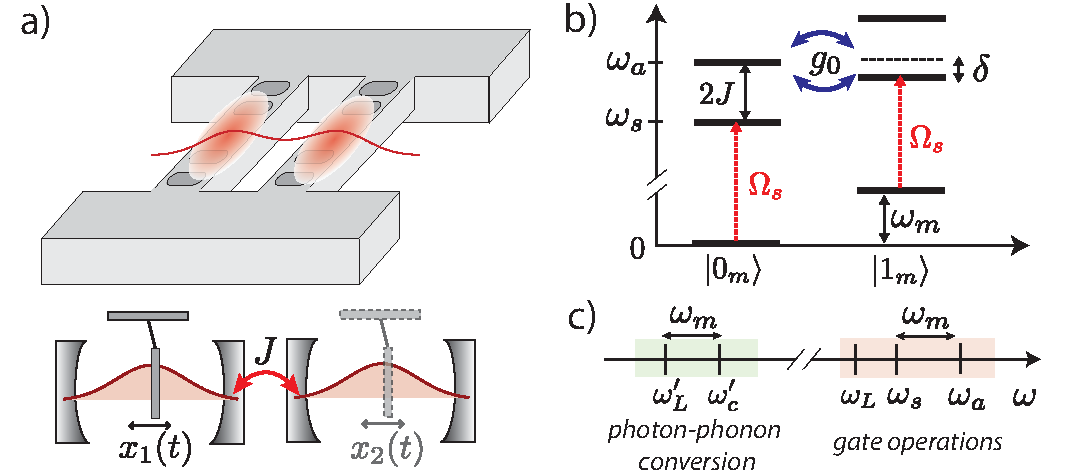
\includegraphics[width=0.9\textwidth]{./figs_Stannigel2012/Figure1.pdf}
\caption
[Model of two resonators]
{ a) Setup of two tunnel-coupled OM crystal cavities (see
Ref.~\cite{Eichenfield2009,Chan2011} for more details).  b) Level
diagram showing the lowest mechanical and optical excitations in a two mode OMS.
Resonant coupling $(\delta=0)$ occurs when the tunnel splitting $2J$ between the
optical modes is comparable to the mechanical frequency $\omega_m$. c) Different
sets of strongly and weakly coupled optical modes and control laser fields can
be used for nonlinear interactions $(\omega_{s},\omega_{a},\omega_L)$ and purely
linear photon storage and retrieval operations
$(\omega_c^\prime,\omega_L^\prime)$.
}
\label{fig:Setup}
\end{center} 
\end{figure}


\section{Model} 

We consider a setup of two tunnel-coupled
OMSs~\cite{Miao2009,Grudinin2010,Dobrindt2010,Safavi-Naeini2011a,Cheung2011}
as schematically shown in Fig.~\ref{fig:Setup}, focusing on the OM crystal
design~\cite{Eichenfield2009,Chan2011} as a specific example.
Each OMS $i=1,2$ is represented by an optical mode of frequency $\omega_c$ and a
bosonic operator $c_{i}$, which is coupled via optical gradient forces to the
motion of an isolated mechanical mode $b_i$ with vibrational frequency
$\omega^i_m$.  The Hamiltonian for this system is $(\hbar=1)$
\begin{equation}\label{eq:H}
\begin{split}
H= &\sum_{i=1,2} \omega_m^i b_i^\dag b_i +  \omega_c c_i^\dag c_i + g_0 c_i^\dag
c_i (b_i+ b_i^\dag) \\
&- J (c_1^\dag c_{2} + c_{1} c_{2}^\dag) +   \sum_{i=1,2}  \Omega_i ( c_i 
e^{i\omega_L t} + �{\rm H.c.}),
\end{split}\end{equation}
where $J$ is the tunneling amplitude between the optical modes and $g_0$ denotes
the single-photon OM coupling; $\Omega_i$ are the local amplitudes of external
control laser fields of frequency $\omega_L$.  Below we also consider an
additional set of cavity modes and driving fields with frequencies
$\omega_c^\prime $ and  $\omega_L^\prime$, respectively.
As indicated in Fig.~\ref{fig:Setup}(c), we assume these modes to be separated
in frequency and used for cooling the mechanical 
modes~\cite{WilsonRaePRL2007, MarquardtPRL2007}, and linear photon storage and
retrieval operations~\cite{Fiore2011, Verhagen2011, Zhang2003, Akram2010} only. 

Apart from the coherent dynamics described by Eq.~\eqref{eq:H}, we include
dissipation through cavity decay and mechanical damping and model the evolution
of the system density operator $\rho$ by a master equation (ME)
\begin{equation}\label{eq:ME}
\begin{split}
\dot \rho = &-i[H,\rho] + \sum_{i}  \kappa \mathcal{D}[c_i] \rho +
\mathcal{L}_\gamma \rho, \\
\end{split} 
\end{equation}
where  $\mathcal{D}[c]\rho=2c\rho c^\dag-\{c^\dag c, \rho\}_+ $, and
$\mathcal{L}_\gamma =\sum_i \frac{\gamma}{2}  (N_{\rm th}+1)   \mathcal{D}[b_i]
+ \frac{\gamma}{2}  N_{\rm th}  \mathcal{D}[b_i^\dag]$.
Here,  $\kappa$ is the optical field decay rate, $\gamma=\omega_m/Q$ the
mechanical damping rate for a quality factor $Q$ and $N_{\rm th}=(e^{\hbar
\omega_m/k_BT}-1)^{-1}$ the mechanical equilibrium occupation number for
temperature $T$. Below we identify $\Gamma_m=\frac{\gamma}{2}(3N_{\rm
th}+\frac{1}{2})$ as the characteristic decoherence rate for mechanical qubit
states\footnote{$\Gamma_m$ corresponds to the initial decoherence rate of a
phonon superposition $(|0_m\rangle+|1_m\rangle)/\sqrt{2}$.}.
\begin{figure}
\begin{center}
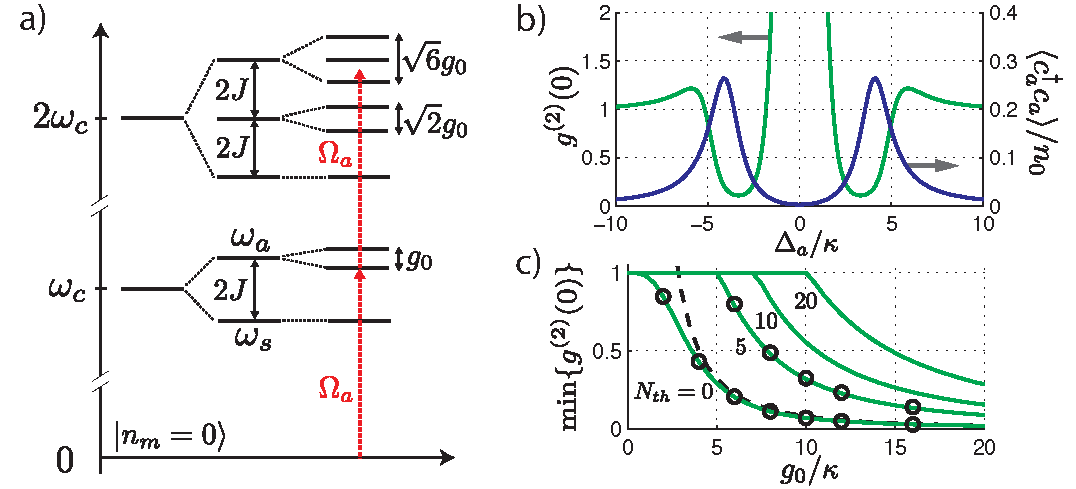
\includegraphics[width=1\textwidth]{./figs_Stannigel2012/Figure2.pdf}
\caption
[Behavior of the coupled system]
{a) Energy level diagram of a resonantly coupled OMS,
$\delta=2J-\omega_m=0$, and for a single mechanical mode in the ground state. b)
Excitation spectrum and $g^{(2)}(0)$ for a weak coherent field exciting the
$c_a$ mode, where $g_0/\kappa=8$ and $n_0=\Omega^2_a/\kappa^2$.  c) Minimal
value of $g^{(2)}(0)$  as a function of the OM coupling strength $g_0$ and for
different values of $N_{\rm th}$. The analytical results (solid lines) given in
the text are in good agreement with exact numerics (circles). The dashed line
shows the asymptotic scaling $\sim 8\kappa^2/g_0^2$ at zero temperature.}
\label{fig:ResonantLevels}
\end{center} 
\end{figure}



\section{Resonant strong-coupling optomechanics}
 
We focus on the strong coupling regime $\omega_m,g_0\gg \kappa,\Gamma_m$,  and
our main goal is to show how the multimode OMS described by Eq.~\eqref{eq:H} can
be used for implementing controlled interactions between qubits encoded in
photonic or phononic degrees of freedom.  To illustrate this we first consider a
single mechanical resonator, $b\equiv b_1$, $\omega_m\equiv \omega_m^1$. We
introduce symmetric and antisymmetric optical modes $c_{s,a}=  \left( c_1 \pm
c_2\right)/\sqrt{2}$ with eigenfrequencies $\omega_{s,a}$ split by $2J$.
Further, we assume that $\omega_m\sim 2J \gg g_0,\kappa, |\delta|$, where
$\delta=2J-\omega_m$  (see Fig.~\ref{fig:Setup}(b)). This condition can be
achieved in nanoscale OMSs where $\omega_m\sim $
GHz~\cite{Eichenfield2009,Chan2011,Carmon2007,Ding2011} and a
matching tunnel splitting can be designed by appropriately adjusting the spacing
between the cavities~\cite{Eichenfield2009,Grudinin2010}. In this
regime we can make a rotating wave approximation with respect to the large
frequency scale $\omega_m \sim 2J$ and after changing into a frame rotating with
$\omega_L$ we obtain~\cite{Grudinin2010}
\begin{equation}\label{eq:HRWA}
H= - \Delta_s c_s^\dag c_s - \Delta_a  c_a^\dag c_a   + \omega_m b^\dag b 
+ \frac{g_0}{2} (c_a c_s^\dag b^\dag +    c_a^\dag c_s  b)+ H_\Omega(t).
\end{equation}
Here $ \Delta_{s,a}= \omega_L - \omega_{s,a}$ are the detunings of the driving
field from the $c_s$ and $c_a$ mode, respectively, and
$H_\Omega(t)=\sum_{\eta=s,a} \left(\Omega_\eta(t) c_\eta + {\rm H.c.}\right)$
accounts for the external driving fields with slowly varying amplitudes
$\Omega_{s,a}(t)=(\Omega_1(t)\pm\Omega_2(t))/\sqrt{2}$.

The two-mode OM coupling in Eq.~\eqref{eq:HRWA} describes  photon transitions
between the energetically higher mode $c_a$ to the lower mode $c_s$, while
simultaneously absorbing or emitting a phonon.  For
$(\Delta_s-\Delta_a-\omega_m)=\delta=0$, this leads to a resonant interaction
between states $|n_a,n_s,n_m\rangle$ and $|n_a-1,n_s+1,n_m+1\rangle$, where
$n_a$, $n_s$ and $n_m$ label the occupation numbers of the two optical modes and
the mechanical mode, respectively.  In analogy to atomic cavity quantum
electrodynamics (QED)~\cite{CavityQEDReview}, the nonlinear scaling of the
corresponding transition amplitudes $\frac{g_0}{2} \sqrt{n_a (n_s+1) (n_m+1)}$
results in an anharmonic level diagram as shown in
Fig.~\ref{fig:ResonantLevels}(a).  If $g_0$ exceeds the cavity linewidth
$\kappa$, one and two photon transitions can be spectrally resolved, indicating
the onset of strong single-photon nonlinearities.


\section{An OM single-photon source}
 
As a potential first application of the nonlinear OM interaction we discuss the
use of the OMS as a single-photon source, which is characterized by a vanishing
equal time two-photon correlation function $g^{(2)}(0)$.  In
Fig.~\ref{fig:ResonantLevels}(b) we plot the excitation spectrum $\langle
c_a^\dag c_a \rangle$ and $g^{(2)}(0)=\langle c_a^\dag c_a^\dag c_a
c_a\rangle/\langle c_a^\dag c_a\rangle^2$,  for the case where only the $c_a$
mode is weakly driven. Around the single-photon resonances $\Delta_a=\pm g_0/2$
we observe strong anti-bunching $g^{(2)}(0)<1$ as a clear signature of
non-classical  photon statistics. To quantify this effect we assume that
$\Gamma_m \ll\kappa$, which allows us to treat subspaces connected to different
$|n_m\rangle$ separately.  For weak driving fields $\Omega_a\ll\kappa$, the
system dynamics can then be restricted to the  six states $ |0_a,0_s,
n_m\rangle, |1_a,0_s, n_m\rangle,|0_a,1_s, n_m+1\rangle,|2_a,0_s, n_m\rangle,
|1_a,1_s, n_m+1\rangle,|0_a,2_s, n_m+2\rangle$ and  we calculate the relevant
occupation probabilities $p_{1,0,n_m}$ and  $p_{2,0,n_m}$ to leading order in
$\Omega_a$~\cite{Carmichael1991}.
We obtain
\begin{equation}
p_{1,0,n}=\abs{ \frac{4\Omega_a d}{ X_n}}^2, \qquad p_{2,0,n} = 8 \abs{
\frac{\Omega_a^2 (8 d^2 - g_0^2)}{( X_n (2X_n -g_0^2))}}^2,
\end{equation}
where $d = \Delta_a - i\kappa$ and $X_n=d^2-g_0^2(n+1)$. By taking the
appropriate thermal averages, $\ev{n_a} = \sum_n \zeta_n p_{1,0,n}$ and
$g^{(2)}(0)  = 2 \sum_n \zeta_n p_{2,0,n}/\ev{n_a}^2$, where
$\zeta_n=(1-e^{-\beta \hbar \omega_m})e^{-\beta \hbar \omega_m n}$ and
$\beta^{-1}=k_B T$, the two photon correlation function can be evaluated for
arbitrary temperatures $T$.

In Fig.~\ref{fig:ResonantLevels}(c) we plot the minimal value of $g^{(2)}(0)$ as
a function of the coupling strength $g_0$ and for different $N_{\rm th}$.
As the OM coupling increases we find that for $T=0$ the minimum of the
correlation function scales as $\textrm{min}_{\Delta_a}\{g^{(2)}(0)\}\simeq 8
\kappa^2/g_0^2$. This demonstrates an improved scaling over off-resonant photon
blockade effects in single-mode OMSs, where for large $\omega_m$ only a small
reduction $g^{(2)}(0)\simeq 1-g_0^2 /(\kappa \omega_m)$ can be
obtained~\cite{Rabl2011}. Since the positions of the single and two-photon
resonances depend explicitly on the mechanical state $|n_m\rangle$,  finite
temperature degrades the quality of the single-photon source.  Nevertheless,
with increasing coupling strength the anti-bunching effect becomes surprisingly
robust and when combined with cooling cycles to achieve $\langle n_m\rangle \sim
1$~\cite{Chan2011}, allows the operation of OM single-photon sources even
at environmental temperatures of a few Kelvin.
\begin{figure}
\begin{center}
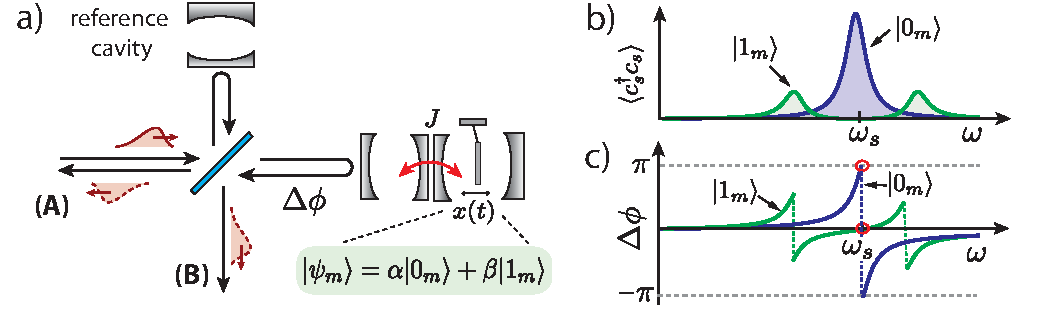
\includegraphics[width=1\textwidth]{./figs_Stannigel2012/Figure3.pdf}
\caption
[A single-phonon single-photon transistor]
{a) An incoming
photon in port (A) passes through the interferometric setup and leaves through
port (A) or (B), depending on the phase shift $\Delta \phi$ acquired upon
reflection from the two-mode OMS.   b), c) For a mechanical system in state
$|0_m\rangle$, the OMS exhibits a single resonance at $\omega_s$ $(\Delta
\phi=\pi$), while for state $|1_m\rangle$  the resonance splits by $g_0\gg
\kappa $ and the photon does not enter the cavity $(\Delta \phi=0)$.  }
\label{fig:SinglePhononTransistor}
\end{center} 
\end{figure}

\section{Single-phonon single-photon transistor}  
Given the ability to generate single photons,
Fig.~\ref{fig:SinglePhononTransistor} illustrates a basic scheme for using the
same resonant OMS to implement a two-qubit gate~\cite{DuanPRL2004}. First, we
assume that the state of a control photon is mapped onto a mechanical
superposition state  $\alpha|0_m\rangle+\beta |1_m\rangle$.
This can be achieved with conventional cooling followed by photon-phonon
conversion techniques using linearized OM interactions with an auxiliary mode
$\omega_c^\prime$ (see Fig.~\ref{fig:Setup}(c)). Next, a single target photon of
central frequency $\sim \omega_s$ is sent through the interferometric setup as
described in Fig.~\ref{fig:SinglePhononTransistor}.
If the mechanical mode is in the state $|0_m\rangle$,  the incoming photon
couples to a single resonant state $|0_a,1_s,0_m\rangle$ (see
Fig.~\ref{fig:Setup}(b)), such that it enters the cavity and picks up a phase
before being reflected.  Instead, if the mechanical resonator is in the state 
$|1_m\rangle$,  the resonant coupling between $|0_a,1_s,1_m\rangle$ and
$|1_a,0_s,0_m\rangle$ splits the cavity resonance, and for $g_0>\kappa$ the
photon is reflected without a phase shift.
Under ideal conditions,  the final result is an entangled state
\begin{equation}\label{eq:Entangled}
|\psi\rangle = \alpha | 0_m, 1_A,0_B\rangle + \beta | 1_m, 0_A,1_B\rangle,
\end{equation}
where $A$ and $B$ are the two ports of the interferometer. This state can be
converted back into an entangled state between the initial control and target
photon.

Assuming that the storage and retrieval of the control photon can be achieved
with high fidelity, the error for producing the entangled
state~\eqref{eq:Entangled} with $\alpha=\beta=1/\sqrt{2}$ is approximately given
by
\begin{equation}\label{eq:Error}
\epsilon  \approx  \frac{4\kappa^2}{g_0^2}+  \frac{1}{(\tau_p \kappa)^{2}}+ 
\tau_p \Gamma_m,
\end{equation} 
where  $\tau_p$ is the duration of the single-photon pulse. The individual
contributions in Eq.~\eqref{eq:Error} arise from an imperfect photon reflection,
the finite spectral width of the photon pulse, and mechanical decoherence,
respectively.
A minimal error is achieved for  $\tau_p^{-1}\approx \sqrt[3]{\kappa^2
\Gamma_m}$ where we obtain $\epsilon\approx {\rm  max} \{  4\kappa^2/g_0^2,
\sqrt[3]{\Gamma_m^2 /\kappa^2}\}$.
Assuming an OM crystal device with $\omega_m/(2\pi)=4$ GHz and $Q=10^5$ as
discussed in Ref.~\cite{Chan2011}, but with an improved OM coupling
$g_0/(2\pi)=50$ MHz and a lower  decay rate $\kappa/(2\pi)=5$ MHz, we obtain
gate errors $\epsilon\approx 0.1$ for environmental temperatures around
$T\approx 100$ mK.




\section{Phonon-phonon interactions}
  
Finally, we consider the possibility to perform a 
controlled gate operation between two qubits stored
in long-lived mechanical modes.
Our approach is depicted 
in Fig.~\ref{fig:PhononQuantumGate}(a), 
and combines the long coherence times of an OM 
quantum memory~\cite{Fiore2011,Verhagen2011,Zhang2003,Akram2010} 
with the practical utility of exploiting interactions 
between stationary phononic qubits.
We focus on the limit $\Gamma_m\ll \kappa$, 
and assume that optical (e.g. `path encoded') 
qubits are first mapped onto long-lived states $|0_m\rangle$ 
and $|1_m\rangle$ of two or more mechanical modes.
The OM coupling is then employed to generate 
nonlinear interactions between the phonons only.  
\begin{figure}
\begin{center}
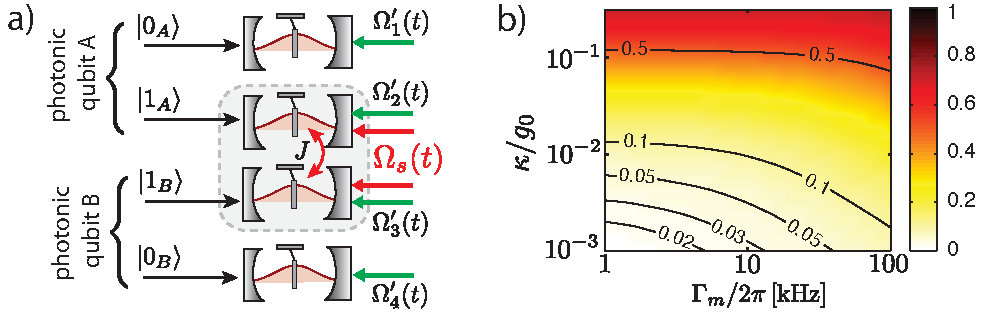
\includegraphics[width=1\textwidth]{./figs_Stannigel2012/Figure4.pdf}
\caption
[Controlled phase gate]
{a) OM quantum memory, where `path-encoded' photonic
qubits are stored in long-lived mechanical states using tunable linearized OM
interactions $\sim\Omega^\prime_i(t)$. Deterministic gate operation between
stationary qubits are implemented by a controlled phonon-phonon interaction
$\sim\Omega_s(t)$ as described in the text. b) The total error $\epsilon_g$ for
implementing a controlled phase gate between two phononic qubits is minimized
with respect to $\Delta_s$ and plotted as a function of $\kappa$ and $\Gamma_m$
(see text). The parameters for this plot are $g_0/(2\pi)=50$ MHz,
$\gamma/(2\pi)=4$ kHz, $\alpha=1$ and $g_0/\delta=1/3$.
}
\label{fig:PhononQuantumGate}
\end{center} 
\end{figure}


We consider nonlinear interactions between
two mechanical modes $b_1$ and $b_2$ described
by Eq.~\eqref{eq:H}, detuned from resonance such that
$g_0< |(2J-\omega_m^i)|$ and direct transitions between  
photons and phonons are suppressed. 
To obtain the effective phonon-phonon interactions,
we first diagonalize
$H$ to second order in $\xi_i = g_0/(2J-\omega_m^i)$
with the transformation
$H\rightarrow e^{iS}He^{-iS}$, 
where 
$S=\frac{i}{2} (c_s^\dag c_a (\xi_1b_1^\dag-\xi_2b_2^\dag) -{\rm H.c.})$.
This yields
 $H= H_0 +H_g+H_\Omega(t)$, where $H_0=  - \Delta_s c_s^\dag c_s - \Delta_a 
 c_a^\dag c_a   + \sum_i \omega^i_m b_i^\dag b_i$,
\begin{equation}\label{eq:Hoff}
	H_g= \frac{g_0}{4} \left[ (c_s^\dag c_s\!+\!1)c^\dag_a c_a (\xi_1\!+\!\xi_2) 
	+ (c_a^\dag c_a\! -\!	c_s^\dag c_s) \mathcal{N}_b \right],
\end{equation}
and we have neglected small corrections to the driving Hamiltonian
$H_\Omega(t)$.
The phonon operator in Eq.~\eqref{eq:Hoff} is given by $\mathcal{N}_b= \xi_1
b_1^\dag b_1+\xi_2 b_2^\dag b_2 - (\xi_1+\xi_2)(b_1^\dag b_2+ b_2^\dag b_1)/2$.
For simplicity we focus on symmetric detuning, $\omega_m^{1,2} = 2J\mp \delta$,
where $\mathcal{N}_b=\frac{g_0}{\delta}(b_1^\dag b_1-b_2^\dag b_2)$.
The  transformation also modifies the dissipative terms in the
Eq.~\eqref{eq:ME}; most importantly, we find an optically-induced decay channel
for the mechanical modes, $\mathcal{L}_\gamma\rightarrow \mathcal{L}_\gamma +
\kappa g^2_0/(4\delta^2) \mathcal{D}[c_s (b_1+b_2)]$.

We assume that only the $c_s$ mode is weakly 
driven by a slowly-varying control field $\Omega_s(t)$. 
In this case the $c_a$ mode remains unpopulated and 
we neglect it. 
Next, we shift the driven mode, $c_s\rightarrow \alpha + c_s$, 
by the classical amplitude $\alpha$,
yielding an effective ME  for $c_s$, $b_1$ and $b_2$.
Finally, we adiabatically eliminate the $c_s$ mode, valid in the
limit $|\alpha|\sim \mathcal{O}(1)$ and $(g_0^2|\alpha|/4\delta)\ll
|\Delta_s+i\kappa|$,
to obtain an effective ME for the mechanical modes (see Appendix
\ref{app:Stannigel2012} for more details), 
\begin{equation}\label{eq:Effective}
\begin{split}
\dot \rho_m =& -i[H_m + \Lambda (b_1^\dag b_1-b_2^\dag b_2)^2 �, \rho_m ] 
+\mathcal{L}_\gamma \rho_m\\
&+ \Gamma_\phi \mathcal{D}[(b_1^\dag b_1-b_2^\dag b_2)]\rho_m   + 
\frac{\gamma^\prime}{2} \sum_i   \mathcal{D}[b_i]\rho_m.
\end{split} 
\end{equation}
Here, $\gamma^\prime=\kappa |\alpha|^2 g_0^2/(2\delta^2)$, and the phonon-phonon
interaction and the phonon dephasing rate are given by
\begin{equation}
\Lambda=\frac{g_{0}^{4}|\alpha|^2  \Delta_{s}}{16 \delta^2
(\Delta_{s}^{2}+\kappa^{2})},\qquad \Gamma_\phi= \frac{g_{0}^{4}|\alpha|^2 
\kappa}{16\delta^2(\Delta_{s}^{2}+\kappa^{2})}.
\end{equation}
The effective Hamiltonian in Eq.~\eqref{eq:Effective} describes 
a phonon nonlinearity with a tunable strength $\Lambda(t)\sim |\alpha(t)|^2$. 
The relevant cross-coupling is given by 
\begin{equation}\label{eq:Heff}
H_{\rm int} \simeq 2 \Lambda b_1^\dag b_1  b_2^\dag b_2,
\end{equation}
and when acting for a time $t_g=\pi/(2\Lambda)$, this Hamiltonian implements a
controlled-phase gate between two qubits encoded in states $|0_m\rangle$ and
$|1_m\rangle$.
During this time, phonons experience intrinsic and optically-induced decoherence
as seen in Eq.~\eqref{eq:Effective}.
In Fig.~\ref{fig:PhononQuantumGate}, we plot the
resulting gate error $\epsilon_g=1-\langle\psi_0|\rho_m(t_g)|\psi_0\rangle$  
for an initial state
$|\psi_0\rangle=\frac{1}{2}(|0_m\rangle+|1_m\rangle)^{\otimes2}$
optimized with respect to $\Delta_s$.
Using the total decoherence rate of this state, 
$\Gamma_{\rm decoh}= 2\Gamma_m+ \Gamma_\phi+ \gamma^\prime/2$, 
we find that  $\epsilon_g\propto\Gamma_{\rm decoh}/\Lambda$ 
is minimized for $|\Delta_s|\simeq g_0/2$, where $\epsilon_g\propto
4(\kappa/g_0)$.
While this scaling with $g_0$ is weaker than for a gate based on photon
reflection (see Eq.~\eqref{eq:Error}), the ability to perform a gate between
stationary qubits represents an important advantage of this approach.

 
\section{Conclusions} 

We have described single-photon and single-phonon nonlinear effects in strongly
coupled multimode OMSs. We have shown how induced nonlinearities on or near
resonance can be used for controlled quantum gate operations between flying
optical or stationary phononic qubits. Our results provide a realistic route
towards the quantum nonlinear regime of OMSs, and a framework for future OM
information processing applications.
 
\chapter{Heralded Quantum Gates with Integrated Error Detection}
\label{ch:Borregaard_PRL2015}
%%%%%%%%%%%%%%%%%%%%%%%%%%%%%%%%%%%%%%%%%%%%%%%%

\section{Introduction}
%From \cite{Borregaard2015a}

Exploiting quantum systems for information processing offers many potential
advantages over classical information processing like highly secure quantum
networks~\cite{cirac,kimble, duan3} and powerful quantum
computers~\cite{ladd,shor,feynman}. One of the main challenges for the
realization of functional quantum computers is to perform gates with
sufficiently high quality so that the remaining errors can be suppressed by
error correction codes, which makes the computation fault tolerant
\cite{knill2}. At the same time, applications to long distance quantum
communication can be enabled by quantum repeaters, which combine probabilistic
entanglement generation over short distances with subsequent entanglement
connection steps \cite{duan3}. For these protocols, the probabilistic nature of
the entanglement generation is acceptable, but it is essential that high
fidelity entanglement is achieved conditioned on a heralding measurement.
Experimentally, such high fidelity entanglement is often much easier to
implement and may be realized in situations where it is impossible to perform
any quantum operations deterministically. Here we introduce a similar concept
for gate operations and develop the concept of  heralded quantum gates  with
integrated error detection. In the resulting gate, the infidelity, which would
be present for a deterministic gate is converted into a failure probability,
which is heralded by an auxiliary atom. Once successful, the resulting gate can
have an arbitrarily small error. Such heralded gates could facilitate fault
tolerant quantum computation since detectable errors may be easier to correct
than undetectable errors~\cite{grassi,ralph05,varnava}.  Alternatively it can be
directly incorporated into quantum repeater architectures for long distance
quantum communication.

Optical cavities are ideal for conversion between the stationary gate qubits and
flying qubits (photons), which is fundamental for quantum networks \cite{ritter,
Komar2014, acin}. Quantum gates can, in principle, also be directly implemented in
optical cavities \cite{pellizari}, but the experimental requirements for this
are very challenging due to spontaneous emission and cavity loss. The essential
parameter quantifying this is the cooperativity of the atom-cavity system, $C$.
It has been argued that directly implementing gates in optical cavities leads to
a poor error scaling $1-F\propto1/\sqrt{C}$, where $F$ is the fidelity of the
gate \cite{kastoryano, Anders2prl}. However, as a result of the integrated error
detection, the heralded gates that we propose exhibit high fidelities when
successful. This enables efficient entanglement swapping and removes the
necessity of intermediate entanglement purification in quantum repeaters thus
increasing the distribution rate significantly. Compared to using other
deterministic, cavity based gates, an increase in the rate of up to two orders
of magnitude can be achieved for modest cooperativities ($<100$) and a distance
of 1000 km \cite{Borregaard2015b}.

\section{Heralding gate}

The basic idea is to use a heralding auxiliary atom in addition to qubit atoms
in the same cavity. One of the atomic qubit states, e.g., state $\ket{1}$
couples to the cavity mode while $\ket{0}$ is completely uncoupled (see
\reffig{fig:levels}(a)). Such a system has previously been considered for two-qubit
gates~\cite{duan1, DuanPRL2004, Anders1prl, Anders2prl,ritter2014}, multi-qubit
gates~\cite{duan1,zheng} and photon routing~\cite{Tiecke}.
If any of the qubit atoms is in state $\ket{1}$ the cavity resonance is shifted
compared to the bare cavity mode, which can be exploited to make a gate between
two or more qubits by reflecting single photons off the cavity \cite{duan1}. The
efficiency of such schemes, however, is limited by photon losses, inefficient
detectors and non-ideal single photon sources \cite{Tiecke,ritter2014}. We
circumvent these problems by introducing an auxiliary atom in the cavity to
serve as both an intra-cavity photon source and a detector. As opposed to
previous heralded gates in optical cavities, which relied on the null detection
of photons leaving the cavity \cite{pachos,beige, vitali}, the final heralding
measurement on the atom can then be performed very efficiently.

In our approach, the auxiliary atom has two metastable states $\ket{g},\ket{f}$,
which can be coupled through an excited state $\ket{E}$ (see
\reffig{fig:levels}(a)). We assume the $\ket{E}\leftrightarrow\ket{f}$ transition
to be energetically close to the cavity frequency and to be a nearly closed
transition,  so that we need to drive the $\ket{g}\to \ket{E}$ transition, e.g
with a two-photon process, (see below).
The gate can be understood through the phase evolution imposed on the atoms. We
consider adiabatic excitation of the auxiliary control atom via Stimulated Raman
Adiabatic Passage~\cite{stirap,stirap2}, driven by an external driving pulse
with Rabi frequency $\Omega(t)$ and a coupling to the cavity photon $g_{f}$. In
the case when all the qubit atoms are in the non-coupled states $|00..0\rangle$,
an adiabatic excitation will result in a dark state $\sim g_{f} \ket{0,g}
-\Omega \ket{1,f}$ with zero energy and vanishing phase. Here the number refers
to the number of cavity photons.  However, the qubit states $\Psi$ with at least
one of the qubit atoms in the coupled state, results in a cavity-induced shift
of the state $|1,f, \Psi\rangle$, which in turn, causes an AC Stark shift and
dynamical phase to be imprinted into the $|g,\Psi\rangle$ state after the
driving pulse is turned off. All states but the completely uncoupled qubit state
$|00...0\rangle$ will thus acquire a phase, the magnitude of which depends on
the length of the driving pulse. With an appropriate pulse length and simple
single qubit rotations, we can use this to realize a general $N$-qubit Toffoli
gate or a control-phase (CZ) gate.

Naively, the gates will be limited by errors originating from cavity decay and
spontaneous emission from the atoms, which carry away information about the
qubit state. These errors are, however, detectable since the auxiliary atom will
be trapped in state $\ket{f}$ if either a cavity excitation or an atomic
excitation is lost. Conditioning on detecting the auxiliary atom in state
$\ket{g}$ at the end of the gate thus rules out the possibility of any
dissipative quantum jumps having occurred during the gate. As a result, the
conditional fidelity of the gate is greatly enhanced at the modest cost of a
finite but potentially low failure probability.
\begin{figure}
\centering
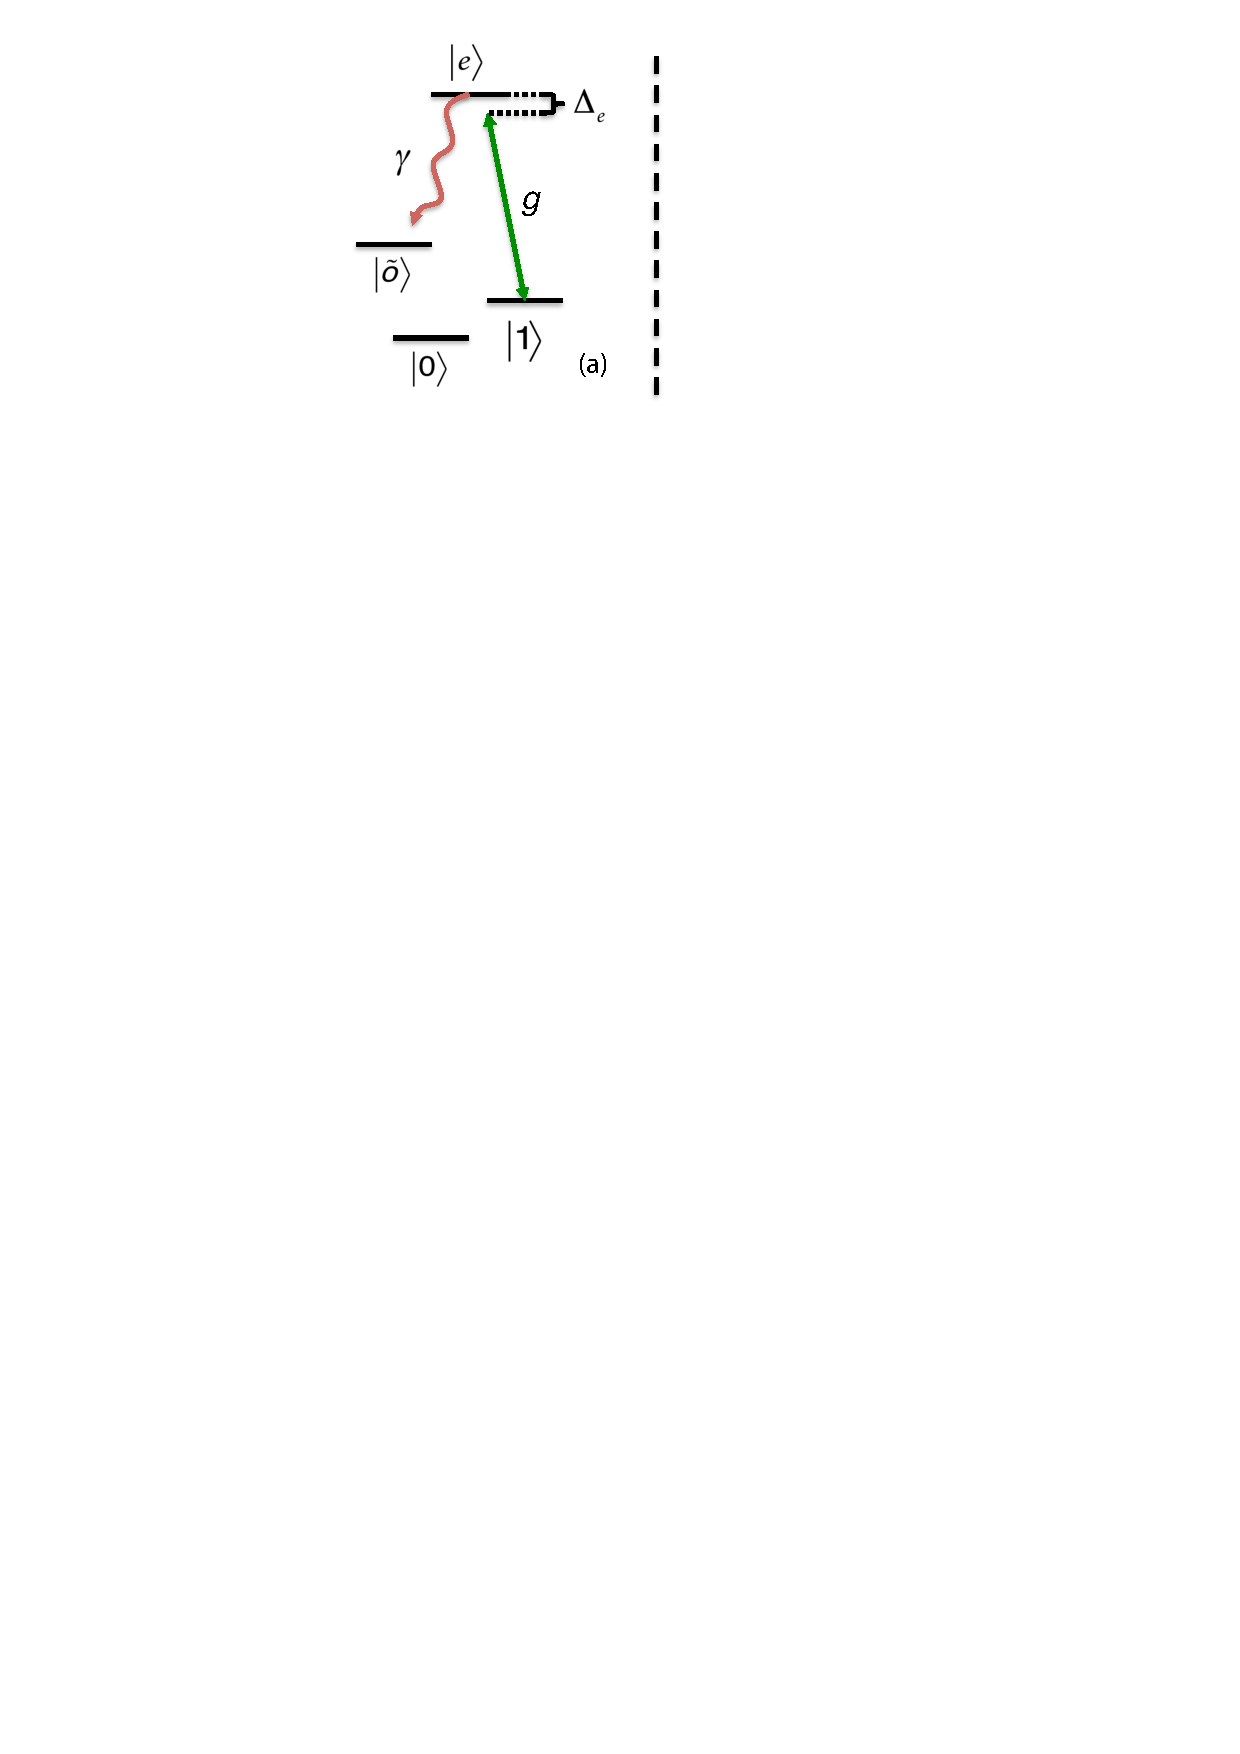
\includegraphics[width=0.35\textwidth]{./figs_Borregaard_PRL2015/figure1a} 
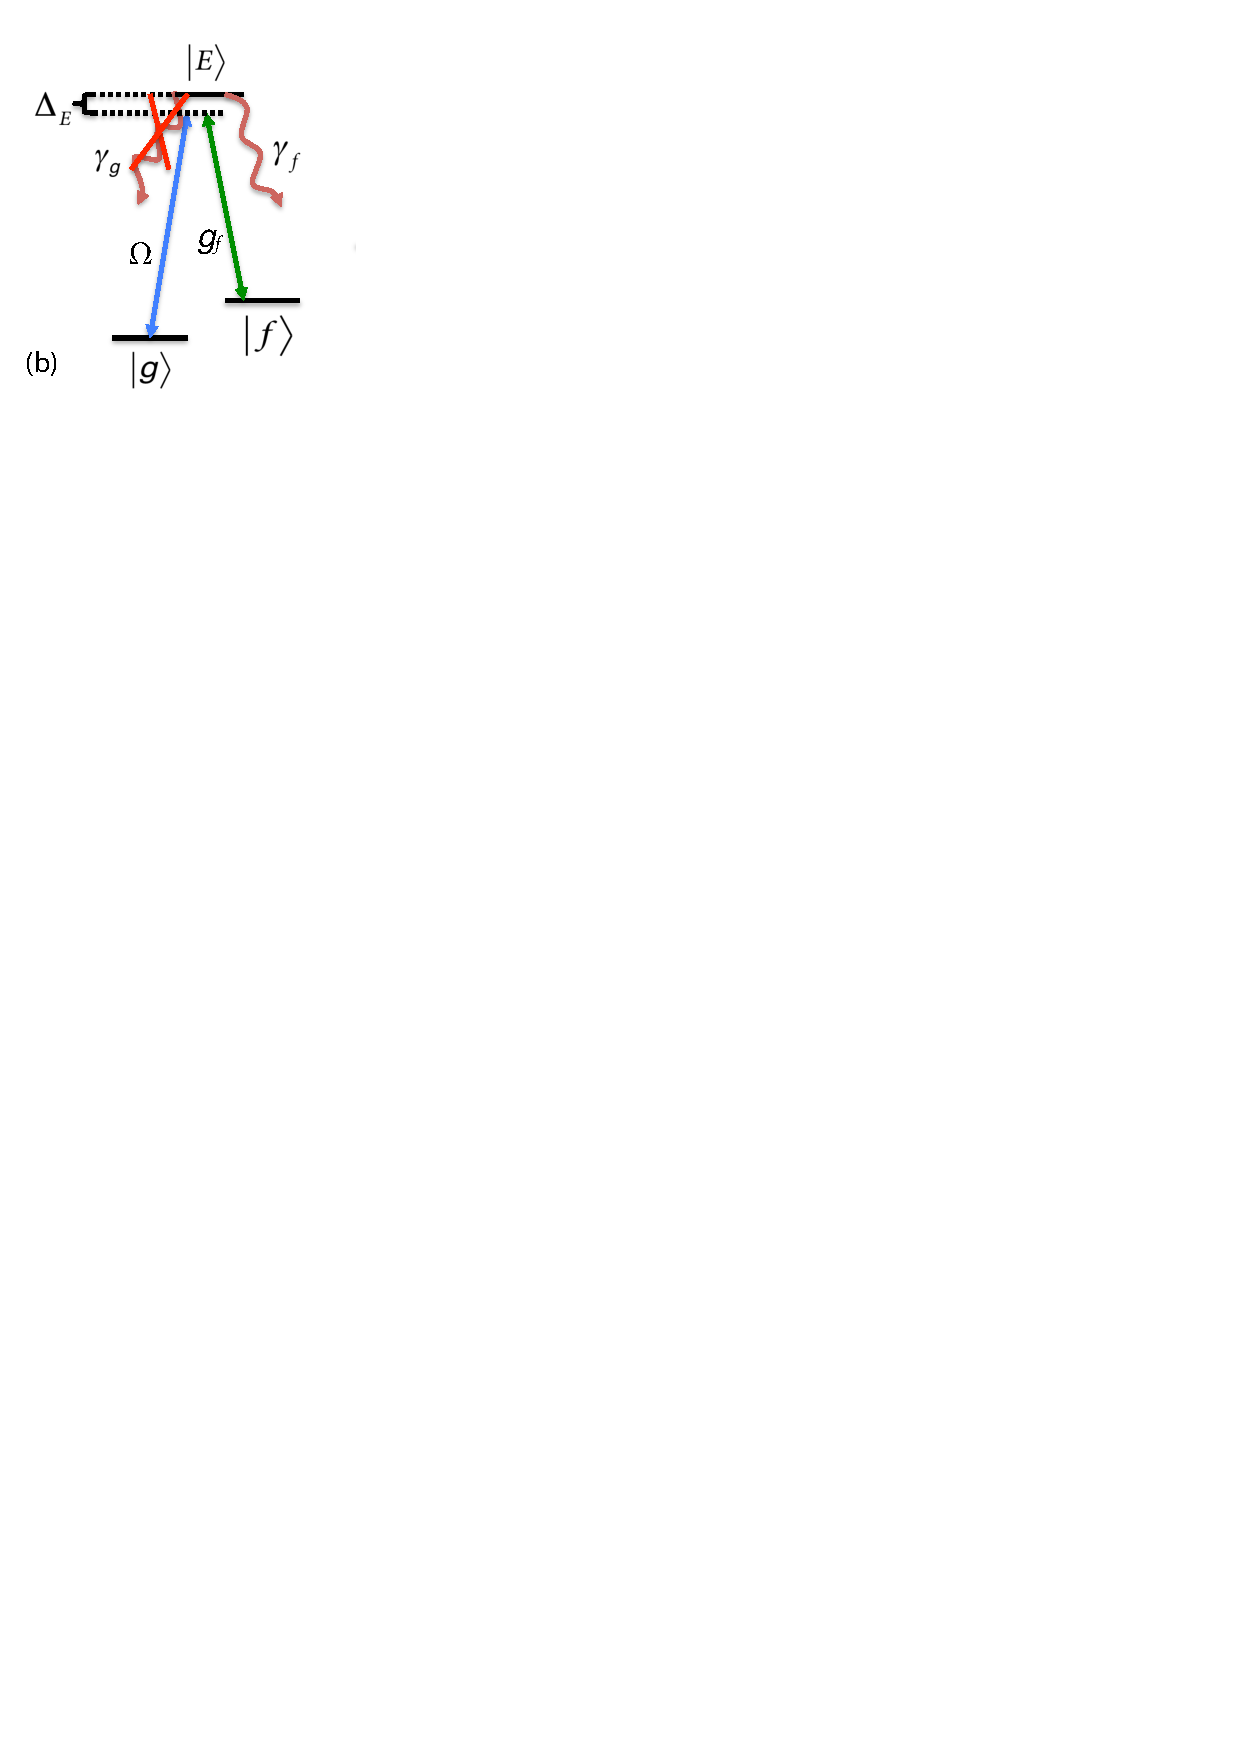
\includegraphics[width=0.35\textwidth]{./figs_Borregaard_PRL2015/figure1b}
\caption
[Level structures of qubit and control atoms]
{(a) Level structure of the qubit atoms. Only state $\ket{1}$ couples to
the cavity and we assume that the excited level decays to some level
$\ket{\tilde{o}}$, possible identical to $\ket{f}$ or $\ket{0}$. (b) Level
structure of the auxiliary atom and the transitions driven by the weak laser
($\Omega$) and the cavity ($g_{f}$). We assume that
$\ket{E}\leftrightarrow\ket{f}$ is a closed transition, i.e. $\gamma_{g}=0$.  }
\label{fig:levels}
\end{figure}

\section{Performance}

\subsection{Model}
We now analyze the performance of the gates and derive the success
probabilities, gate times and gate errors (see Tab.~S1 in Appendix
\ref{app:Borregaard_PRL2015}) The Hamiltonian in a proper rotating frame is (see
\reffig{fig:levels})
\begin{eqnarray} 
\hat{H}&=&
\Delta_{E}\ket{E}
\bra{E}+g_{f}(\hat{a}\ket{E}\bra{f}+H.c)+\hat{V}+\hat{V}^{\dagger} \nonumber \\
&&+\sum_{k}\Delta_{e}\ket{e}_{k}\bra{e}+g(\hat{a}\ket{e}_{k}\bra{1}+H.c),
\end{eqnarray}          
where $k$ labels the qubit atoms ($\hbar=1$), $2\hat{V}=\Omega\ket{E}\bra{g}$
and we have assumed that all couplings ($g,\Omega$) are real. We have defined
$\Delta_{E}=\omega_{E}-\omega_{g}-\omega_{L}$, and
$\Delta_{e}=\omega_{e}-\omega_{g}-\omega_{L}+\omega_{f}-\omega_{1}$, where
$\omega_{L}$ is the laser frequency and otherwise $\omega_{x}$ is the frequency
associated with level $x$. We describe the cavity decay and atomic spontaneous
emission with Lindblad operators so that $\hat{L}_{0}=\sqrt{\kappa}\hat{a}$
corresponds to the cavity decay,  $\hat{L}_{f}=\sqrt{\gamma_{f}}\ket{f}\bra{E}$
to the decay of the excited state of the auxiliary atom and
$\hat{L}_{k}=\sqrt{\gamma}\ket{\tilde{o}}_{k}\bra{e}$ describes the decay of the
excited qubit states to some arbitrary ground state $\ket{\tilde{o}}$. The
nature of $\ket{\tilde{o}}$ is not important for the dynamics of the gates and
it may or may not coincide with $\ket{0}$ or $\ket{1}$.

\subsection{Effective Hamiltonian}

We assume a weak driving pulse justifying for a perturbative treatment of
$\hat{V}$ using the formalism of Ref.~\cite{Florentin}. In the perturbative
description we adiabatically eliminate the coupled excited states of the atoms
and the cavity (assuming $\Omega^{2}/\Delta_{E}\!\ll\!\Delta_{E}$ and
$\Omega\!\ll\!g$), which leads to an energy shift of the ground states but
otherwise conserves them since the Hamiltonian cannot connect different
unexcited states without decay. The dynamics are therefore described by an
effective Hamiltonian,
$\hat{H}_{\text{eff}}=\ket{g}\bra{g}\sum_{n}\Delta_{n}\hat{P}_{n}$ where
\begin{equation}
\Delta_{n}=
\mathrm{Re}\left\{\frac{-\frac{\Omega^{2}}{4\gamma}
((\frac{\Delta_{e}}{\gamma}\!\!-\!\!i/2)i\!\!+\!\!2nC)}
{(2\frac{\Delta_{e}}{\gamma}\!\!-\!\!i)((2\frac{\Delta_{E}}{\gamma}
\!\!-\!\!i)i/4\!\!+\!\!C)\!\!+\!\!(2\frac{\Delta_{E}}{\gamma}\!\!-\!\!i)
nC}\right\}\label{eq:detunings}
\end{equation} 
and $\hat{P}_{n}$ projects on the states with $n$ qubits in state $\ket{1}$. For
simplicity, we have assumed that the auxiliary atom is identical to the qubit
atoms such that $g_{f}=g$ and $\gamma_{f}=\gamma$ (see Appendix
\ref{app:Borregaard_PRL2015} for a more general treatment) and we have defined
the cooperativity $C=g^{2}/\gamma\kappa$.
We consider the limit $C\gg1$ and from Eq.~\eqref{eq:detunings} we find that the
energy shift, in the case when all qubit atoms are in $\ket{0}$, becomes very
small $\Delta_{0}\sim\Delta_{E}\Omega^{2}/(16\gamma^{2} C^{2})\rightarrow 0$,
i.e., we drive into a zero energy dark state as mentioned in the description
above.
On the contrary, for $n>0$, the $C$ in the nominator of $\Delta_{n}$ reflects
that the coupling of the qubit atoms shifts the cavity resonance and as a result
an AC stark shift of $\sim\Omega^{2}/\Delta_{E}$ is introduced.
Furthermore, we find that in the effective evolution, errors caused by
spontaneous emission or cavity decay ($\hat{L}_{0},\hat{L}_{f},\hat{L}_{k}$)
project the system out of the effective space into orthogonal subspaces, which
allows for an efficient error detection by measuring the ancilla atom.

\subsection{Success probability}

The dynamics described by $\hat{H}_{\text{eff}}$ can be used to implement a
Toffoli gate. Assuming the qubit atoms to be on resonance $(\Delta_{e}=0)$ and
having $\Delta_{E}\sim\gamma\sqrt{C}$ gives energy shifts
$\Delta_{n>0}\sim\Omega^{2}/(4\gamma\sqrt{C})$ while
$\Delta_{0}\sim\mathcal{O}(\Omega^{2}/C^{3/2})$. Hence, $\ket{00...0}$ is the
only state, which remains unshifted and we can choose a gate time of
$t_{\text{T}}\sim4\pi\sqrt{C}\gamma/\Omega^{2}$ to make a Toffoli gate. By
conditioning on measuring the auxiliary atom in state $\ket{g}$ at the end of
the gate, the detectable errors from cavity decay and spontaneous emission only
reduce the success probability instead of reducing the fidelity. Consequently,
the fidelity becomes limited by more subtle, undetectable errors (see
Appendix \ref{app:Borregaard_PRL2015}). The dominant error originates from the
qubit dependent decay rate, $\Gamma_{n}$, of $\ket{g}\to\ket{f}$. As we
demonstrate in Appendix \ref{app:Borregaard_PRL2015}), this leads to a fidelity lower bounded by $1-F
\lesssim 0.3/C$, with a success probability of $P_{\text{s}} \sim 1 -
3/\sqrt{C}$. Thus is a substantial improvement over the leading error in the
case of deterministic cavity-assisted gates. For generic states, the fidelity
can even be markedly higher, and improving with increasing particle number $N$,
see Appendix \ref{app:Borregaard_PRL2015}.

In the special case of only two qubits, the Toffoli gate is referred to as a
CZ-gate, and in this case, we can even improve the gate to have an arbitrarily
small error by combining it with single qubit rotations. For the general Toffoli
gate discussed above, we needed $\Delta_e=0$ to ensure the correct phase
evolution, but making the single qubit transformations $\ket{0}\to
e^{-i\Delta_{0}t/2}\ket{0}$ and $\ket{1}\to
e^{-i(\Delta_{1}-\Delta_{0})t/2}\ket{0}$, at the end of a driving pulse of
length $t_{\text{CZ}}=\abs{\pi/(\Delta_{2}-2\Delta_{1}+\Delta_{0})}$, ensures
the right phase evolution of the CZ-gate without any constraints on
$\Delta_{e}$. Hence, it is possible to tune $\Delta_{e}$ to eliminate the
detrimental effect of having a qubit dependent decay rate. Choosing
$\Delta_{E}=\frac{\gamma}{2}\sqrt{4C+1}$ and
$\Delta_{e}=\frac{1}{2}C\gamma^{2}/\Delta_{E}$ ensures
$\Gamma_0=\Gamma_1=\Gamma_2$, and thus removes all dissipative errors from the
heralded gate. The conditional error is then limited only by non-adiabatic
effects, that can in principle be made arbitrarily small by reducing the driving
strength. The success probability is $1-P_{\text{s}}\sim 6/\sqrt{C}$ in the
limit $C\gg1$ (see \reffig{fig:prob}).
We thus have a heralded two qubit gate with arbitrarily small error with a
success probability that can approach 1 (it is possible to decrease the scaling
factor of the probability from $\sim6$ to $\sim3.4$ at the expense of an error
scaling as $1/C$ by tuning $\Delta_{E},\Delta_{e}$).

\subsection{Gate time}

We now consider the gate time. The gate time of the Toffoli gate is
$t_{\text{T}}\sim4\pi\sqrt{C}\gamma/\Omega^{2}$ and for the CZ-gate we have
$t_{\text{CZ}}\sim15\pi\sqrt{C}\gamma/(2\Omega^{2})$ for $C\gg1$. Since
$t_{\text{CZ}}>t_{\text{T}}$ we focus on $t_{\text{CZ}}$. The gate time is set
by the strength ($\Omega$) of the driving pulse, which is limited by
non-adiabatic errors. This is investigated in the supplemental material where we
also verify our analytical results numerically in Appendix
\ref{app:Borregaard_PRL2015}.
Assuming realisitc parameters of $\kappa=100\gamma$ \cite{thompson,Tiecke}, we find that a driving
of $\Omega=\sqrt{C}\gamma/4$ keeps the non-adiabatic error of the gate below
$4\cdot10^{-5}$ for $C\leq1000$. The gate times decreases as $1/\sqrt{C}$ as
shown in \reffig{fig:prob}. For a cooperativity of $100$ the gate time is
$\approx1$ $\mu$s  for typical atomic decay rates.
\begin{figure} 
\centering
$\vcenter{\hbox{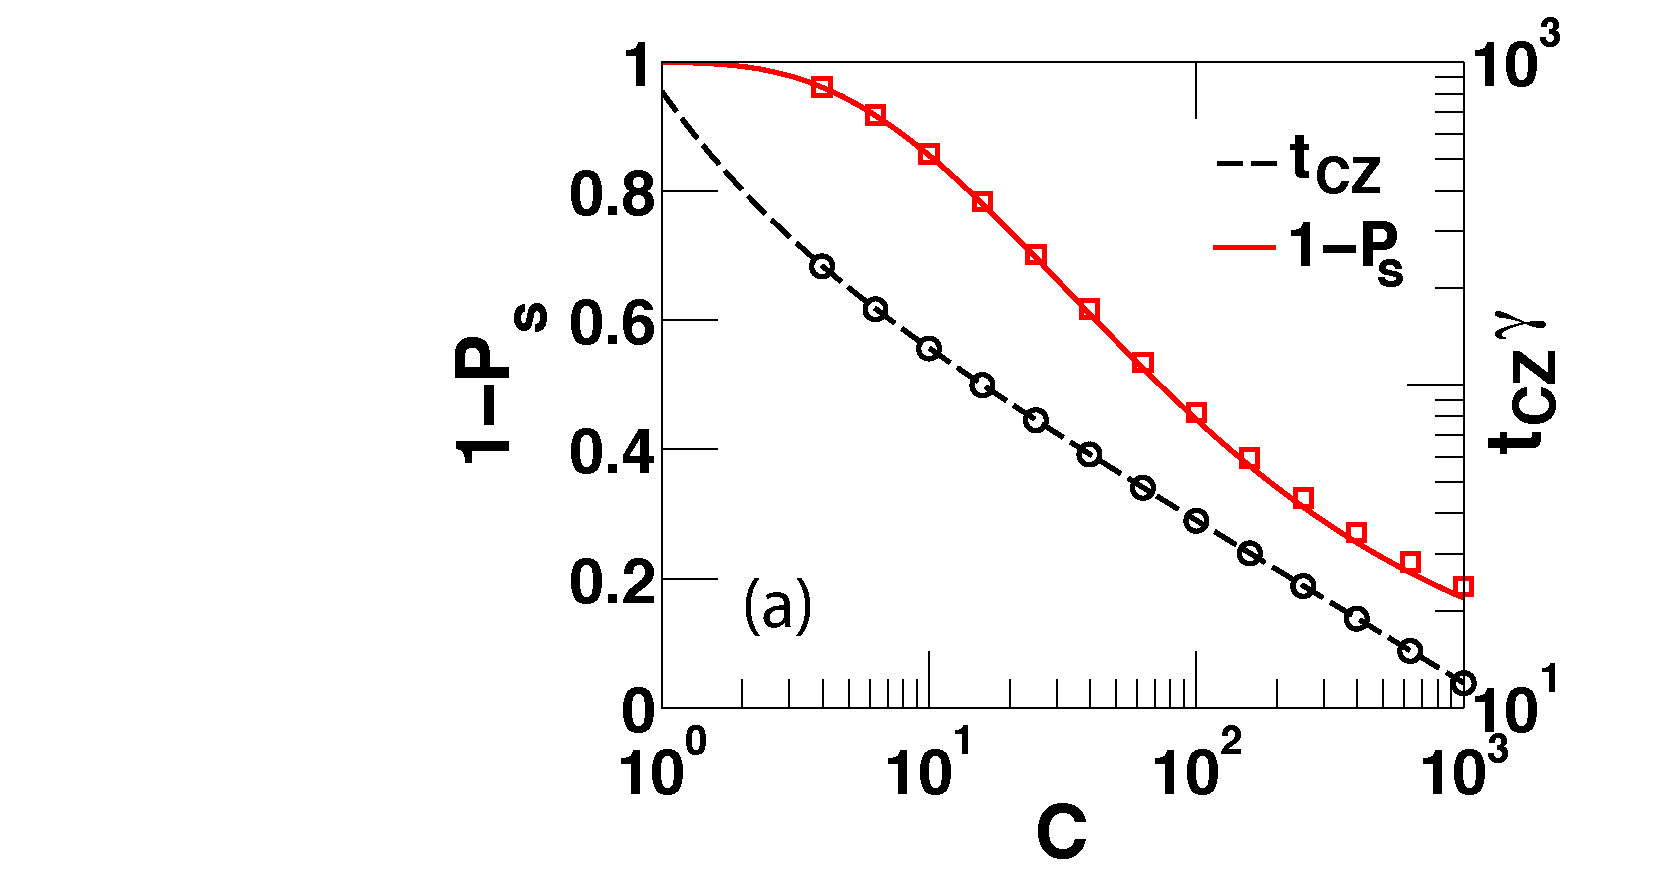
\includegraphics[width=0.45\textwidth]{./figs_Borregaard_PRL2015/figure3a}}}$
\quad\quad
$\vcenter{\hbox{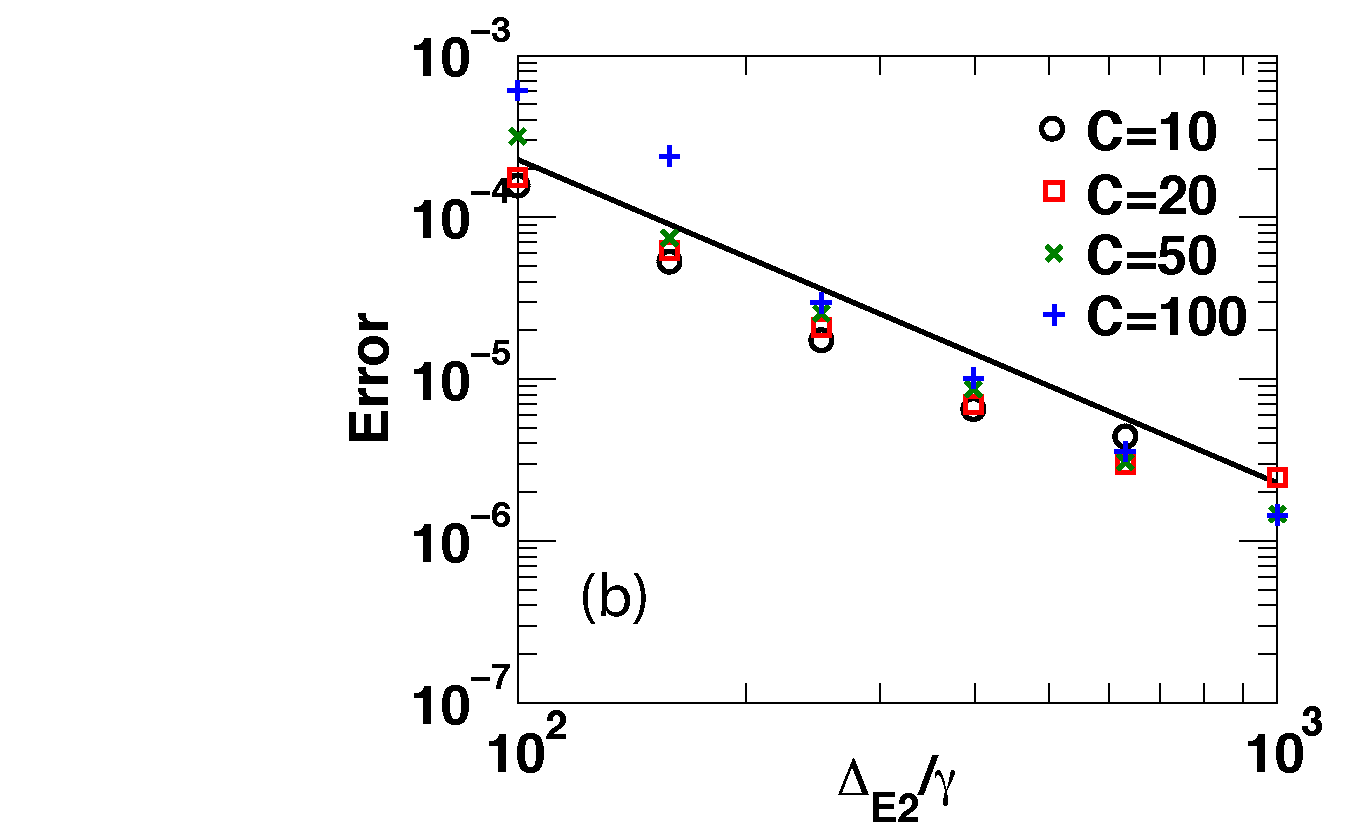
\includegraphics[width=0.45\textwidth]{./figs_Borregaard_PRL2015/figure3b2}}}$
\caption[]
{(a) Failure probability ($1-P_{s}$ - left axis) and gate time ($t_{\text{CZ}}$
-right axis) as a function of the cooperativity ($C$) for the CZ gate. The gate
time is in units of the inverse linewidth $1/\gamma$ of the qubit atoms. We have
assumed a driving of $\Omega=\sqrt{C}\gamma/4$. (b) Gate error as a function of
the detuning $\Delta_{E2}$ in the two-photon-driven CZ-gate for $C=10,20,50$,
and $100$. We have assumed that $\Omega_{\text{\text{MW}}}=4\gamma C^{1/4}$ and
that $\gamma_{g}=\gamma$. The gate error decreases as
$\gamma^{2}/\Delta_{E2}^{2}$ and is independent of $C$.  We have assumed
$\Omega\sim\Delta_{E2}/8$ resulting in a gate time $\sim400/\gamma$.
Solid/dashed lines are analytical results and symbols are numerical simulations
(see Appendix \ref{app:Borregaard_PRL2015}). For both plots, we have assumed
$\kappa=100\gamma$.}
\label{fig:prob}
\end{figure} 

\section{Additional errors}

So far, we have assumed a model where there is no decay from
$\ket{E}\to\ket{g}$. In real atoms, there will, however, always be some decay
$\ket{E}\to\ket{g}$ with a decay rate $\gamma_{g}>0$. The result of such an
undetectable decay is that both the CZ-gate and the Toffoli gate will have an
error $\sim \gamma_{g}/(\gamma\sqrt{C})$. To make this error small, it is thus essential to suppress the
branching ratio $\gamma_{g}/\gamma$. Below we show how to suppress $\gamma_{g}$ by driving the $\ket{g}\to\ket{E}$
transition with a two photon process. As a result, we realize a CZ gate with an
error arbitrary close to zero and a Toffoli gate with an error scaling  as $1/C$
even for a realistic atomic system.

Specifically we think of a level structure for the auxiliary atom, shown in
\reffig{fig:control},
\begin{figure} 
\centering
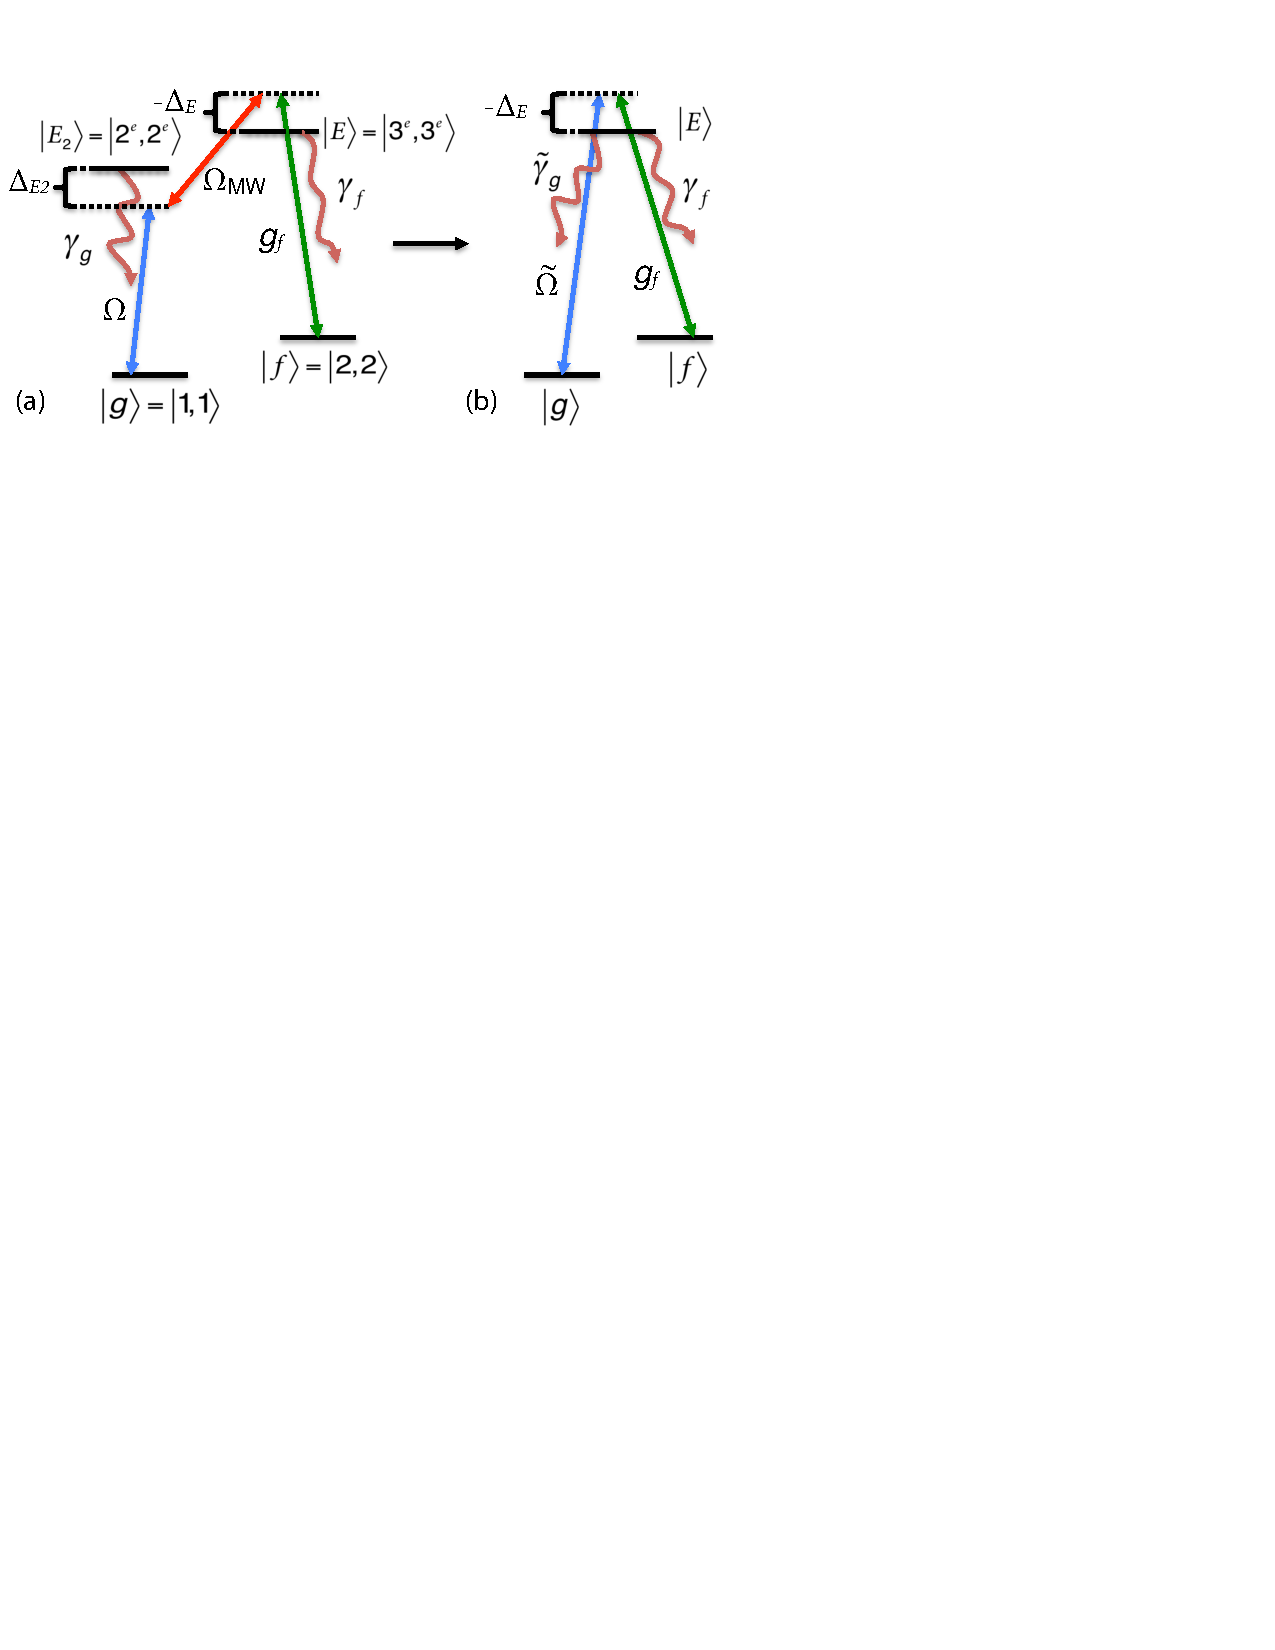
\includegraphics[width=0.75\textwidth]{./figs_Borregaard_PRL2015/figure4}
\caption
[Level structure of auxiliary atom]
{(a) Level
structure of the auxiliary atom and the transitions driven by a weak laser ($\Omega$), a microwave field ($\Omega_{\text{MW}}$) and the cavity ($g_{f}$). We assume that
$\ket{E}\leftrightarrow\ket{f}$ is a closed transition and, for simplicity, we
also assume that $\ket{E_{2}}\leftrightarrow\ket{g}$ is a closed transition but
this is not a necessity. Here $\ket{r^{(e)},r^{(e)}}$ with $r=1,2,3$ refers to
how the atom may be realized in the $(5^{2}P_{3/2})$ states
$\ket{F^{(e)}=r,m^{(e)}=r}$ $5^{2}S_{1/2}$ of Rb${}^{87}$. (b) Effective
three-level atom realized by mapping the two-photon drive to give an effective
decay rate $\tilde{\gamma}_{g}$ and an effective drive $\tilde{\Omega}$. }
\label{fig:control}
\end{figure} 
where we still assume $\ket{E}\leftrightarrow\ket{f}$ to be a closed transition.
For simplicity, we have also assumed $\ket{E_{2}}\leftrightarrow\ket{g}$ to be a
closed transition. Such a level structure could,
e.g. be realized in  ${}^{87}$Rb  as shown in \reffig{fig:control}.  We assume
that a microwave field couples the two excited states such that we can have a
two photon transition from $\ket{g}\to\ket{E}$ and that $\Omega$ is small,
allowing for a perturbative treatment of the coupling. Thus we can map
the system to a simple three-level atom with levels $\ket{g},\ket{E}$ and
$\ket{f}$ and a decay rate $\tilde{\gamma}_{g}$ and drive $\tilde{\Omega}$
between $\ket{g}$ and $\ket{E}$, determined by the two photon driving process as
shown in \reffig{fig:control}. The dynamics are thus similar to what we have
already described for the simple three level atom except that we have the extra
decay $\tilde{\gamma}_{g}$ that introduces an error in the gates
$\sim(\tilde{\gamma}_{g}/\gamma)/\sqrt{C}$, as previously described. In the
limit $C\gg1$, we find
$\tilde{\gamma}_{g}/\gamma\sim\frac{\gamma_{g}\Omega_{\text{MW}}^{2}}{4\gamma\Delta_{E2}^{2}}$.
Thus by increasing $\Delta_{E2}$, we can in principle make these errors
arbitrarily small. The error of the CZ-gate for different $\Delta_{E2}$ is shown
in \reffig{fig:prob}, assuming an initial state of
$(\ket{0}+\ket{1})^{\otimes 2}$. Note that in order to prevent an increasing
scattering probability of level $\ket{E2}$, we need to have $\Omega_{MW}\propto
C^{1/4}$ resulting in a gate error that is independent of the cooperativity, see
Appendix \ref{app:Borregaard_PRL2015}.
The success probability and time of the gates are the same as before with
$\Omega\to\tilde{\Omega}\sim\frac{\Omega_{\text{MW}}\Omega}{2\Delta_{E2}}$. With
similar considerations about the validity of our perturbation as
before, we find that for realistic parameters, we can use $\Omega=\Delta_{E2}/8,
\Omega_{\text{MW}}\sim4\gamma C^{1/4}$ resulting in a gate time of $\sim10$
$\mu$s for typical atomic decay rates and $C\lesssim1000$, see Appendix
\ref{app:Borregaard_PRL2015}.

\section{Possible implementation}

As an example implementation, we consider ultra-cold ${}^{87}$Rb atoms coupled
to nanophotonic cavities~\cite{thompson,Tiecke}. There are some additional
errors originating from the extra states in the ${}^{87}$Rb atoms in this case.
In Appendix \ref{app:Borregaard_PRL2015}, we treat these errors and find that with a detuning of
$\Delta_{E2}=100\gamma$ and a cooperativity of $C\approx100$, a heralded CZ gate
with $\sim67\%$ success probability and a heralded error of $\approx 10^{-3}$
can be realized in $\approx10$ $\mu$s time. This justifies neglecting atomic
decoherence which is typically much slower.
Alternatively the gate can be implemented with atom-like solid-state qubits such
as NV and SiV centers in diamond~\cite{phystoday}. These systems can exhibit
closed transitions and long-lived electronic spin states which are the essential
requirement for the gate~\cite{togan}, while high cooperativities are possible
in  diamond nanocavities~\cite{burek}. A particular advantage of such system is
the long-lived nuclear spin degrees of freedom, which allows each of the color
centers  to act as a multi-qubit quantum network node~\cite{maurer}.   By
entangling electronic spins via the heralded gate, a high-fidelity, fully
deterministic gate can subsequently be performed on qubits stored in nuclear
spins~\cite{Anders2prl}.

\section{Application}

As a particular application, we consider a quantum repeater where entanglement
is first created in small segments (links), which are subsequently connected
using entanglement swapping~\cite{briegel}. By organizing the repeater in a tree
structure, the probabilistic nature of the gate can be efficiently circumvented.
The success rate of distributing entanglement across the total distance L,
scales as $\sim (L/L_{0})^{1-\log_{2}(3/p)}$, where $p<1$ is the success
probability of the swap, $L$ is the total distribution distance and $L_{0}$ is
the length between the links~\cite{Borregaard2015b} (note that in the limit $p\to1$,
the above expression underestimates the rate, e.g., for $p=1$ the actual rate is
$\sim3$ times faster for 128 links). This is a substantial improvement over
direct transmission where the success rate scales exponentially with $L$. For a
realization with nuclear spin memories where the swap can be performed
deterministically the rate can scale even better as
$\sim\log_{2}(L/L_{0})^{-1}$. In order to maintain the favorable scaling without
resorting to time consuming purification, the total number of links,
$N_{\text{max}}$ should be kept below
$N_{\text{max}}\sim-\ln(F_{\text{final}})/(\epsilon_{0}+\epsilon_{g})$, where
$F_{\text{final}}$ is the required fidelity of the final distributed pair and
$\epsilon_{0},\epsilon_{g}\ll1$ are the errors of the initial entanglement
generation and the entanglement swapping respectively. Thus, it is essential
that the errors are kept small, which can be obtained with the heralded gate.

\section{Conclusion}

In conclusion, we have introduced a heralded two-qubit quantum
gate with a conditional fidelity arbitrarily close to unity and an $N$-qubit Toffoli gate
with an error scaling as $1/C$. The gates have a
built-in error detection process, which removes the necessity of extracting the
error by the more complicated process of entanglement purification or quantum
error correction. Our gate is designed for the specific case of optical
cavities, and allows exploiting realistic systems for quantum communication, even though the error rate would inhibit this with deterministic gates. Similar
advantages can be realised in other systems such as those based on circuit QED, where certain errors could be
heralded and thus alleviate the daunting requirements of fault tolerant
computation. 
          
\chapter{Remote entanglement distribution using individual atoms in
cavities}
\label{ch:Borregaard_PRA2015}
%From \cite{Borregaard2015b}
%%%%%%%%%%%%%%%%%%%%%%%%%%%%%%%%%%%%%%%%%%%%%%%%
 

\section{Introduction}

Distribution of entanglement is an essential task in quantum
communication~\cite{kimble,cirac, acin}.  Entanglement can be used to make
highly secure communication channels due to the sensitivity of entangled quantum
systems to external influences~\cite{scarani}. While this sensitivity makes it
possible to detect any attack from an eavesdropper, it also makes it hard to
distribute entanglement over large distances since any noise from the
environment quickly destroys the entanglement. Direct transmission of a quantum signal
suffers from loss and decoherence from the transmission channel, which results
in an exponential decrease of the rate with distance~\cite{briegel}. To overcome
this problem, it has been proposed to use quantum repeaters, where entanglement
is first created over short distances by direct transmission and then stored in
quantum memories until it can be swapped to larger
distances~\cite{briegel,duan3} (See \reffig{fig:figure1}). Much effort has been
devoted to the construction of quantum repeaters based on atomic ensembles,
where the large number of atoms, in principle, enables highly efficient quantum
memories~\cite{sangouard3,cell}. Nonetheless, the limited efficiencies
demonstrated in current experiments with atomic
ensembles~\cite{sangouard3,hammerer} prevents the construction of a practical
quantum repeater based on currently existing setups. 

Single emitter systems such as color centers and trapped ions have also been
considered for quantum repeaters~\cite{childress,sangouard2}. The long coherence
times demonstrated with, e.g. trapped ions make them desirable as quantum
memories. Nonetheless, entanglement needs to be created non-locally between two
memories in the initial step of a repeater. This requires efficient transfer of
information from the quantum memories onto light in the form of single photons.
To this end, it is an advantage to place the emitter inside a cavity, which can
greatly enhance the light-emitter coupling~\cite{acin,ritter}. Entanglement
swapping can then be performed with a cavity mediated CNOT gate
~\cite{pellizari,haroche1} but in this case, the detrimental effect of cavity loss
and spontaneous emission from the emitters may prevent obtaining efficient
entanglement swapping. The parameter characterizing the effect of dissipation in
the emitter-cavity system is the cooperativity, $C$. It has been argued that a
direct implementation of gates in a cavity will make the gate fidelity, $F$,
have a poor scaling of $1-F\sim 1/\sqrt{C}$ \cite{kastoryano,Anders2prl}. To
overcome this problem for current cavities with limited $C$, it has been
suggested to employ entanglement purification after each swap operation to boost
the entanglement but this either requires a large number of resources or a time
consuming sequential generation of purification
pairs~\cite{bennett,deutsch,duan4,pan}.

Here we analyze and compare a number of cavity-based quantum repeaters which
combines various proposals for entanglement generation and cavity-assisted CNOT
gates. We find that the best scheme is where high-fidelity entanglement is
generated using a two-photon detection scheme similar to Ref.~\cite{kimble2} and
swapped to large distances using the heralded CZ-gate proposed in
Ref.~\cite{Borregaard2015a}. The heralded gate enables nearly perfect entanglement
swapping when successful allowing for many swaps without the need of
entanglement purification. As a result, high-rate entanglement distribution is
achieved even for low cooperativities.

Compared to the other cavity-based repeaters, this high-fidelity repeater
achieves up to two orders of magnitude higher secret key rate (see below) for
realistic parameters and large distances ($1000$ km). Specifically, we have
compared to repeaters where entanglement is generated using a single-photon
detection scheme similar to Ref.~\cite{huelga}, which allows for a better rate
at the expense of fidelity. Furthermore, we have considered schemes where
entanglement swapping is achieved using the deterministic CNOT gate suggested in
Ref.~\cite{Anders2prl}, combining it with the local entanglement generation
scheme of Ref.~\cite{Anders1prl}. The advantage of this gate is that the
fidelity scales as $1-F\sim 1/C$, which is a significant improvement from the
$1/\sqrt{C}$ scaling, characterizing the performance of a direct implementation
of gates in a cavity. As a result, long-distance entanglement distribution can
also be achieved with this gate but it requires cooperativities above $100$,
which might be challenging to achieve experimentally. Furthermore, we include
the possibility of initial purification in repeaters based on the single-photon
detection scheme in order to allow for the higher rate of this scheme to
compensate for the lower fidelity compared to the two-photon detection scheme.

To reflect a realistic near-term approach to quantum repeaters, we only consider
scenarios with 2 or 4 qubits per repeater station. For the same reason, we also
do not consider the possibility of intermediate entanglement purification. Here,
initial purification refers to purification in the elementary links (see
\reffig{fig:figure1}) while intermediate purification refers to purification in
the subsequent stages of a repeater. We have numerically optimized all the
considered repeater schemes for a range of cooperativities and distances to find
the highest achievable secret key rate (see below). Note that a similar
optimization of repeater schemes based on dynamical programming was described in
Ref.~\cite{jiang2007}. In that work, both initial and intermediate entanglement
purification was considered assuming high-fidelity operations.  Our optimization
is less detailed since we do not consider intermediate purification. On the
other hand, we include how the errors of the operations depend on the physical
parameters such as the cooperativity and investigate concrete physical
implementations.
Finally, we compare the high-fidelity repeater considered here to both an
ion-trap repeater and one of the best repeaters based on atomic
ensembles~\cite{sangouard3}. For a distance of 1000 km, the high-fidelity
repeater outperforms both of these schemes for $C\gtrsim30$.

\section{High-fidelity quantum repeater}  \label{sec:generation}

We will first describe the details of the high-fidelity quantum repeater, which
we find to have the best performance and later discuss and compare with the
various other schemes. The first step in any quantum repeater is to create
non-local entanglement in the elementary links (see \reffig{fig:figure1}).
\begin{figure} 
\centering
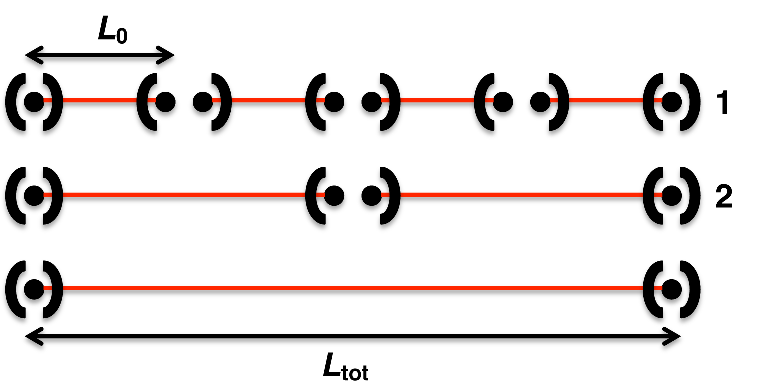
\includegraphics[width=4.0in]{./figs_Borregaard_PRA2015/figure1}
\caption
[The general architecture of a quantum repeater]
{The general architecture of a quantum repeater. The total distance,
over which entanglement should be distributed, is divided into elementary links
of length $L_{0}$ connected by repeater stations pictured as cavities containing
single emitters. After creating entanglement in the elementary links, the
entanglement is swapped to larger distances by combining the elementary links.
The numbers to the right in the figure refers to the swap level of the repeater.
In the first swap level, the four elementary links are connected pairwise to
make two longer links. In the second swap levels these two links are connected
to create entanglement over the total distance. The total number of swap levels
is thus 2 for this depicted setup. }
\label{fig:figure1}
\end{figure} 
To this end, a two-photon detection scheme, as proposed in Ref.~\cite{kimble2},
is considered. The basic setup is shown in \reffig{fig:figure2}(a).
\begin{figure} 
\centering
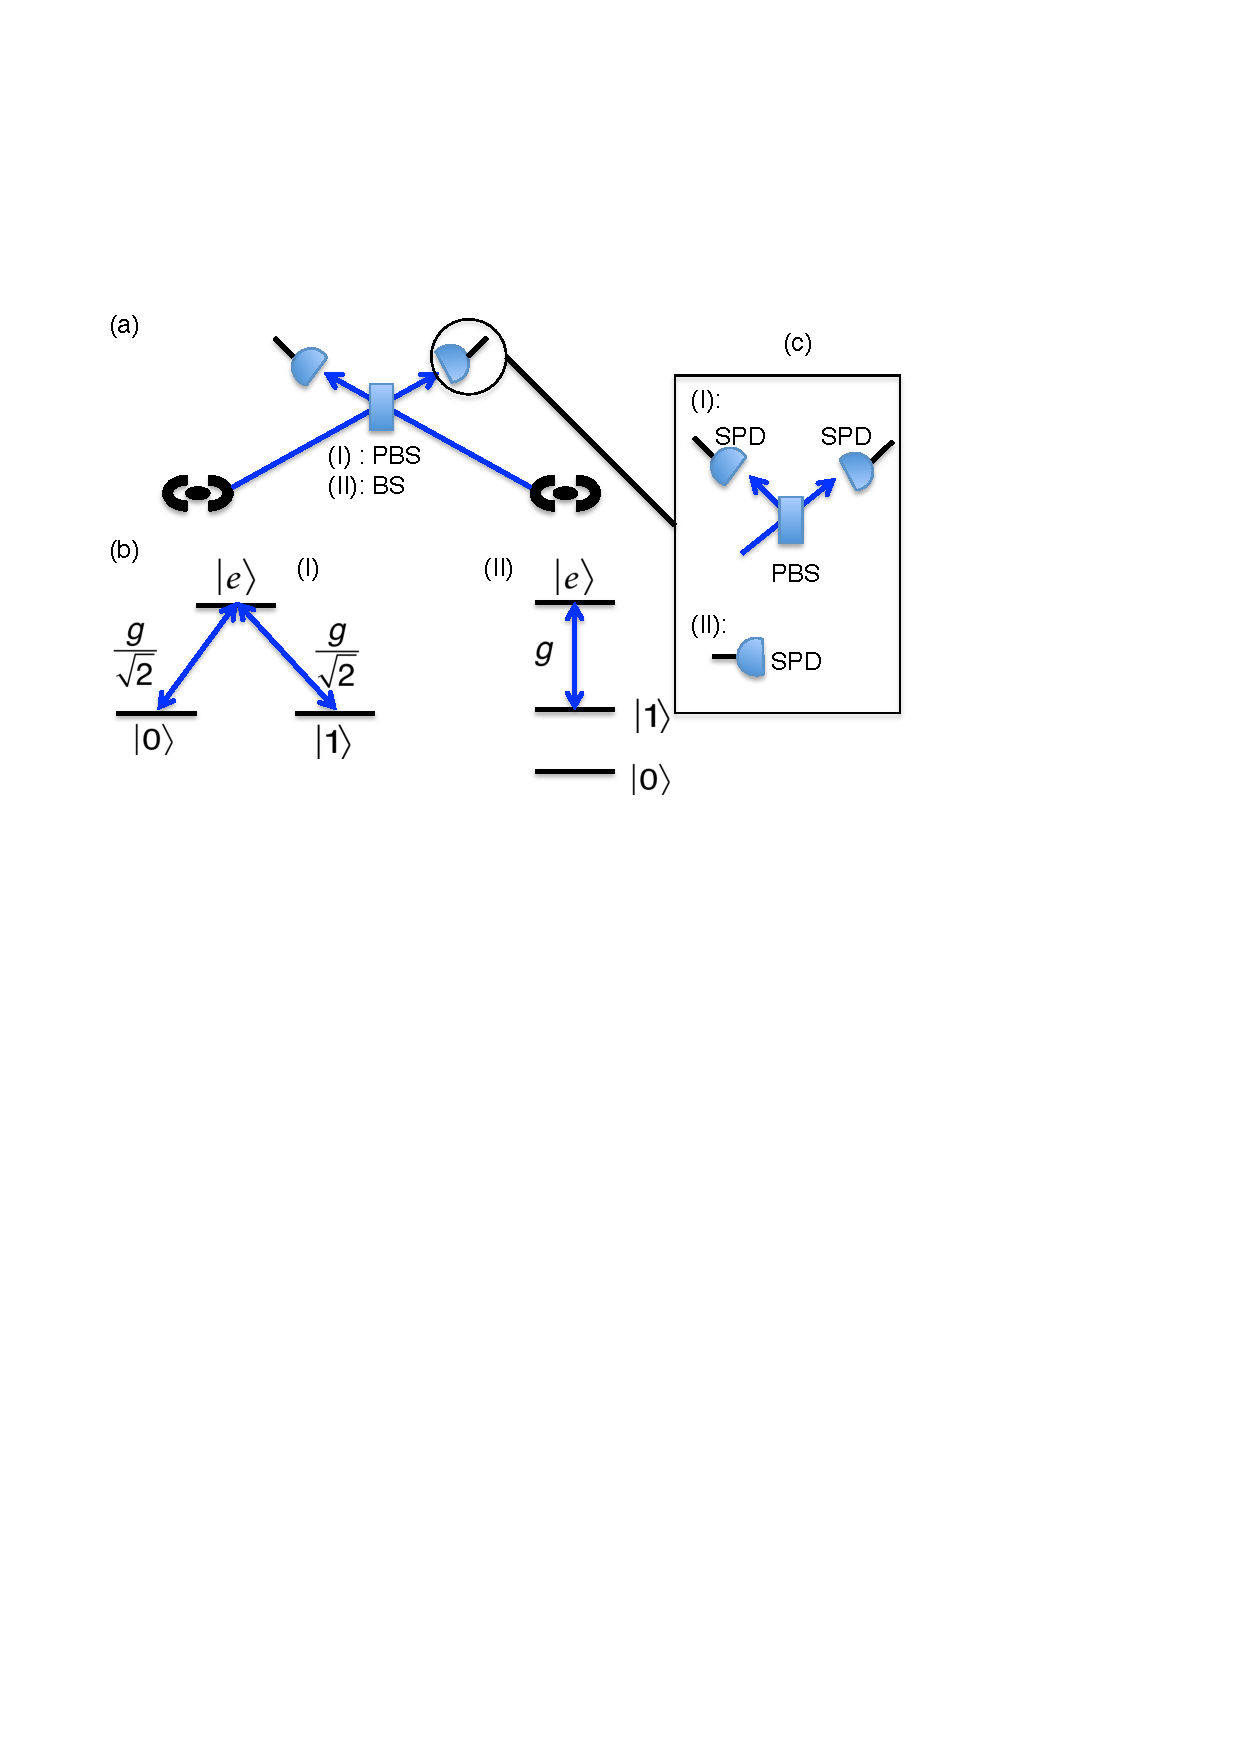
\includegraphics[width=0.7\textwidth]{./figs_Borregaard_PRA2015/figure2}
\caption[Entanglement generation]{Entanglement generation in the elementary
links where emission from two cavities are combined on a beam splitter. (a)
shows the basic setup, (b) shows the level structure of the emitters and (c)
shows the detection setup.  (I) refers to the two-photon detection scheme and
(II) refers to the single-photon detection scheme. Both schemes use a central
station with either (I) three polarizing beam splitters (PBS) and four
single-photon detectors or (II) a single balanced beam splitter (BS) and two
single-photon detectors.  $g$ denotes the cavity coupling. For the two-photon
scheme the levels $\ket{0}$ and $\ket{1}$ are assumed to have equal coupling of
$g/\sqrt{2}$ to the excited state $\ket{e}$.}
\label{fig:figure2}
\end{figure} 
Both emitters are initially prepared in the excited state $\ket{e}$ by a strong
excitation pulse and the cavity is assumed to couple both the
$\ket{e}\to\ket{1}$ and $\ket{e}\to\ket{0}$ transitions with equal coupling
strength $g/\sqrt{2}$ (see \reffig{fig:figure2}(b)). The two transitions are,
however, assumed to produce photons with different polarizations such that the
emission of a cavity photon creates an entangled state between the photon and
the emitter of the form
$\frac{1}{\sqrt{2}}\left(\ket{0}\ket{1_{1}}_{L}+\ket{1}\ket{1_{2}}_{L}\right)$
where $\ket{1_{1}}_{L}$ ($\ket{1_{2}}_{L}$) is the single photon state with
polarization 1 (2). The probability of one of the emitters to emit a photon of
either polarization through the cavity, into an optical fiber transmitting it to
the detection stage during a time interval $[0;T]$ is
\begin{equation} \label{eq:phot1}
P_{\mathrm{phot}}=\frac{4C}{1+4C}\left(1-e^{-\gamma(1+4C)T}\right), 
\end{equation} 
assuming perfect outcoupling to the fiber and that the decay rate of the cavity,
$\kappa$, is much larger than the cavity coupling, $g$. We have here introduced
the cooperativity $C=g^{2}/\kappa\gamma$, where $\gamma$ is the spontaneous
emission rate of the emitters into modes other than the cavity. This is the key
parameter characterizing the performance of the cavity-based repeaters. The
photons are sent from the cavities to a central polarizing beam splitter (PBS).
If two photons of the same polarizations are incident on the PBS, they leave in
different output ports, while photons of different polarization leave in the
same output port. The outputs are then sent to a second set of polarizing beam
splitters and all four outputs of these are finally measured with single photon
detectors (SPD). A click in a detector in each arm heralds the creation of the
Bell state $\ket{\Phi^{+}}=(\ket{00}+\ket{11})/\sqrt{2}$ between the emitters up
to a local qubit rotation. Neglecting dark counts of the detectors, the heralded
fidelity is unity (see App.~\ref{two}) while the success probability of the
scheme is $P_{\mathrm{2click}}=\frac{1}{2}\eta^{2}P_{\mathrm{phot}}^{2}$ with $\eta$
being the total detection efficiency including inefficient outcoupling of the
cavity light, losses in the transmission fibers and imperfect detectors.
Compared to schemes based on single-photon detection (see below) the rate of
this two-photon detection scheme decreases rapidly with decreasing $\eta$. On
the other hand, it has a high fidelity, which is desirable for the subsequent
stages of entanglement swapping, as we will show below.

For entanglement swapping, we find that the best performance is achieved using
the heralded CZ-gate described in Ref.~\cite{Borregaard2015a}. The gate was described
in detail for ${}^{87}$Rb atoms in Ref.~\cite{Borregaard2015a} but it can be easily
generalized to any set of emitters, which have the appropriate level structure
(see \reffig{fig:figure3}). Note that the gate operation relies on only qubit
state $\ket{1}$ coupling to the cavity while the states $\ket{0}$ and $\ket{1}$
had equal cavity couplings in the entanglement generation scheme. To achieve
this change in couplings, the state $\ket{0}$ should be mapped to another level
in between the entanglement generation and the gate operation. For a realization
with alkali atoms where the qubit states would be realized in the hyperfine
grounds states, this could be achieved by applying a magnetic field to resolve
the hyperfine states and applying a microwave pulse resonant with only the
$\ket{0}$ state.
\begin{figure}
\centering
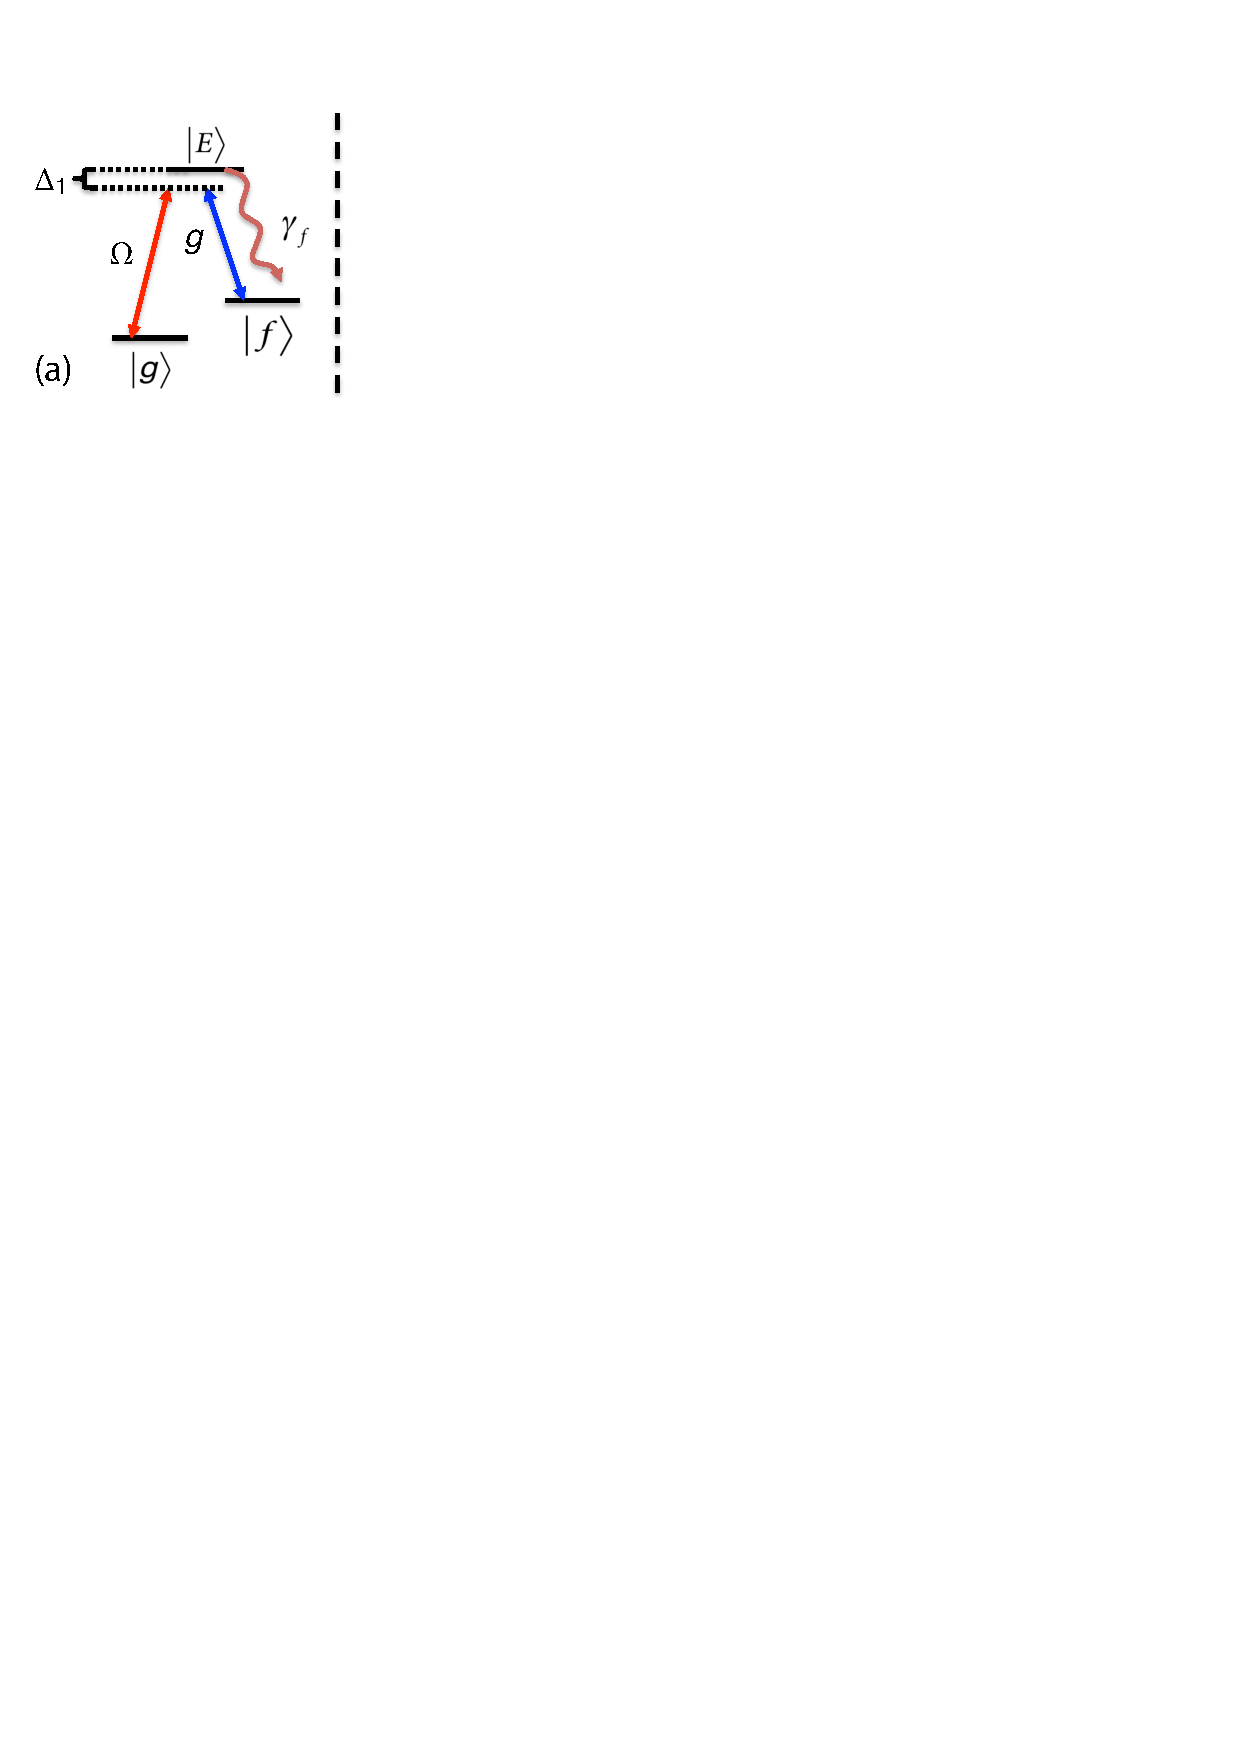
\includegraphics[width=0.3\textwidth]{./figs_Borregaard_PRA2015/figure3a}
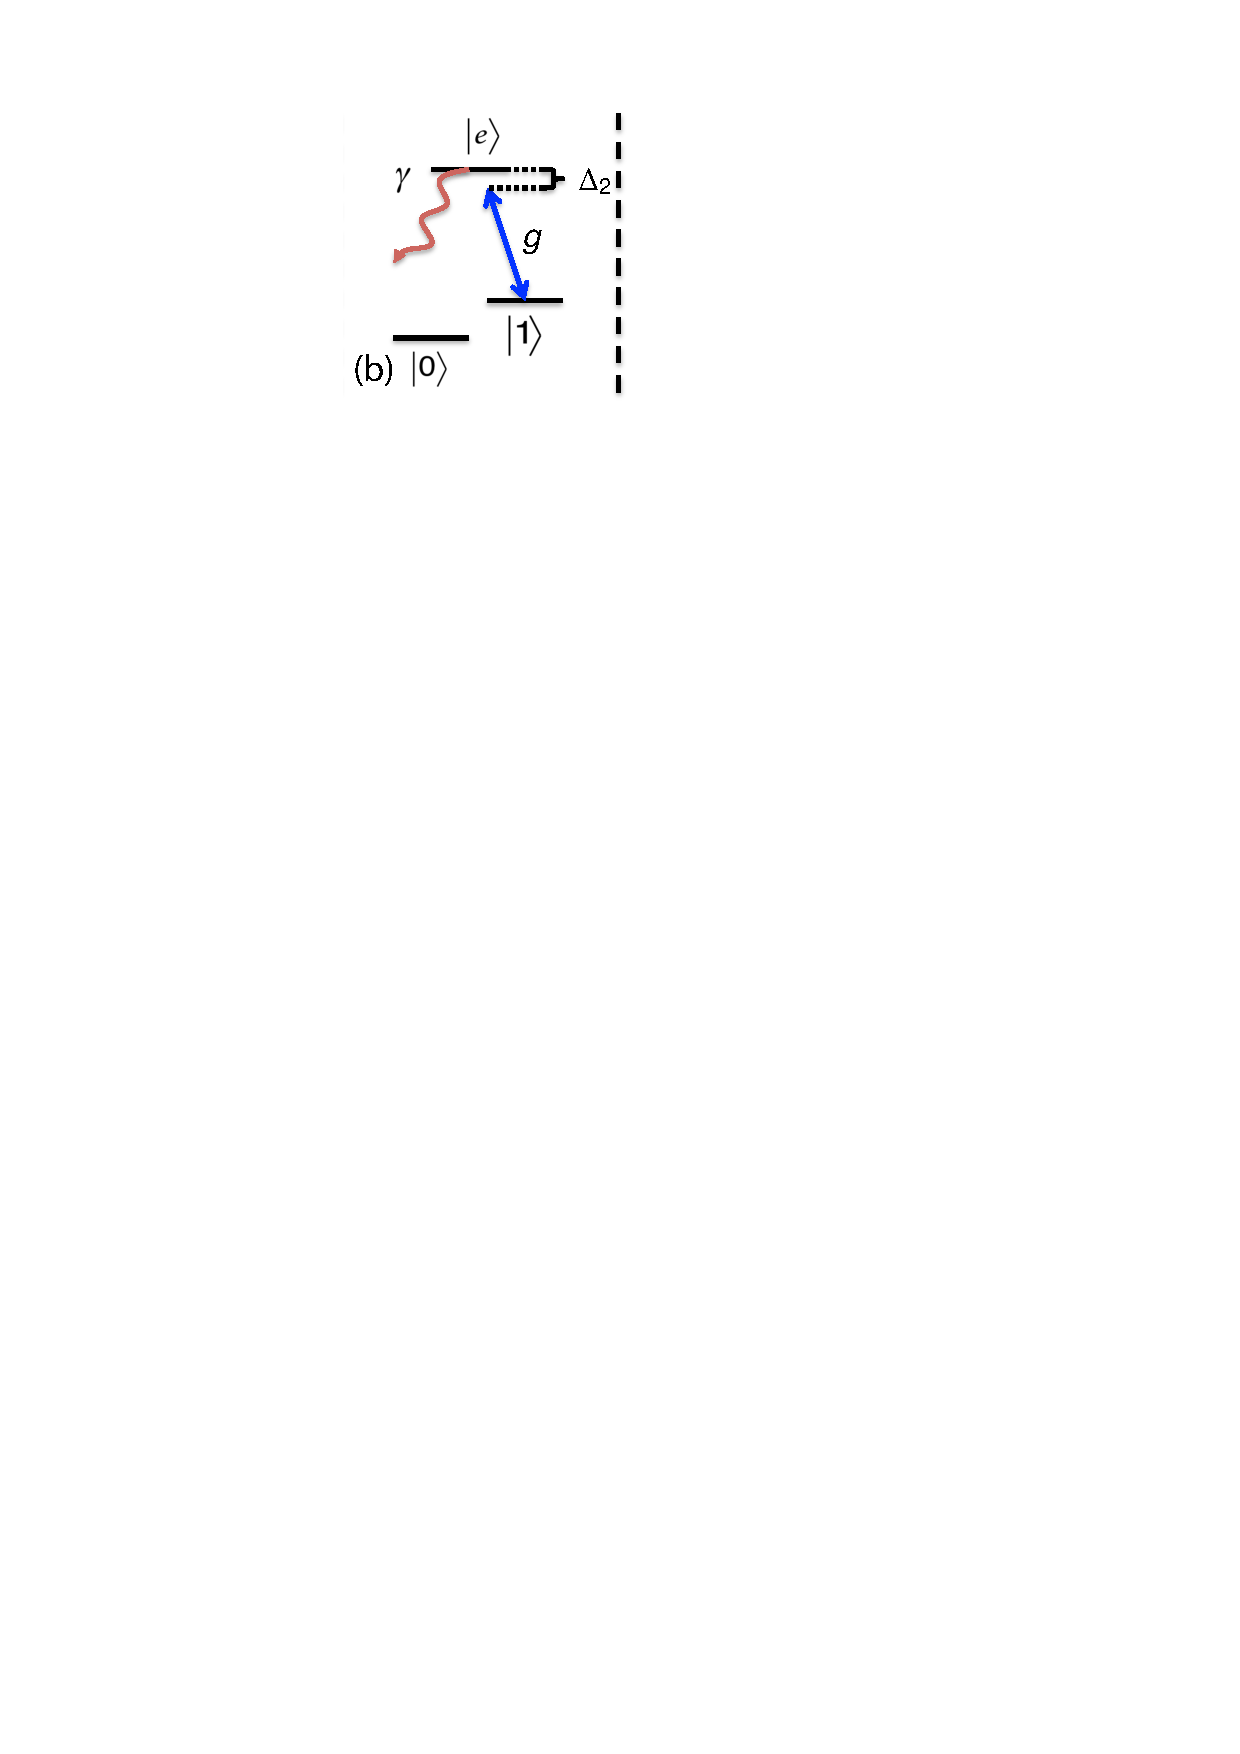
\includegraphics[width=0.3\textwidth]{./figs_Borregaard_PRA2015/figure3b}
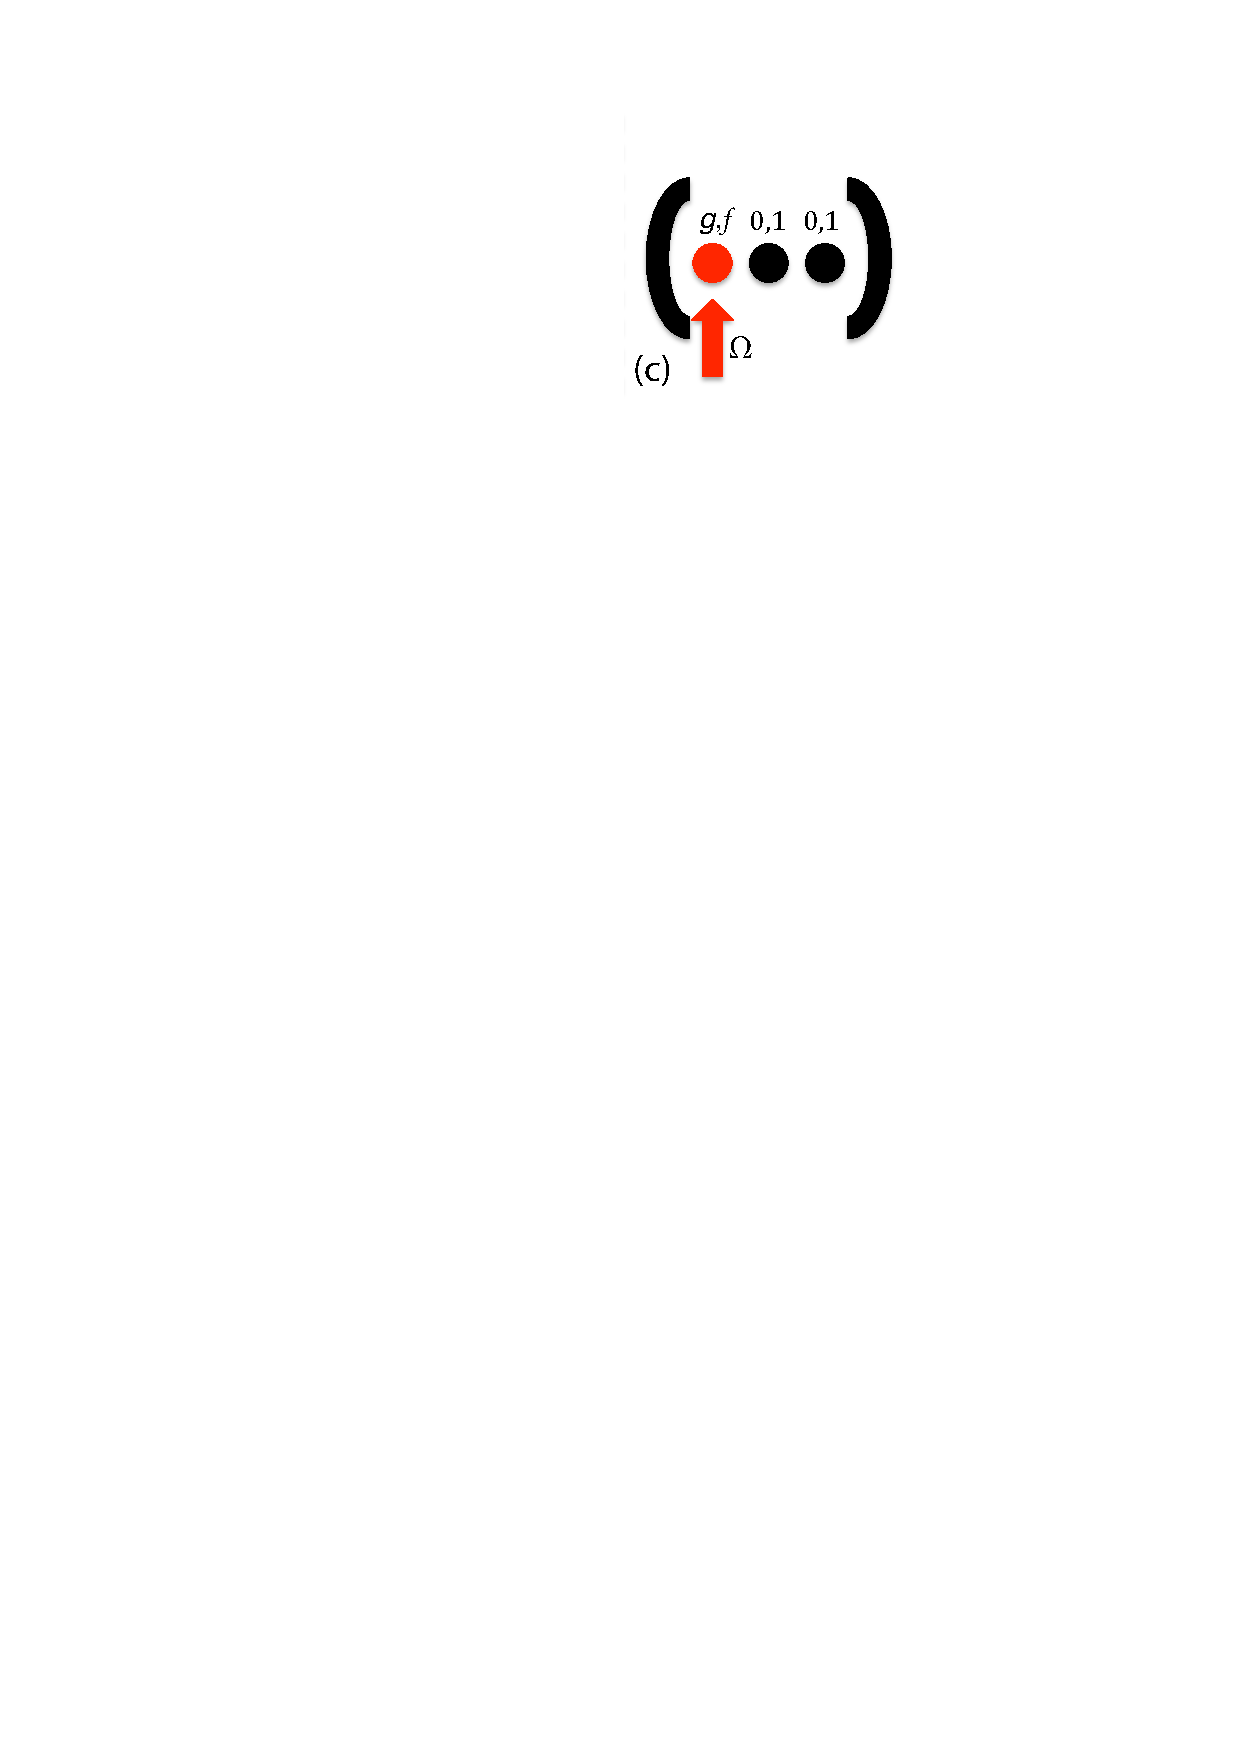
\includegraphics[width=0.3\textwidth]{./figs_Borregaard_PRA2015/figure3c}
\caption
[Schematics of the heralded CZ gate]
{ Schematics of the heralded CZ gate~\cite{Borregaard2015a}. (a) is the level
structure of the auxiliary atom, (b) is the level structure of the qubit atoms
and (c) shows the cavity containing the auxiliary atom and the two qubit atoms.
Assuming that $\ket{E}$ only decays to $\ket{f}$ by e.g. driving the transition
$\ket{g}\to\ket{E}$ with a two photon process, any spontaneous emission or
cavity decay will change the state of the auxiliary atom from the initial state
$\ket{g}$ to $\ket{f}$. The gate is thus conditioned on measuring the auxiliary
atom in state $\ket{g}$ at the end of the gate.}
\label{fig:figure3}
\end{figure}

In the heralded gate, the cavity is assumed to contain two qubit atoms and one
auxiliary atom to facilitate the gate. The auxiliary atom is initialized in a
state $\ket{g}$ that does not couple to the cavity and it would therefore not
interfere with the entanglement generation scheme. By addressing the auxiliary
atom with a weak laser pulse, an AC Stark shift is introduced, which gives a
phase that depends on the state of the qubit atoms. Together with single qubit
rotations, this enables a CZ-gate between the two qubit atoms. Furthermore, the
auxiliary atom can function as an error detector in the sense that any cavity
decay or spontaneous emission changes the state of the atom. Performing a
heralding measurement of the state of the auxiliary atom at the end of the
driving pulse removes all dissipative errors. As a consequence, the gate gets
limited only by non-adiabatic effects. As shown in Ref.~\cite{Borregaard2015a}, a
heralded error below $4\times 10^{-5}$ is possible with a gate time of
$\sim377/(\gamma\sqrt{C})$, where $\gamma$ is the atomic linewidth. The failure
probability of the gate scales as $1/\sqrt{C}$ and the high fidelity thus comes
at the cost of a finite but possibly low failure probability. A CZ gate combined
with single qubit rotations is sufficient to perform direct entanglement
swapping. For simplicity, we assume perfect single qubit rotations and 100\%
efficient measurement of atomic states for all schemes considered. Relaxing this
assumption will in general decrease the rate of all the considered repeater
schemes but schemes with a high number of swap levels, such as the high-fidelity
repeater, will be influenced more on the rate than schemes with a low number of
swap levels.

The advantage of the high-fidelity repeater can be understood by considering the
requirement for reaching a certain threshold fidelity, $F_{\mathrm{final}}$ of the
distributed pair. In this case, the maximum number of swap levels is
$N_\mathrm{max}\sim -\log_{2}(F_{\mathrm{final}}/(\epsilon_{0}+\epsilon_{g}))$,
where $\epsilon_{0},\epsilon_{g}\ll1$ are the errors of the initial entanglement
generation and the entanglement swapping respectively. The combination of the
high-fidelity two-photon detection scheme and the heralded gate thus makes it
possible to have a repeater with many elementary links while maintaining a high
fidelity of the final distributed pair even for low cooperativities since the
error of the heralded gate is still high in this regime.

\subsection{Secret key rate} \label{sec:secret}
We imagine that the distributed entanglement is used to generate a secret key
between two parties referred to as Alice and Bob. There exist various quantum
key distribution schemes \cite{scarani,bennett2,ekert,bruss}, however, the
general idea is that Alice and Bob can exclude that an eavesdropper has any
information about the key by measuring their qubits and comparing results. We
will assume that a six-state version of the BB84 protocol described in Ref.
\cite{bruss} is used to generate the secret key. This protocol consists of three
main steps. First Alice and Bob picks a basis according to some probability
distribution and measure the state of their qubits thereby producing two bit
strings referred to as the \emph{raw key}. Afterwards they compare their choice
of basis and only keep the bits where they chose the same measurement basis
thereby producing a \emph{sifted key}. Finally, Alice and Bob estimate the
information that some eavesdropper could possibly have obtained about their key
and perform privacy amplification \cite{scarani}. If the errors are not too big,
they can obtain a shorter but completely secure key.  For the six-state
protocol, the secret key rate, $r_{\mathrm{secret}}$ can be defined as
\begin{equation}
r_{\mathrm{secret}}=r_{\mathrm{dist}}p_{\mathrm{sift}}f_{\mathrm{secret}},
\end{equation}
where $r_{\mathrm{dist}}$ is the distribution rate of the entangled pairs,
$p_{\mathrm{sift}}$ is the probability that Alice and Bob choose the same
measurement basis and $f_{\mathrm{secret}}$ is the secret key fraction, which
depends on the fidelity of the distributed pairs. We assume a worst case
scenario where the distributed pairs are Werner states of the form
\begin{eqnarray}
\rho&=&F\ket{\Phi^{+}}\bra{\Phi^{+}} +
\frac{1-F}{3}\Big(\ket{\Phi^{-}}\bra{\Phi^{-}}
+\ket{\Psi^{+}}\bra{\Psi^{+}}+\ket{\Psi^{-}}\bra{\Psi^{-}}\Big).
\end{eqnarray}
For such states, it is shown in Ref. \cite{scarani} that the secret key fraction
in the six-state protocol can be estimated in the limit of infinitely long raw
keys to be
\begin{equation} \label{eq:secret2}
f_{\mathrm{secret}}=1-h(\epsilon)-\epsilon+(1-\epsilon)
h\left(\frac{1-3\epsilon/2}{1-\epsilon}\right),
\end{equation} 
where $\epsilon=2(1-F)/3$ and
$h(p)=-p\mathrm{log}_{2}(p)-(1-p)\mathrm{log}_{2}(1-p)$ is the binary entropy.
Eq.~\eqref{eq:secret2} is valid in the limit of perfect sifting and privacy
amplification, which we assume to be the case. Furthermore, we assume an
asymmetric version of the six state protocol, where one basis is used almost all
the time such that $p_{\mathrm{sift}}\approx1$ \cite{scarani}.
\reffig{fig:figure5} shows how the secret key fraction depends on the fidelity
of the distributed pairs.
\begin{figure} 
\centering
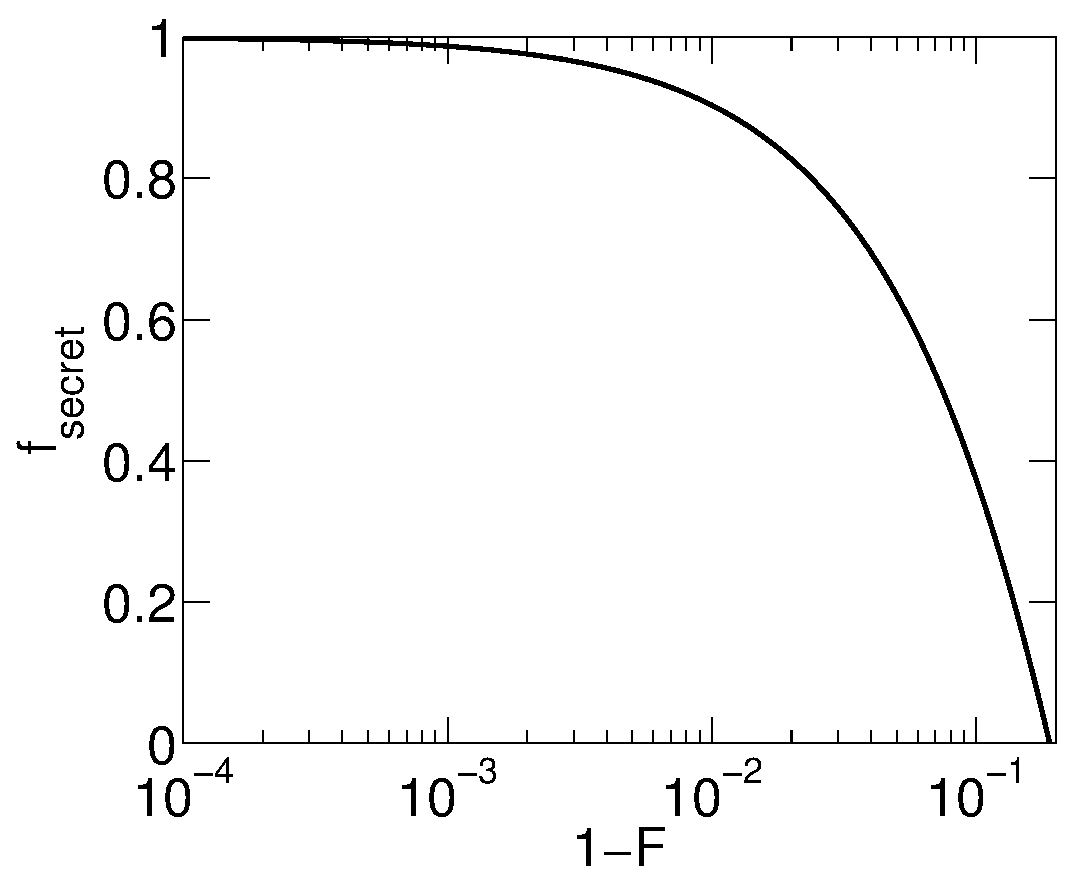
\includegraphics[width=0.6\textwidth]{./figs_Borregaard_PRA2015/figure5}
\caption[Secret key fraction]{Secret key fraction ($f_{\mathrm{secret}}$) as a
function of the infidelity, $1-F$, of the final entangled pair. For
$1-F\gtrsim19 \%$ it is no longer possible to extract a secret key from the raw
keys.}
\label{fig:figure5}
\end{figure} 
As shown in the figure, high-fidelity pairs are required in order to have a
non-vanishing secret key fraction. Again, this points to the high-fidelity
two-photon detection scheme and the nearly error-free heralded entanglement
swapping as the best choice for the repeater.

\subsection{Repeater architecture}

The main goal of the quantum repeater is to overcome the effect of fiber losses.
We model the fiber losses with a transmission efficiency
$\eta_{\mathrm{f}}=e^{-L_{0}/2L_\mathrm{att}}$, where $L_{0}$ is the length of
the elementary links of the repeater and $L_\mathrm{att}$ is the fiber attenuation
length.
$\eta_{\mathrm{f}}$ enters in the total detection efficiency $\eta$ as described
above. For a given resource of $2^{n}+1$ repeater stations, one can either use
all stations in a single repeater with $n$ swap levels or one can construct a
number of parallel, independently operated chains of repeaters with less swap
levels. Increasing the number of swap levels, decreases the fiber losses in the
elementary links and thus increases the rate of entanglement generation. If,
however, the length of the elementary links is already small,  e.g.
imperfect SPD dominates the rate, then increasing the number of swap levels does
not lead to any improvement. In this case it is advantageous to use the extra
repeater stations to make another repeater with less swap levels, which runs in
parallel with the already existing one. To make a proper assessment of the
performance of repeater one should therefore include that adding swap levels
costs resources in the form of additional repeater stations. In our comparison,
we therefore consider a normalized secret key rate,
$\tilde{r}_{secret}=r_{secret}$/(~\#~of stations), which is the secret key rate
divided by the total number of repeater station instead of the bare secret key
rate. To evaluate the performance of the repeater we calculate the achievable
rate $\tilde r_{secret}$ as described in Appendix~\ref{app:rate} with the
assumptions summarized in \tabref{tab:parameter} about fiber losses etc.. The
resulting rate for various swap level used in the repeater is shown in
\reffig{fig:figureX4} as a function of distance. As seen in the figure, the
optimal number of swap level changes with distance while considering the
normalized secret key rate. The rate was calculated as described in
App.~\ref{app:rate} for a cooperativity of 100 with the assumptions summarized
in \tabref{tab:parameter} about fiber losses, detection efficiencies etc. For
distances $\lesssim 150$ km, only a single swap level is needed since the fiber
losses are relatively small while more swap levels are needed as the distance
increases.

\begin{figure} 
\centering
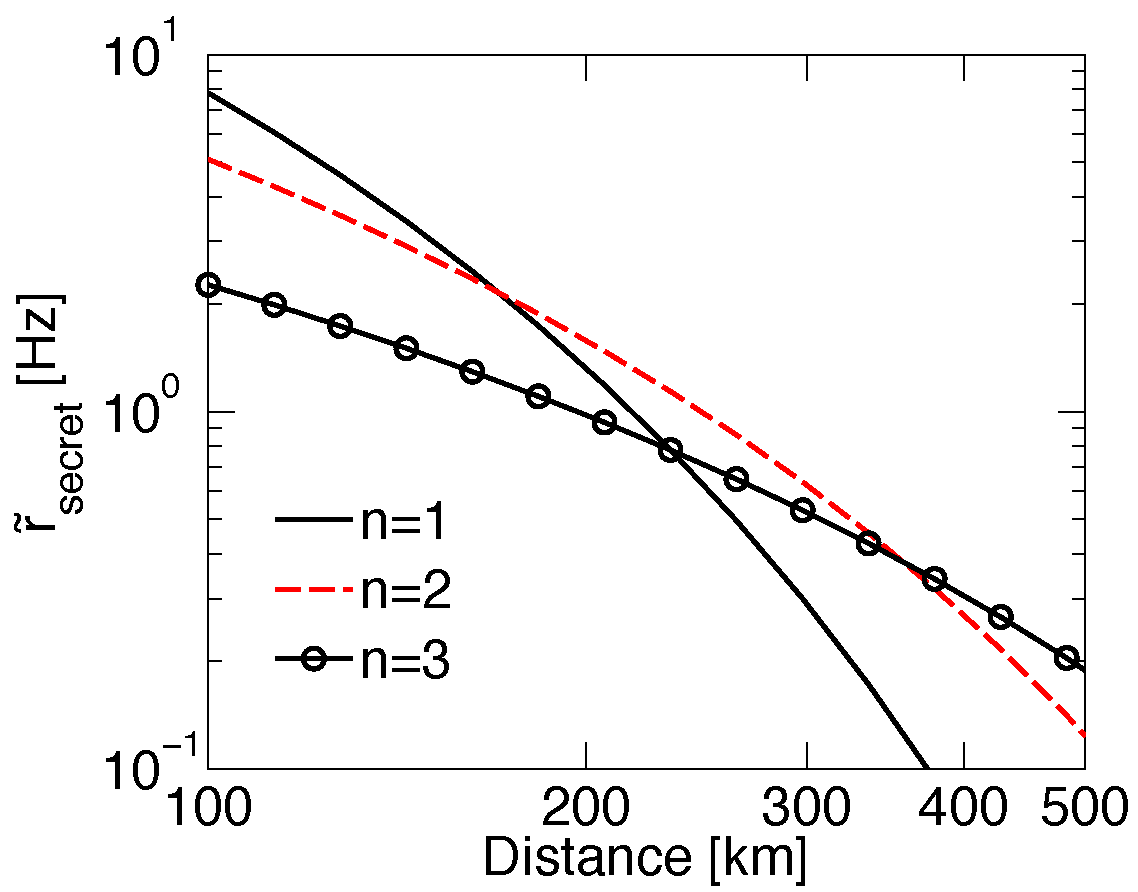
\includegraphics[width=0.65\textwidth]{./figs_Borregaard_PRA2015/figureX4}
\caption[Number of swap levels]{Normalized secret key rate per
station($\tilde{r}_{\mathrm{secret}}$) as a function of the distribution distance
for a high-fidelity repeater consisting of the two-photon entanglement
generation scheme and the heralded gate for entanglement swapping.  We have
considered $n=2,3$ and 4 swap levels and have assumed a cooperativity of $C=$100
and two qubits per repeater station. The secret key rate was calculated as
described in App.~\ref{app:rate} with the assumptions summarized in
\tabref{tab:parameter}.  }
\label{fig:figureX4}
\end{figure} 
  
In most repeater schemes, the qubits in each repeater station are assumed to be
operated simultaneously with half of the qubits being used to generate
entanglement with the neighboring station to each side such that entanglement
attempts in all the elementary links are done simultaneously. We will refer to
this as a \emph{parallel} repeater.  We will, however, also consider another
sequential way of operating the qubits, where all qubits in a station are first
used to make entanglement in one elementary link. After this has been obtained,
all but one qubit are then used to make entanglement over the neighboring link
in the opposite direction. This is referred to as a \emph{sequential} repeater.
The advantage of the sequential repeater is that the rate of the lowest level in
the repeater, the entanglement generation, is increased. This comes at the cost
of a waiting time between entanglement attempts in neighboring links. As the
number of qubits per repeater station increases the sequential repeater will
start to outperform the parallel repeater. We find that this happens with 4
qubits per repeater station (see Sec.~\ref{sec:optim}).

\section{Other cavity based repeaters} \label{sec:other} 

We have found that the high-fidelity repeater that we have described above
outperforms a number of other cavity-based repeater schemes, which can be
constructed with different schemes of entanglement generation and CNOT gates.
Below, we describe the constituents of these other schemes and compare them to
those of the high-fidelity repeater

\subsection{Single-photon entanglement creation} \label{sec:1phot}
It has also been suggested to use single-photon detection schemes similar to
Ref.~\cite{huelga} to generate entanglement in the elementary links. The setup
of a single-photon detection scheme is also shown in \reffig{fig:figure2}. We
assume that the two emitters are initially prepared in a state
\begin{equation}
(1-\epsilon^{2})\ket{00}+\epsilon^{2}
\ket{ee}+\epsilon\sqrt{1-\epsilon^{2}}\left(\ket{0e}+\ket{e0}\right)
\end{equation}    
by a weak excitation pulse such that the excitation probability is
$\epsilon^{2}$. An emitter can then go from state $\ket{e}$ to state $\ket{1}$
by emitting a cavity photon. The emitted photons are collected from the cavities
and combined on a balanced beam splitter (BS) on a central station between the
two cavities. Neglecting losses, the detection of a single photon after the BS
will project the state of the emitters into the Bell state
$\ket{\Psi^{+}}=\frac{1}{\sqrt{2}}\left(\ket{01}+\ket{10}\right)$, up to a
single qubit rotation, in the limit $\epsilon^{2}\ll1$, where we can neglect the
possibility of double excitations. The probability of an emitter to go from
$\ket{e}$ to $\ket{1}$, by emission of a cavity photon during a time interval
$[0;T]$, is $P_{\mathrm{phot}}$ (see Eq.~\eqref{eq:phot1}) under similar
assumptions as in the two-photon scheme described above. Neglecting dark counts
but including losses, the total probability of a single click at the central
station is $P_{\mathrm{1click}}=2\eta
P_{\mathrm{phot}}\epsilon^{2}(1-\epsilon^{2})+(2\eta-\eta^{2})P_{\mathrm{phot}}^{2}\epsilon^{4}$
with $\eta$ being the total detection efficiency as for the two-photon scheme.
The first term is the probability to emit and detect a single photon while the
second term is the probability of emitting two cavity photons but only getting a
single click (we assume that we do not have access to number-resolving
detectors). The probability, to have a single click and have created the state
$\ket{\Psi^{+}}$, is $P_{\mathrm{correct}}=2\eta
P_{\mathrm{phot}}\epsilon^{2}(1-\epsilon^{2})$. The average heralded fidelity
conditioned on a single click is thus
$F_{1}=P_{\mathrm{correct}}/P_{\mathrm{1click}}$. To lowest order in $\epsilon$,
$F_{1}\sim1-(1-\eta/2)P_{\mathrm{phot}}\epsilon^{2}$ while the success probability
is $P_{\mathrm{1click}}\sim2\eta P_{\mathrm{phot}}\epsilon^{2}$. There is thus a
tradeoff set by $\epsilon^{2}$ between the success probability and the fidelity
for the single-photon detection scheme. This is in contrast to the two-photon
detection scheme where $F=1$ regardless of success probability.

The success probability of the single-photon detection scheme is not as
sensitive to the detection efficiency $\eta$ as the two-photon detection scheme
as shown in \reffig{fig:figureX3}.
If the detection efficiency $\eta$ is large, the two-photon scheme is desirable
since it will have both a high success probability and a high fidelity. However,
if $\eta$ is small, the single-photon scheme will be advantageous since it has a
relatively high success probability. Due to the possible high success
probability but limited fidelity of the single-photon scheme, it might be
desirable to combine it with entanglement purification to increase the final
fidelity. In this way, the higher success probability of the single-photon
scheme may compensate the lower fidelity. We have therefore considered the possibility
of initial entanglement purification in repeaters based on the single-photon
detection scheme as described below.

\subsection{Initial purification}
Based on a detailed analysis of the various errors that limit the fidelity for
the single-photon scheme including dark counts of the detectors (see
App.~\ref{single} for details), we find that the purification protocol of
Ref.~\cite{bennett} effectively corrects for the errors in the single-photon
scheme and we assume that this is used for the initial purification. However, as
pointed out in Ref.~\cite{nickerson} an improved fidelity, at the expense of a
factor of $\sim2$ in the success probability, can be obtained by only accepting
outcomes where the two heralding qubits are found in state $\ket{1}\ket{1}$
instead of also accepting $\ket{0}\ket{0}$ outcomes. We will also consider this
modification to the purification protocol of Ref.~\cite{bennett}. The protocol
relies on a CNOT operation, which we assume to be made with the same gate used
to perform the subsequent entanglement swapping (see below). To reflect the most
realistic near-term quantum repeaters we consider at most 4 qubits per repeater
stations. We therefore assume that the purification is performed in a pumping
scheme~\cite{briegel2}, where the fidelity of a single pair is pumped by
combining it with pairs of lower fidelity since this requires the lowest number
of qubits per station.

The effect of combining the single-photon scheme with initial purification is
shown in \reffig{fig:figureX3} where, for simplicity, the purification is
assumed to be performed with a deterministic gate with perfect fidelity and
without the modification of Ref.~\cite{nickerson}. If high fidelity pairs are
desired for, e.g., a repeater with many swap levels, entanglement purification
can increase the rate of the entanglement generation. For high collection
efficiencies it is, however, desirable to use the two photon scheme since this
has a higher rate. In particular, the two photon scheme becomes desirable if
high fidelity pairs are required.

\begin{figure} 
\centering
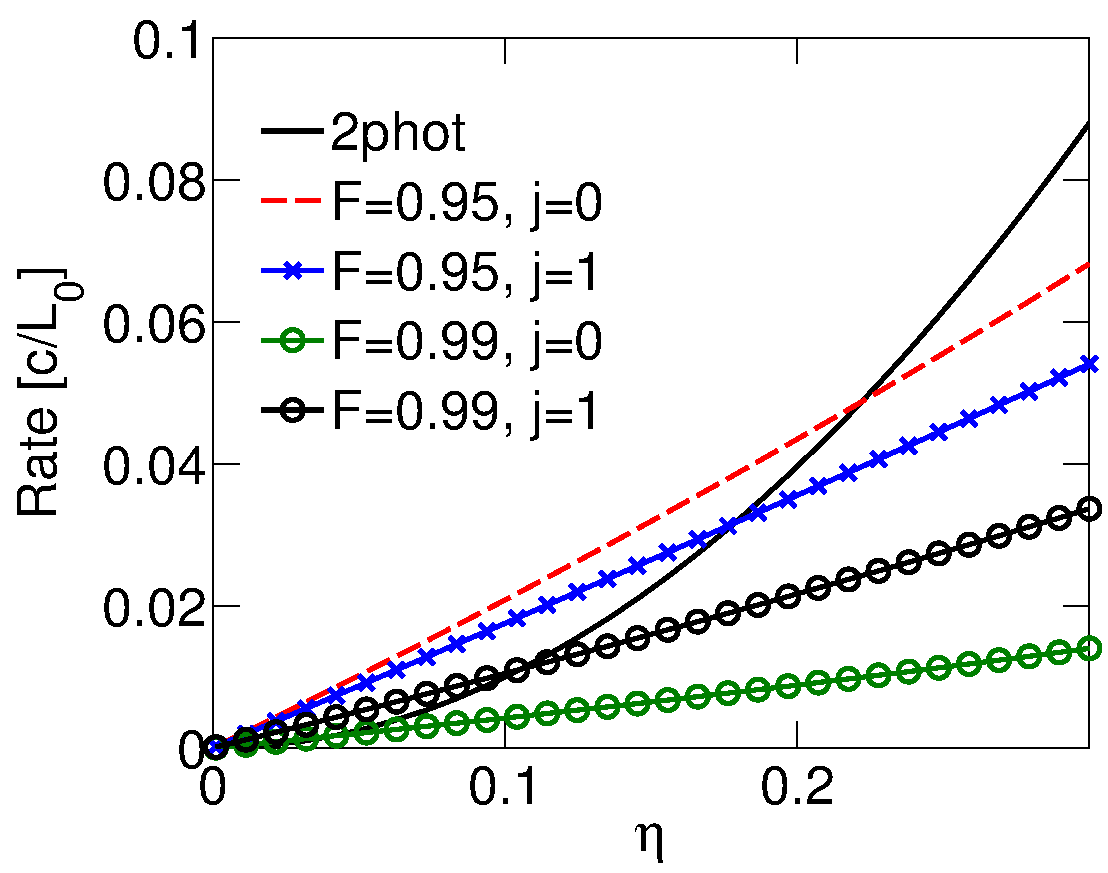
\includegraphics[width=0.6\textwidth]{./figs_Borregaard_PRA2015/figureX3}
\caption[Purification]{Rate of entanglement generation for the two-photon scheme
and the single-photon scheme with target fidelity $F\geq0.95$ and $F\geq0.99$
both without purification ($j=0$) and with one round of purification ($j=1$).
The rate is shown as a function of the total detection efficiency $\eta$. We
have neglected dark counts and assumed that the CNOT gate is deterministic and
have perfect fidelity. The rate has been calculated as described in
App.~\ref{app:rate}. Furthermore, we have assumed that each repeater station
contains 4 qubits, which are either used for purification or to increase the
rate of the entanglement generation. }
\label{fig:figureX3}
\end{figure} 

\subsection{CNOT gates} \label{sec:CNOTgate}

In our analysis, both the initial purification and the subsequent entanglement
swapping involves a cavity-based CNOT gate. Besides the heralded CNOT gate used
in the high-fidelity repeater, which we will refer to as \emph{gate 1}, a
deterministic cavity-based gate proposed in Ref.~\cite{Anders2prl} could be
used. Combining the gate scheme of Ref.~\cite{Anders2prl} with the local
entanglement generation scheme of Ref.~\cite{Anders1prl} results in a
deterministic CNOT gate with an error scaling as $1/C$.  We will refer to this
gate as \emph{gate 2}. This gate does not require an auxiliary atom as gate 1
but rather two auxiliary levels in the qubit atoms as shown in
\reffig{fig:figure4}(a).
\begin{figure}
\centering
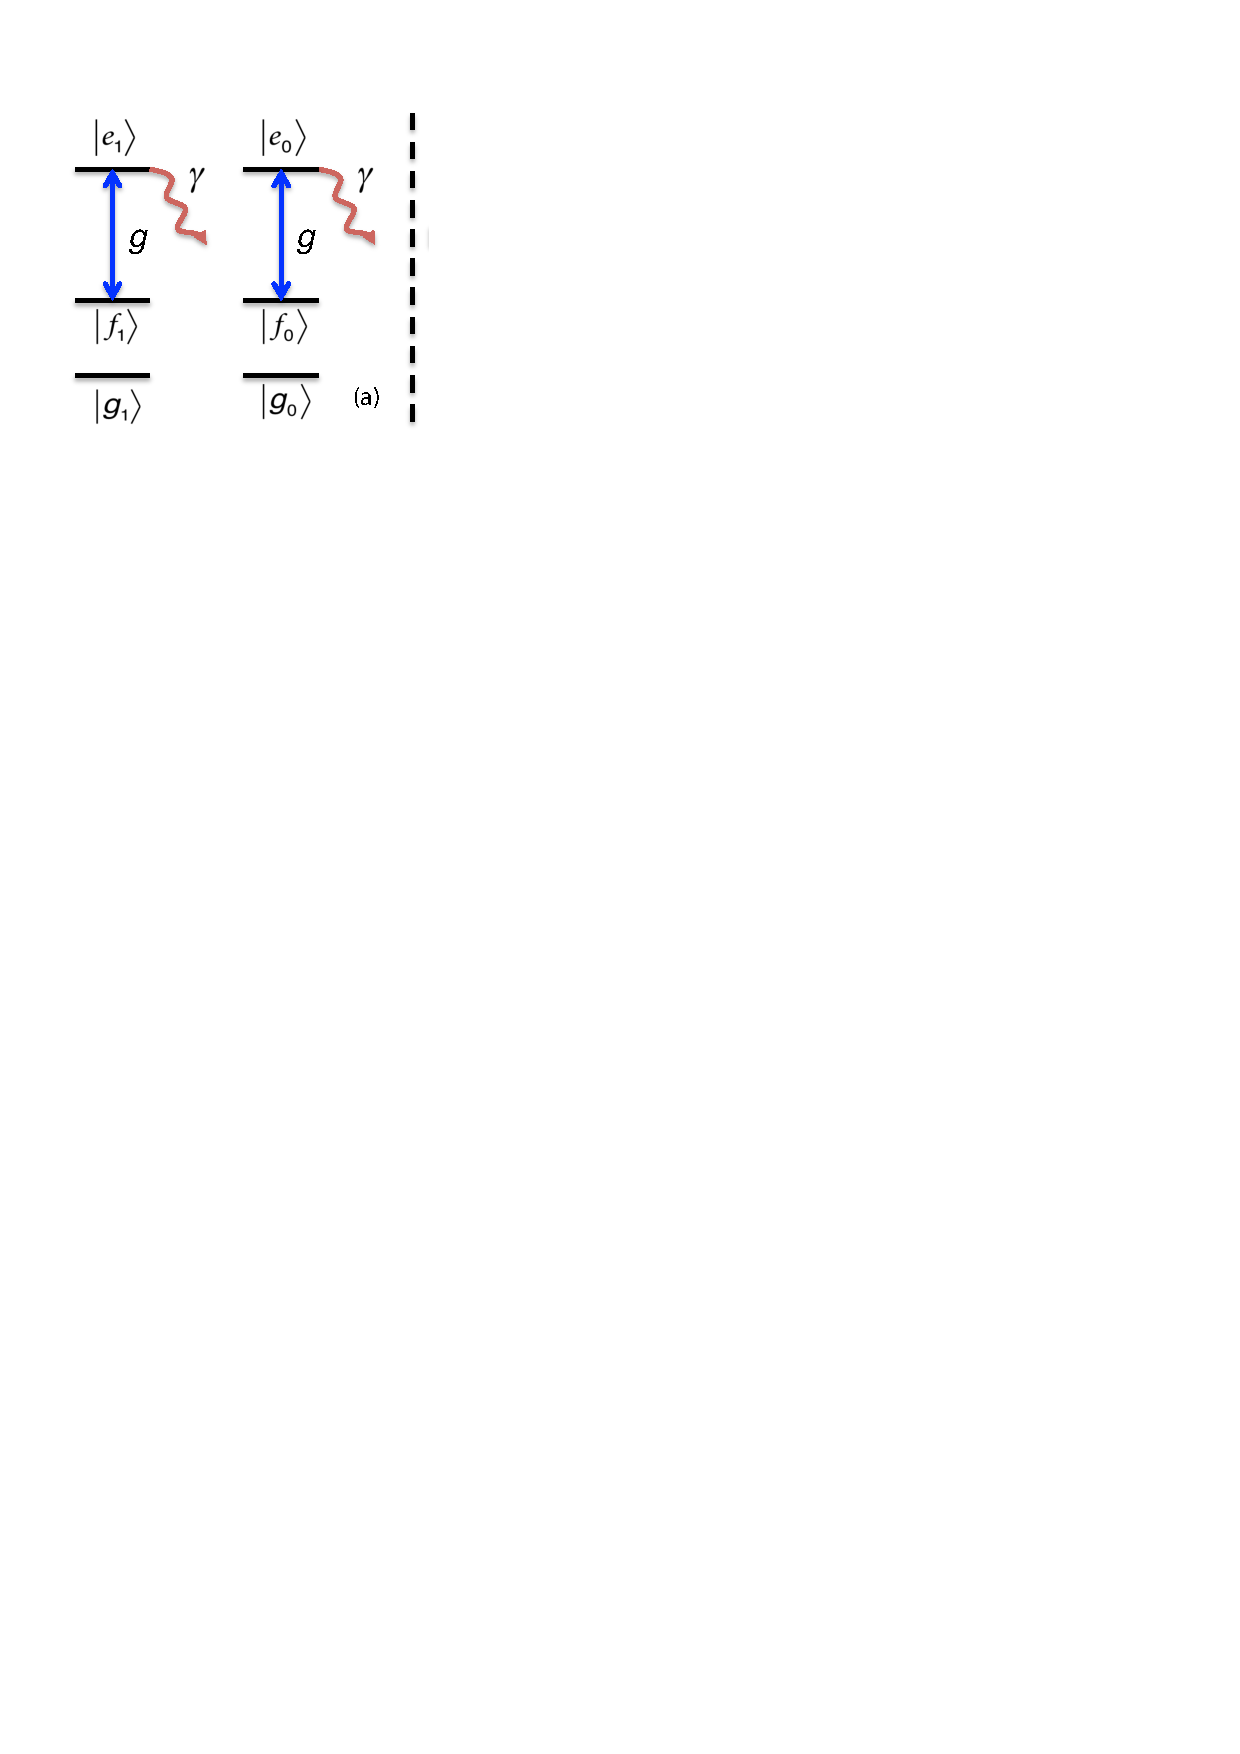
\includegraphics[width=0.4\textwidth]{./figs_Borregaard_PRA2015/figure4a}
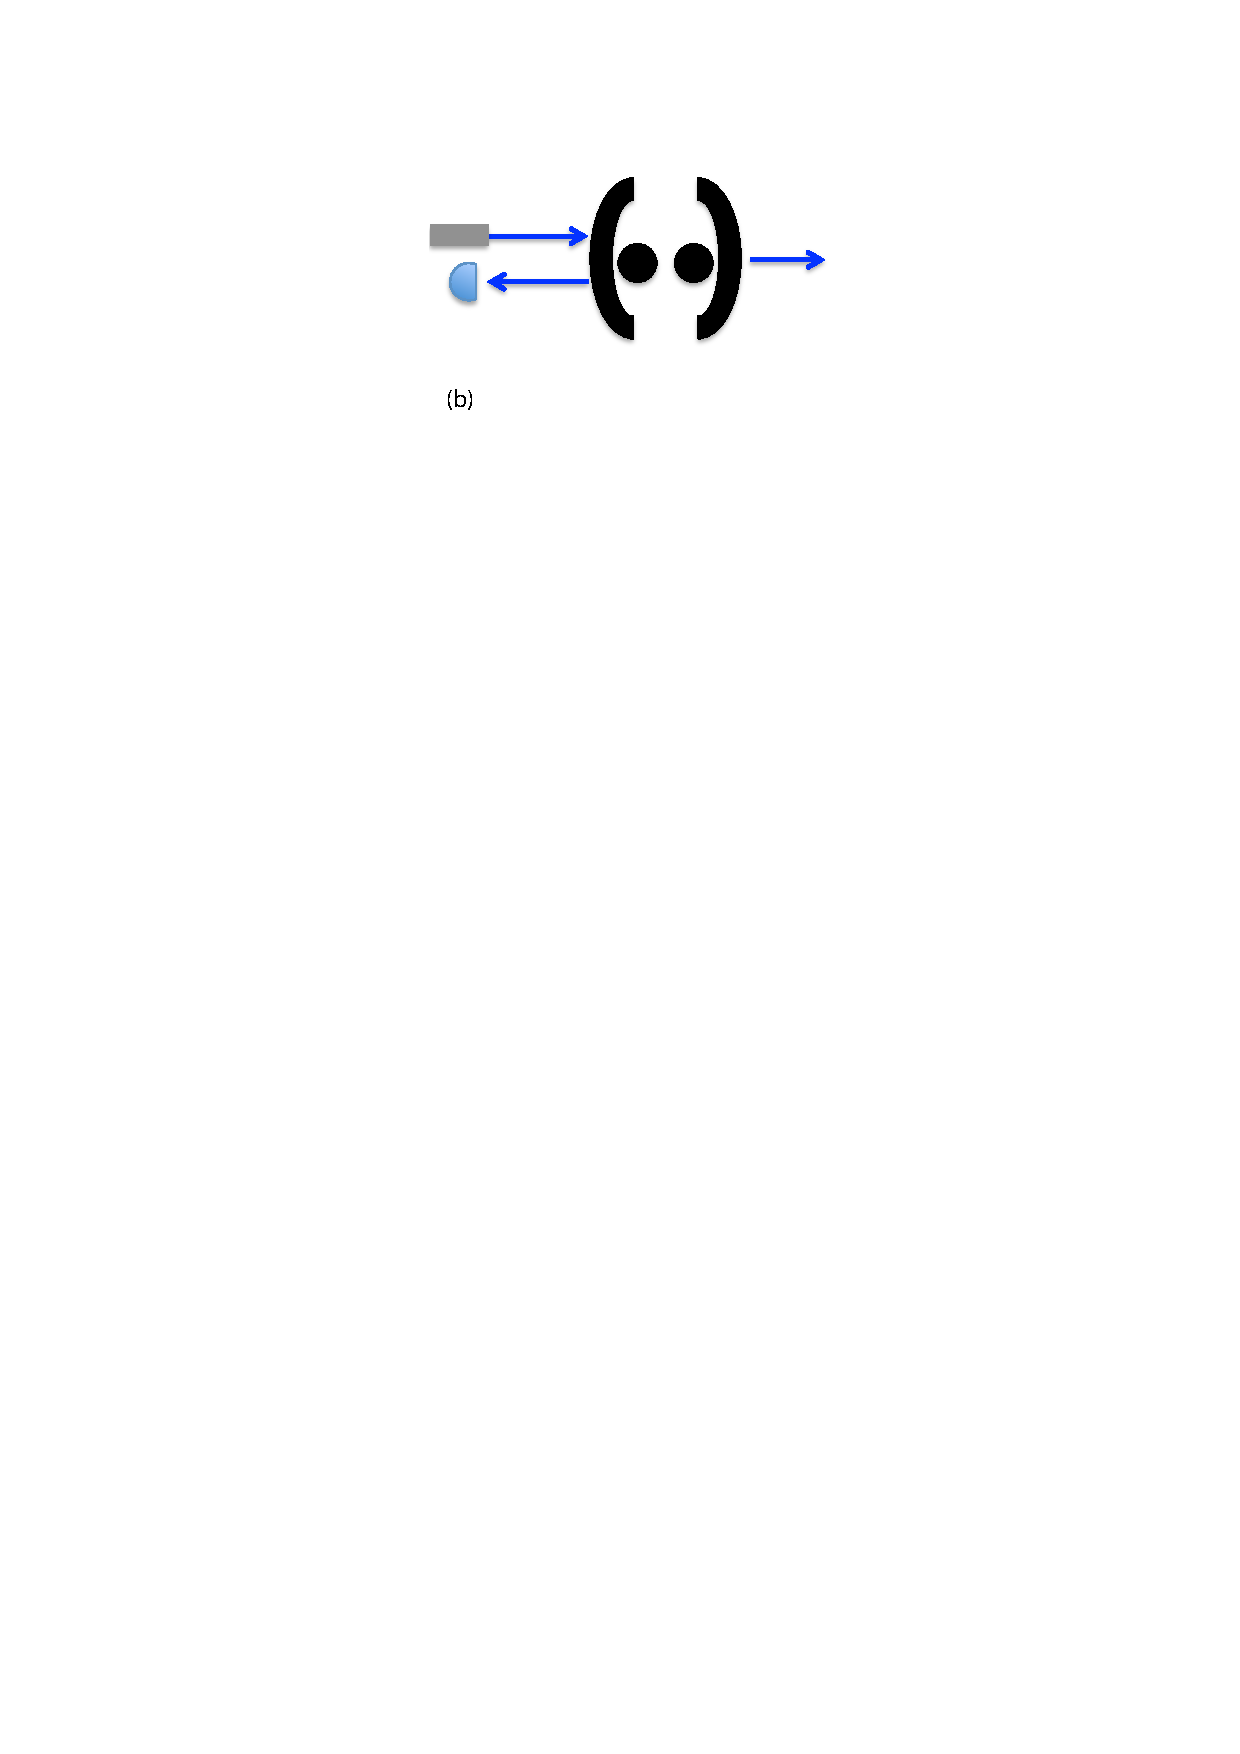
\includegraphics[width=0.4\textwidth]{./figs_Borregaard_PRA2015/figure4b}
\caption[CNOT gate structure]
{Deterministic gate based on reflection and
teleportation based CNOT operation~\cite{Anders1prl,Anders2prl}(a) Level
structure of the qubit atoms. The levels $\ket{r_{0}}$ and $\ket{r_{1}}$ where
$r=g,f$ or $e$ are assumed to be degenerate such that the quantum information is
encoded in the horizontal degrees of freedom. (b) The setup to create
entanglement between the level states $\ket{g},\ket{f}$ of the atoms. Weak
coherent light is sent onto the cavity and any reflected light is measured with
a SPD. }
\label{fig:figure4}
\end{figure}
In this scheme, the quantum information is stored in the horizontal/qubit degree
of freedom (subscripts $0$ and $1$) and the vertical/level degree of freedom
(denoted $g$ and $f$) is used to make an entanglement assisted CNOT gate between
the atoms. Separating the qubit degree of freedom from the level degree of
freedom, the gate works by ideally making the transformation
\begin{equation} \label{eq:transgate1}
\ket{q1}\ket{q2}\otimes\ket{gg}\to
\ket{q1}\ket{q2}\otimes\frac{1}{\sqrt{2}}\left(\ket{gf}+\ket{fg}\right),
\end{equation} 
where $\ket{g},\ket{f}$ denote the vertical states and $\ket{q1}$ ($\ket{q2}$)
is the qubit state of the first (second) qubit, which could be entangled with
atoms at neighboring repeater stations. The entanglement between the levels
$\ket{g}$ and $\ket{f}$ can be used to make a CNOT gate, if the levels of the
atoms can be measured non-destructively, i.e. without revealing any information
about the qubit state as described in Ref.~\cite{Anders2prl}. Both the
transformation shown in Eq.~\eqref{eq:transgate1} and the non-destructive
measurements can be obtained by sending a weak coherent pulse onto a two-sided
cavity and detecting any reflected light (see \reffig{fig:figure4}(b) and
App.~\ref{app:cnot}). If the light is resonant with the empty cavity mode, atoms
in $\ket{f}$ will shift the cavity resonance. Consequently, photons will be
reflected and constitutes a QND measurement of the presence of atoms in
$\ket{f}$. Spontaneous emission from the atoms will limit the fidelity of the
gate to $F\sim1-1.2/(\eta_{\mathrm{d}}C)$, where $\eta_{\mathrm{d}}$ is the
detection efficiency and $C=g^{2}/\kappa\gamma$ is the cooperativity. The gate
time is limited by the time of the single qubit rotations and the coherent
pulses.  We assume that this gives a gate time on the order of 10 $\mu$s.

As a benchmark, we also consider a naive approach where a direct gate between
two qubits is made in a cavity without the use of an auxiliary atom or auxiliary
atomic states. To characterize such a gate, we consider a situation where the
setup of gate 1 is used to make a deterministic gate by simply ignoring the
heralding condition. We will refer to this gate as \emph{gate 3}. For such a
gate, we find that the gate fidelity will scale as $1-F\sim3/\sqrt{C}$ and the
time of the gate will be limited by the time of the single qubit rotations which
we assume to be $\sim10$ $\mu$s.

The characteristics of the three gates we consider are summarized in
\tabref{tab:table2} and illustrated in \reffig{fig:figureX2}.
\begin{table} 
\centering
\begin{tabular}{|c|c|c|c|}
\hline
Gate & Fidelity & Probability & Gate time  \\ \hline
1  & $F=4\cdot10^{-5}$ & $P_{g}\sim1-6/\sqrt{C}$ & $377/(\gamma\sqrt{C})$+10 $\mu$s\\ \hline
2 & $F\sim1-1.2/(\eta_{\mathrm{d}}C)$ & $P_{g}=1$ &10 $\mu$s  \\ \hline
3 & $F\sim1-3.6/\sqrt{C}$ & $P_{g}=1$ &10 $\mu$s \\ \hline
\end{tabular}
\caption
[Characteristics of the three gates]
{Characteristics of the three gates considered for the
cavity-based repeaters. $C$ is the cooperativity of the atom-cavity system and
$\eta_{\mathrm{d}}$ is the single photon detection efficiency in gate 2. The time
of the single qubit rotations is assumed to be 10 $\mu$s. }
\label{tab:table2}
\end{table}
\begin{figure} 
\centering
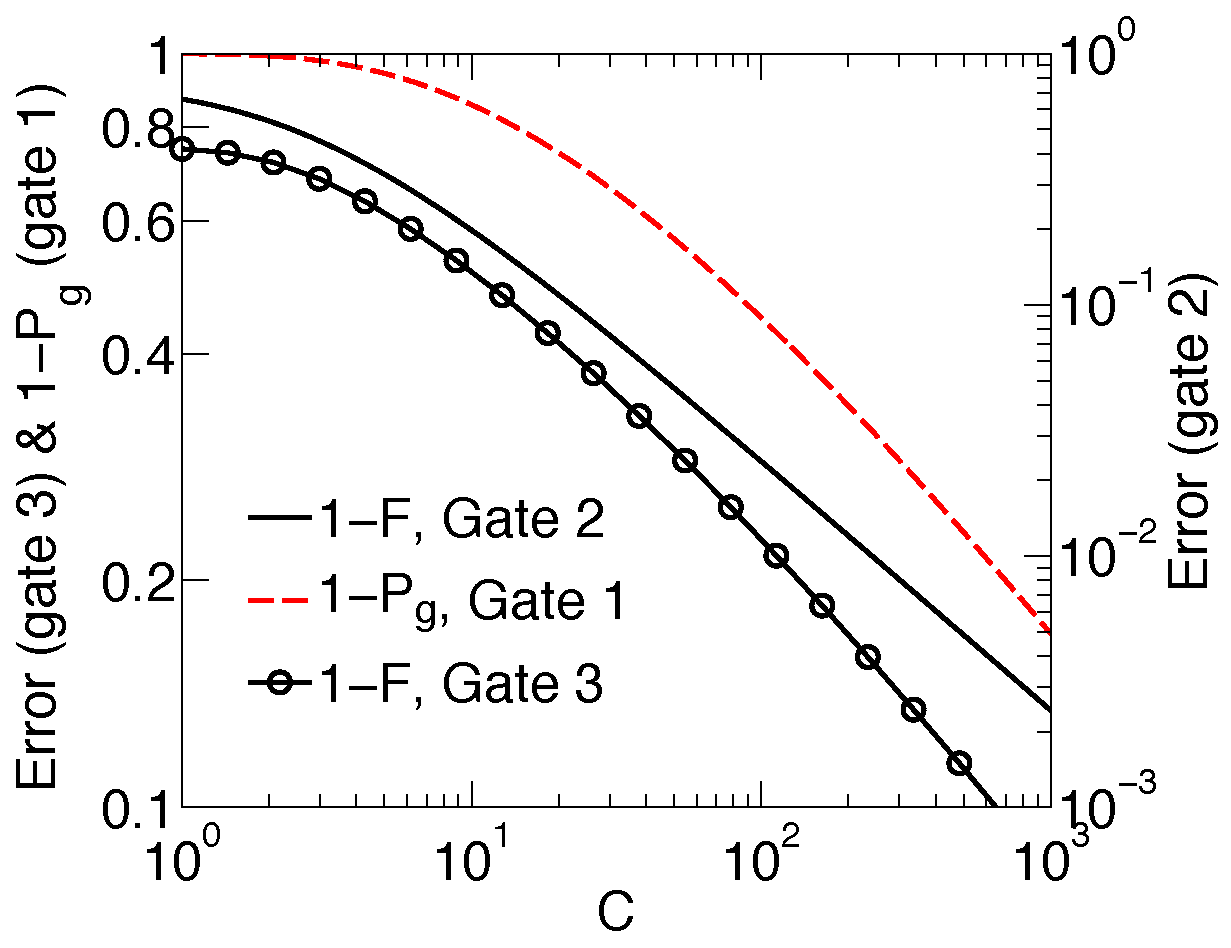
\includegraphics[width=0.6\textwidth]{./figs_Borregaard_PRA2015/figureX2}
\caption[CNOT gates comparison]{Characteristics of the three gates described in
the text. The errors of gate 2 (black/solid line, right axis) and gate 3
(black/circled line, left axis) are shown as a function of the cooperativity.
The error is defined as $1-F$ where $F$ is the fidelity of the gate. We have
assumed $\eta_{d}=0.5$ for the error of gate 2. Gate 1 has conditional fidelity
$\sim1$ but a finite failure probability $1-P_{g}$ which is also shown as a
function of cooperativity (red/dashed line, left axis).}
\label{fig:figureX2}
\end{figure} 
It is clear, that a repeater based on gate 3 will never be advantageous but we
consider it as a reference since the physical requirements for implementing this
gate are less than for gate 1 and 2, which requires either an auxiliary atom or
auxiliary atomic levels.

\section{Numerical optimization} \label{sec:optim}
We have numerical optimized the secret key rate per repeater station for both
the high-fidelity repeater and all other cavity-based repeaters consisting of
the elements considered in Sec.~\ref{sec:other}. The secret key rate is
calculated as described in Sec.~\ref{sec:secret} and App.~\ref{app:rate}. It
depends on experimental parameters such as the efficiency of single photon
detectors, dark count rates. The values of these parameters are assumed
fixed and are thus not part of the optimization.  All the experimental
parameters are summarized in \tabref{tab:parameter} together with the values
assumed in the optimizations. We have assumed fiber transmission losses for
telecom wavelengths, which may require wavelength conversion techniques
\cite{boris}.
{
\ssp
\begin{table}
\centering
\begin{tabular}{| c | c| p{8cm} | }
\hline
Parameter & Value & Description \\ \hline
$\gamma$ & $2\pi \cdot 6$ MHz & Spontaneous emission rate of atoms. This enters in the probability of emitting a photon in the entanglement generation schemes (see Eq.~\eqref{eq:phot1}) and in the gate time of gate 1 and 2. \\ \hline
$\eta_{\mathrm{d}}$ & $50\%$ & Combined efficiency of SPD detectors and outcoupling of light from the cavities. This enters in the total detection efficiency $\eta$ in the entanglement generation schemes since $\eta=\eta_{\mathrm{d}}\eta_{\mathrm{f}}$. It also enters the fidelity of gate 2. \\ \hline 
$L_{att}$ & 22 km  & Attenuation length of the fibers. The total transmission probability over a length $L$ is assumed to be $\eta_{\mathrm{f}}=e^{-L/L_{att}}$. The value assumed corresponds to telecom wavelengths.  \\ \hline
$\tau_{\mathrm{local}}$ & 10 $\mu$s & Time of local qubit operations  \\ \hline
$r_{dark}$ & 25 Hz & Dark count rate of SPD detectors. We include dark counts in the entanglement generation step but not in the gate operations since the gate operations are assumed to be fast.  \\ \hline
$c$ & $2\cdot 10^{5}$ km/s & Reduced speed of light in the transmission fibers \cite{sangouard3}. \\ \hline
\end{tabular}
\caption[Parameters in the numerical optimization]{Experimental parameters which
influence the rate and fidelity of the repeaters. The second column gives the
values used in all optimizations.}
\label{tab:parameter}
\end{table}
}
The free parameters in the optimizations are the number of swap levels, the
number of purifications with/without the modification of Ref.~\cite{nickerson}
and whether a parallel or sequential repeater protocol is used. In the
optimizations, we calculate the secret key rate on a grid of all these
parameters and pick the combination giving the highest rate.
\reffig{fig:figureX6} shows a specific example where the combination of the
single-photon scheme with gate 2 is investigated for a parallel repeater and a
cooperativity of 100.
\begin{figure} 
\centering
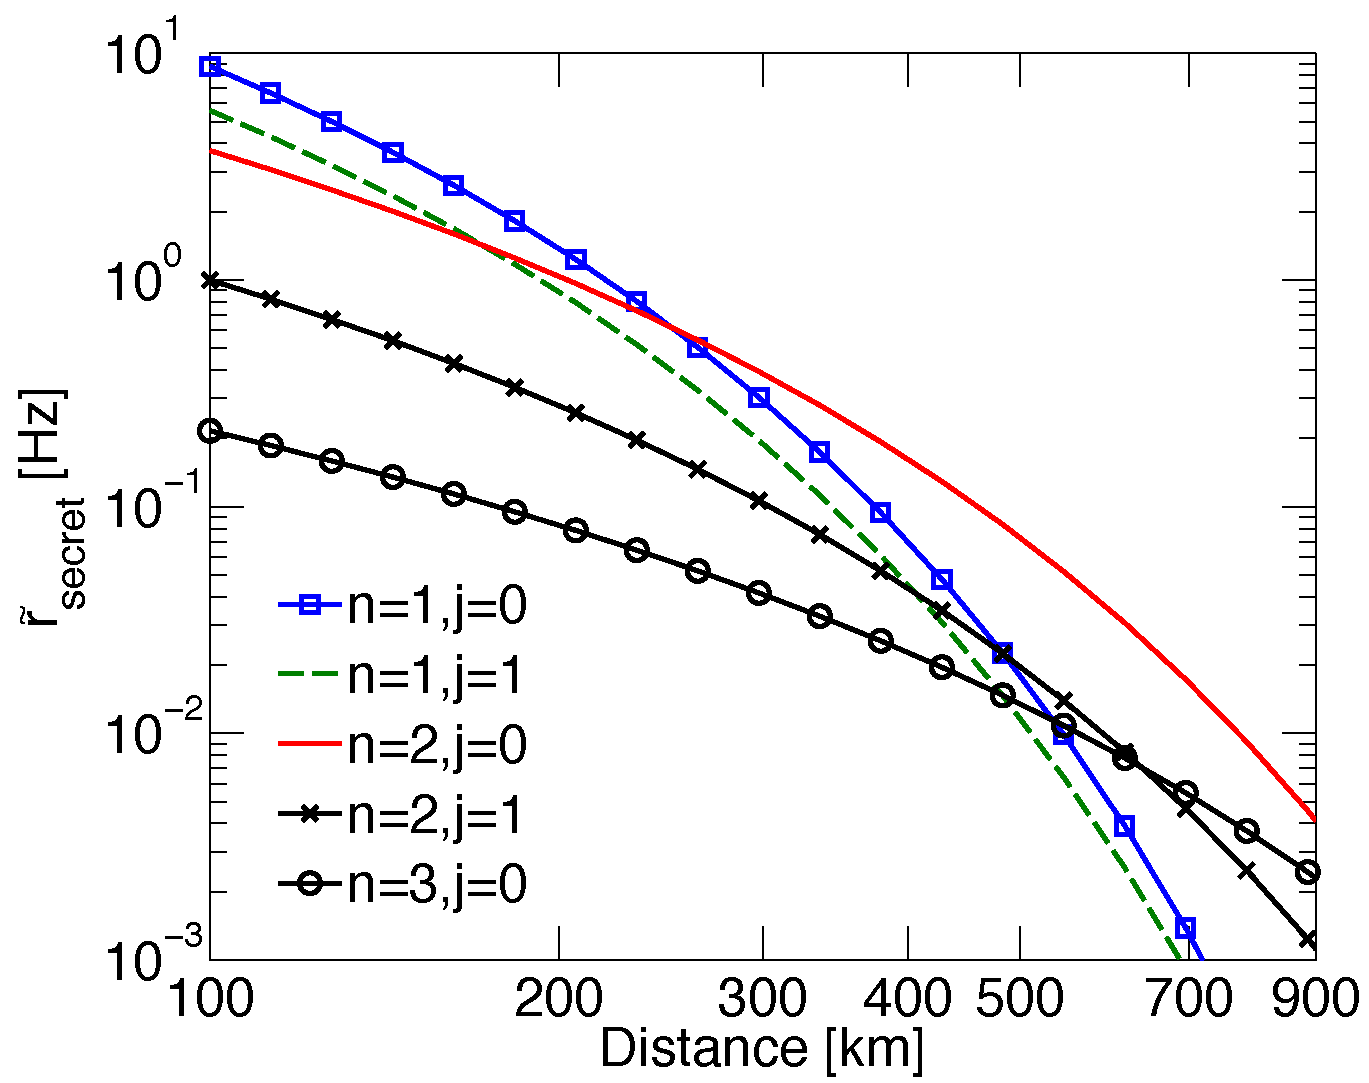
\includegraphics[width=0.65\textwidth]{./figs_Borregaard_PRA2015/figureX6}
\caption[Example of repeater architecture]{Normalized secret key rate per
station($\tilde{r}_{\mathrm{secret}}$) as a function of the distribution distance
(Distance) for a parallel repeater based on the single photon generation scheme
and gate 2. The cooperativity was assumed to be 100 and we assumed 4 qubits per
repeater station. The optimal number of swap levels ($n$) and purification
rounds ($j$) for a given distance can be directly read off from the plot as the
combination giving the highest rate. Note that because the gate fidelity is
limited, curves with $j=2$ and $n=3,j=1$ are not shown since they result in a
much lower secret key rate. The purification schemes was considered to be
without the modification of Ref.~\cite{nickerson}.}
\label{fig:figureX6}
\end{figure} 
The number of swap levels and purifications, giving the highest rate for a
specific distance, can be directly read off from the figure. The same
calculations are then done for a sequential repeater protocol and compared to
the parallel repeater protocol with/without the modified purification in order
to find the highest rate for this specific combination of entanglement
generation scheme and CNOT gate. This is done for all combinations of
entanglement generation schemes and CNOT gates. The optimal evolution time, $T$,
and excitation probability, $\epsilon$, in the entanglement generation schemes
are found for each grid point using a built-in numerical optimization in the
program MATLAB.
The key parameter, determining the performance of the CNOT gates, is the
cooperativity (see \tabref{tab:table2}). We therefore optimize for
cooperativities $C\in[10;1000]$ and distances between 100 km and 1000 km.
Finally, the optimizations are performed for both 2 qubits per repeater station
and 4 qubits per repeater station. Note that the auxiliary atom used in gate 1
is not counted as a qubit and schemes based on this gate thus in principle
contain an additional atom per repeater station.

We model the effect of the non-perfect gates, as depolarizing channels such that
the output of a gate operation described by a unitary $U_{\mathcal{S}}$ working
on a set $\mathcal{S}$ of two qubits is
\begin{equation} \label{eq:gateerror}
\tilde{\rho}=F'U_{\mathcal{S}}\rho
U^{\dagger}_{\mathcal{S}}+\frac{1-F'}{4}\left(\mathrm{Tr}
\left\{\rho\right\}_{\mathcal{S}}\otimes\mathds{1}_{S}\right),
\end{equation}
where $F=F'+(1-F')/4$ is the fidelity of the gate, $\mathds{1}_{\mathcal{S}}$ is
the identity matrix of the set, $\mathrm{Tr}\{\ldots\}_{\mathcal{S}}$ is the
trace over the set and $\rho$ is the initial density matrix describing the system
before the gate operation. We use Eq.~\eqref{eq:gateerror} to propagate the
density matrix from the entanglement generation (see
App.~\ref{single}-\ref{two}) through the steps of initial purification and
entanglement swapping and calculate the average fidelity of the distributed
pairs. To calculate the secret key fraction, we treat the distributed pairs as
Werner states as described in section \ref{sec:secret}.
\begin{figure} [H]
\centering
% 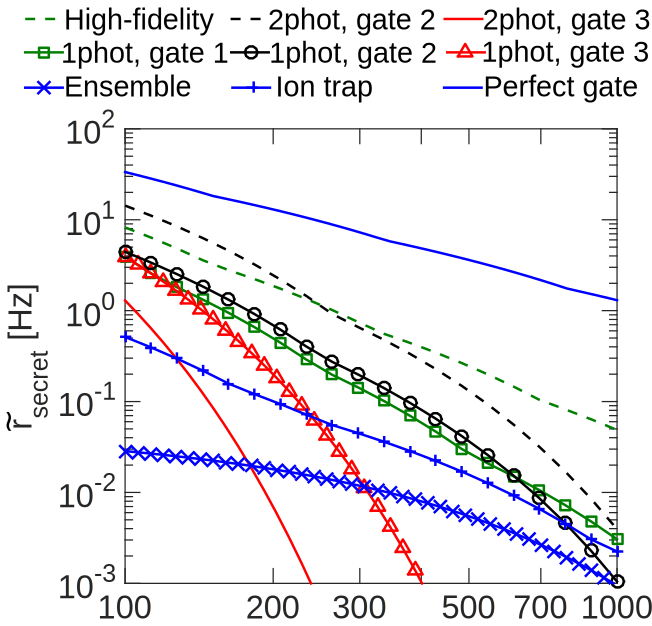
\includegraphics[width=0.48\textwidth]{./figs_Borregaard_PRA2015/figureX7a}
% 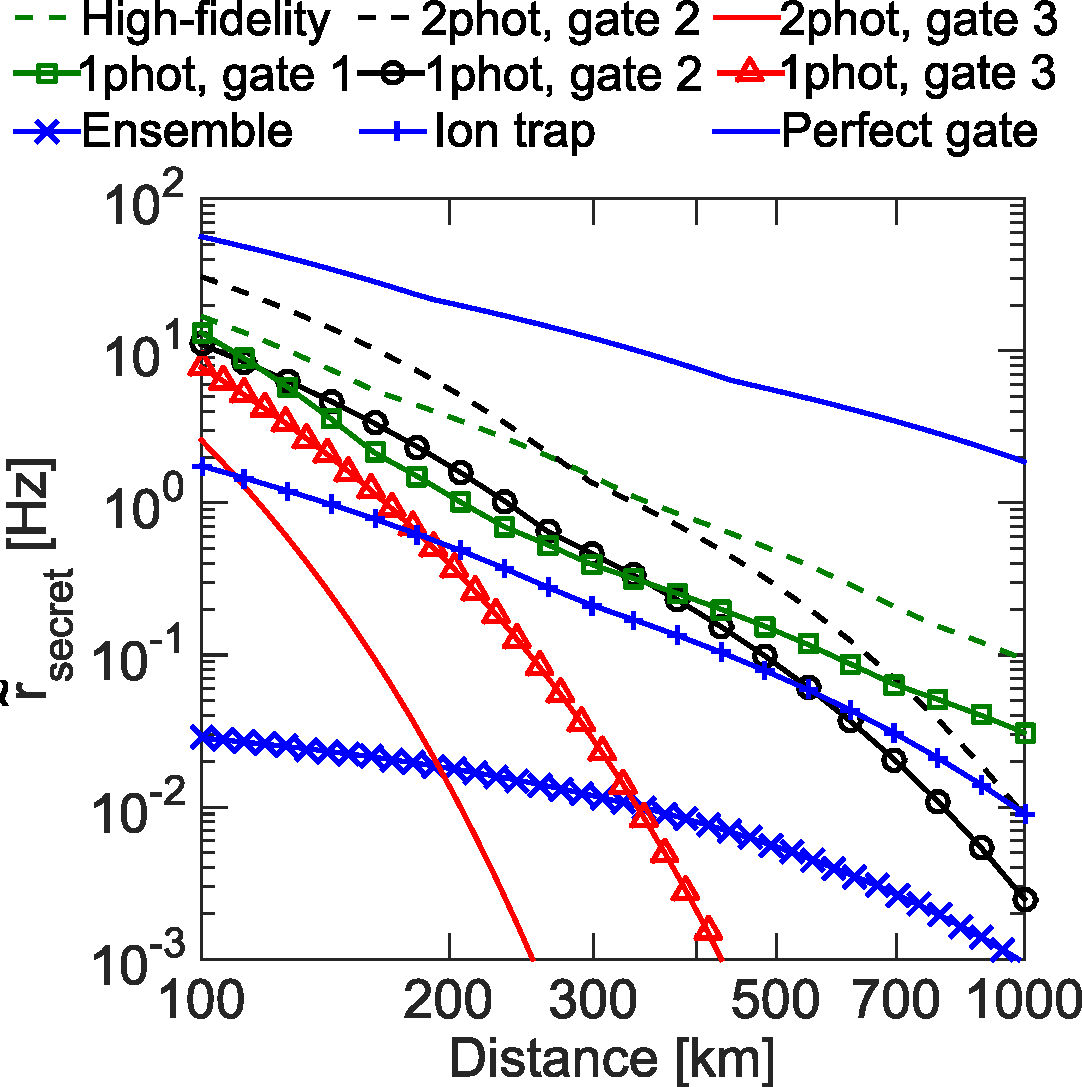
\includegraphics[width=0.48\textwidth]{./figs_Borregaard_PRA2015/figureX7b}
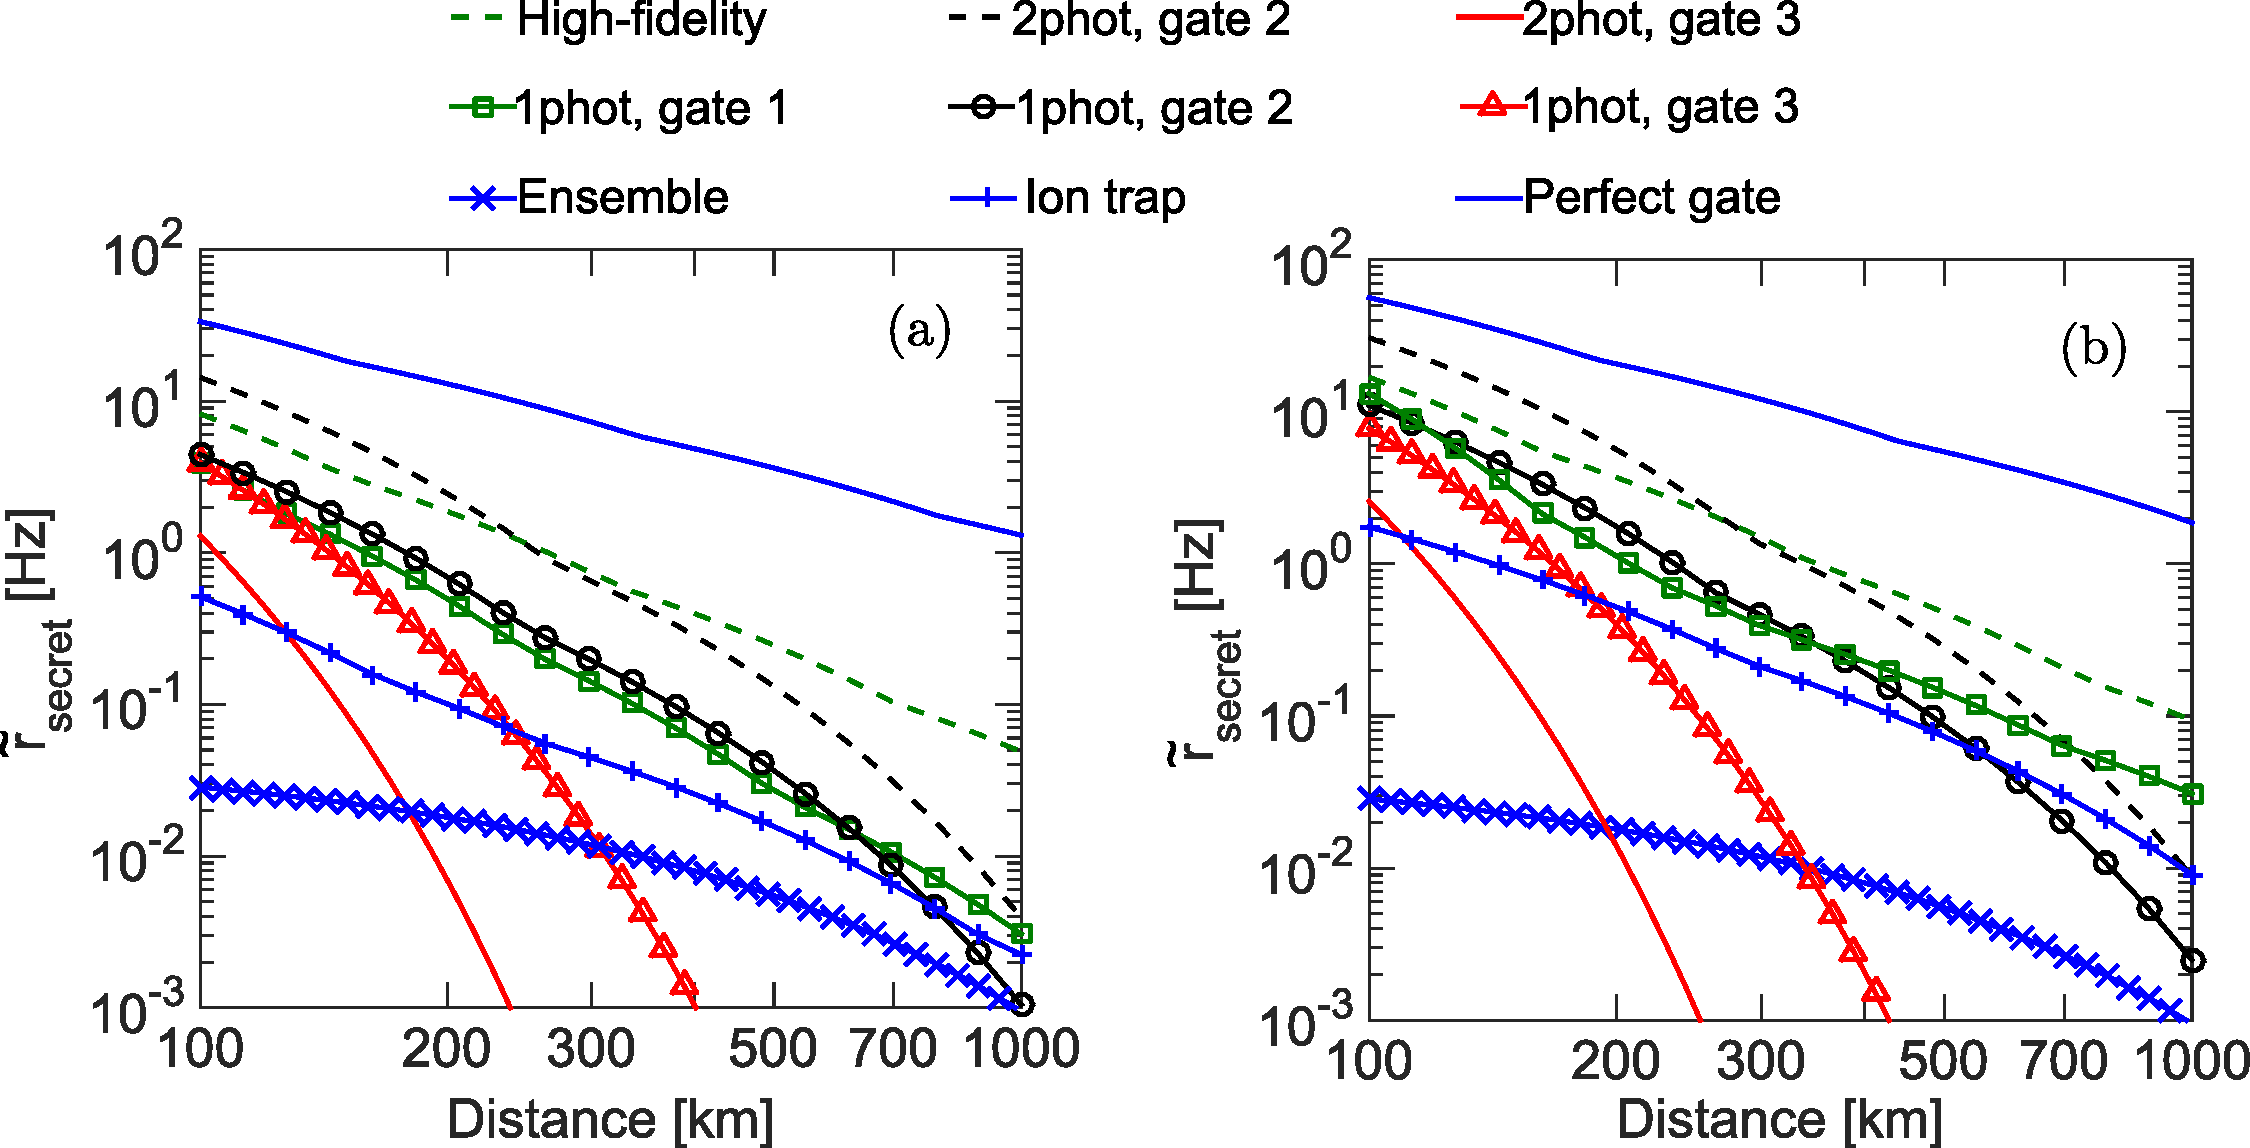
\includegraphics[width=1\textwidth]{./figs_Borregaard_PRA2015/figureX7}
\caption[Optimal secret key rate I]    
{Normalized secret key rate per station
($\tilde{r}_{\mathrm{secret}}$) as a function of the distribution distance
(Distance) for the high-fidelity repeater and other cavity-based repeaters
assuming a cooperativity of $C=$100. (a) is for 2 qubits per repeater station
while (b) is for 4 qubits per repeater station. The other cavity-based repeaters
are labelled as, e.g., ´``1phot, gate 2'', which indicates that it is a
repeater based on the single-photon detection scheme and gate 2. The rate of an
ensemble-based repeater (´``Ensemble'') is also shown~\cite{sangouard1}. For
simplicity, we have assumed a fixed number of four swap levels in the
ensemble-based repeater even though a smaller number of swap levels might
increase the rate for small distances ($\lesssim400$ km). Finally, we have
plotted the rate of an ion trap repeater scheme (´``Ion trap'') with a
collection efficiency of 10\% and gate fidelity of 99.3\% and the ultimate rate
obtainable with perfect deterministic gates and perfect entanglement generation
with the two-photon scheme (´``Perfect gate'') for comparison. For the ion trap
repeater we have plotted the highest rate obtainable with either the one-photon
or two-photon scheme.}
\label{fig:figureX7}
\end{figure} 
\begin{figure} [H]
\centering
% 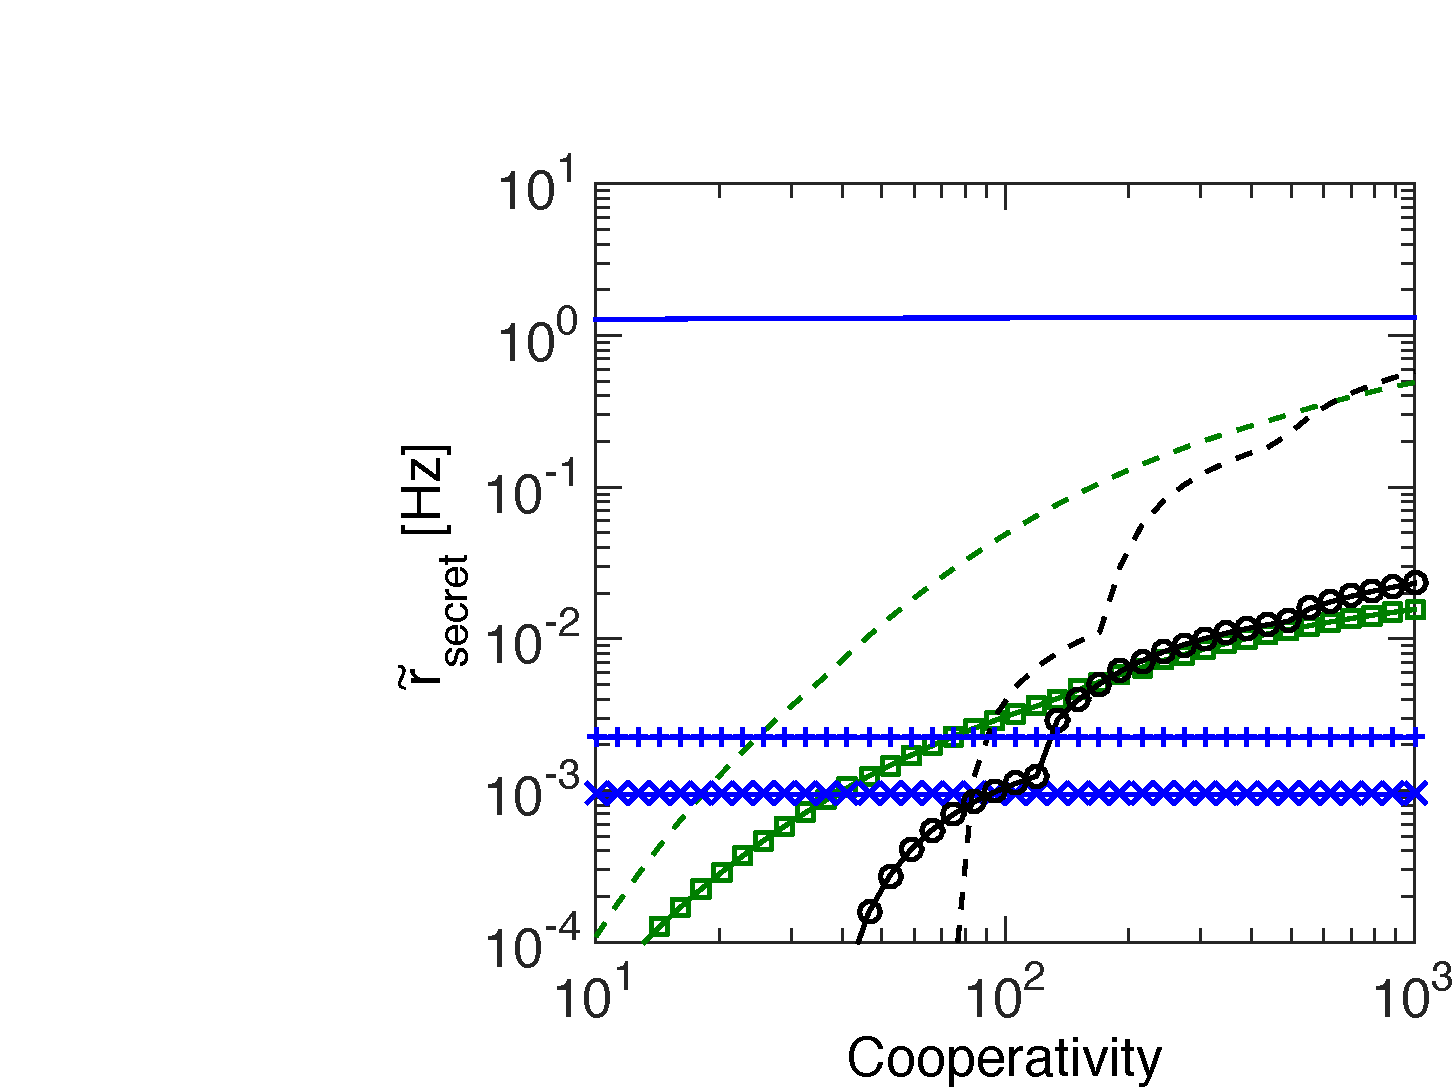
\includegraphics[width=0.48\textwidth]{./figs_Borregaard_PRA2015/figureX8a}
% 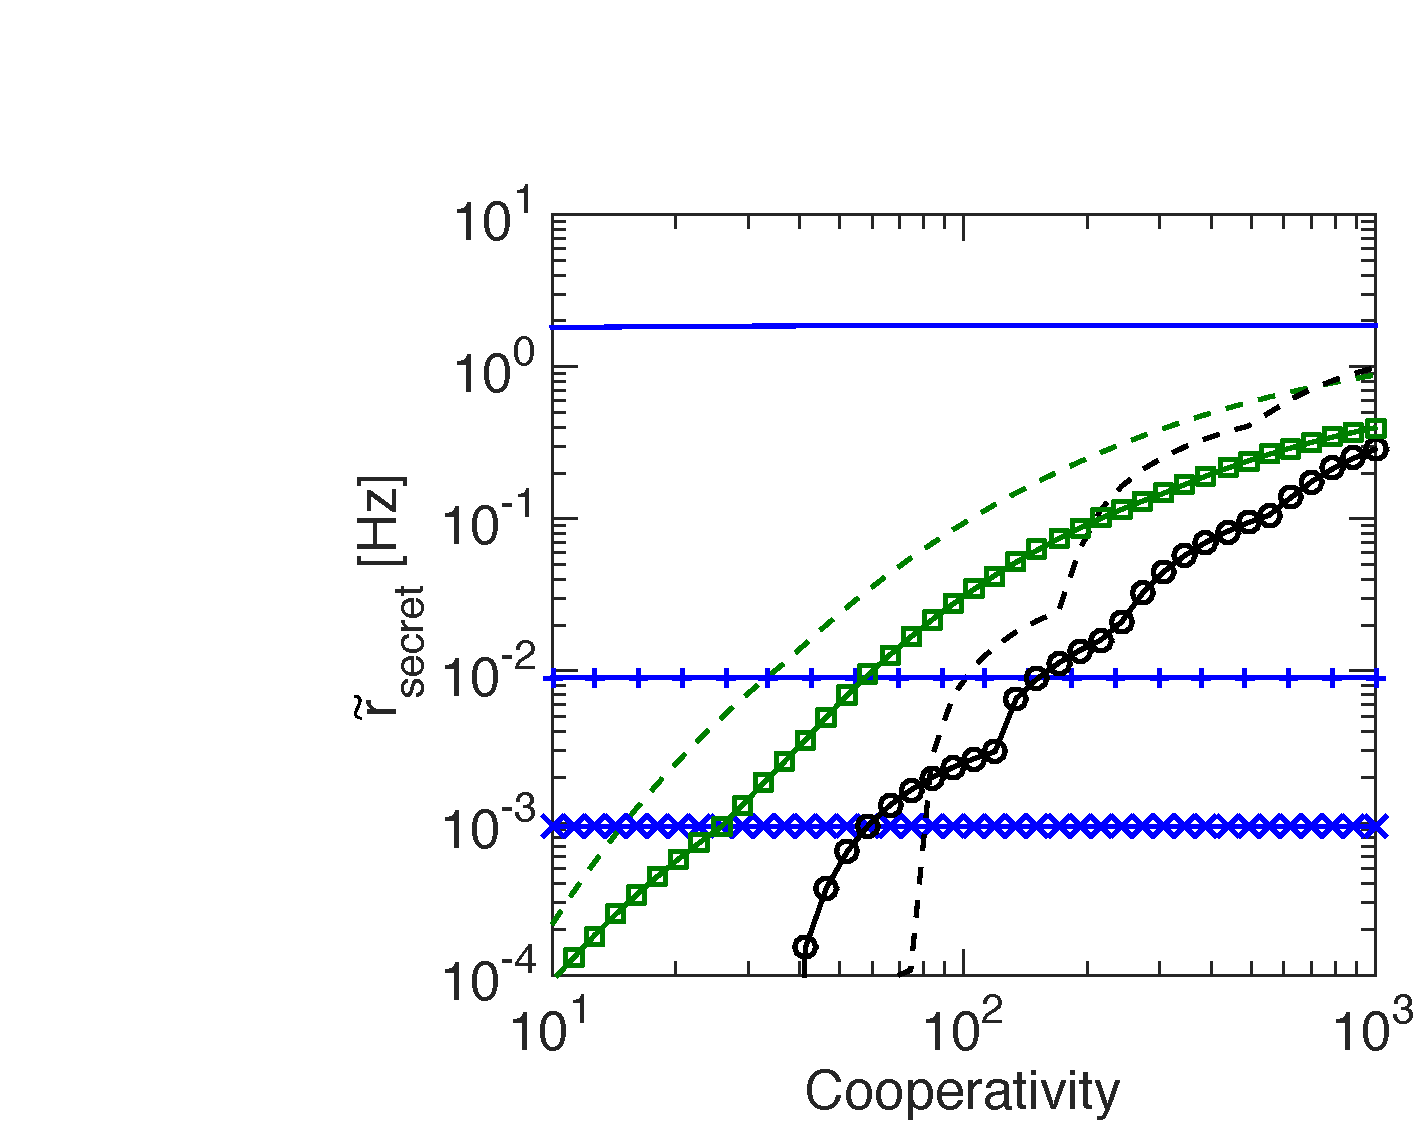
\includegraphics[width=0.48\textwidth]{./figs_Borregaard_PRA2015/figureX8b}
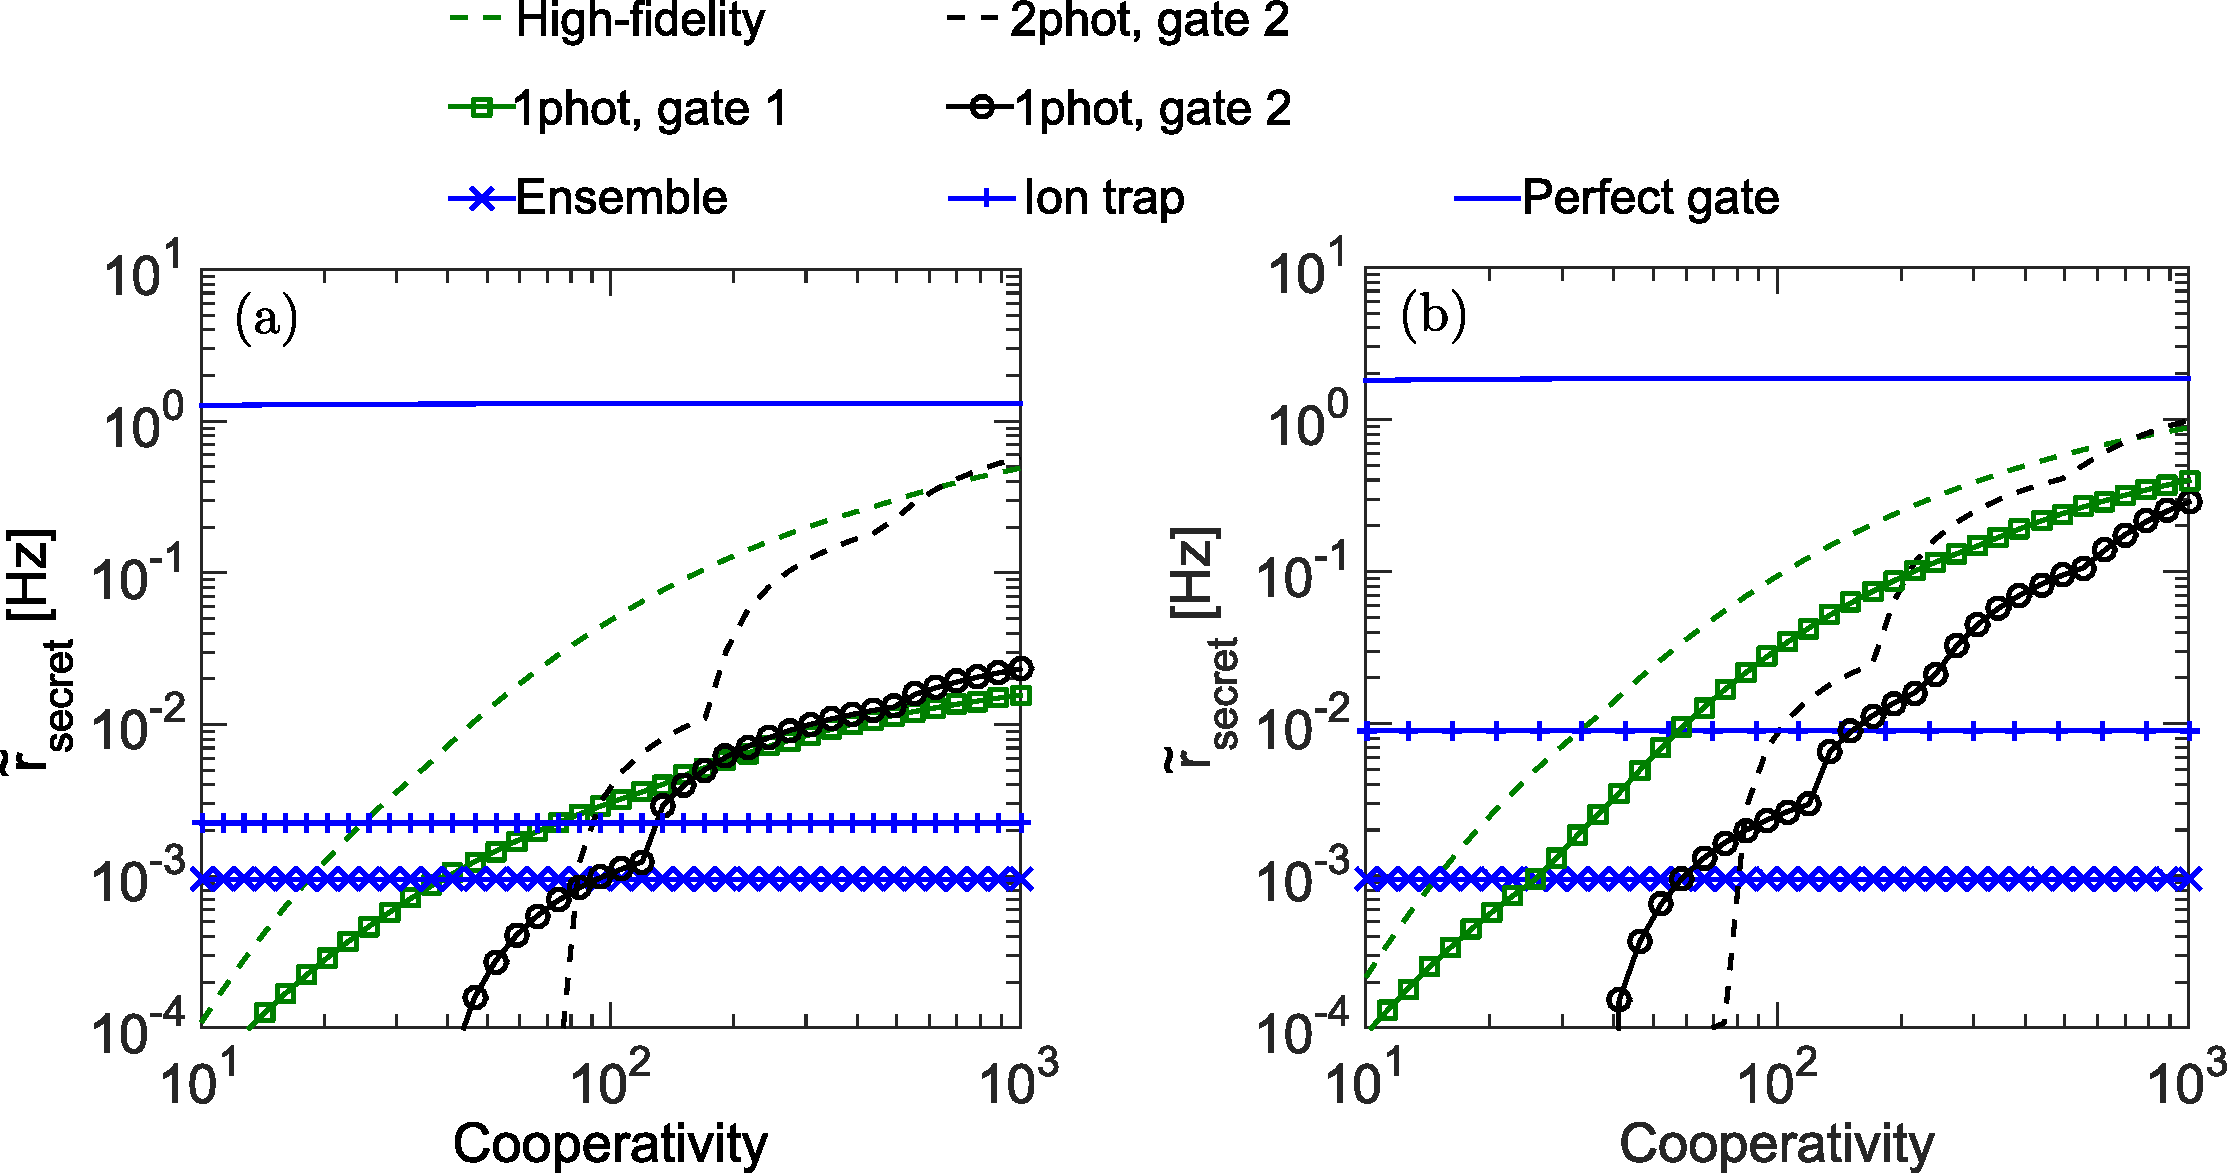
\includegraphics[width=1\textwidth]{./figs_Borregaard_PRA2015/figureX8.pdf} 
\caption[Optimal secret key rate II]{Normalized secret key rate per station
($\tilde{r}_{\mathrm{secret}}$) as a function of the cooperativity ($C$) for the
high-fidelity repeater and other repeaters assuming a distribution distance of
1000 km. (a) is for 2 qubits per repeater station while (b) is for 4 qubits per
repeater station.}
\label{fig:figureX8}
\end{figure}

The secret key rates per repeater station of the high-fidelity repeater and the
other cavity-based repeaters are shown in Fig.~\ref{fig:figureX7} for distances
$[100;1000]$ km and a cooperativity of 100 and in Fig.~\ref{fig:figureX8} for a
distance of 1000 km and cooperativities in the interval $[10;1000]$. As shown in
\reffig{fig:figureX7}, the repeaters based on gate 3 are simply not able to
distribute entanglement over large distances for realistic cooperativities. As a
consequence, repeaters based on gate 3 do not appear on Fig.~\ref{fig:figureX8}
since their secret key rate is simply too low.

In general, the high-fidelity repeater (2-photon, gate 1) achieves the highest
secret key rate for a broad range of cooperativities and long distances $\gtrsim
300$ km. This reflects both that this protocol allows for a higher number of
swap levels and that the secret key rate favors the distribution of
high-fidelity pairs since these gives the highest secret fraction (see
\reffig{fig:figure5}). It is also apparent from Fig.~\ref{fig:figureX8} that
while repeaters based on gate 2 need cooperativities above 100 for a distance of
1000 km, repeaters based on gate 1 are able to function with much lower
cooperativities around $30-40$. This is because the heralded gate has nearly
unit fidelity, independent of the cooperativity. For high cooperativities or
low distances, a repeater based on the two-photon detection scheme and gate 2
can give a slightly higher secret key rate than the high-fidelity repeater. This
improvement is, however, less than a factor of 2 in the secret key rate. The
steps in the rates of the schemes based on gate 2 in Fig.~\ref{fig:figureX8}
originate from the fact that as the cooperativity increases, the fidelity of
gate 2 increases and at some point the fidelity is high enough to allow for
another swap level, which makes the rate increase abruptly.
From the optimizations, we find that the sequential repeater architecture
achieves slightly higher rates (less than a factor 2) than the parallel repeater
architecture for 4 qubits per repeater station, while the opposite is the case
for 2 qubits per repeater station.

In general, repeaters based on the two-photon detection schemes outperform
repeaters based on the single-photon detection scheme except for repeaters based
on gate 3. This reflects that repeaters based on gate 3 cannot perform many swap
levels since the fidelity simply decreases too rapidly with the number of swap
levels. The result of the optimization was that no swap levels were actually
preferred for repeaters based on gate 3 for $C\leq1000$.  As a result, the
elementary links in these repeaters are long and fiber losses therefore
significantly decrease the total detection probability $\eta$ in the
entanglement generation schemes. In the limit of very low $\eta$, the one-photon
scheme is advantageous since the success probability only depends linearly on
$\eta$. For the optimizations, we have assumed that the combined efficiency of
the SPD detectors and outcoupling of light from the cavities is $\eta_{d}=$50\%.
If this efficiency is smaller, repeaters based on single-photon detection may be
desirable. We also find that the purification protocol, in general, performs
better with than without the modification of Ref.~\cite{nickerson}. The
improvement is, however, limited to a factor of $\lesssim2$ for the parameters
considered in Figs.~\ref{fig:figureX7}-\ref{fig:figureX8}.

It is important to stress that the rates plotted in
Figs.~\ref{fig:figureX7}-\ref{fig:figureX8} are the secret key rates divided by
the total number of repeater stations. The actual distribution rate can thus be
obtained by multiplying with the number of repeater stations. For the
high-fidelity repeater, we find a secret key rate of $\sim$16 Hz over 1000 km
for 33 repeater stations and a cooperativity of 1000 assuming 2 qubits per
repeater station.  For a more modest cooperativity of 100, a secret key rate of
$\sim$1.5 Hz over 1000 km can be obtained.

We can compare the rate found here to the rate obtainable with repeaters based
on atomic ensembles. In Ref.~\cite{sangouard1} an efficient repeater based on
atomic ensembles is described, which achieves one of the highest distribution
rates for repeaters based on atomic ensembles~\cite{sangouard3}. The fidelity of
the distributed pair and the distribution rate are derived in
Ref.~\cite{sangouard1} for a repeater with four swap levels corresponding to 17
repeater stations.  Based on this, we have calculated the secret key rate
assuming an optimistic, basic repetition rate of the ensembles of 100 MHz and
memory and SPD efficiencies of 90\%. The rate of the ensemble-based repeater is
also shown in Figs.~\ref{fig:figureX7}-\ref{fig:figureX8} for similar
assumptions about fiber losses etc. as for the cavity-based repeaters. We have
assumed that the repeater uses four swap levels for all distances even though a
smaller number of swap levels may be desirable for smaller distances
($\lesssim400$ km)~\cite{sangouard1}. For a distance of 1000 km, we find a rate
of $\sim0.03$ Hz for 33 repeater stations. This shows that repeaters based on
individual atoms in cavities may be very promising candidates for realizing
efficient quantum repeaters with rates exceeding those obtainable with atomic
ensembles. The main reason for this is that very efficient entanglement swapping
can be realized in the cavity-based repeaters which greatly enhances the
distribution rates for long distances. On the contrary, repeaters based on
atomic ensembles and linear optics have an upper limit on the swapping
efficiency of 50\%.

For comparison we have also considered a repeater based on ion traps where there
is no cavity to collect the light. Non-local entanglement can still be created
by collecting the emitted light with a lens as demonstrated in
Ref.~\cite{monroe2014} where a collection efficiency of 10\% was reported. The
entanglement swapping can be realized using a gate, which has been demonstrated
experimentally with a fidelity of 99.3\% and a gate time of $50$
$\mu$s~\cite{blatt1}. Note that this fidelity was measured for the generation of
a single state in Ref.~\cite{blatt1} but we will assume it to be the fidelity of
the entanglement swap. The rate of such a ion-trap repeater is shown in
Figs.~\ref{fig:figureX7}-\ref{fig:figureX8} with assumptions about fiber losses
etc. summarized in Tab.~\ref{tab:parameter}. We have assumed a collection
efficiency of 10\% and as a result, the one photon scheme with modified
purification performs better than the two-photon scheme for 4 qubits per
repeater station. However for two qubits, where purification is not possible,
the two-photon scheme is in general advantageous except for small distances ($<$
200 km). We have assumed a gate fidelity of 99.3\% and have plotted the highest
rate obtainable with either the one-photon or two-photon scheme.

It is seen that the high-fidelity repeater outperforms the ion-trap repeater for
$C\gtrsim30$, which is mainly due to the low collection efficiency in the
entanglement generation. The ultimate rate, obtainable with a repeater with
perfect deterministic entanglement swapping and entanglement generation based on
the two-photon detection scheme with a collection efficiency set by $4C/(1+4C)$,
is also shown in Figs.~\ref{fig:figureX7}-\ref{fig:figureX8}. A similar repeater was
considered in Ref.~\cite{sangouard2} to demonstrate the feasibility of repeaters
based on trapped ions. For $C=1000$, the high-fidelity repeater achieves only a
factor of $\sim2$ slower rate than this ultimate limit for a distance of 1000
km.

\section{Conclusion}        

In conclusion, we have performed a detailed analysis of quantum repeaters based
on individual emitters in optical cavities. We have found that a high-fidelity
repeater based on the heralded gate described in Ref.~\cite{Borregaard2015a} combined
with a two-photon detection scheme is the best option over a large parameter
regime and enables high secret key rates over large distances even for limited
cooperativities $<100$. Compared with a number of other cavity based repeaters
it achieves rates that are up to two orders of magnitude faster for long
distances (1000 km) and cooperativities $<100$. For small distances or higher
cooperativities, a repeater based on the deterministic CNOT gate described in
Ref.~\cite{Anders2prl} combined with a two-photon detection scheme can achieve
rates which are slightly higher than the high-fidelity repeater but the
improvement is less than a factor of 2.

We have also compared the high-fidelity repeater to the repeater in
Ref.~\cite{sangouard1}, which is based on atomic ensembles. For a distance of
1000 km and $C\gtrsim20$ the high-fidelity repeater begins to outperform the
ensemble-based repeater and an improvement of more than two orders of magnitude
in the secret key rate is possible for $C\gtrsim100$. The main reason for the
advantage of the high-fidelity repeater is that entanglement can be swapped very
efficiently using the heralded CNOT gate described in Ref.~\cite{Borregaard2015a}.
Consequently, the number of swap levels in the repeater can be increased without
the need of intermediate purification, which greatly enhances the rate for large
distances. A similar advantage could in principle be achieved by resorting to a
trapped ion system, where efficient gates can be implemented. For current
systems, the collection efficiencies are, however, so low that a trapped ion
system could be outperformed by a cavity system with a limited finesse of
$C\gtrsim 30$. If the collection efficiency could be overcome, e.g. by placing
the ions in a cavity with a high cooperativity, the rate can be substantially
improved, but with $C>1000$ the high fidelity repeater investigated here is
within a factor of two of this ideal repeater. It should, however, be noted that
we have compared schemes with strong physical differences in our analysis. The
high-fidelity repeater requires an extra auxiliary atom while auxiliary atomic
levels are required to decrease the error of the deterministic cavity-based CNOT
gates. The ensemble-based and ion-trap repeaters are also very different
physical systems compared to the cavity-based repeaters with individual atoms.
The different experimental difficulties in realizing the physical requirements
for the various repeater schemes should be included in a more advanced
assessment.

Finally, we note that while we have investigated a number of different possible
repeater protocols there may be even more advantageous procedures. Hence the
results that we have derived here should be seen as lower limits to the
achievable communication rates. A particular interesting  possibility could be
to investigate proposals along the lines of Ref.~\cite{cirac1,cirac2}, which
also rely on heralding measurements to detect errors during entanglement
generation and two qubit operations.  Possibly some of the ideas from these
schemes could be used to improve the communication beyond what we have found
here.
  
\chapter{Heisenberg-Limited Atom Clocks Based on Entangled Qubits}
\label{ch:Kessler2014}
% From \cite{Kessler2014}
%%%%%%%%%%%%%%%%%%%%%%%%%%%%%%%%%%%%%%%%%%%%%%%%

%%%%%%%%%%%%%%%%%%%%%%%%%%%%%%%%%%%%%%%%%%%%%%%%%%%%%%%%%%%%%%%%%%%%%%%%%%%%%%%%%%5
%%%%%%%%%%%%%%%%%%%%%%%%%%%%%%%%%%%%%%%%%%%%%%%%%%%%%%%%%%%%%%%%%%%%%%%%%%%%%%%%%%5
\section{Introduction}
%%%%%%%%%%%%%%%%%%%%%%%%%%%%%%%%%%%%%%%%%%%%%%%%%%%%%%%%%%%%%%%%%%%%%%%%%%%%%%%%%%5
%%%%%%%%%%%%%%%%%%%%%%%%%%%%%%%%%%%%%%%%%%%%%%%%%%%%%%%%%%%%%%%%%%%%%%%%%%%%%%%%%%5
Currently, atomic clocks based on optical transitions achieve the most
precise \cite{Nicholson2012, Bloom2013, Lemke2009} and accurate \cite{Chou2010,
Bloom2013} frequency references.
Additionally, the development of optical frequency combs
\cite{Eckstein1978, Reichert2000, Jones2000, Ye2003} -- establishing a coherent
link between the optical and radio frequencies -- enabled the application
of optical frequency standards to a wide range of scientific and technological
fields including astronomy, molecular spectroscopy and global
positioning systems (GPS).

% The improvement of frequency standards using quantum resources, such as
% entanglement, has attracted wide attention in recent years \cite{Buzek1999,
% Andre2004, Rosenband2012, Rosenband2012_numerical}.

The improvement of frequency standards using quantum resources, such as
entanglement \cite{Buzek1999, Andre2004,LouchetChauvet:2010fs,Rosenband2012_numerical,
Borregaard2013_nearHeisenberg},
%, as well as
%schemes consiting of multi-layered interrogation and feedback
%\cite{Rosenband2013, Borregaard2013} 
has been actively explored in recent years. While clock protocols
based on uncorrelated atoms at best achieve a stability scaling
$\propto1/\sqrt{N}$, where $N$ is the number of atoms -- a
scaling commonly known as the standard quantum limit (SQL) \cite{Caves1980} --
the use of entangled resources, in principle, allows one to surpass this limit.
However, a characterization of the improvement obtainable by using entanglement
 requires a detailed investigation of the decoherence present in the system.
 Previous studies have focused on two kind of noise sources: i) single particle
 decoherence resulting from the interaction of the atoms with the environment
 and ii) frequency fluctuations in the laser used to excite the clock transition
 [in the following also referred to as local oscillator (LO)].
  It is well known that fully entangled states (e.g.,
  Greenberger-Horne-Zeilinger (GHZ) states) allow for improved spectroscopic sensitivity, but in the same way
 that these states benefit from their increased sensitivity in the laser
 interrogation, they are generically prone to various types of noise sources
 canceling any quantum gain. It has therefore been long believed that such
 states fail to increase clock stability regardless of the noise model being used
 \cite{Bollinger1996, Wineland1998, Rosenband2012_numerical,Huelga1997}. On the other hand, it has been shown that
for clocks with local oscillator noise limited stability, the use of
moderately squeezed atomic states can yield a modest improvement over the SQL
\cite{Andre2004,LouchetChauvet:2010fs}.
 A recent study demonstrated further that, in principle, highly squeezed states
could achieve Heisenberg-limited stability (i.e., a $1/N$ scaling
with the available resources representing the ultimate limit allowed by the laws
of quantum mechanics \cite{Giovanetti2011}) using a complex adaptive
measurement scheme \cite{Borregaard2013_nearHeisenberg}.
 At the same time, it has been shown that the single particle
 decoherence-limited regime can be reached for long averaging time at
a logarithmic cost in $N$ by interrogating uncorrelated atomic
ensembles for suitably chosen times \cite{Rosenband2013, Borregaard2013}.

In this Letter, we  introduce a protocol involving groups of sequentially larger
GHZ states to estimate local oscillator deviations from the atomic reference in
a manner reminiscent of the phase estimation algorithm \cite{Nielsen_Chuang}.
Furthermore, we unify previous treatments of decoherence for atomic clocks 
and incorporate previous proposals involving uncorrelated atoms to
effectively narrow the LO linewidth \cite{Rosenband2013, Borregaard2013} and thereby identify
 ultimate limits to the stability of atomic clocks based on entangled atoms. We find that for LO-noise limited clocks, the
proposed quantum protocol is found to be nearly optimal, realizing the
Heisenberg limit of clock stability up to a logarithmic correction in the
particle number.
Importantly, it reaches the fundamental noise floor  resulting from
individual dephasing of the clock qubits $N$ times faster than the best known
classical schemes, where $N$ is the total number of particles employed.

%In this Letter, we demonstrate that if the dominating noise is LO noise -- as it is the case in modern atomic clocks -- this limitation can be overcome.  
%As the LO fluctuations affect all clock atoms alike, this perfectly correlated noise does not represent a fundamental limitation in the interrogation process, and can be corrected for in a non-adaptive protocol based on multiple GHZ states of varying size, reminiscent of the phase estimation algorithm  \cite{Nielsen_Chuang}. 
%% The procedure is based on the
%% division of the available clock atoms into successively smaller GHZ groups
%% evolving at different phase velocities during the laser interrogation time. Each
%% GHZ group hereby keeps track of the accumulated phase slips of the next
%% ensemble, thus largely eliminating the problem of uncontrolled slips of the
%% laser phase. This allows us to operate a large part of the available resources
%% in a fully entangled state, reaching near-Heisenberg-limited spectroscopy for
%% LO-noise-limited optical clocks,  with an $\mathcal O(\sqrt N/ \mathrmrm{log}(N))$
%% stability improvement over the SQL. 
%We provide the full quantum mechanical
%derivation of this result, 
%% in a feedback analysis, 
%taking into account all relevant noise sources and optimizing over all free
%parameters of the scheme.
%We investigate the limiting factors of atomic clock stability over different
%time scales, and provide a detailed comparison with classical clock protocols.
%The proposed quantum protocol is found to be optimal, realizing the Heisenberg limit of laser stability up to a logarithmic correction in the particle number. It reaches the fundamental noise floor resulting from individual dephasing of the clock qubits $\sim N$ times (with $N$ being the total number of particles employed) faster than the best classical schemes.

The central idea of our approach can be understood as follows.
In modern atomic clocks, the frequency of a LO is locked to an ultra-narrow
 transition of the clock atoms serving as the
frequency reference.
The long-term stability  of such a clock after a given total averaging time
$\tau$ is directly related to the precision by which the accumulated laser phase
relative to the atoms can be determined. To this end, the phase is repeatedly
measured in a standard Ramsey protocol \cite{Ramsey1950}:
Using the LO, the clock qubits are prepared in a superposition of $\ket 1$ and
$\ket 0$, denoting the levels of the clock transition. After the qubits evolve
freely for a time $T$ (Ramsey interrogation time), they are subsequently
measured in an orthogonal basis ($\ket \pm \equiv \ket 1 \pm\ket 0$), which
yields an estimate of the accumulated phase difference between the LO and the
atomic frequency reference.
It is known, that since each of these Ramsey sequences introduces measurement
noise, it is optimal to extend the Ramsey time $T$ 
to its maximum value $T\rightarrow\tau$ \cite{Braunstein:1992bx}.

A single GHZ state consisting of $N$ entangled atoms -- whose state after the
interrogation is $\ket{\mathrm{GHZ}}_T \propto \ket{0}^{\otimes N} + \mathrm{exp}(-i
N\Phi_{\mathrm{LO}}) \ket{1}^{\otimes N}$ -- accumulates the laser phase (denoted
by $\Phi_{LO}$) $N$ times faster than an uncorrelated state, allowin a more precise
phase measurement \cite{Giovanetti2011}. However, fluctuations in the
laser frequency renders the laser phase a
random variable with a probability distribution that grows in width as we
increase  the Ramsey time $T$.
Whenever the laser phase realized in a particular Ramsey cycle induces a full
phase wrap on the state [i.e., the atomic phase $N \Phi_{LO}\notin[-\pi,\pi)$]
a subsequent measurement yields a $2\pi$ error in the estimation. For a single GHZ
state, this accounts for a strict limitation on the maximally allowed Ramsey
time in order  to limit the initial variance of $\Phi_\mathrm{LO}$, and the resulting
laser stability is found to yield no improvement over classical protocols 
\cite{Wineland1998}.

% cause large variations of the phase picked up by the interrogating state in
% the different cycles. Whenever these fluctuations induce a full phase wrap on
% the state [i.e., the atomic phase $N \Phi_{LO}\notin[-\pi,\pi)$] a subsequent
% measurement yields no useful information on the true laser phase due to the
% periodicity of the exponential. For a single GHZ state this accounts for a
% strict limitation on the maximally allowed Ramsey time in order  to limit the
% initial variance of the distribution of $\Phi_\mathrm{LO}$, and thus a resulting
% laser stability that is found to yield no improvement over classical protocols
%  \cite{Wineland1998}.


To address this problem, we use a protocol involving an incoherent version of
the \textit{phase estimation algorithm} \cite{Nielsen_Chuang}, similar to the
one outlined in \cite{Giovannetti2006} but adapted to be applicable also when
the frequency fluctuates and phases exceed $2\pi$. The
phase estimation algorithm has recently been successfully applied experimentally
for global interferometric phase estimation \cite{Higgins2007,Mitchell2005}, and
its use in clock synchronization protocols has been discussed \cite{Burgh2005}.
Here, we demonstrate how the same techniques can be applied to
guarantee optimal laser stability by allowing the Ramsey interrogation
time to be extended to its maximum value.

\begin{figure}
\centering
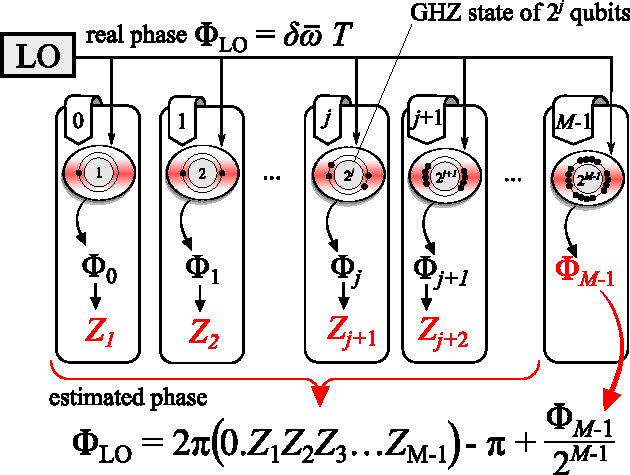
\includegraphics[width=0.8\textwidth]{./figs_Kessler2014/fig2.pdf}
\caption
[GHZ cascade]
{
\label{fig:phase_estimation}
The proposed clock operation scheme employs $M$ different groups of clock atoms
prepared in correlated states of varying size to interrogate the relative phase
$\Phi_\mathrm{LO}$ of the LO field.
A single group $j$ contains $n_0$ independent instances of GHZ-like states, each
entangling $2^j$ qubits, and therefore accumulating a phase $\Phi_j = 2^j
\Phi_\mathrm{LO} \mod [-\pi,\pi]$ during a single cycle. Each group is then used
to measure this phase, which gives a direct estimate on the digit $Z_{j+1}$ in a
binary representation of the LO phase
$(\Phi_\mathrm{LO}+\pi)/2\pi=(0.Z_1Z_2Z_3\hdots)$,
subsequently used to feedback the LO frequency.
}
\end{figure}

Let us assume, for the moment, that the accumulated laser phase after the
interrogation time $T$ lies in the interval $\Phi_\mathrm{LO}\in[-\pi,\pi)$, and
has an exact binary representation $(\Phi_\mathrm{LO}+\pi)/2\pi= \sum_{j=1}^M Z_j/
2^{j}$, with digits $Z_j\in \{0,1\}$ (both conditions will be relaxed below).
One can then readily show that a GHZ state consisting of $2^{M-1}$ atoms picks
up the phase $\Phi_{M-1} = 2^{M-1} \Phi_\mathrm{LO}  ~\mathrm{mod}~ [-\pi,\pi) = \pi
(Z_M-1)$. Thus, by measuring if the phase is $0$ or $\pi$, the last digit of the
laser phase can be determined. However, without
the remaining digits this information is
useless.
In our protocol, these digits are found by an additional, simultaneous
interrogation with successively smaller GHZ states of $2^{M-2},2^{M-3},\hdots$
entangled atoms (see \reffig{fig:phase_estimation}). Each of these states
picks up a phase proportional to its size  $\Phi_{j} = 2^{j}
\Phi_\mathrm{LO}~\mathrm{mod}~ [-\pi,\pi)$, and this
phase gets a contribution of $\pi (Z_j-1)$.
By distinguishing whether the phase is shifted by $\pi$ or not, we can 
determine the value of the bit $Z_j$.
The combined information provides an estimate with an accuracy given by the
largest GHZ state, while the cascade increases the total number of atoms
employed only by a factor of two: $\sum_{j=0}^{M-1} 2^j \approx
2^{M}=2\times2^{M-1}$.

However, in the limit of large averaging times, the assumption
$\Phi_\mathrm{LO}\in [-\pi,\pi)$ is not justified anymore. Here, the optimal
Ramsey time $T\sim\tau$ can attain values that induce phase wraps of the laser
itself, causing the binary representation of the laser phase to contain digits
$Z_j\neq0$ for $j\leq0$, which are inaccessible to the technique discussed
above.
To overcome this, we extend the cascade to
the classical domain, and employ additional groups of {\it uncorrelated}
atoms that interrogate the laser with successively decreasing interrogation times, or
alternatively, using dynamical decoupling techniques \cite{Rosenband2013,
Borregaard2013,ddc}. Each of these ensembles acquires a phase that is
reduced by multiples of two from the laser phase, and thus, following the
arguments from above, allows one to gain information on the digits
$Z_j$ with $j\leq0$.
The information of all digits combined provides the total number of phase wraps,
which in turn yields a Heisenberg-limited estimate of the laser phase.
By this, the protocol effectively eliminates all limitations
arising from the LO noise, and allows the Ramsey time to extend to its optimal
value.

 
% This paper is organized as follows. In Section~\ref{sec:EC} we provide an
% executive summary of the proposed clock operation scheme and the main results of
% our feedback analysis. This Section is self-contained, and can be read without
% consulting the following part of the paper.
% For the interested reader, the subsequent Sections provide the full details of
% our analysis. In Section $\hdots$

% It is a long standing view that GHZ-states cannot increase clock stability due
% to their increased susceptibility to phase slips in the presence of $1/f$-type
% local oscillator noise. \cite{Wineland1998}



%%%%%%%%%%%%%%%%%%%%%%%%%%%%%%%%%%%%%%%%%%%%%%%%%%%%%%%%%%%%%%%%%%%%%%%%%%%%%%%%%%5
%%%%%%%%%%%%%%%%%%%%%%%%%%%%%%%%%%%%%%%%%%%%%%%%%%%%%%%%%%%%%%%%%%%%%%%%%%%%%%%%%%5
\section{Feedback loop}
%%%%%%%%%%%%%%%%%%%%%%%%%%%%%%%%%%%%%%%%%%%%%%%%%%%%%%%%%%%%%%%%%%%%%%%%%%%%%%%%%%5
%%%%%%%%%%%%%%%%%%%%%%%%%%%%%%%%%%%%%%%%%%%%%%%%%%%%%%%%%%%%%%%%%%%%%%%%%%%%%%%%%%5
In the following, we provide a derivation of the above results
combined with feedback analysis that allows us to characterize
the achievable stability of a clock using our protocol. Modern
clocks periodically measure the fluctuating LO frequency $\omega(t)$ against the
frequency standard $\omega_0$ of the clock atoms to
obtain an error signal.
After each Ramsey cycle of duration $T$ [i.e., at times $t_k=kT$
($k=1,2\hdots$)], the measurement data yield
 an estimate of the relative phase, $\Phi_\mathrm{LO}(t_k) =
\int_{t_k-T}^{t_k}\d{t}[\omega(t) - \omega_0]$, accumulated by the LO.
This estimate in turn is used to readjust the frequency of the LO:  $\omega(t_k)
\rightarrow \omega(t_k) - \alpha\Phi^\mathrm{est}_\mathrm{LO}(t_k)/T$, where
$\Phi^\mathrm{est}_\mathrm{LO}(t_k)$ represents a suited estimator of the phase
$\Phi_\mathrm{LO}(t_k)$ \footnote{Alternatively, it is also possible to perform direct phase
feedback.}, and $\alpha < 1$ is an suitably chosen
gain.
%Phase feedback
%is chosen since it performs better in the presence of white noise
%\cite{Bollinger1996}, but one can use frequency
%feedback and achieve the same stability up to a constant factor.

The stability of the actively stabilized LO, after a total averaging time
$\tau$, is characterized by the Allan deviation (ADEV) which is directly
proportional to the measurement uncertainty $\Delta\Phi_\mathrm{LO}(t_k)$ after
each Ramsey cycle (see Appendix \ref{app:Kessler2014}),
\bel
	\label{eq:Allan-variance}
	\sigma_y(\tau) \equiv \frac{1}{\omega_0 \tau}
	\sqrt{\sum_{k = 1}^{\tau/T}\sum_{l = 1}^{\tau/T}
	T^2\ev{\delta\bar\omega_k\delta\bar\omega_l} }
	\approx
	 \frac{1}{\omega_0\sqrt{\tau T}} \Delta\Phi_\mathrm{LO}(T).
%  	 =
% 	\frac{1}{\omega_0^2\tau T} \frac{(\Delta\Phi_{M-1})^2}{D^{2M-2}}
% 	=:
% 	\frac{\gamma}{\omega_0^2 \tau} S^2(\gamma T,D,M,N)  ,
\eel
Here, $\delta\bar\omega_k = \Phi_\mathrm{LO}(t_k)/T$ is the average detuning of the
(stabilized) LO during the $k$th cycle. {%
 To obtain \refeq{eq:Allan-variance}, we use the fact that after the frequency
 feedback the detuning averages become approximately uncorrelated for realistic
 laser spectra, $\ev{\delta\bar\omega_k \delta\bar\omega_l} \approx
 \ev{\delta\bar\omega^2}\delta_{kl}$ \cite{Borregaard2013,
 Andre2005,Bloom2013}}.
%It has been shown that, if the frequency noise spectrum of the free running LO,
%$S_\omega(f)$, is less divergent than $\mathcal{O}(1/f^2)$ as  $f\rightarrow 0$,
%then the low-frequency part of the frequency noise spectrum of the actively
%stabilized LO $S^\mathrm{st}_\omega(f)$ is dominated by white noise originating
%entirely from measurement uncertainties \cite{Borregaard2013, Andre2005}.
%Since realistic laser noise spectra -- being dominated by white and $1/f$-noise
%(electronic flicker noise) \cite{Bishof2013} -- fulfill this condition,
%different Ramsey cycles are independent, and write the covariance as
%$\ev{\delta\bar\omega_k \delta\bar\omega_l} = \ev{\delta\bar\omega^2}\delta_{kl}
%= (\Delta \Phi_\mathrm{LO})^2\delta_{kl}/T^2$, which results in the right hand
 %side of \refeq{eq:Allan-variance}.
Other noise sources (such as the bias of the linear estimator, the Dick effect,
or a sub-optimal gain $\alpha$ \cite{Santarelli1998}) are not fundamental, and
neglected in the following.


%%%%%%%%%%%%%%%%%%%%%%%%%%%%%%%%%%%%%%%%%%%%%%%%%%%%%%%%%%%%%%%%%%%%%%%%%%%%%%%%%%5
%%%%%%%%%%%%%%%%%%%%%%%%%%%%%%%%%%%%%%%%%%%%%%%%%%%%%%%%%%%%%%%%%%%%%%%%%%%%%%%%%%5
\section{Spectroscopic nosies}
%%%%%%%%%%%%%%%%%%%%%%%%%%%%%%%%%%%%%%%%%%%%%%%%%%%%%%%%%%%%%%%%%%%%%%%%%%%%%%%%%%5
%%%%%%%%%%%%%%%%%%%%%%%%%%%%%%%%%%%%%%%%%%%%%%%%%%%%%%%%%%%%%%%%%%%%%%%%%%%%%%%%%%5

For small values of the accumulated Ramsey phase, the ultimate precision by
which this phase can be estimated is determined by the Cram\'{e}r-Rao bound
\cite{Rao1945,Giovanetti2011} which 
links the estimation error to the quantum Fisher information (QFI)
$\Delta\Phi_\mathrm{LO} \sim 1/\sqrt{\mathcal F}$ (for a review, see
\cite{Giovanetti2011}). The QFI, $\mathcal F$, is maximized, e.g., by the use of
GHZ states for which $\mathcal F \sim N^2$.
In clock stabilization, however, the LO frequency fluctuations account for the
fact that the accumulated Ramsey phase is a random variable which can obtain
large values, inherently violating the small phase assumption of the
Cram\'{e}r-Rao bound.
% A phase wrap error occurs whenever $\Phi(t_k)$ falls outside the interval
% $[-\pi,\pi)$ at the end of the $k$th cycle which can not be detected in a
% standard Ramsey measurement.
In particular for a single GHZ states, phase wraps of the atomic phase,
$\Phi(t_k)=N \Phi_\mathrm{LO}(t_k)\notin[-\pi,\pi)$, cannot be detected.
Consequently, the cycle time $T$ has to be
chosen such that the prior distribution of $\Phi(t_k)$ is well localized
within $[-\pi,\pi)$.
This limits the maximally allowed Ramsey time to a value $T_\mathrm{max}
\sim\gamma_\mathrm{LO}^{-1}/N^2$ (see 
Appendix \ref{app:Kessler2014}), where we assumed a white frequency noise
spectrum of the LO, $S_\omega(f) = \gamma_\mathrm{LO}$ (for $1/f$-noise one finds the less stringent
condition $T_\mathrm{max} \sim\gamma_\mathrm{LO}^{-1}/N$). In most cases, this value
lies below the optimal (i.e., maximal) value implied by
\refeq{eq:Allan-variance} $T\sim\tau$, resulting in a laser stability for GHZ
states which shows no improvement over the stability achieved with uncorrelated
atoms \cite{Wineland1998, Rosenband2012_numerical}.

However, unlike the individual particle noise resulting in the finite atom
linewidth $\gamma_\mathrm{ind}$, the LO frequency fluctuations affect all clock
atoms alike, and this \textit{collective noise} does not represent a fundamental
metrological limitation.
Ee can use a cascade of GHZ states of varying size to measure the
$\Phi_\mathrm{LO}$ in a binary representation, as discussed above.
In general, the phase does not have an exact binary representation ending at the
digit $Z_{M}$. We therefore employ $n_0$ duplicates  at each level of the
cascade (as opposed to sequential procedure suggested in \cite{Giovannetti2006})
($n_0 =N/\sum_{j=0}^{M-1} 2^j \approx N/2^M$) to improve the precision.
 In the case where all digits $Z_j$ ($j=1\dots, M-1$) are determined correctly
 according to the relation
\bel
Z_j =
[2(\Phi_{j-1}+\pi) - (\Phi_j + \pi)]/2\pi,
\eel
the last group ($j=M-1$) then yields a Heisenberg-limited estimate of
the LO phase with accuracy $(\Delta\Phi_\mathrm{LO})_\mathrm{pr} =
1/(2^{M-1} \sqrt{n_0}) = 2\sqrt{n_0}/N$.

%%%%%%%%%%%%%%%%%%%%%%%%%%%%%%%%%%%%%%%%%%%%%%%%%%%%%%%%%%%%%%%%%%%%%%%%%%%%%%%%%%5
%%%%%%%%%%%%%%%%%%%%%%%%%%%%%%%%%%%%%%%%%%%%%%%%%%%%%%%%%%%%%%%%%%%%%%%%%%%%%%%%%%5
\subsection{Phase estimation with multiple GHZ groups}
%%%%%%%%%%%%%%%%%%%%%%%%%%%%%%%%%%%%%%%%%%%%%%%%%%%%%%%%%%%%%%%%%%%%%%%%%%%%%%%%%%5
%%%%%%%%%%%%%%%%%%%%%%%%%%%%%%%%%%%%%%%%%%%%%%%%%%%%%%%%%%%%%%%%%%%%%%%%%%%%%%%%%%5
%{\it Cascaded GHZ.}---

%Let us assume for the moment that the prior distribution of the LO phase $\Phi_\mathrm{LO}$ after the
%Ramsey time is localized in $[-\pi,\pi)$ (we will relax this condition below), such that we can write $(\Phi_\mathrm{LO}+\pi)/
%2\pi= \sum_{j=1}^\infty Z_j/ 2^{j}\equiv0.Z_1Z_2Z_3\hdots$

%0.Z_1Z_2Z_3\hdots$. 
%Then we can
%represent the  phase we want to estimate as a binary fraction
%$(\Phi_\mathrm{LO}+\pi)/2\pi= \sum_{j=1}^\infty Z_j/ 2^{j}\equiv
%0.Z_1Z_2Z_3\hdots$, with digits $Z_j\in\{0,1\}$.


%We imagine dividing the $N$ qubits available into $M$ groups
%($j=0,1\dots M-1$), each containing $n_0$ independent instances of  $2^j$ number of
%qubits entangled in a GHZ state, $\ket{\mathbf{1}}_j + i \ket{\mathbf{0}}_j
%\equiv\ket{0}^{\otimes{2^j}} + i\ket{1}^{\otimes{2^j}}$ ($n_0 =
%N/\sum_{j=0}^{M-1} 2^j \approx N/2^M$), as shown in \reffig{fig:phase_estimation}.
 %Subsequently, the LO field is
% (with average detuning $\delta\bar\omega$)
%interrogated by all entangled states simultaneously  in a Ramsey cycle of length
%$T$, using the technique described in \cite{Bollinger1996}.
%After this interrogation the respective GHZ states are given as
%$\ket{\mathbf{1}}_j + i e^{i\Phi_j} \ket{\mathbf{0}}_j $ having accumulated the
%phase 
%\begin{align} \label{eq:EK1}
%\Phi_j =& 2^j \Phi_\mathrm{LO}  ~\mathrm{mod}~ [-\pi,\pi) \\ 
%=&2\pi 
%(0.Z_{j+1} Z_{j+2} Z_{j+3}\hdots)-\pi.
%\end{align}
%The largest group
%$j=M-1$ (i.e., the group with the fastest evolving GHZ states) consequently 
%can estimate $\Phi_{M-1} =2\pi  (0.Z_{M} Z_{M+1} \hdots)-\pi $ with accuracy
%$\Delta\Phi_{M-1} = 1/\sqrt{n_0} $ \cite{Itano1993,fn2}.
%The number of phase slips  $Z_1\hdots Z_{M-1}$ -- necessary to derive an estimate of the laser phase $\Phi_{LO}$ --  subsequently can be measured directly digit by digit from the groups of
%successively smaller GHZ states according to the relation 
%\bel
%Z_j =
%[2(\Phi_{j-1}+\pi) - (\Phi_j + \pi)]/2\pi
%.
%\eel If all digits $Z_j$ are determined correctly this yields a Heisenberg-limited estimate of
%the LO phase with accuracy $(\Delta\Phi_\mathrm{LO})_\mathrm{pr} =
%1/(2^{M-1} \sqrt{n_0}) = 2\sqrt{n_0}/N$, and with a Ramsey time that 
%can exceed the laser noise limit $T_\mathrm{max}$.

However, in general the estimation of the binary digits $Z_j$ is not perfect.
A rounding error occurs whenever $|\Phi_{j-1}^\mathrm{est} - \Phi_{j-1}| > \pi/2$
(where $\Phi_j^\mathrm{est}$ represents a suitable estimator derived from the $n_0$
measurement outcomes), leading to the wrong $Z_j$, and a variance contribution
of $(2\pi 2^{-j})^2$ for $\Phi_\mathrm{LO}$.
We can approximate their total
variance contribution with the sum
 $ 	(\Delta\Phi_\mathrm{LO})^2_\mathrm{re} = P_\mathrm{re}\sum_{j=1}^{M-1}
 	(2\pi 2^{-j})^2
%  	\frac{D}{\pi}\exp\left[-\frac{\pi^2}{D^2}n_0\right] 
%  	\approx 4\pi D^{2M-3}
%  	\exp\left[-\frac{\pi^2}{D^2}n_0\right].
 $, where 
$P_\mathrm{re} = 2\intop_{\pi/2}^{\infty}\d{\phi}
\rho(\phi)$, 
% \bel
% 	\label{eq:p_re}
% 	p_\mathrm{rounding error} = 2\intop_{\pi/2}^{\infty}\d{y} \rho(y) <
% 	2\intop_{\pi/2}^{\infty}\d{y} n_0 e^{-n_0y^2} 
% 	=
% 	\frac{2}{\pi}\exp\left[-\frac{\pi^2}{2^2}n_0\right] \left(1 +
% 	\mathcal{O}\left(\frac{2}{\pi}\right)\right), \qquad \forall j,
% \eel
and $\rho(\phi)$ is the Gaussian probability distribution of the error
$\Phi_j^\mathrm{est} - \Phi_j$ with a width proportional to $1/\sqrt n_0$  
(see Appendix \ref{app:Kessler2014}).
Consequently, rounding errors can be exponentially suppressed by choosing a
sufficiently large value for $n_0$. The total
measurement uncertainty of this estimation scheme is thus
$(\Delta\Phi_\mathrm{LO})^2 = (\Delta\Phi_\mathrm{LO})_\mathrm{pr}^2
+(\Delta\Phi_\mathrm{LO})_\mathrm{re}^2$.
In Appendix \ref{app:Kessler2014}, we show that the optimal allocation of
resources is achieved for the choice $n_{0}^{\mathrm{opt}} \sim
\frac{16}{\pi^2}\log\left(N\right)$, for which rounding errors are negligible,
yielding the total measurement accuracy
 \bel
 \label{eq:M}
\Delta\Phi_\mathrm{LO} \approx (\Delta\Phi_\mathrm{LO})_\mathrm{pr} =
\frac{8}{\pi}\sqrt{\mathrm{log}(N)}/N.
\eel This measurement precision obtains the Heisenberg limit (up to a
logarithmic correction resulting from the cost to suppress rounding errors)
despite it being applicable to a general (typically large) phase.

% \bel
% \tilde\Phi_j = (\Phi_j \mod [-\pi,\pi])= (D^j T\delta\bar\omega \mod
% [-\pi,\pi]),\qquad\qquad \Delta\tilde\Phi_j =
% \frac{1}{\sqrt{n_0}} \quad \forall j\qquad\mathrm{(from MLE)}
% \eel
% where $T$ is the free evolution time (See \reffig{fig:phase_estimation}).
% Its
% uncertainty is a good approximation
% % (strictly speaking, an upper bound) 
% of the uncertainty of $\Phi_\mathrm{LO}$, $\Delta\Phi_\mathrm{LO} =
% \Delta\Phi_{M-1}/D^{M-1}$.
% % \bel
% % 	\Delta\Phi_\mathrm{LO} = \frac{\Delta\Phi_{M-1}}{D^{M-1}}.
% % \eel
% Unfortunately, 

%Note, that this estimation protocol can be understood as an incoherent
%version of the phase estimation algorithm. However, as compared to previous versions of the latter \cite{Geza} the measurement uncertainty is
%reduced by a factor $ \propto 2^{M/2}/\sqrt{\mathrm{log}(N)}$ enabling the full
%quantum gain of our protocol.

So far we have assumed that $\Phi_\mathrm{LO}\in[-\pi,\pi)$ in each cycle.
However, for realistic laser noise spectra there is always a finite probability
that the LO phase $\Phi_\mathrm{LO}$ lies outside the interval $[-\pi,\pi)$ after
the interrogation time. Such phase wraps of the laser phase itself add to the
final measurement uncertainty in \refeq{eq:M} by the amount
$
	(\Delta\Phi_\mathrm{LO})^2_\mathrm{slip} =  (2\pi)^2P_\mathrm{slip}
$,
where 
$P_\mathrm{slip} = 2\intop_\pi^\infty \d{\phi} \rho_\mathrm{LO}(\phi)$,
% \bel
% 	\label{eq:p_slip}
% 	p_\mathrm{slip} = 2\intop_\pi^\infty \d{y} \rho_\mathrm{LO}(y) = 2\intop_\pi^\infty
% 	\d{y} \frac{1}{\sqrt{2\pi (\gamma T)^2}}
% 	\exp\left[-\frac{y^2}{2(\gamma T)^2}\right] = \sqrt{\frac{2}{\pi}}
% 	\frac{\gamma T}{\pi}\exp\left[-\frac{\pi^2}{2(\gamma T)^2}\right] \left(1
% 	+ \mathcal{O}\left(\frac{\gamma T}{\pi}\right)\right),
% \eel
and $\rho_\mathrm{LO}$ is the Gaussian prior distribution of $\Phi_\mathrm{LO}$.
Its width grows with $ \gamma_\mathrm{LO} T$, which puts a constraint on the
maximally allowed Ramsey time $T
\leq\frac{\pi^2}{4}\gamma_\mathrm{LO}^{-1}[\log(\gamma_\mathrm{LO}\tau N)]^{-1}$,
and thus the achievable ADEV $\sigma_y~(\propto 1/\sqrt T)$
 as we demonstrate in Appendix \ref{app:Kessler2014}.

This, however, does not represent a fundamental limitation as we can
extend the scheme by adding additional classical measurements with a shorter
Ramsey periods to assess the number of phase slips of
the laser phase itself $\hdots Z_{-3}Z_{-2}Z_{-1}Z_0$. As demonstrated in
Appendix \ref{app:Kessler2014}, this allows  extending the Ramsey time by a
factor $k$ adding only a negligible number of atoms $N^{*}\approx
\frac{8}{\pi^2} \log\left(k N^2\right)\log_2(k)\ll N$.
% This procedure can be understood as a classical pre-narrowing of the laser
% linewidth before the application of the quantum protocol.

% Using classical techniques the effective laser linewidth can be pre-narrowed
% before application of the proposed quantum protocol. This is achieved in a
% parallel interrogation with classical ensembles that measure the laser phase
% using varying Ramsey times, or alternatively, by employing dynamical
% decoupling techniques \cite{Rosenband2013, Borregaard2013,ddc}.
 % It allows the extension of the Ramsey time by a factor $k$ at negligible cost
 % in total resources $N^{*}\approx \frac{2}{\pi^2} D^2 \log\left(k
 % N^2\right)\log_D(k)\ll N$.
 % As we demonstrate in the SI, this can be understood as an extension of the
 % cascaded interrogation scheme to the classical domain to assess the binary
 % digits left of the point, $Z_j$ ($j<0$), eliminating the threat of
 % unaccounted phase slips of the laser phase.
 
% The Ramsey time is then only limited by individual noise processes resulting
% in the finite linewidth of the clock atoms $\gamma_\mathrm{ind}$ which put a
% fundamental limit on the allowed Ramsey time
% $T\leq\gamma_\mathrm{ind}^{-1}/2^{M-1}$, inversely proportional to the size of
% the GHZ states in group $M-1$.




%However, also here rounding errors do not represent a fundamental limitation. The necessity of using multiple copies $n_0$ can in principle be avoided by a quantum processing step of the clock atom state prior to the measurement. After the the interrogation time T the total state of the system is given as
%\begin{align}
%\Ket{\Psi} =\frac{1}{2^{M/2}}& \left( \Ket{\mathbf0}_0 + e^{i2^0\Phi_\mathrm{LO}}\Ket{\mathbf{1}}_0\right)\left( \Ket{\mathbf0}_1 + e^{i2^1\Phi_\mathrm{LO}}\Ket{\mathbf{1}}_1\right)\hdots\\
%&\left( \Ket{\mathbf0}_{M-1} + e^{i2^{M-1}\Phi_\mathrm{LO}}\Ket{\mathbf{1}}_{M-1}\right),
%\end{align}
%where we defined the logical qubits $\Ket{\mathbf0}_j = \Ket{0}^{\otimes 2^j}$ ($\Ket{\mathbf1}_j = \Ket{1}^{\otimes 2^j}$), according to the different GHZ groups. In the pathological case that $\phi_\mathrm{LO}$ has an exact $M$ bit binary representation, one readily shows that application of the inverse quantum Fourier transformation $U_\mathrm{QFT}^{-1}$ on the logical qubit state yields
%\bel
%U_\mathrm{QFT}^{-1} \Ket \Psi =\Ket{Z_1Z_2...Z_M},
%\eel
%such that a measurement of the logical qubits directly gives perfect information on $\phi_\mathrm{LO}$. Also in the general case of an arbitrary value of $\phi_\mathrm{LO}$, the measurement of the logical qubits in the computational basis yields an accurate estimate of the LO phase with uncertainty $(\Delta \Phi_\mathrm{LO})^2 \approx 2^{-2(M-1)}$. 

% Here, we note that the exponential dependence with $M$ translates to a
% polynomial dependence of $N$ after optimizing the value of $M$, which is
% then outweighed by the exponential scaling of $P_\mathrm{re}$. As a result, the
% noise from rounding errors is negligible compared to the projection noise at the
% optimal working point. 


%Although, individual atom dephasing affects negligibly the stability in the case
%of uncorrelated atoms, it
%contributes significantly for GHZ states with sufficiently large number of
%entangled atoms. This effect of this dephasing is increased by a factor of
%$2^{M-1}$  on the $j=M-1$ group, compared to the uncorrelated group ($j=0$),
%yielding the variance contribution
%\bel
%	(\Delta\Phi_{M-1})^2_\mathrm{ind} = 2^{M-1}\frac{\gamma_\mathrm{ind}T}{n_0},
%\eel
%where $\gamma_\mathrm{ind}$ is the atomic linewidth. 
% 	\sqrt{\frac{2}{\pi}} \frac{\gamma T}{\pi}\exp\left[-\frac{\pi^2}{2(\gamma
% T)^2}\right].
%The full variance of  $\Phi_{M-1}$ is given as the
%sum, $(\Delta\Phi_{M-1})^2 = (\Delta\Phi_{M-1})^2_\mathrm{pr} +
%(\Delta\Phi_{M-1})^2_\mathrm{re} + (\Delta\Phi_{M-1})^2_\mathrm{slip} +
%(\Delta\Phi_{M-1})^2_\mathrm{ind}$, assuming $P_\mathrm{re}, P_\mathrm{slip} \ll 1$. 
% Finally
% $\mathrm{Var}(\Phi_\mathrm{LO}) = \frac{(\Delta\Phi_{M-1})^2}{D^{2M-2}}$.
% \bel
% 	(\Delta\Phi_{M-1})^2 = ([\Delta\Phi_{M-1}]_\mathrm{pr})^2 +
% 	([\Delta\Phi_{M-1}]_\mathrm{re})^2 + ([\Delta\Phi_{M-1}]_\mathrm{slip})^2.
% \eel


%%%%%%%%%%%%%%%%%%%%%%%%%%%%%%%%%%%%%%%%%%%%%%%%%%%%%%%%%%%%%%%%%%%%%%%%%%%%%%%%%%5
%%%%%%%%%%%%%%%%%%%%%%%%%%%%%%%%%%%%%%%%%%%%%%%%%%%%%%%%%%%%%%%%%%%%%%%%%%%%%%%%%%5
\subsection{Optimization}
%%%%%%%%%%%%%%%%%%%%%%%%%%%%%%%%%%%%%%%%%%%%%%%%%%%%%%%%%%%%%%%%%%%%%%%%%%%%%%%%%%5
%%%%%%%%%%%%%%%%%%%%%%%%%%%%%%%%%%%%%%%%%%%%%%%%%%%%%%%%%%%%%%%%%%%%%%%%%%%%%%%%%%5
With all phase wraps counted correctly, the Ramsey time is only limited by
individual noise processes. The finite linewidth of the atomic clock transition
$\gamma_\mathrm{ind}$ gives rise to the fundamental constraint
$T\leq\gamma_\mathrm{ind}^{-1}/2^{M-1}$.
For averaging times
$\tau\leq\gamma_\mathrm{ind}^{-1}/2^{M-1}$, we can choose $T \approx \tau$, and
using the optimized value for $n_0$ found above the resulting clock stability is
obtained from \refeq{eq:Allan-variance}
\bel
	\label{eq:sigma(1)}
	\sigma_y(\tau)^{(1)} \approx	
	%\frac{1}{\omega_0\tau}
	%\frac{1}{\sqrt{n_{0,\mathrm{opt}}} 2^{M-1}}=
	\frac{2}{\omega_0\tau}
	\frac{\sqrt{n_{0}^{\mathrm{opt}}}}{N} \approx	\frac{8}{\pi\omega_0\tau}
	\frac{\sqrt{\mathrm{log}(N)}}{N}.
\eel
It scales linearly with the averaging time $\tau$, and realizes the Heisenberg
bound of laser stability up to a logarithmic correction. In contrast, in the regime $\tau\geq\gamma_\mathrm{ind}^{-1}/2^{M-1}$, $T$ is limited
by the presence of individual particle noise to a value $T\approx \gamma_\mathrm{ind}^{-1}/2^{M-1}= 2 \gamma_\mathrm{ind}^{-1}n_0/N$, and we find
\bel
	\label{eq:sigma(2)}
	\sigma_y(\tau)^{(2)} \approx
	\frac{1}{\omega_0}  \sqrt{\frac{\gamma_\mathrm{ind}}{\tau N}}.
\eel
\refeq{eq:sigma(2)} represents the fundamental noise floor for laser stability
resulting from quantum metrological bounds in the presence of individual
particle noise \cite{Escher:2011fn}. As we have seen, the proposed protocol
reaches this optimal value rapidly after the averaging time $\tau_0 \sim  
\gamma_\mathrm{ind}^{-1} \mathrm{log}(N)/N$ (cf. \reffig{fig:sigma_tau}),
$N/\mathrm{log}(N)$ times faster than any classical scheme.
In Appendix \ref{app:Kessler2014} we derive the necessary threshold fidelities in
the GHZ state preparation our scheme can tolerate without compromising the stability
in Eqs.~(\ref{eq:sigma(1)}) \& (\ref{eq:sigma(2)}).

\begin{figure}
\centering 
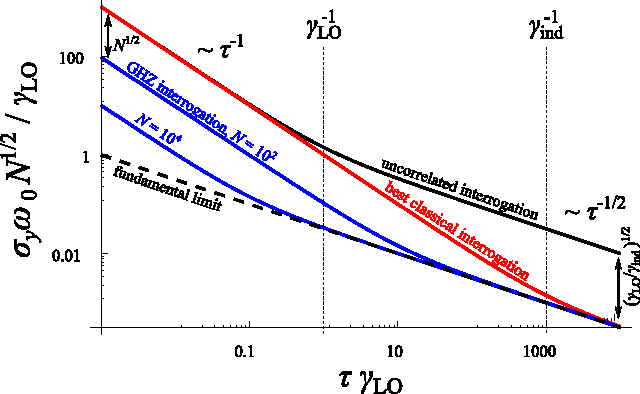
\includegraphics[width=0.9\textwidth]{./figs_Kessler2014/fig1.pdf}
\caption
[Comparison of clock protocols] 
{
\label{fig:sigma_tau}
Allan deviation $\sigma_y$ for different protocols as a function of averaging
time $\tau$, normalized to the standard quantum limit, for $\gamma_\mathrm{LO} /
\gamma_\mathrm{ind} = 10^3$. The solid black line corresponds to the standard scheme using
a single uncorrelated ensemble. It fails to reach the fundamental noise floor
set by the atomic transition linewidth (cf. \refeq{eq:sigma(2)}, broken line).
A more sophisticated classical scheme which uses exponentially increasing Ramsey
times in each cycle \cite{Rosenband2013, Borregaard2013} allows to extend the
regime of linear scaling with $1/\tau$ up to the point where the bound
(\ref{eq:sigma(2)}) is met. In comparison, the proposed cascaded GHZ protocol
(blue solid curves) enables an $\sim N$ times faster convergence. For short
averaging times the stability is enhanced by a factor $\sqrt{N}$ as compared to
classical protocols.
}
\end{figure} 


% 
% , where
% \bel
% 	\label{eq:S^2}
% 	S^2(\gamma T,C) = \frac{1}{\gamma T} C 
% 	+ \sqrt{32\pi}	\exp\left[-\frac{\pi^2}{2(\gamma T)^2}\right],
% \eel
% and
% \bel
% 	\label{eq:C}
% 	C(D,M,N) = \frac{1}{N D^{M-1}} +
% 	\frac{8\pi
% 	N^{1/2}}{D^{\frac{M+1}{2}}}\exp\left[-\frac{\pi^2 N}{2D^{M+1}}\right],
% \eel
% which can be obtain by approximating the
% integrals of the Gaussians with the first term of the asymptotic series,
%  $\int_x^\infty \d{\xi}\exp[-\xi^2/2] = \exp[-x^2/2]\left(1/x +
% \mathcal{O}(x^{-2})\right)$, and assuming $\sum_{j=0}^{M-1}D^j \approx D^{M-1}$.
% % Appendix \ref{sec:Optimization} contains the details of carrying out the
% % optimization.
% 
% The highest stability is achieved for the minimal $S^2$, which can be found by
% direct optimization, which we carry out in three steps.
% First, we find $\gamma T_\mathrm{opt}$ in terms of $C$, by finding the global
% minimum of \refeq{eq:S^2} analytically, in the limit $\gamma T \ll 1$, using the
% general solution of the transcendental equation $x^n = A\exp[-1/x]$ in the case
% of $A\gg 1$ (see Supplementary Materials).
% This yields $\gamma T_\mathrm{opt} =
% \frac{\pi}{\sqrt{2}}\left[\log\frac{8\pi^{3/2}}{C}\right]^{-1/2}$.
% The resulting function $S^2( \gamma T_\mathrm{opt}(C), C)$ is monotonically
% decreasing for $C \ll 1$, which is the relevant region for us.
% In the second step, we find $D_\mathrm{opt}$ in terms of $M$ and $N$ by finding
% the global minimum of \refeq{eq:C} analytically in the limit $N/D^{M+1} \gg 1$,
% using the same technique.
%%%%%%%%%%%%%%%%%%%%%%%%%%%%%%%%%%%%%%%%%%%%%%%%%%%%%%%%%%%%%%%%%%%%%%%%%%%%%%%%%%5
%%%%%%%%%%%%%%%%%%%%%%%%%%%%%%%%%%%%%%%%%%%%%%%%%%%%%%%%%%%%%%%%%%%%%%%%%%%%%%%%%%5
%\section{Different timescales}
\section{Comparison with other schemes}
%%%%%%%%%%%%%%%%%%%%%%%%%%%%%%%%%%%%%%%%%%%%%%%%%%%%%%%%%%%%%%%%%%%%%%%%%%%%%%%%%%5
%%%%%%%%%%%%%%%%%%%%%%%%%%%%%%%%%%%%%%%%%%%%%%%%%%%%%%%%%%%%%%%%%%%%%%%%%%%%%%%%%%5
%{\it Comparison with other schemes.}---
In the following, we benchmark the stability of our protocol against different approaches by
comparing the lowest achievable ADEV as a function of averaging
time $\tau$ (cf. \reffig{fig:sigma_tau}). 
First, we consider the standard procedure in which all atoms are interrogated
in an uncorrelated fashion. The scheme is identical to $N$
independent measurements of $\Phi_\mathrm{LO}$, and therefore the  ADEV
is limited by the standard quantum limit: $\sigma_y \sim \frac{1}{\omega_0
\tau\sqrt{N}}$ for $\tau < \gamma_\mathrm{LO}^{-1}$.
Since the Ramsey time is limited, by the LO noise, to $T<\gamma_\mathrm{LO}^{-1}$
due to uncorrected phase wraps, this fails to achieve the
fundamental bound, \refeq{eq:sigma(2)}, giving suboptimal ADEV,
  $\sigma_y(\tau) \sim
\frac{1}{\omega_0}\sqrt{\frac{\gamma_\mathrm{LO}}{\tau N}}$, in the long time
limit $ \tau > \gamma_\mathrm{LO}^{-1}$.
Second, we discuss the recently published classical protocol which
interrogates the LO with uncorrelated atoms for exponentially increasing Ramsey
times in each cycle \cite{Borregaard2013, Rosenband2013}. This protocol can be
understood as the classical part ($j\leq0$) of the cascaded interrogation
proposed here .
It eliminates the constraint of the LO linewidth, and allows to extend the interrogation time $T$ to its maximum value, enabling a linear scaling with $\tau$ up to the point where the fundamental bound
(\ref{eq:sigma(2)}) is reached.
However, using an uncorrelated interrogation, the scheme displays a standard-quantum-limited scaling (i.e.
$\propto1/\sqrt{N}$), for short averaging times. 
 
The above analysis illustrates the quantum gain of the proposed clock
operation protocol using cascaded GHZ states. As compared to the best known
classical scheme, our scheme provides a $\sqrt{N/\mathrm{log}(N)}$ enhancement for
short averaging times. As a result it reaches the fundamental noise floor for
laser stability in the presence of single particle decoherence
[\refeq{eq:sigma(2)}] $\sim N/{\mathrm{log}(N)}$ times faster.
This results identifies the possible advantage of using entanglement
previously debated in the literature
\cite{Wineland1998,Huelga1997,LouchetChauvet:2010fs,Rosenband2012_numerical,Borregaard2013_nearHeisenberg,Andre2004,Buzek1999,Meiser:2008fo}:
While the long term limitation is set by atomic decoherence, entangled atoms
reaches this limit faster thus improving the bandwidth of the stable oscillator.
Our results motivate the development of quantum enhanced atomic clocks based on entangled ions
and neutral atoms. Furthermore, it lays the foundations for the recently proposed network of quantum clocks \cite{Komar2014}
which achieves the optimal use of resources in a global network through
network-wide entangled states.

 
\chapter{A quantum network of clocks}
\label{ch:Komar2014}
%From \cite{Komar2014}
%%%%%%%%%%%%%%%%%%%%%%%%%%%%%%%%%%%%%%%%%%%%%%%%

\section{Introduction}

The development of precise atomic clocks 
% has led to many scientific and
% technological advances that 
plays an  increasingly important role in  modern
society. Shared timing information constitutes a key resource for  
% positioning and 
navigation with a direct correspondence between timing accuracy and
precision in applications such as the Global Positioning System (GPS).
By combining  precision metrology and quantum networks, we propose 
% here 
a
quantum, cooperative protocol for operating a network of
geographically remote optical atomic clocks. Using non-local entangled states,
we demonstrate an optimal utilization of 
% the 
global 
% network 
resources, and show
that such a network can be operated near the fundamental precision limit set by
quantum theory.
Furthermore, the internal structure of the network, combined with 
% basic
quantum communication techniques, guarantees security both from internal
and external threats. Realization of such a global quantum network of clocks may
allow construction of a real-time single international time scale (world clock)
with unprecedented stability and accuracy.

 
With the advances of highly phase coherent lasers, optical atomic clocks
containing multiple atoms have demonstrated stability that reaches the standard
quantum limit (SQL) set by the available atom number 
% within a clock 
and interrogation time
\cite{Bloom2013, Hinkley2013, Nicholson2012}.
Reaching beyond the SQL, we stand to gain a significant improvement of clock
performance by preparing atoms in quantum correlated states (e.g., spin squeezed
states \cite{Leroux2010, Buzek1999}). Here we describe a new
approach to maximize the performance of a network composed of multiple clocks allowing one to gain the
advantage of all resources available at each node.
Several recent advances in precision metrology and quantum science,
along with future improvements in quantum control,  
may put this
approach within reach.  On the
 one hand, 
%  capabilities to maintain 
 phase coherent
optical links spanning the entire visible spectrum 
% and over macroscopic distances 
have been demonstrated, with the capability of delivering the most
stable optical oscillator from one color or location to another \cite{Ye2003,
Droste2013}.
On the other hand, quantum communication and entanglement techniques are
enabling distant quantum objects to be connected in a quantum network
\cite{cirac, kimble, acin}.
% , that can enable novel,
% extraordinary capabilities.
Combining these two technological frontiers, we show here that  a distributed
network composed of quantum-limited clocks separated by large distances -- as
appropriate, e.g., for satellite-based clocks possibly operated by different
nations -- can be operated  as an ultimate ``world clock'', where all members
combine their individual resources in a quantum coherent way  to achieve greater
clock stability and distribute this international time scale in real time for
all. 

The distributed architecture allows each participant of the network to profit
from a stability of the local clock signal that is enhanced by a factor
proportional to the total number of parties (as compared to an independent
operation of the individual clocks) without losing sovereignty or compromising
security. This cooperative gain strongly incentivizes joining the collaborative
network while retaining robustness against
 disruptions of communication channels.
%  by allowing the parties to fall back to
%  individual clock operation.
% Our scheme can be superior to an alternative approach of disseminating the time
% signal from a single location containing all qubits. 
On the one hand,
the local clocks can be used to identify and correct systematic errors
origination from the phase links. On the other hand, the nodes can fall
back to relying on the locally stabilized clocks if the phase links fail.
% since errors arising from imperfect phase links can be largely reduced by
% relying on the stabilized and locally available local oscillators.
% Our scheme is superior to an alternative approach of disseminating the time
% signal from a single location containing all qubits since, for short times,
% unavoidable fluctuations of the required phase stabilized links cancel the
% quantum gain. 
We demonstrate that by preparing quantum-correlated states of
remote clocks, the network can yield the best possible clock signal allowed by
quantum theory for the combined resources.
Furthermore, enabled through the use of quantum communication techniques,  such
a network can be made secure, such that only parties contributing to its
operation may enjoy the benefit of an ultra-precise clock signal. Besides
serving as a real-time clock for the international time scale,  the proposed
quantum network also represents a large-scale quantum sensor that can be used to
probe the fundamental laws of physics, including relativity and connections between space-time and quantum physics.

  










\section{The concept of quantum clock network}
\label{sec:QCN}

\reffig{fig:1} illustrates the basic concept for the proposed quantum
clock network.
We consider a set of $K$ atomic clocks (constituting the nodes of the network), each based on a large number of atoms (clock
qubits) serving as the frequency reference $\omega_0$ at different geographical
locations. In our approach,  each clock has its own independently operated local
oscillator (LO), $\mathcal{E}_j(t)\propto e^{i\nu_j t}$, with detuning $\delta_j
= \nu_j - \omega_0$, $(j=1,2\dots K)$. It keeps the time by interrogating its
qubits periodically, and uses the measurement data to stabilize the LO frequency
at the reference frequency of the atomic transition. However, as opposed to the
conventional approach, 
% in which each LO interrogates its own independent qubits,
we consider the situation in which each network node  allocates some of its
qubits to form entangled states stretching across all nodes. When interrogated
within a properly designed measurement scheme, such entangled network states
provide ultra-precise information about the deviation of the center-of-mass
(COM) frequency $\nu_\textrm{COM} = \sum_j \nu_j/K$ of all local oscillators
from the atomic resonance.  
\begin{figure}
\centering
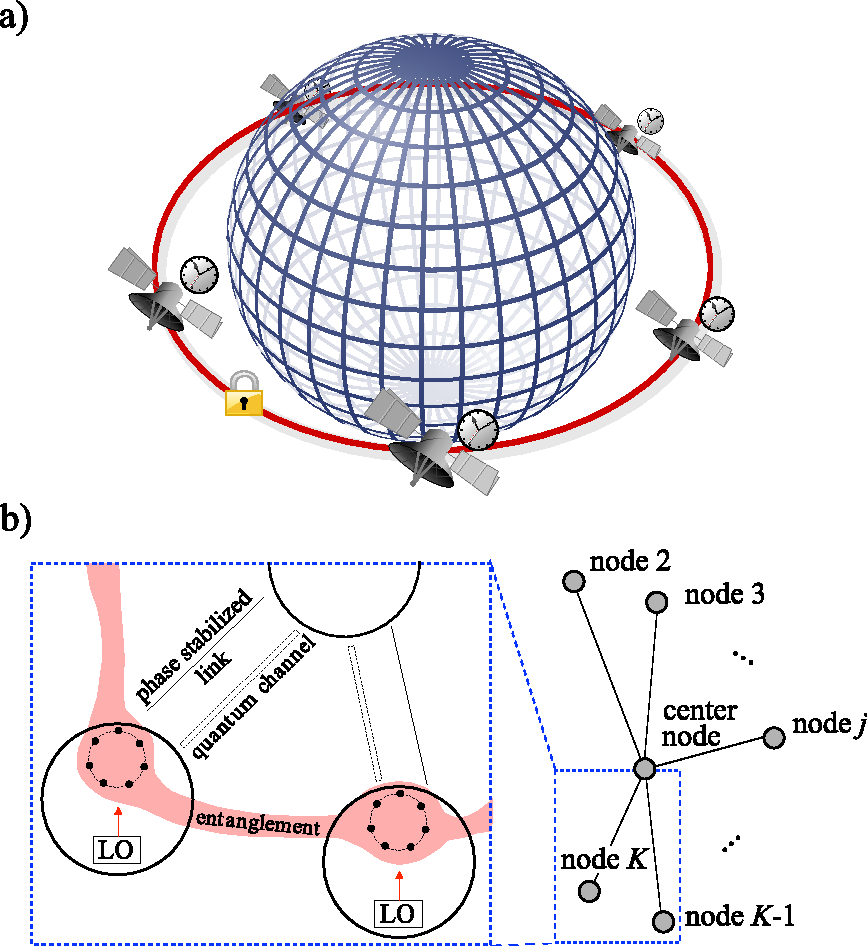
\includegraphics[width=0.8\textwidth]{./figs_Komar2014/fig1.pdf}
\caption
[The concept of world-wide quantum clock network]
{
\label{fig:1} The concept of world-wide quantum clock network.
a) Illustration of a cooperative clock operation protocol in which individual parties (e.g., satellite based atomic clocks from different countries) jointly allocate
their respective resources in a global network involving entangled quantum states. This guarantees an
optimal use of the global resources, achieving an ultra-precise clock signal
limited only by the fundamental bounds of quantum metrology and,
in addition, guaranteeing secure distribution of the clock signal.
 b) In addition to locally operating the individual clocks, the different nodes
 (i.e., satellites) employ network-wide entangled states to interrogate their
 respective local oscillators (LOs). The acquired information is sent to a particular node serving as
 a center where it is used to stabilize a center of mass mode of the different
 LOs. This yields an ultra-precise clock signal accessible to all network
 members.}
\end{figure}




% In the following, we describe the general working
% principle of  the proposed quantum clock network.



Each clock cycle consists of three stages: preparation of the clock atom state
(initialization), interrogation by the LOs (measurement) and correction of the
laser frequency according to the measurement outcome (feedback).
In the further analysis, we assume, for convenience, that in each interrogation
cycle one of the nodes plays the role of the center, which initiates
each Ramsey cycle and collects the measurement data from the other nodes via
classical channels [\reffig{fig:1}~b)], as well as LO signals via optical links,
 to feedback the COM signal.
(The role of the center can alternate to provide extra security, see
 Supplementary Information). This information, in turn, can be utilized in a feedback cycle to yield a Heisenberg-limited
stability of the COM clock signal generated by the network, which is 
subsequently distributed to the individual nodes in a secure fashion.  As a
result, after a few cycles, the LOs corresponding to each individual node
achieve an accuracy and stability effectively resulting from interrogating atoms
in the entire network.



\section{Preparation of network-wide entangled states}
\label{sec:NWES}

In the initialization stage of each clock cycle, entangled states spanning
across the nodes at different geographical positions of the network are
prepared. In the following, we describe exemplarily how a single network-wide
GHZ state can be prepared. 
The entangled states employed in the proposed quantum network protocol -- which
is described in the following section -- consist of products of GHZ states of
different size. They can be prepared by repetition of the protocol that
we now describe.

For simplicity, we assume that each node $j$ ($j=1,\dots K$) contains an
identical number $n$ of clock qubits which we label as $1_j, 2_j,\dots n_j$ (in
the Supplementary Information we discuss the case where the nodes contain
different amounts of clock qubits).
Further, we assume, for convenience, that the center node ($j=1$) has access to
additional $2(K-1)$ ancilla qubits $a_2,\dots, a_K,b_2,\dots,b_K$ besides the
$n$ clock atoms (a slightly more complicated procedure allows to refrain from
the use of ancilla qubits, see Supplementary Information).
The entangling procedure starts at the center with the creation of a fully
entangled state of one half of the ancilla qubits $\{b_j\}$, and its first clock
qubit $1_1$. 
This can be realized, e.g.  with a single qubit $\pi/2$-rotation
(on qubit $1_1$)
and a collective entangling operation, which is equivalent to a series of
CNOT gates \cite{Nielsen_Chuang} (between $1_1$ and each $b_j$).
The result is a GHZ state, $[\ket{00\dots 0}_{1_1,b_2,b_3,\dots b_K} +
i\ket{11\dots 1}_{1_1,b_2,b_3,\dots b_K}]/\sqrt{2}$.
%performed with the local oscillator field at the center, $\mathcal{E}_1$. 
% \bel
% 	\ket{00\dots 0}_{c_1,c_2\dots c_K} \quad\rightarrow\quad \frac{\ket{0}_1 +
% 	i\ket{1}_1}{\sqrt{2}} \ket{0\dots 0}_{2\dots M} \quad\rightarrow\quad
% 	\frac{\ket{00\dots 0}_{1,2\dots M} + i\ket{11\dots 1}_{1,2\dots M}}{\sqrt{2}},
% \eel
In parallel, the center uses the other half of the ancillas $\{a_j\}$ to create single EPR pairs with each node $j\neq1$,
either by directly sending flying qubits and converting them to stationary
qubits, or by using quantum repeater techniques to prepare high-fidelity entanglement \cite{duan3}. As a result of this procedure, 
one part of the pair is stored at the center node (qubit $a_j$), while the other one
is stored at the $j$th  node (qubit $1_j$), forming the states $[\ket{00}_{a_j,1_j} +
\ket{11}_{a_j,1_j}]/\sqrt{2}$ for every $j$ (see \reffig{fig:entangling}).
\begin{figure}
\centering
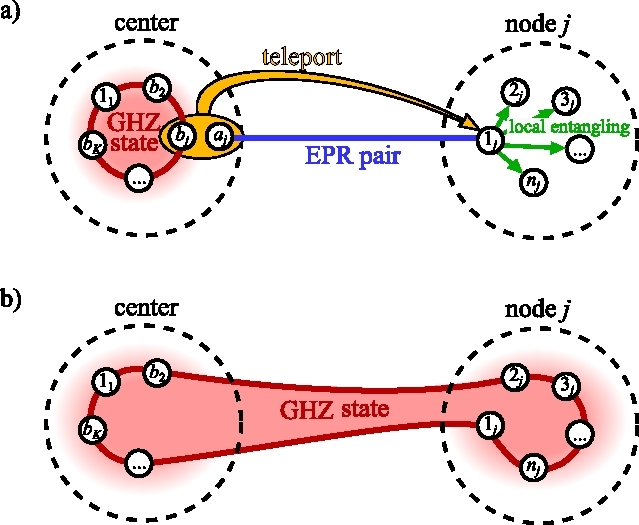
\includegraphics[width=0.7\textwidth]{./figs_Komar2014/fig2.pdf}
\caption
[Entangled state preparation between distant nodes]
{
\label{fig:entangling}
Entangled state preparation between distant nodes.
a) The center node $(j=1)$ initiates the initialization sequence by preparing a
local GHZ state across the qubits $\{b_j\}_{j=2}^K$ and $1_1$, as well as $(K-1)$ EPR pairs on
the qubit pairs $\{(a_j,1_j)\}_{j=2}^K$.
Quantum teleportation expands this GHZ state to the first qubit within each of
the individual nodes.
b) Originating from the teleported qubits, the nodes grow the GHZ state to
involve all the desired local qubits by employing local entangling
operations.
The procedure results in a common GHZ states over all atoms of the nodes.
 }
\end{figure}


%\subsection{Entangling}
% based on the existence of a secure central
% station,
Next, the center performs $K-1$ separate Bell measurements on
 its ancilla qubit pairs $\{(b_j, a_j)\}$. This teleports the state of qubit $b_j$ to
 qubit $1_j$
($j=2,\dots K$), up to a local single-qubit rotation, which is performed
after the measurement outcomes are sent to the node via classical channels.
The result of the  teleportations is a collective GHZ state
$\frac{1}{\sqrt{2}}\ket{00\dots 0}_{1_1,1_2,\dots 1_K} + i \ket{11\dots
1}_{1_1,1_2,\dots 1_K}$, stretching across the first qubits of all $K$ nodes.

In the final step of entangling, all nodes (including the center) extend the
entanglement to all of their remaining clock qubits. To do this, each node $j$
performs the collective entangling operation mentioned before based on
$1_j$ and targeting qubits $2_j, 3_j, \dots n_j$.  At the end of the protocol the different nodes share a common
GHZ state $[\ket{\mathbf{0}} + i\ket{\mathbf{1}}]/\sqrt{2}$, where
$\ket{\mathbf{0}}$ and $\ket{\mathbf{1}}$ are product states of all qubits
$\{i_j\;:\; i=1,2,\dots n,\; j=1,2,\dots K\}$ being in $\ket{0}$ or $\ket{1}$,
respectively. As discussed below, in practice the entanglement distribution can
be done  either via polarization- or frequency-entangled photons with frequency
difference in the microwave domain, in which case the ancillary qubits involved
in the entanglement distribution will be different from the clock qubits.
Typically, as part of the preparation process, time delays arise between the
initialization of different clock qubits. Its detrimental effects can be
entirely avoided by proper local timing or prior preparation of entanglement, as
discussed in the Supplementary Information.

\section{Interrogation}
\label{sec:SA}


The use of entangled resources 
% (in form of network-wide GHZ-like states) 
during
the interrogation phase enables an optimal use of the available resources via
the following procedure.  Assume we have a total of $\tilde N$ 
%($M$ being a positive integer)
qubits at
our disposal which are equally distributed between the $K$ nodes (indexed
$j=1,\hdots K$) and prepared in a non-local GHZ state $[\ket{\mathbf{0}} +
i\ket{\mathbf{1}}]/\sqrt{2}$, where $\ket{\mathbf{0 (1)}}\equiv\ket{0(1)}^{\otimes
\tilde N}$. During the
interrogation time $T$, a clock qubit at node $j$ picks up a relative phase $\phi_j = \delta_j
T$.
Due to the non-local character of the state, these phases accumulate in the total
state of the atoms  $[\ket{\mathbf{0}} + i e^{i\Phi}\ket{\mathbf{1}}]/\sqrt{2}$,
where the collective phase after the interrogation time $T$ is given as
\bel
\label{eq:1}
\Phi = \sum_{j=1}^K \frac{\tilde N}{K} \phi_j =
\tilde N \delta_\mathrm{COM} T,
\eel
where $\delta_\mathrm{COM} = \nu_\mathrm{COM} - \omega_0$.
% \bel
% 	\frac{1}{\sqrt{2}} \big(\ket{\mathbf{0}} + i
% 	e^{i\Phi}\ket{\mathbf{1}}),\qquad \Phi = \sum_{k=1}^M N_k \delta_k T .
% \eel
% This phase, $\Phi$, is sensitive to the weighted average of the detunings, ie.
% the center of mass of the detunings, $\nu_\mathrm{COM}-\omega_0 =
% \delta_\mathrm{COM} = [\sum N_k \delta_k] / [\sum N_k]$. By designing a
% measurement scheme estimating $\Phi$, we can get information on this COM
% detuning.
To extract the phase information picked up by the different GHZ states, 
% after each interrogation phase, 
the individual nodes $j$ measure their respective
qubits in the $x$-basis, and evaluate the parity of all measurement outcomes
$p_j$.
Subsequently, the nodes send this information to the center node via a classical
channel, where the total parity $p = \prod_{j} p_{j}$ is evaluated, and the
phase information is extracted \cite{Bollinger1996, Leibfried2004}. Note, that
only the full set $\{p_j |j=1\hdots K \}$ contains information. 
% This can be
% interpreted as only the center node holding the key,  namely its own measurement
% outcome $p_1$, to decode the phase information sent from the nodes.

The proportionality with $\tilde N$ in \refeq{eq:1} represents the quantum
enhancement in the estimation of $\delta_\mathrm{COM}$. However, for realistic
laser noise spectra, this suggested enhancement is corrupted  by the increase of
uncontrolled phase slips for a single GHZ
state 
%(i.e., undetectable transitions between fringes in a Ramsey
%experiment) 
\cite{Wineland1998}: Whenever, after the Ramsey time $T$, the phase $\Phi$ --
which due to the laser frequency fluctuations constitutes a random variable itself --
falls out of the interval $[-\pi,\pi]$ the estimation fails. This limitation
restricts the maximal Ramsey time to values $T < (\tilde
N\gamma_\mathrm{LO})^{-1}$, preventing any quantum gain in the estimation.


To circumvent this problem, we use entangled states consisting of products of
successively larger GHZ ensembles, see SI and 
\cite{Kessler2014}. In this approach, 
% interrogated network 
atoms are split into
several independent, shared groups.
% enables to correct for laser phase slips and 
%restores the quantum
%enhancement [REF:PRL paper]. 
% In the following, we apply these ideas to the clock network
% described above.
We write the number of the first group of atoms as $\tilde N =2^{M-1} K$, for
some natural number $M$.
Furthermore, the network shares additional groups of atoms, each containing
$2^{j} K$ ($j=0, \hdots M-2$) equally distributed between the nodes and prepared
in GHZ states. 
% \pk{The state of all the qubits can be written as
% $\left(\prod_{j=0}^{M-1} [\ket{0}^{2^jK} +
% i\ket{1}^{2^jK}]/\sqrt{2}\right)^{n_0}$, where $n_0$ is a small integer.}
Additionally, each node has a small number of uncorrelated atoms interrogated by
the LOs. Using a protocol reminiscent of the phase estimation algorithm
\cite{Kessler2014,Nielsen_Chuang, Giedke2006}, measurement results from each
level $j$ allow to directly assess the bits $Z_j \in \{0,1\}$ of the binary
fraction representation of the laser phase $\Phi_\mathrm{LO}=\delta_\mathrm{COM} T
=2\pi [(Z_1-1) 2^{-1} + Z_2 2^{-2} + Z_3 2^{-3} \hdots]$.
(See SI, section I.B for details.)
This
% accounts for all phase slips {\it what does this mean?? up to the uncorrelated
% ensemble}, and
yields an estimate of $\Phi_\mathrm{LO}$ with Heisenberg-limited accuracy, up to a
logarithmic correction, see SI:
\bel 
	\Delta \Phi_\mathrm{LO} =\frac{8}{\pi}\log(N)/N,
	\label{eq2}
\eel 
even for Ramsey times beyond the limits of the laser frequency fluctuations [$T
> (\tilde N\gamma_\mathrm{LO}^{-1})$], where $N$ represent the total number of
clock atoms employed in the scheme. The logarithmic correction arises due to the
number of particles required to realize this (incoherent) version of the phase
estimation algorithm.

\section{Feedback}

The measured value of the phase  $\Phi_\mathrm{LO}$,
gives an estimate on the COM detuning
$\tilde\delta_\mathrm{COM}$ after each Ramsey cycle, which is subsequently used
by the center node to stabilize the COM laser signal.
To this end, the center generates the COM of the frequencies. Every node sends
its local oscillator field $\mathcal{E}_i$ to the center via phase-stable
optical links, and the center synthesizes the COM frequency $\nu_\mathrm{COM}$ by
averaging the $\nu_j$ frequencies with equal weights.
% \footnote{With different
% number of qubits at each node, the weighted average needs to be taken.}
This can be implemented via heterodyne beat of the local oscillator in the
center against each incoming laser signal, resulting in $K$ beat frequencies.
Synthesizing  these beat frequencies allows the
local oscillator of the central node to phase track $\nu_\mathrm{COM}$.
%Subsequently, the center uses the 
%acquired information about $\delta_\mathrm{COM}$ to stabilize $\nu_\mathrm{COM}$ by
%application of digital frequency shifts. 
The center distributes the stabilized clock signal to different members of the network by sending individual error
signals $\tilde \delta_j = \tilde \delta_\mathrm{COM} + (\nu_j - \nu_\mathrm{COM})$
to all nodes $j$, respectively, and corrects its own LO as well, accordingly.
Alternatively, the center can be operated to provide restricted feedback
information to the nodes, see SI.



\section{Stability analysis}
\label{sec:comp}

In this section, we demonstrate that the proposed quantum clock network achieves
the best clock signal, allowed by quantum theory for the available resources, i.e.
the total atom number. 
% Rather than individually operating their respective LOs the
% joint use of resources allows the network to  directly interrogate and stabilize
% the COM mode of the lasers. 
To quantify this cooperative gain, we compare
networks of different types (classical or quantum mechanical interrogation of
the respective LOs) and degrees of cooperation (no cooperation, classical, or
quantum cooperation).


First, we analyze the stability of the proposed quantum clock network,
corresponding to the case of quantum interrogation and cooperation (curve a in
\reffig{fig:comp}). In this case, the analysis resulting in \refeq{eq2}
suggests that near Heisenberg-limited  scaling with a total atom number can be achieved
for the entangled clock network. 
In particular, for a given total particle number $N$ and for averaging times
shorter than the timescale set by individual qubit noise $\tau < 1/(\gamma_i N)$
(where $\gamma_i$ is the atomic linewidth, the factor $N$ results from the
enhanced decoherence of the entangled interrogation state
\cite{Huelga1997}), the network operation achieves a Heisenberg-limited Allan
deviation (ADEV) of the COM laser mode
\begin{align}
\label{eq:ADEV1}
 	\sigma_y(\tau) 
%  	=  \frac{1}{\omega_0 \sqrt{n_0}2^{M}K} \frac{1}{\tau}
	\sim \frac{ \sqrt{\textrm{log}(N)}}{\omega_0 N} \frac{1}{\tau},
\end{align}
up to small numerical corrections [cf. SI].
% Here, the number of GHZ copies per group $n_0\sim \textrm{log}(N)$ ($N\approx n_0
% 2^{M+1} K $) is found after optimization, and
% gives rise to a logarithmic correction in the total particle number.
The $1/\tau$ scaling results from the effective cancellation of the low
frequency part of the laser noise spectrum, achieved
by the cascaded protocol described above, possibly in combination with additional stages of uncorrelated interrogations using varying Ramsey times \cite{Rosenband2013,Borregaard2013}, see \cite{Kessler2014}.
This allows the cycle time $T$ (which is assumed to be equal to
the interrogation time) to be extended to the total available measurement time
$\tau$.
\begin{figure}
\centering
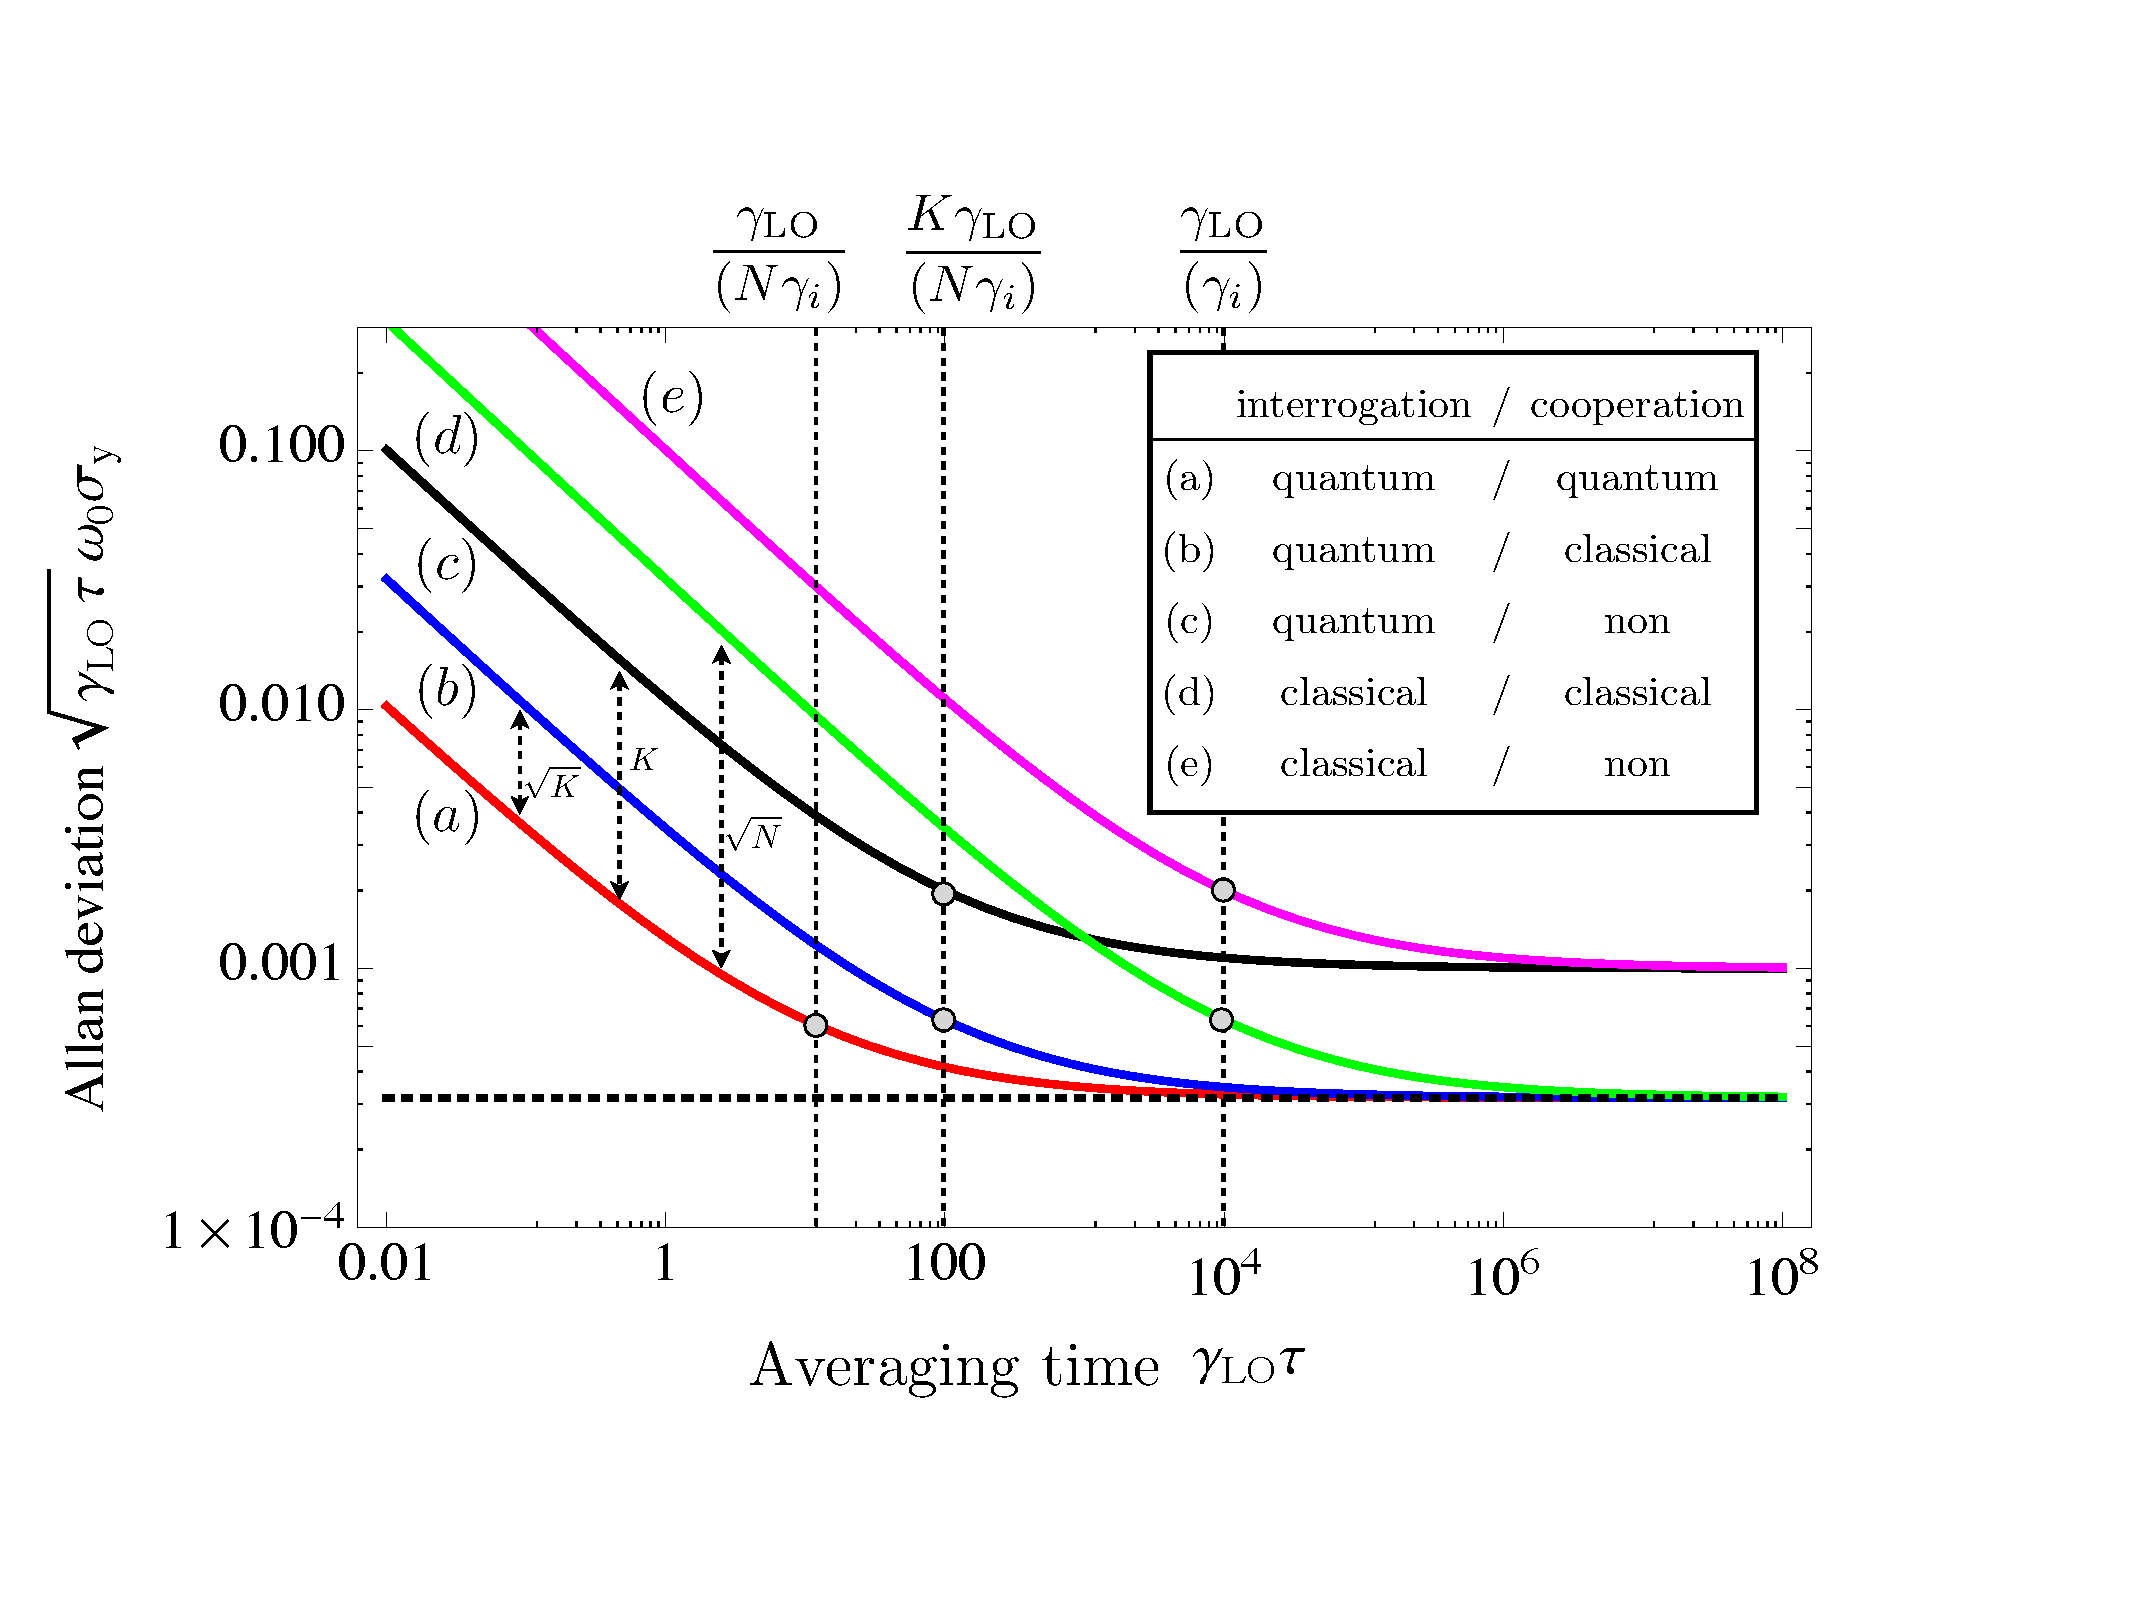
\includegraphics[width=1\textwidth]{./figs_Komar2014/fig3.pdf}
\caption
[Performance of different operation schemes]
{
\label{fig:comp}
Performance of different operation schemes. Comparison of
the achievable (rescaled) Allan deviation $\sqrt{\gamma_\mathrm{LO} \tau} \omega_0 \sigma_y$ using clock networks of different types and degrees of
cooperation. (a) the proposed protocol realizing quantum interrogation and
cooperation, (b) quantum interrogation and classical cooperation, (c) quantum
interrogation and no cooperation, (d) classical interrogation and classical
cooperation, (e) classical interrogation and no cooperation (cf. text). The
dotted base line represents the fundamental bound arising from the finite width
of the clock atoms transition
[compare \refeq{eq:ADEV2}]. This optimal stability can be attained only via cooperation between the
nodes.
The quantum clock network (a) represents the optimal form of cooperation, and reaches this boundary faster than any other
operational mode. Parameters are $N=1000$, $K=10$, $\gamma_i=10^{-4}\gamma_{LO}$.
 }
\end{figure}



Eventually, for large averaging times $\tau > 1/(\gamma_i N)$ the
Ramsey time becomes fundamentally limited by individual
noise processes that determine the atomic linewidth $T\leq 1/(\gamma_i N)$.
As a result, the $1/N$ scaling breaks down, and the ADEV returns to the square
root scaling with both the employed particle number and averaging time,
\begin{align}
\label{eq:ADEV2}
	\sigma_y(\tau) \sim \frac{ 1}{\omega_0 \sqrt N}
	\sqrt{\frac{\gamma_i}{\tau}},
\end{align}
up to constant numerical factors.  \refeq{eq:ADEV2} results from fundamental
quantum metrological bounds \cite{Escher:2011fn} (In the case of
dominating trap losses, the loss rate simply replaces $\gamma_i$ in the above
formula.), and represents the best conceivable clock stability in the presence
of individual particle decoherence which, in a network, can only be achieved via cooperation. Independently operating a clock, in contrast, can only achieve a stability scaling with the local number of atoms, i.e. $\sigma_y(\tau)\propto \sqrt{K/N}$.


 \reffig{fig:comp} illustrates the comparison of entangled clock network with
other approaches.
A network in which the $K$ nodes cooperate classically (curve b in
Fig.~\ref{fig:comp}), by locally measuring the individual phase deviation
$\phi_j$, and combining the outcomes via classical channels, outperforms
individually operated clocks (curve c) by a factor of $\sqrt K$ 
(for both cases, assuming optimal
quantum interrogation for individual nodes
\cite{Kessler2014,Borregaard2013_nearHeisenberg}).
The quantum network protocol (curve a)
increases this cooperative advantage by an additional factor of $\sqrt K$ for
short averaging times, reaching Heisenberg-limit, Furthermore the ADEV
converges to the fundamental bound [\refeq{eq:ADEV2}] $K$ times faster compared
to the case of classical cooperation (curve b).
Although an optimal, classical, local protocol
(e.g. \cite{Rosenband2013, Borregaard2013}), combined with classical
cooperation (curve d), eventually reaches the same
bound [\refeq{eq:ADEV2}],
% in this case, the obtainable stability is always
 % limited by the standard quantum limit with regard to the
% employed resources, $\sigma_y(\tau) \propto 1/\sqrt N$. Therefore,
this approach is atom-shot noise limited, and hence its stability is reduced by
a factor of  $\sqrt N$ for short averaging times [compare \refeq{eq:ADEV1}]
compared to the quantum network protocol.  Hence, the optimal stability
[\refeq{eq:ADEV2}] is reached at averaging times that are $N$ times longer
than for the proposed quantum network. Naturally, all of the above approaches
are superior to a classical scheme without cooperation (curve e).

As a specific example, we first consider ion clocks that can currently achieve a
stability of $2.8\times 10^{-15}$ after $1~\mathrm{s}$ of averaging time
\cite{Chou2010}. The entangled states of up to 14 ions has already been
demonstrated \cite{Monz2011} as was the entanglement of remote ions
\cite{Maunz2007}. We consider a network of ten clocks, each containing ten ions.
Using $\mathrm{Al}^+$ ($\omega_0 = 2\pi \times 1121~\mathrm{THz}$, $\gamma_i = 2\pi
\times 8~\mathrm{mHz}$), we find that the quantum cooperative protocol can reach
$4\times 10^{-17}$ fractional frequency uncertainty after $1~\mathrm{s}$. Larger
improvements could potentially be achieved using e.g. $\mathrm{Yb}^+$ ions, due to the long coherence time ($2.2\times
10^4~\mathrm{s}$) of its octupole clock transition.

The quantum gain could be even more pronounced for neutral atomic clocks. For a
network consisting of ten clocks similar to the one operated in JILA
\cite{Bloom2013}, each containing 1000 neutral atoms with central frequency
$\omega_0 = 2\pi\times 429~\mathrm{THz}$ and linewidth $\gamma_i = 2\pi \times
1~\mathrm{mHz}$,  the quantum cooperative scheme can achieve a stability of $\sim
2\times 10^{-18}$ after 1s averaging, and is an order of magnitude
better than the best classical cooperative scheme.  Future advances,
employing clock transitions with linewidths of a few tens of
$\mu\mathrm{Hz}$ (such as erbium), could possibly allow for further
improvement, achieving fractional frequency uncertainty beyond $10^{-20}$
after $\tau \sim 100~\mathrm{s}$. This level of stability is in the same order of
magnitude as the required sensitivity to successfully use the network as a
gravitational interferometer \cite{Schiller2008}.


So far we have assumed perfect operation and infinitely fast entanglement
distribution rates. In the SI we analyze these assumption and find that the
advantage of our scheme persists provided that fidelity  of the local collective
entangling \cite{MSgate} (which creates a GHZ state of $N/K$ qubits) exceeds the
threshold fidelity $F_\mathrm{th}$, where $1-F_\mathrm{th} \sim 1/(K\log N)$, and
the EPR sharing rate is higher than $R_\mathrm{EPR}\sim (\log N)^2 \gamma_i$.
For the optical clock example presented above, $F_\mathrm{th} \sim 0.99$, and
$R_\mathrm{EPR} \sim 1~\mathrm{Hz}$. While local operations with fidelity
$\sim 0.95$ have been realized for $N\sim 5$ ions \cite{Monz2011}, the errors
in such operations increase with $N$, making this realization more challenging.




\section{Security}
\label{sec:Security}
A network with such precise time-keeping capabilities can be subject to both internal
and external attacks. Effectively countering them is crucial to establish a
reliable ground for cooperation. We consider the network secure if the
implemented countermeasures can prevent external parties from benefiting from
the network (eavesdropping), as well as effectively detect any malicious activities of any of the members (sabotage).

Sabotage describes the situation where one of the nodes -- intended or
unintended -- operates in a damaging manner. For example, one node
% that is blatant enough to not comply with the formal requirements of the
% protocol is easily detected by the center within the time period of a single
% cycle, and then the particular node gets excluded from further cycles. More
% stealthy types of sabotage
could try sending false LO frequencies or wrong measurement bits in the hope of
corrupting the collective measurement outcomes. In order to detect such
malicious participants, the central node can occasionally perform assessment
tests of the different nodes by teleporting an uncorrelated qubit state
$[\ket{0} + e^{i\chi}\ket{1}]/\sqrt{2}$, where $\chi$ is a
 randomly chosen phase known only to the center. By checking for statistical
discrepancies between the measurement results and the detuning of the LO signal
sent by the node under scrutiny, the center can rapidly and reliably determine
whether the particular node is operating properly (See \reffig{fig:security}a
and Supplementary Information),
however this strategy breaks down, if multiple sabotage attacks
happen within a short time.
\begin{figure}
\centering
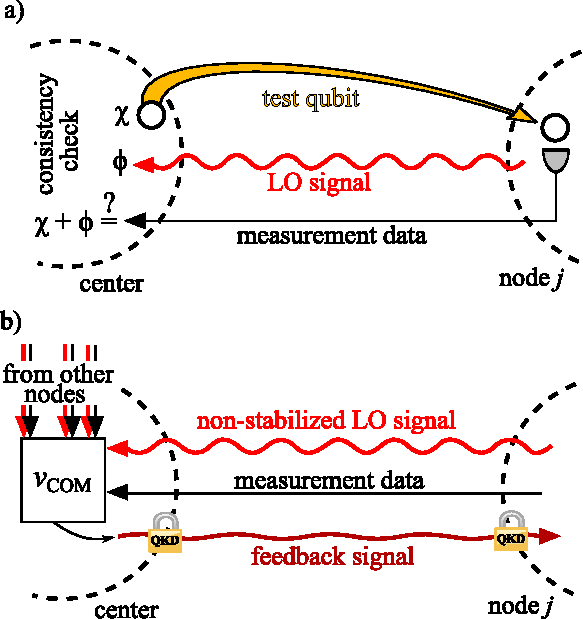
\includegraphics[width=0.7\textwidth]{./figs_Komar2014/fig4.pdf}
\caption
[Schematics of security countermeasures]
{
\label{fig:security}
Schematics of security countermeasures.
a) The center node can choose to test any node $j$ by teleporting a disentangled
qubit with a certain phase rotation. A properly operating node creates a local
GHZ state $[\ket{\mathbf{0}} + e^{i\chi}\ket{\mathbf{1}}]/\sqrt{2}$ from the
sent qubit,
 measures the parity of the GHZ state, and sends it to the center. The
measured parity holds information on the phase $\phi' = \chi + \phi$, where
$\phi$ is the accumulated phase of the LO at the node. The center verifies
$\phi$ by comparing it with the classically determined  phase of the sent LO
signal with respect to the COM signal.
b) Eavesdropping can be prevented by prescribing that only the non-stabilized LO
signals are sent through  classical channels and encoding the radio frequency
feedback signal with phase  modulation according to a shared secret key.
}
\end{figure}


Eavesdropping, i.e., the unauthorized attempt to access the stabilized
$\nu_\mathrm{COM}$ frequency, can be prevented by encoding the classical channels,
over which the center and the nodes exchange feedback signals, using quantum key
distribution protocols \cite{Gisin2002}. Our protocol can keep the stabilized
signal hidden from outsiders by mixing the feedback signal with the LO signal at each node only
after the non-stabilized LO has been sent to the center (see
\reffig{fig:security}b and SI). As a result, even if  all LO signals are intercepted, the eavesdropper is able to access
only the non-stabilized COM signal. Furthermore, the center exclusively can decode the
measurement results sent by the individual nodes using its own measurement outcomes as mentioned above. 
As a result, the stabilized COM signal remains
accessible exclusively to parties involved in the collaboration.

Finally, we note that a distributed operation offers significant security
advantages over an alternative approach of having all resources combined in one
place from where the signal is distributed. In case of a physical attack of the
network, disabling the center or the communication links, the nodes can fall
back to an independent clock operation using their local resources.

\section{Outlook}

One of the advantages of the proposed quantum clock network involves its ability
to maintain and synchronize the time standards across multiple parties in
real-time. 
% This can be achieved with classical cooperation schemes as well,
% however it arises naturally in the quantum scheme. 
Unlike the current world time standard, where the individual signals from
different clocks are averaged and communicated with a time delay (a so called
paper clock), in our quantum clock network all participants have access to the
ultra-stable signal at any time.
This makes it possible to measure systematic errors of different clocks in
real time, which in turn allows to correct them \cite{Bloom2013}, unlike in the
case of the paper clock which has to rely on the retrospectively averaged time 
signals (see SI). 
The enhanced stability of the network signal hereby allows for longer Ramsey
times in the control measurements used to determine the systematics of the
single clock.
% The longer Ramsey time allows this measurement to be carried
% out with precision limited only by the accuracy of the network.
Furthermore, by having full access to their local clocks the different parties
keep  their full sovereignty and ensure security, as opposed to a joint
operation of a single clock.

Realization of the full-scale network of the type described here will require a
number of technological advances in both metrology and experimental quantum
information science. 
% Practical realization can be based on optical atomic 
% clocks involving either trapped ions \cite{Chou2010} or neutral atoms
% \cite{Nicholson2012}.
% While ions provide a more straightforward implementation of the preparation of entangled qubit states \cite{Cirac2000, Monz2011}, state of the art neutral atom clocks
% feature large atom number resulting in better stability and potentially more
% significant quantum enhancement \cite{Nicholson2012}.
The remote entanglement can be implemented by using recently demonstrated
techniques for individual atom-photon entanglement \cite{Olmschenk2009,
Chou2007, togan, Bernien2013, Riste2013}. Since the teleportation protocol
requires quantum links capable of sharing EPR pairs with sufficiently high
repetition rate and fidelity, entanglement purification \cite{Dur1999} and
quantum repeater techniques \cite{duan3} will likely be required. In
practice, qubits used for entanglement distribution may not be ideal for clocks.
 However, as noted previously  remote entanglement does not need to involve
coherent qubits at optical frequencies (e.g., polarization entanglement can be
used). In such a case,   the use of hybrid approaches, combining  different
systems for entanglement and local clock operations, may be warranted.
Similarly, signals from clocks employing different transition frequencies
can be coherently connected by frequency combs, allowing clocks with different
clock qubits to participate.
% So far we have considered schemes requiring individual qubit addressing, however
It might also be interesting to explore if high-fidelity entangled EPR pairs can
be used to create remote entangled states of spin-squeezed type \cite{Leroux2010,
Sherson2006, Ma2012}, or by following the proposed approach for cat state
preparation in atomic ensembles \cite{McConnell2013}, 
or using collective interactions (such as \cite{MSgate}) and repetitive teleportation 
\cite{Andersen2013}.
% Alternatively, recently demonstrated  individual addressing in optical lattices
% \cite{Bakr2009, Lee2013} could be combined with entanglement swapping techniques
% to directly entangle optical lattice clocks.
% Lastly, the use of a continuous variable approach can be potentially explored to
% create squeezed atomic states across the network \cite{Sherson2006, Ma2012}. The
% use of collective measurements may allow one to reach Heisenberg limited
% stability \cite{Borregaard2013_nearHeisenberg}, while  squeezing can be transferred
% from photons to atomic ensembles \cite{Sherson2006, Hammerer2010}. An important
% open question of sensitivity of these techniques to photon losses needs to be
% addressed. 
In addition, while space-based communication networks will be capable
of maintaining optical phase coherence for the links between clocks, we note
that establishing ground-space coherent optical links remains a technical
challenge and requires an intense research effort which has recently started
\cite{Djerroud2010}.
% Beyond specific implementations, a number of other research directions may be
% explored. These include optimal eavesdropping, error correction and security
% strategies, robust feedback approaches minimizing technical imperfections such
% as Dick effect \cite{Santarelli1998}, as well as novel applications taking
% advantage of enhanced clocks with short averaging time.
Finally, if the entire network is spanned by satellites in space, the on-board
local oscillators can further benefit from the much lower noise level compared
to ground-based clocks.

If realized, such a quantum network of clocks can have important scientific,
technological, and social consequences. Besides creating a world platform for
time and frequency metrology, such a network may find important applications to
a range of technological advances for earth science \cite{Tapley2005},
precise navigation of autonomous vehicles and space probes (requiring high
 refresh rate), and to the test and search for the fundamental laws of
nature, including relativity and the connection between quantum and
gravitational physics \cite{Abramovici1992, Seidel2007, Schiller2008, Wolf2008}.
In order to explore these exciting applications one can either use the excellent
common frequency reference generated by the clock network, or, alternatively,
prepare modified collective states of different nodes that can directly measure
the specific signal under study. 
 







\chapter{Entangling collective Rydberg excitations of remote atomic ensembles}
\label{ch:Komar2015}
%%%%%%%%%%%%%%%%%%%%%%%%%%%%%%%%%%%%%%%%%%%%%%%%

\section{Introduction}
From \cite{}

\appendix 
\dsp 
\chapter{Appendices for Chapter \ref{ch:Komar2013}}
\label{app:Komar2013}

\section{Derivation of reflected mode operator}
\label{App: Reflection}

We obtain the reflected mode operator $c_R$ using input-output
relations for a two-sided cavity. 
By assuming that the two endmirrors have
the same transmittivity ($\propto\kappa$), we can write the input-output
relation for cavity mode $c_a$ on the driven mirror as
\bel
	c_{a,\text{out}} =
	\sqrt{\kappa}c_a - c_{a,\text{in}},
\eel
where $c_{a,\text{in}} = -i\frac{\Omega}{\sqrt{\kappa}}$ is the incoming field
operator on the mirror and $c_{a,\text{out}}$ is the output field operator.
For direct comparision with $c_a$ we
divide by $\sqrt{\kappa}$ and define the
reflection mode operator as  
$c_R \equiv c_{a,\text{out}}/\sqrt{\kappa} =
c_a +i\frac{\Omega}{\kappa}$.


\section{Analytic model}
\label{sect:App:steady_state}


%\label{sec:analytic_model}


In this appendix we provide the analytic solutions
used to calculate one- and two-time
correlation functions in steady state.
First, one-time correlations are calculated
from  the steady state solutions of
Eqs.~(\ref{eq:c000}--\ref{eq:c022}).
We set the time derivatives to zero and
solve the equations iteratively,
order by order in the weak drive.
This procedure yields
\bal
	\label{eq:alpha000}\bar A_{000} &\approx& 1,\\
	\label{eq:alpha100}\bar A_{100} &=& -i\alpha \frac{1}{1 + 4x^2},\\
	\label{eq:alpha011}\bar A_{011} &=& -\alpha \frac{2x}{1 + 4x^2},\\
	\label{eq:alpha200}\bar A_{200} &=& -\frac{\alpha^2}{\sqrt{2}}\frac{1 + 2x^2}{(1 +
	4x^2)(1 + 6x^2)},\\
	\label{eq:alpha111}\bar A_{111} &=& i\alpha^2\frac{2x}{(1 + 4x^2)(1 + 6x^2)},\\
	\label{eq:alpha022}\bar A_{022} &=& \alpha^2\frac{4x^2}{(1 + 4x^2)(1 + 6x^2)},
\eal
where $\alpha = \Omega/\tilde\kappa$ ($|\alpha|^2 \ll 1$), $x = g/(4\tilde\kappa)$ and
$\tilde \kappa = \kappa -i\Delta$.  
Using these amplitudes, we can express all
equal time averages.
The mean photon numbers are
\bal
	\bar n_a &=& |\bar A_{100}|^2 ,\\
	\bar n_s &=& |\bar A_{011}|^2 ,\\
	\bar n_R &=& \left|\bar A_{100} + i\frac{\Omega}{\kappa}\right|^2,
\eal 
and the photon-photon correlation functions are
\bal
\label{eq:g2aa0}
	g^{(2)}_{aa}(0) &=& \frac{2|\bar A_{200}|^2}{|\bar A_{100}|^4},\\
\label{eq:g2ss0}
	g^{(2)}_{ss}(0) &= & \frac{2|\bar A_{022}|^2}{|\bar A_{011}|^4},\\
\label{eq:g2AA0}
	g^{(2)}_{RR}(0) &= &
	\frac{\left|-\left(\frac{\Omega}{\kappa}\right)^2+
	2i\frac{\Omega}{\kappa}\bar A_{100} +
	\sqrt{2}\bar A_{200}\right|^2}
	{\left|i\frac{\Omega}{\kappa}+\bar A_{100}\right|^4}.
\eal
To
leading order in $\kappa/g$ these
yield Eqs.~(\ref{eq:na}--\ref{eq:g2AA}).


At finite temperature we calculate steady state amplitudes
within each phonon subspace $n$ similarly
in the ansatz of \refeq{eq:psi_thermal}.
Using the  notation $R_\kappa(\omega)$ introduced 
in Section \ref{sec:onetime_correlation},
the steady state amplitudes
within the subspace with $n$ phonons in the optical
groundstate are
\begin{align}
%p_{1,0,n}=
|\bar A_{10n}|^2=&\frac{\Omega^2\sqrt{R_\kappa(0)}}
{R_{\kappa}\left(\frac{g}{2}\sqrt{n+1}\right)},\\
|\bar A_{01n+1}|^2=&\frac{\Omega^2 g^2 (n+1) }{4
R_{\kappa}\left(\frac{g}{2}\sqrt{n+1}\right)},\\
|\bar A_{20n}|^2 =&\frac{ \Omega^4
R_\kappa(g/\sqrt{8})}{R_\kappa\left(g\sqrt{(2n+1)/8}\right)R_\kappa\left(\frac{g}{2}
\sqrt{n+1}\right)},\\
|\bar A_{02n+2}|^2 =&\frac{ \Omega^4 g^4 (n+1) (n+2)}{32
R_\kappa\left(g\sqrt{(2n+1)/8}\right)R_\kappa\left(\frac{g}{2}
\sqrt{n+1}\right)}.
\end{align}


Two-time correlation functions are calculated similarly,
using the conditional state after a jump
(see Eqs.~(\ref{eq:psi^a}) and (\ref{eq:psi^s}))
as the initial condition.
For example the
unnormalized state after detection of a photon in the
$c_a$ mode is $c_a\ket{\psi} =  \bar A_{100}\ket{000} +
	\sqrt{2}\bar A_{200}\ket{100} + \bar A_{111}\ket{011}$. 
We solve
Eqs.~(\ref{eq:c000}--\ref{eq:c011}) for the amplitudes 
with this state as initial
condition.
The finite delay correlation of the driven mode is
\bel
\begin{split}
	&g^{(2)}_{aa}(\tau) = \frac{|A_{100}(\tau)|^2}{|\bar A_{100}|^4}.
\end{split}
\eel
in good agreement with the numerics.
The correlation of the undriven
mode $g^{(2)}_{ss}(\tau)$ is calculated similarly. 
The unnormalized
state after detection in the $c_s$ mode is  $c_s\ket{\psi} = 
\bar A_{011}\ket{001}  + \bar A_{111}\ket{101} +  \sqrt{2}
\bar A_{022}\ket{012}$.
Using this  as the
initial
condition we solve Eqs.~(\ref{eq:c001}--\ref{eq:c012}) for the amplitudes
in the conditional state. 
In the limit of $\gamma \ll \kappa$ we obtain
\bel
	g^{(2)}_{ss}(\tau) 
	=
	\frac{|A_{012}(\tau)|^2}{|\bar A_{011}|^4}.
\eel 


\chapter{Appendices for Chapter \ref{ch:Stannigel2012}}
\label{app:Stannigel2012}


\section{Phonon nonlinearities}

In Eq. (8) in the main text we have derived an effective master equation (ME) to
describe the nonlinear interaction between two phonon modes. In the following we
present an alternative, more rigorous, approach, which illustrates the
individual approximations made in the derivation of the effective phonon
nonlinearity in more detail. We first consider only a single mechanical mode,
e.g. $b\equiv b_1$, which also allows us more easily to compare the results with
exact numerical calculations of the full model.


\subsection{Model}

We start with the full ME for the two optical modes coupled to a single
resonator mode, which in the frame of the driving frequency $\omega_L$ can be
written as
\begin{equation}\label{eq:SM_ME}
\dot \rho = -i[H_0+H_g+ H_\Omega(t),\rho] + \mathcal{L}_{\rm diss} \rho. \\
\end{equation}
Here 
\begin{equation}
H_0=  \omega_m b^\dag b - \Delta_s c_s^\dag c_s - \Delta_a  c_a^\dag c_a, 
\end{equation}
and
\begin{equation}
H_g= \frac{g_0}{2} \left(c_a c_s^\dag b^\dag +    c_a^\dag c_s  b \right),
\end{equation}
are the free evolution and the OM coupling, respectively,  $H_\Omega(t)=
i\Omega_s(t) (c_s^\dag - c_s)$ is the driving field for the symmetric mode with
slowly varying amplitude $\Omega_s(t)$ and
\begin{equation}
\mathcal{L}_{\rm diss} \rho  = \sum_{\eta=s,a} \kappa \mathcal{D}[c_\eta] \rho +
\frac{\gamma}{2} \mathcal{D}_{\rm th}[b]  \rho,
\end{equation}
accounts for dissipation. Here we have defined the superoperator
$\mathcal{D}_{\rm th}[b] = (N_{\rm th}+1)  \mathcal{D}[b] +  N_{\rm th} 
\mathcal{D}[b^\dag]$ to describe the coupling to a thermal bath.



\subsection{Displaced frame}

In contrast to the approach outlined in the main text, we now start our analysis
with a unitary displacement $U(t) c_sU^\dag (t)= c_s +\alpha(t)$ where the
classical cavity field $\alpha(t)$ obeys
\begin{equation}
\dot \alpha(t)= (i\Delta_s - \kappa) \alpha(t)  + \Omega_s(t). 
\end{equation}�
This unitary transformation eliminates the classical driving field and in the
new frame the resulting ME can be written as
\begin{equation}\label{eq:SM_FullME}
\begin{split}
\dot \rho = &-i[H_{\rm lin}+H_g,\rho] + \mathcal{L}_{\rm diss} \rho, \\
\end{split} 
\end{equation}
where $H_\Omega(t)$ has disappeared, but the linear part of the Hamiltonian now
contains an additional coupling between the resonator and the anti-symmetric
cavity mode,
\begin{equation}\label{eq:Hlin}
H_{\rm lin}�=  H_0  + G(t) c_a b^\dag + G^*(t) c_a^\dag b,
\end{equation} 
where $G(t)=g_0 \alpha(t)/2$. Note that ME \eqref{eq:SM_FullME} is still exact
and we will use this equation for our exact numerics below.


\subsection{Hybridized modes}

To proceed, we assume that $\alpha(t)$ is constant or slowly varying on the
timescale set by the detunings $|\Delta_a+\omega_m^i|$. This allows us to write
$H_{\rm lin}$ in its adiabatic eigenbasis
\begin{equation}
H_{\rm lin}�= - \Delta_s c_s^\dag c_s  - \tilde \Delta_a C^\dag C + \tilde
\omega_m B^\dag B,
\end{equation}
where  the $C$ and $B$ are bosonic operators for the hybridized mechanical and
optical modes and $\tilde \Delta_a$ and $\tilde \omega_m$ are the new
eigenfrequencies of $H_{\rm lin}$ for a given $G\equiv G(t)$.   We obtain
\begin{eqnarray}
C&=& \cos(\theta) c_a - \sin(\theta) b,\\
B&=& \cos(\theta) b + \sin(\theta) c_a,
\end{eqnarray}
where $\tan(2\theta)=-2|G|/\delta$ and
$\delta=-(\Delta_a+\omega_m)=2J-\omega_m-\Delta_s$. The shifted frequencies are
given by
\begin{eqnarray}
-\tilde \Delta_a&=& -\Delta_a - \frac{1}{2}\left( \delta - \sqrt{\delta^2+4|G|^2
}\right),\\
\tilde \omega_m &=& \omega_m - \frac{1}{2}\left( \delta +\sqrt{\delta^2+4|G|^2
}\right).
\end{eqnarray}
We see that by slowly increasing the classical control field $\alpha(t)$, the
mechanical mode $b$ is adiabatically converted into a polaronic mode $B$. For
small mixing angles $\theta$ the mode still retains its mechanical character,
while the finite photonic component is responsible for inducing an effective
nonlinearity.

In terms of the hybridized mode operators the dissipative terms can be written
as
\begin{equation}\label{eq:SM_Ldiss}
\begin{split}
\mathcal{L}_{\rm diss}\simeq& \kappa \mathcal{D}[c_s] + \kappa \cos^2(\theta)
\mathcal{D}[C] +   \frac{\gamma}{2}�\sin^2(\theta) \mathcal{D}_{\rm th}[C]  \\
+&  \frac{\gamma}{2}�\cos^2(\theta) \mathcal{D}_{\rm th}[B] + \kappa
\sin^2(\theta) \mathcal{D}[B]�.
\end{split} 
\end{equation}
In particular, we identify an additional optical decay channel with rate
$\gamma'=2 \kappa \sin^2(\theta)$ for the $B$ mode. In the following we define 
as
\begin{equation}
\tilde{\mathcal{L}}_\gamma =   \frac{\gamma}{2}�\cos^2(\theta)
\mathcal{D}_{\rm th}[B] + \frac{\gamma^\prime}{2} \mathcal{D}[B],
\end{equation}
the modified mechanical dissipation Liouvillian.
Note that in Eq.~\eqref{eq:SM_Ldiss} we have already neglected cross-terms
between $C$  and $B^\dag$. This is valid in the parameter regime considered
below, where $\kappa$ is small compared to the splitting of these two modes.
 

Finally, we also express the nonlinear interaction $H_g$ in terms of the
hybridized modes and write the result as
\begin{equation}\label{eq:SM_HgDecomp}
H_g= H_g^{(1)} + H_g^{(2)} + H_g^\prime. 
\end{equation}
Here, the first term is the one of interest 
\begin{equation}
H_g^{(1)} = \frac{g_0}{4}  \sin(2\theta)  \left( c_s + c_s^\dag\right) B^\dag B
,
\end{equation}
and describes the coupling of the $c_s$ mode to the number operator of the $B$
mode.
The second term is given by
\begin{equation}
H_g^{(2)} = -\frac{g_0}{2}  \sin^2(\theta)  \left( B  c_s^\dag C^\dag  + B^\dag 
c_s C \right),
\end{equation}
and leads to additional corrections. However, for small $\theta$ this term is
small compared to $H_g^{(1)}$. It can be further reduced if 
$|\Delta_s-\delta|\gg \Delta_s$.
Finally, the last term contains interactions
\begin{equation}
H_g^{\prime} = \frac{g_0}{2}  \cos^2(\theta)  \left( C c_s^\dag B^\dag  +
C^\dag  c_s B \right)  - \frac{g_0}{4}  \sin(2\theta)  \left( c_s +
c_s^\dag\right) C^\dag C,
\end{equation}
which can be neglected when either the $c_s$ or the $C$ mode are in the vacuum
state.


\subsection{Adiabatic elimination of the cavity mode}

Our goal is now to derive an effective ME for the mechanical degrees of freedom
only. To do so, we write the full ME as
\begin{equation}
\dot \rho = \left(\mathcal{L}_0 + \mathcal{L}_1\right)\rho,
\end{equation}
where 
\begin{equation}
\mathcal{L}_0\rho = -i[H_{\rm lin}+ H_g^\prime,\rho] + \mathcal{L}_{\rm diss}
\rho,
\end{equation}
and
\begin{equation}
\mathcal{L}_1\rho = -i[H_{g}^{(1)}+ H_g^{(2)},\rho].
\end{equation}
The dynamics of $\mathcal{L}_0$ does not excite the cavity modes, and therefore,
in the limit where $\tilde g=g_0\sin(2\theta)/4\rightarrow 0$ (either $g_0$ is
small or the mixing angle $\theta$ is small) the density operator can to a good
approximation be written as $\rho(t)=\rho_m(t) \otimes \rho_c^0$, where
$\rho_c^0$ is the vacuum state of the $c_s$ and the $C$ mode. To account for the
effects of a small $\mathcal{L}_1\sim\tilde g$ up to second order in
perturbation theory we define a projection operator onto this subspace,
\begin{equation}
\mathcal{P}\rho = {\rm Tr}_c\{ \rho \}\otimes \rho_c^0,
\end{equation}
and its complement $\mathcal{Q}=\mathds{1}-\mathcal{P}$. Then
\begin{eqnarray}
\mathcal{P}\dot \rho&=& \mathcal{P}\mathcal{L}_0\mathcal{P} \rho + \mathcal{P}
\mathcal{L}_{1}\mathcal{Q}\rho,\\
\mathcal{Q}\dot \rho&=& \mathcal{Q}(\mathcal{L}_0+\mathcal{L}_{1})\mathcal{Q}
\rho +  \mathcal{Q}\mathcal{L}_{1}\mathcal{P}\rho.
\end{eqnarray}
 Up to second order in $\tilde g$ we can formally integrate the equation for
 $\mathcal{Q}\rho$ and obtain
\begin{equation}
\mathcal{P}\dot{\rho}(t)\simeq\mathcal{P}\mathcal{L}_{0}\mathcal{P}\rho(t)+\mathcal{P}\mathcal{L}_{1}\int_{0}^{\infty}
 d\tau\, \mathcal{Q}
e^{\mathcal{L}_{0}\tau}\mathcal{Q}\mathcal{L}_{1}\mathcal{P}\rho(t).
\end{equation}
We define by $\rho_m(t)={\rm Tr}_c\{\mathcal{P} \rho(t)\}$ the reduced density
operator of the mechanical mode and write the final result as
\begin{equation}\label{eq:SM_Lm}
\dot\rho_m(t)=\left( \mathcal{L}^{(0)}_m+  \mathcal{L}^{(1)}_m   + 
\mathcal{L}^{(2)}_m\right) \rho_m(t).
\end{equation}
The first term describes the linear part of the dynamics  
\begin{equation}
\mathcal{L}^{(0)}_m \rho_m=  -i[ \tilde \omega_m B^\dag B,\rho_m] + 
\tilde{\mathcal{L}}_\gamma \rho_m,
\end{equation} 
with a modified frequency and modified decay rates for the $B$ mode. The other
two terms are given by
\begin{equation}\label{eq:SM_Lm1}
\mathcal{L}^{(1)}_m \rho_m = - \int_{0}^{\infty}  d\tau\, {\rm Tr}_c\{
[H_{g}^{(1)} , e^{\mathcal{L}_{0}\tau}\left([H_{g}^{(1)},\rho_m \otimes 
\rho_c^0] \right) ]\},
\end{equation}
and
\begin{equation}\label{eq:SM_Lm2}
\mathcal{L}^{(2)}_m \rho_m = - \int_{0}^{\infty}  d\tau\, {\rm Tr}_c\{
[H_{g}^{(2)} , e^{\mathcal{L}_{0}\tau}\left([H_{g}^{(2)},\rho_m \otimes 
\rho_c^0] \right) ]\}.
\end{equation}
 

\subsection{Simple perturbation theory}

In deriving Eq.~\eqref{eq:SM_Lm} we have so far only assumed that $\tilde g$ is
small compared to the typical frequency scales of the dynamics of the  $c_s$
mode. For now we will also assume that $g_0$ is small compared to $\delta$
\emph{and} $\Delta_s$. This allows us to neglect the term $H_g^\prime$ in
$\mathcal{L}_0$ and the cavity correlation functions in Eqs.~\eqref{eq:SM_Lm1}
and \eqref{eq:SM_Lm2} can be evaluated in a straight forward manner.  For the
action of $\mathcal{L}^{(1)}_m$ we obtain
\begin{equation}
\mathcal{L}^{(1)}_m \rho_m = -i  [\Lambda (B^\dag B)^2,\rho_m] + \Gamma_\phi
\mathcal{D} [B^\dag B],
\end{equation}
where $\Lambda=  {\rm Im} \{ S^{(1)}_{gg}(0) \}$,  $\Gamma_\phi=  {\rm Re}\{
S^{(1)}_{gg}(0)\}$   and
\begin{equation}
S^{(1)}_{gg} (\omega) = \tilde g^2\int_{0}^{\infty}  d\tau\, {\rm Tr}_c\{  c_s
e^{\mathcal{L}_{0}\tau} \left(c_s^\dag \rho_c^0\right)\}�e^{-i\omega \tau} .
\end{equation} 
We find $ S^{(1)}_{gg}(\omega)= \tilde g^2/(-i(\Delta_s+\omega) + \kappa)$ and
after inserting back the definition of $\tilde g$ in the limit
$|g_0\alpha/\delta| \ll 1$  we recover the expressions for $\Lambda$ and
$\Gamma_\phi$ given in Eq. (9) in the main text.
Similarly we obtain
\begin{equation}
\mathcal{L}^{(2)}_m \rho_m = -i  [ \delta \omega_m^{(2)}  B^\dag B,\rho_m] +
\frac{\gamma^{(2)}}{2} \mathcal{D} [B],
\end{equation}
where  $\delta \omega_m^{(2)}={\rm Im} \{ S^{(2)}_{gg}(\tilde \omega_m) \}$,
$\gamma^{(2)}=  {\rm Re}\{ S^{(2)}_{gg}(\tilde \omega_m)\}$   and
\begin{equation}
S^{(2)}_{gg} (\omega) = \frac{g_0^2 \sin^4(\theta)}{4}  \int_{0}^{\infty} 
d\tau\, {\rm Tr}_c\{  c_s C e^{\mathcal{L}_{0}\tau} \left(c_s^\dag C^\dag
\rho_c^0\right)\} e^{-i\omega \tau}.
\end{equation} 
The small frequency shift $\delta \omega_m^{(2)}$ can be absorbed into the
definition of $\tilde \omega_m$ and, since $\gamma^{(2)}\approx \gamma^\prime
\sin^2(\theta) g_0^2/(4\delta^2)$, for not too large mixing angles $\theta$,
$\gamma^{(2)}$ can always be neglected compared to $\gamma^\prime$. All together
the final effective phonon master equation is
\begin{equation}\label{eq:SM_EffectiveME}
\begin{split}
\dot \rho_m =& -i[\tilde \omega_m B^\dag B + \Lambda ( B^\dag B)^2 �, \rho_m ]
 + \Gamma_\phi \mathcal{D}[B^\dag B]\rho_m \\
&  + \frac{\gamma}{2}\mathcal{D}_{\rm th}[B] \rho_m  +  \frac{\gamma^\prime}{2} 
 \mathcal{D}[B]\rho_m,
\end{split} 
\end{equation}
which is the single resonator version of ME (8) given in the main text. 


\subsection{Corrections}

Let us now extend the above result to the case where $\tilde g$ is small
compared to $\Delta_s$ and $\delta$, but the bare interaction $g_0$ is not. In
this case the general expressions in Eqs.~\eqref{eq:SM_Lm1} and
\eqref{eq:SM_Lm2} still apply, but the effect of $H_g^\prime$ must be taking
into account when evaluating the correlation functions. To illustrate this, let
us assume that $g_0$ is still small compared to $\delta$. Then, by assuming that
the $C$ mode is initially in the ground state,  we obtain  approximately
\begin{equation}
H_{\rm lin} +H_g^\prime \approx - (\Delta_s- \Delta_B B^\dag B) c_s^\dag c_s,  
\end{equation}
where  the off-resonant frequency shift is 
\begin{equation}
\Delta_B= \frac{g_0^2\cos^4(\theta)}{4(\tilde \Delta_a+\tilde\omega_m
-\Delta_s))},
\end{equation}
and  can be comparable to $\Delta_s$. Therefore, we must evaluate the
correlation function for each phonon number state $|n\rangle$ separately and
write the resulting non-linear interaction as
\begin{equation}\label{eq:SM_EffectiveME_corr}
\mathcal{L}^{(1)}_m \rho_m = \sum_n n^2\left( -i  \left[\Lambda(n)
|n\rangle\langle n|�,\rho_m\right] + \Gamma_\phi(n)  \mathcal{D}
[|n\rangle\langle n| ])\right).
\end{equation}
Here $\Lambda(n)$ and $\Gamma_\phi(n)$   are the imaginary and real part of 
\begin{equation}
 S^{(1)}_{gg}(\omega=-n \Delta_B) =\frac{ n^2 \tilde g^2}{-i(\Delta_s-n\Delta_B)
 + \kappa}.
\end{equation}
We see that in this parameter regime more complicated nonlinearities can occur,
but the overall magnitude and the ratio between coherent and dephasing
interactions remains the same. In principle, this analysis can be extended to
the regime, where $g_0$ is comparable to $\delta$. However, in this case no
simple analytic expressions for $\lambda(n)$ and $\Gamma_\phi(n)$ can be derived
and need to be evaluated numerically.


\subsection{Numerical simulation} 

\begin{figure}
\centering
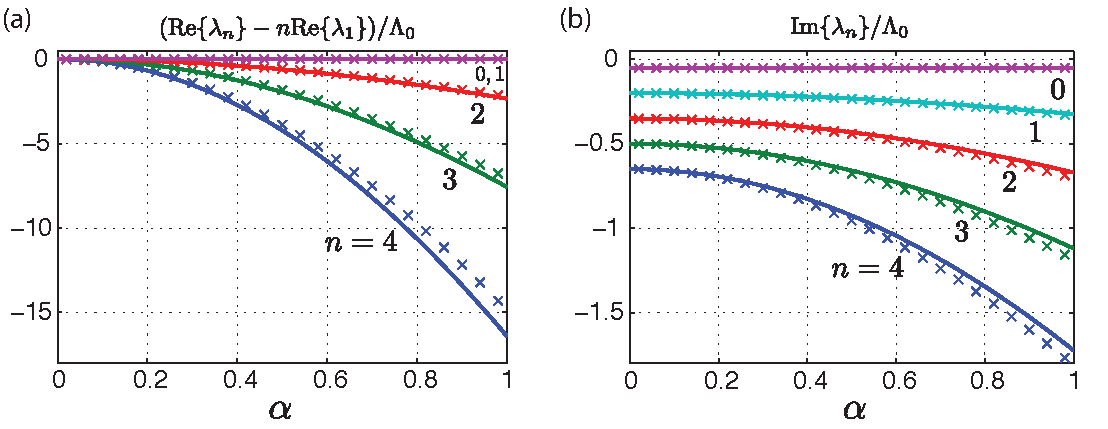
\includegraphics[width=1\textwidth]{./figs_Stannigel2012/Figure_suppl.pdf}
\caption
[Comparison of effective and exact description]
{Comparison of the effective analytic description
(Eqs.\,\eqref{eq:analytics}, lines) with exact eigenvalues of the Hamiltonian in
Eq.\,\eqref{eq:Hfull} (crosses) for different cavity field amplitudes $\alpha$.
All results are normalized to the scale
$\Lambda_0=g_0^4/(16\abs{\Delta_s}\delta^2)$ of the non-linearity.
(a) Deviation of the real parts of the eigenvalues from the result expected for
a linear oscillator, such that the splitting of the curves indicates an
effective non-linearity.
(b) Imaginary parts of the eigenvalues corresponding to decays. In both plots we
used the parameters $\Delta_s/g_0=-1$, $\delta/g_0=5$, $\kappa/g_0=2.5\times
10^{-2}$, $\gamma_m/g_0=2.5\times 10^{-4}$ and $N_{\rm th}=1$.}
\label{fig:numerics}
\end{figure}


To assess the validity of the effective phonon ME we now compare our result with
the dynamics of the full OMS.  Since we are mainly interested in the relation
between the phonon non-linearity and the corresponding dephasing and decay
rates, it is sufficient to evaluate the spectrum of the non-Hermitian
Hamiltonian, which  for the full model it is given by
\begin{equation}
\label{eq:Hfull}
\tilde H_{\rm full}=  H_{\rm lin}+ H_g - i\kappa c_s^\dag c_s - i\kappa
c_a^\dag c_a
 -i\frac{\gamma}{2} (N_{\rm th}+1) b^\dag b  -i\frac{\gamma}{2} N_{\rm th} b
b^\dag.
\end{equation}
In Fig.~\ref{fig:numerics} we plot the real and imaginary parts of the lowest
eigenvalues $\lambda_n$ of $\tilde H_{\rm full}$, which correspond to the lowest
number states $|n\rangle$ of the $B$ mode.
From the effective phonon model given in Eq.~\eqref{eq:SM_EffectiveME} and
\eqref{eq:SM_EffectiveME_corr} we obtain the approximate analytic results
\begin{subequations}
\label{eq:analytics}
\begin{equation}
{\rm Re} \{ \lambda_n\}= n \tilde \omega_m + n^2 \Lambda(n),
\end{equation}  
and
\begin{equation}
|{\rm Im} \{ \lambda_n\}|=\frac{\gamma}{2} N_{\rm th} + n \left(
\frac{\gamma}{2} (2N_{\rm th}+1) +\frac{\gamma^\prime}{2}\right) +n^2
\Gamma_\phi(n).
\end{equation}
\end{subequations}
We see a good agreement between these results for the effective model and the
exact numerics, both for the real and imaginary parts. Although there are some
deviations due to higher-order effects, the effective non-linear splitting
(Fig.~\ref{fig:numerics}(a)) is much larger than the induced decoherence
(Fig.~\ref{fig:numerics}(b)), as is expected for the chosen parameters. Hence,
we conclude that the effective model accurately describes the dynamics of the
mechanical resonator, and that the effective phonon non-linearity may serve as a
basis for gate operations as discussed in the main text and in the following
section.


\section{Phonon-phonon interactions} 

The derivation of the effective phonon nonlinearity, as outlined above for a
single resonator, can be easily adapted to two resonators as discussed in the
main text.
In this case we have 
\begin{equation}
H_0=  \sum_{i=1,2} \omega^i_m b_i^\dag b_i - \Delta_s c_s^\dag c_s - \Delta_a 
c_a^\dag c_a,
\end{equation}
and
\begin{equation}
H_g= \frac{g_0}{2} \left[c_a c_s^\dag (b^\dag_1-b_2^\dag) +    c_a^\dag c_s 
(b_1-b_2)\right].
\end{equation}
After changing into the displaced representation to eliminate the driving field
we obtain the linearized Hamiltonian
\begin{equation}
H_{\rm lin}�=  H_0  + \sqrt{2}\left( G(t)  c_a b_a^\dag + G^*(t) c_a^\dag
b_a\right),
\end{equation} 
where $b_a=(b_1-b_2)/\sqrt{2}$ and $G(t)=g_0\alpha(t)/2$.
For similar mechanical frequencies $\omega_m^1\simeq \omega_m^2=\omega_m$ the
symmetric resonator mode is decoupled and we can simply repeat the analysis from
above by identifying $b\equiv b_a$ and replacing $g_0$ by $\sqrt{2}g_0$.

For arbitrary $\omega_i$, we write the linear part of the Hamiltonian in its
diagonal form
\begin{equation}\label{eq:Hlin2}
H_{\rm lin}�=  - \Delta_s c_s^\dag c_s -  \tilde \Delta_a  C^\dag C + \tilde
\omega_1 B_1^\dag B_1 + \tilde \omega_2 B_2^\dag B_2.
\end{equation} 
As in the single-resonator case the $c_s$ mode is unaffected,  but the $c_a$
mode now couples to both $b_1$ and $b_2$.  The resulting hybridized modes $C$,
$B_\pm$ depend on the choice of parameters $\omega_m^{1,2}, \Delta_a$ and $G$.
For the case of interest, i.e. for a symmetric detuning
$\omega_m^{1,2}=-\Delta_a \mp \delta$, we obtain
\begin{eqnarray}
C&=& \cos(2\Theta) c_a -  \sin(2\Theta)(B_1 + B_2)/\sqrt{2},\\
B_1&=& \cos^2(\Theta) b_1 + \sin(2\Theta) c_a/\sqrt{2} -  \sin^2(\Theta)b_2,\\
B_2&=& \cos^2(\Theta) b_2 + \sin(2\Theta) c_a/\sqrt{2} -  \sin^2(\Theta)b_1,
\end{eqnarray} 
where $\tan(2\Theta)=-\sqrt{2} |G|/\delta$. Therefore, for small $\Theta$ the
modes $B_{1,2}$ correspond to the original mechanical resonator modes $b_{1,2}$
and $\tilde \omega_i\approx \omega_m^{i}$.

As above, we can now re-express the dissipation and the non-linear coupling
$H_g$ in terms of $C$ and $B_\pm$. The modified mechanical dissipation terms are
given
\begin{equation}
\tilde{\mathcal{L}}_\gamma =  \sum_{i=1,2}  \frac{\gamma}{2}�\cos^2(2\Theta)
\mathcal{D}_{\rm th}[B_i] + \frac{\kappa}{2} \sin^2(2\Theta) \mathcal{D}[B_i],
\end{equation}
and for small $\Theta$ the optical decay rate $\gamma^\prime =\kappa
\sin^2(2\Theta)$ is the same as given above and in the main text.
Using the decomposition of the non-linear coupling as done in
Eq.~\eqref{eq:SM_HgDecomp},  we obtain
\begin{equation}
H_g^{(1)}= \frac{g_0}{\sqrt{8} }\sin(2\Theta)   \left( c_s+c_s^\dag\right)
\left(B_1^\dag B_1 - B^\dag_2 B_2\right),
\end{equation} 
the contribution $H_g^{(2)}$ vanishes and 
\begin{equation}
H_g^{\prime}= \frac{g_0}{2  }\cos(2\Theta)   \left( C c_s^\dag
(B_1^\dag-B_2^\dag) + {\rm H.c.}  \right).
\end{equation}
We see that the structure and also the relative frequency scales are identical
to the corresponding terms discussed for the single resonator above. Therefore,
under the same conditions we can eliminate the cavity mode and  obtain the
effective phonon master equation
\begin{equation}
\begin{split}
\dot \rho_m =& -i\left[\sum_i \tilde \omega_i B_i^\dag B_i + \Lambda (B_1^\dag
B_1-B_2^\dag B_2)^2 �, \rho_m \right]  \\
&+ \Gamma_\phi \mathcal{D}[(B_1^\dag B_1-B_2^\dag B_2)]\rho_m   +
\tilde{\mathcal{L}}_\gamma \rho_m.
\end{split} 
\end{equation}
 For small $\Theta$ this equation reduces to ME  (8) in the main text and
 higher-order corrections can be included in the same way as discussed for the
 single resonator case.

\chapter{Appendices for Chapter \ref{ch:Borregaard_PRL2015}}
\label{app:Borregaard_PRL2015}

This appendix describes the details of the
perturbation theory and the derivation of the effective Hamiltonian
$\hat{H}_{\text{eff}}$ and effective Lindblad operators. We describe the
situation both with and without a two-photon drive. Furthermore, we present the
results of a numerical simulation of the full dynamics of the gates to verify
the results found with perturbation theory and address the question of how
strong a drive we can allow for. In the end, this determines the gate time as
described in the article. Finally we discuss of the additional errors described
in the final part of the article.

\section{Perturbation theory}

We will now give the details of the perturbation theory and the derivation of
the effective operators together with the success probabilitites, gate times and
gate errors (see \tabref{tab:table1}). Our perturbation theory is based on the
effective operator formalism described in Ref.~\cite{Florentin}.
 
\begin{table} [h]
\centering
\begin{tabular}{|c|c|c|c|c|}
\hline
Gate & Origin of error & Error & Probability & Time  \\ \hline CZ-gate &
\specialcell{$\gamma_{g}=0$
\\$\gamma_{g}>0$} & \specialcell{$0$\\$\sim
\frac{\gamma_{g}}{\gamma\sqrt{C}}$} & $\sim 1-\frac{6}{\sqrt{C}}$ &
$\sim\frac{15\pi\sqrt{C}\gamma}{2\Omega^{2}}$\\ \hline Toffoli &
\specialcell{$\Gamma_{i}\neq\Gamma_{j}$\\$\gamma_{g}>0$} &
\specialcell{$\lesssim\!\frac{0.3}{C}\quad$\\$\sim\!\!
\frac{\gamma_{g}}{\gamma\sqrt{C}}$} & $\sim 1-\frac{3}{\sqrt{C}}$ &
$\sim\frac{4\pi\sqrt{C}\gamma}{\Omega^{2}}$ \\ \hline
\end{tabular}
\caption
[Comparison of CZ and Toffoli gates]
{The errors, success probabilities and gate times of the $N$-qubit
Toffoli gate and the $CZ$-gate considered in the article. Note that the
branching fraction $\gamma_{g}/\gamma$ can be made arbitrarily small using a far
detuned two-photon driving as explained in below. $\Gamma_{i}$ is the rate of
detectable errors for the qubit state with $i$ qubits in state $\ket{1}$. The
success probability of the CZ-gate can be increased at the expense of an error
scaling of $1/C$ as explained in the article.}
\label{tab:table1}
\end{table}  

First, we treat the simplest situation where the auxiliary atom is directly
driven to an excited state $\ket{E}$ by a weak classical drive $\Omega$ as shown
in \reffig{fig:figureS1} (reproduced from Fig. 1 in the article). Note that we
allow for some decay from $\ket{E}\to\ket{g}$ with decay rate $\gamma_{g}$ as
opposed to the situation in the article. We will later consider the situation
where this decay rate is suppressed using a two-photon drive. The level
structure of the qubit atoms are also shown in \reffig{fig:figureS1}.

\begin{figure} [H]
\centering
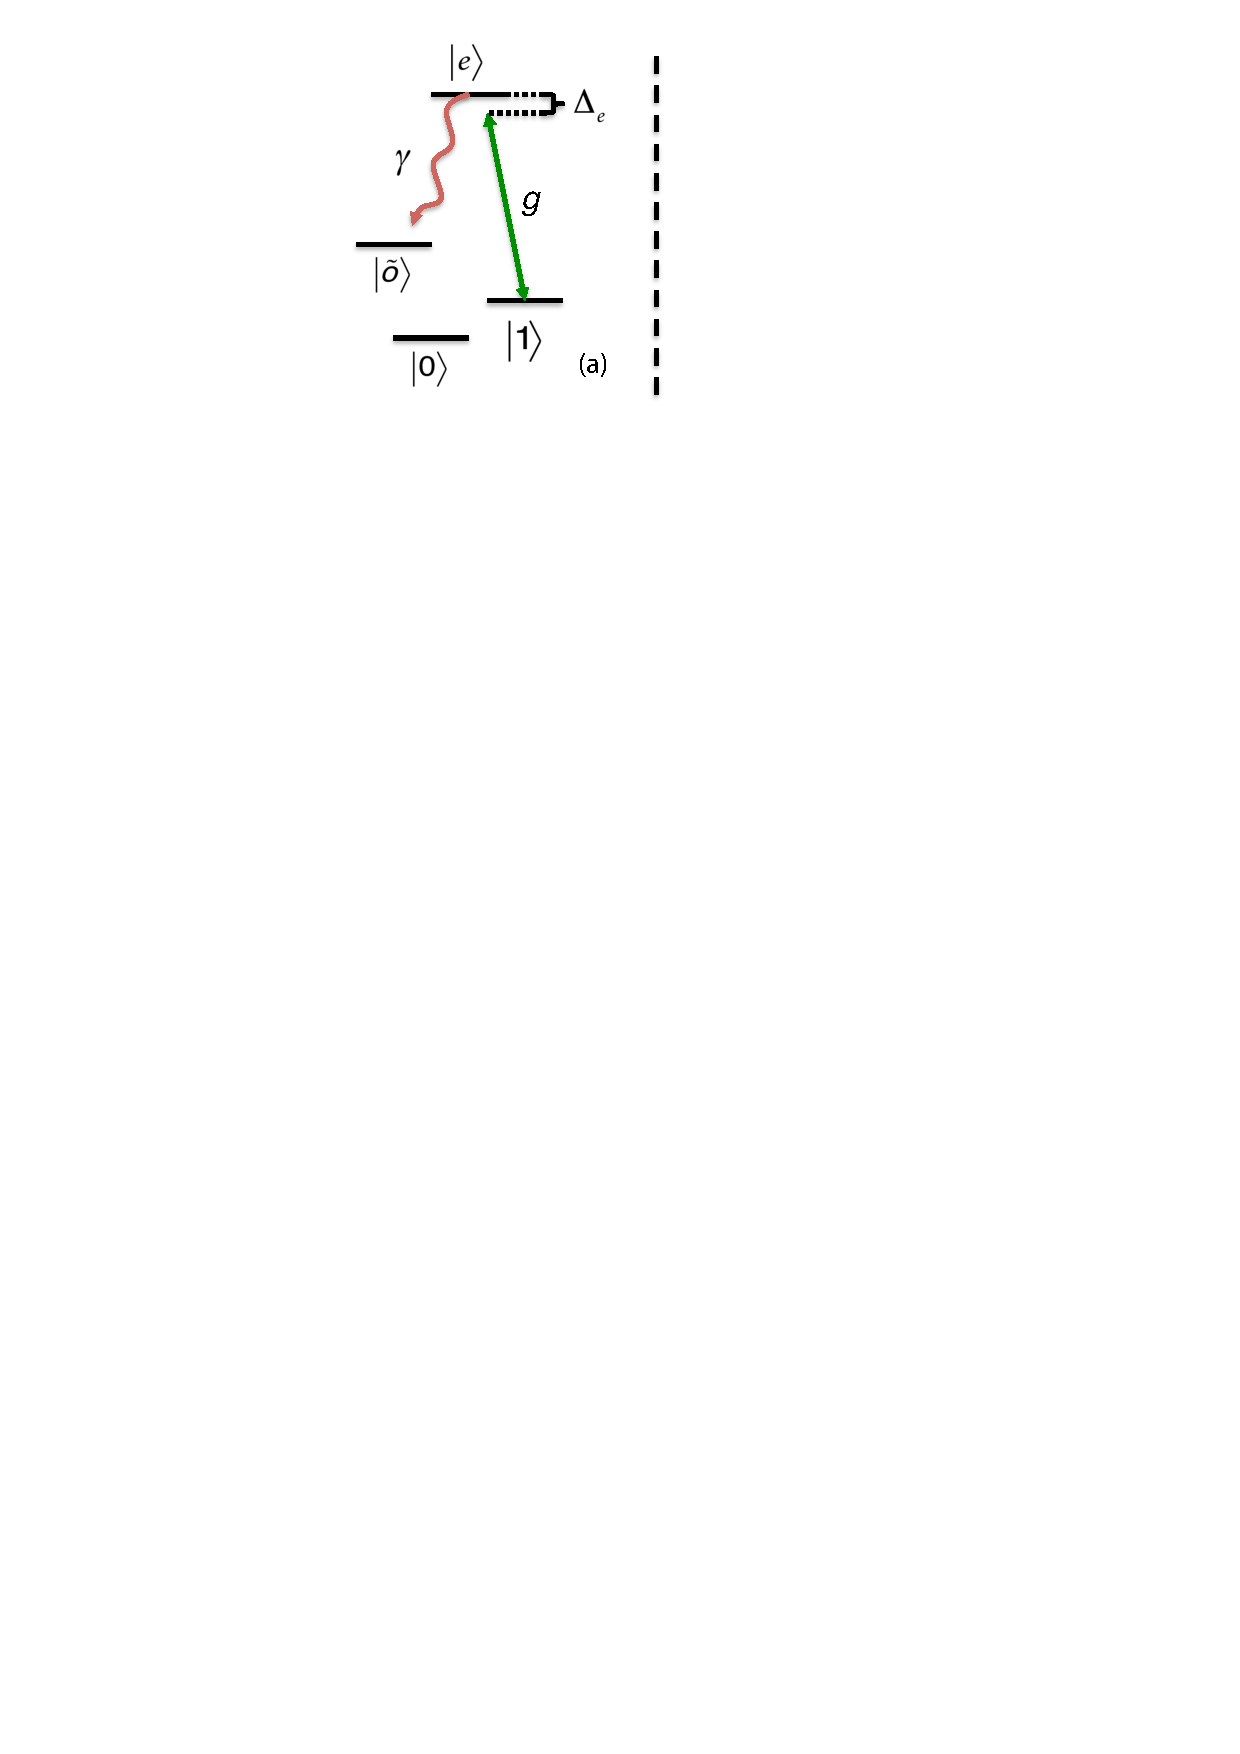
\includegraphics[width=0.35\textwidth]{./figs_Borregaard_PRL2015/figureS1a}
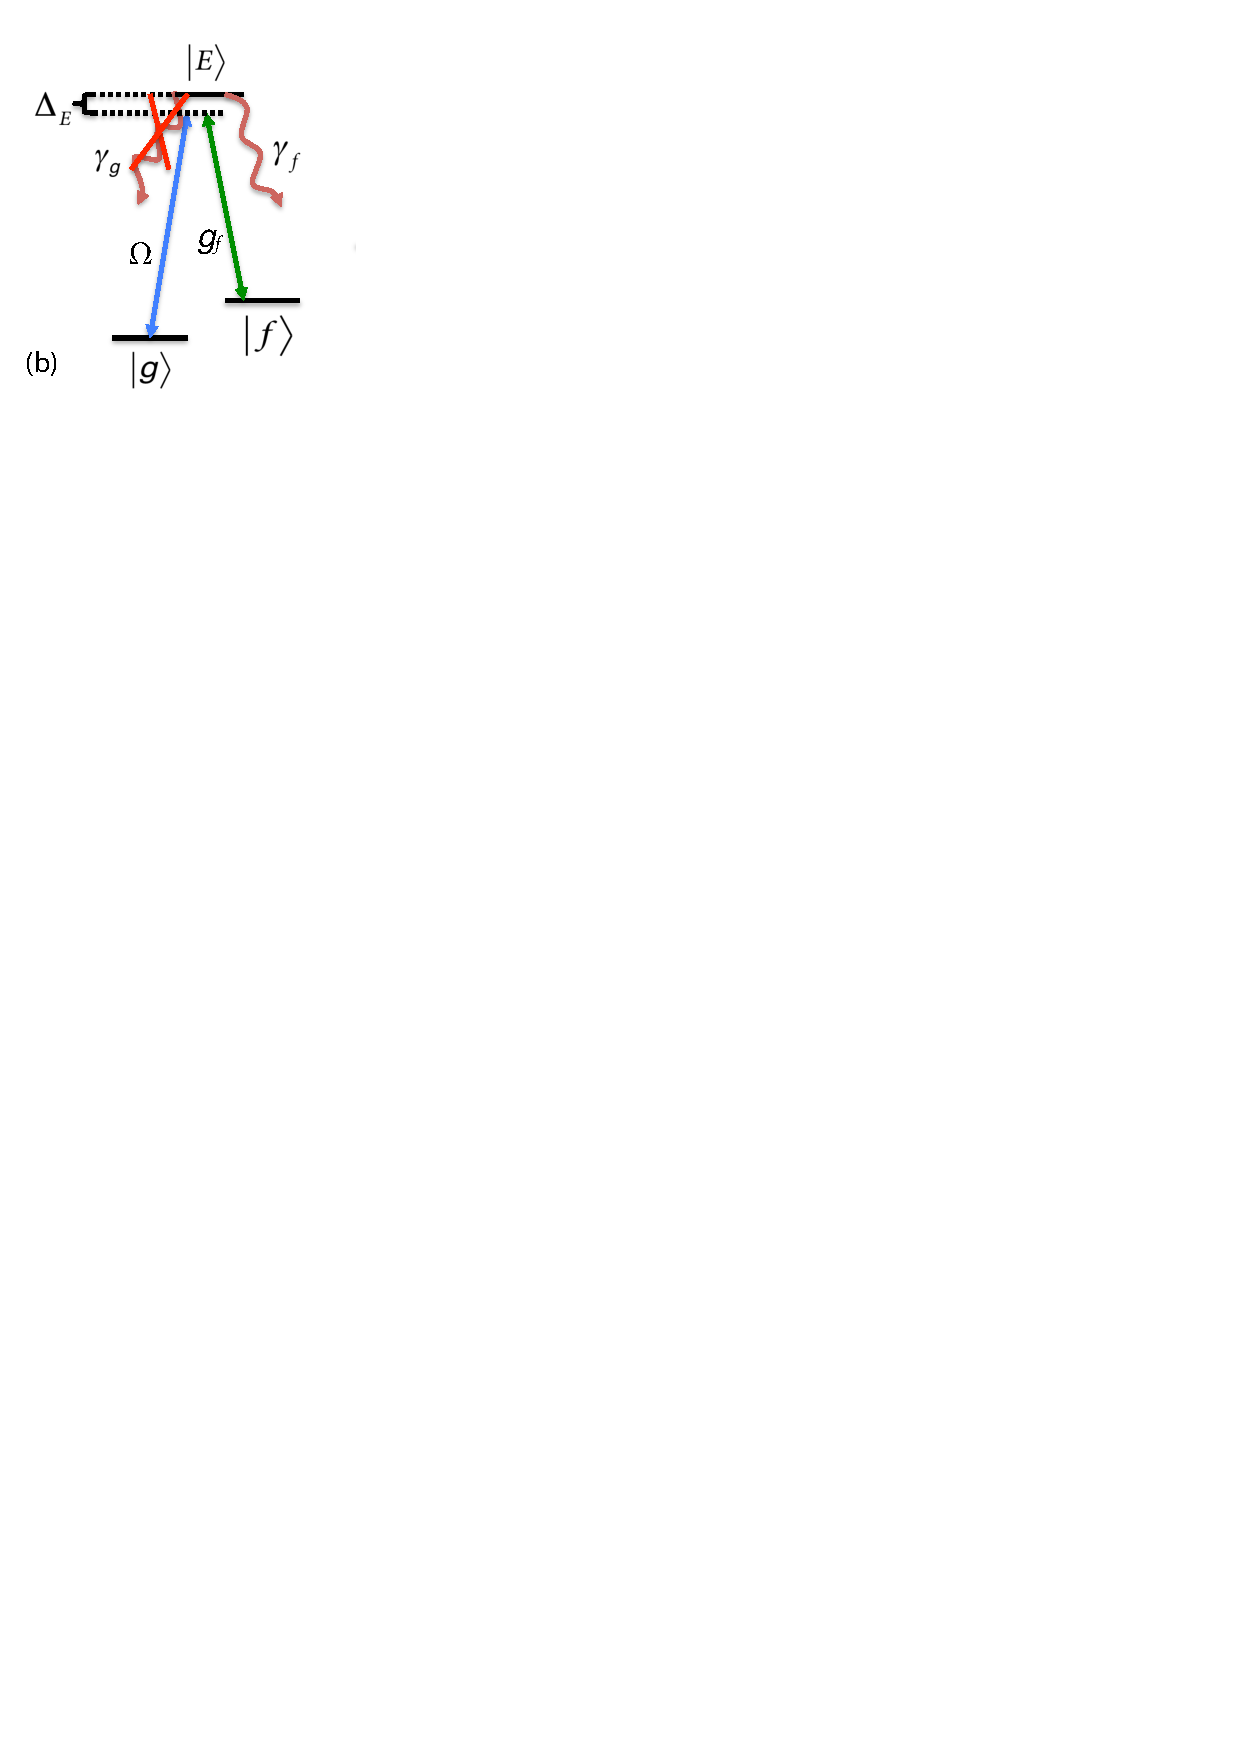
\includegraphics[width=0.35\textwidth]{./figs_Borregaard_PRL2015/figureS1b}
\caption
[Level structure of qubit an auxiliary atoms]
{(a) Level structure of the qubit atoms. Only state $\ket{1}$ couples
to the cavity and we assume that the excited level decays to some level
$\ket{\tilde{o}}$, possible identical to $\ket{f}$ or $\ket{0}$. (b) Level
structure of the auxiliary atom and the transitions driven by the weak laser
($\Omega$) and the cavity ($g_{f}$). We allow for some decay from
$\ket{E}\to\ket{g}$ with decay rate $\gamma_{g}$. }
\label{fig:figureS1}
\end{figure}

The Hamilton describing the system in a proper rotating frame is given by Eqs.
(1)-(3) in the article and is reproduced here
\begin{eqnarray} \label{eq:hamil1}
\hat{H}&=&\hat{H}_{e}+\hat{V}+\hat{V}^{\dagger}, \\
\hat{H}_{e}&=&\Delta_{E}\ket{E}\bra{E}+g_{f}(\hat{a}\ket{E}\bra{f}+H.c) \nonumber \\
&&+\sum_{k}\Delta_{e}\ket{e}_{k}\bra{e}+g(\hat{a}\ket{e}_{k}\bra{1}+H.c), \\
\hat{V}&=&\frac{\Omega}{2}\ket{E}\bra{g},
\end{eqnarray}          
where we have assumed for simplicty that all couplings ($g,\Omega$) are real and
$k$ labels the qubit atoms ($\hbar=1$). We have defined
$\Delta_{E}=\omega_{E}-\omega_{g}-\omega_{L}$, and
$\Delta_{e}=\omega_{e}-\omega_{g}-\omega_{L}+\omega_{f}-\omega_{1}$ where
$\omega_{L}$ is the laser frequency and otherwise $\omega_{x}$ is the frequency
associated with level $x$. Note that we assume the cavity frequency to be
$\omega_{c}=\omega_{L}+\omega_{g}-\omega_{f}$ such that we are on resonance with
the $\ket{g}\to\ket{E}\to\ket{f}$ two-photon transition.

The dissipation in the system is assumed to be described by Lindblad operators
such that $\hat{L}_{0}=\sqrt{\kappa}\hat{a}$ describes the cavity decay with
decay rate $\kappa$, $\hat{L}_{g}=\sqrt{\gamma_{g}}\ket{g}\bra{E}$, and
$\hat{L}_{f}=\sqrt{\gamma_{f}}\ket{f}\bra{E}$ describes the decay of the
auxiliary atom and $\hat{L}_{k}=\sqrt{\gamma}\ket{\tilde{o}}_{i}\bra{e}$
describes the decay of the qubit atoms ($k=1,2\ldots N$). As described in the
article $\ket{\tilde{o}}$ may or may not coincide with $\ket{0}$ or $\ket{1}$.
Assuming that $\Omega$ is weak ($\Omega^{2}/\Delta_{E}\ll\Delta_{E}$ and
$\Omega\ll g$), we can treat the driving as a perturbation to the system. As
shown in Ref.~\cite{Florentin}, the dynamics of the system is then governed by
an effective master equation of the form
\begin{equation}
\dot{\rho}=i\left[\rho,\hat{H}_{\text{eff}}\right] +
\sum_{x}\hat{L}_{x}^{\text{eff}}\rho(\hat{L}_{x}^{\text{eff}})^{\dagger}-\frac{1}{2}\left((\hat{L}_{x}^{\text{eff}})^{\dagger}\hat{L}_{x}^{\text{eff}}\rho+\rho(\hat{L}_{x}^{\text{eff}})^{\dagger}\hat{L}_{x}^{\text{eff}}\right),
\end{equation}
where $\rho$ is the density matrix of the system, $\hat{H}_{\text{eff}}$ is an
effective Hamiltonian, and  $L_{x}^{\text{eff}}$ are effective Lindblad
operators with $x=0,g,f,k$.  The effective operators are found from:
\begin{eqnarray} \label{eq:supheff1}
\hat{H}_{\text{eff}}&=&-\frac{1}{2}\hat{V}^{\dagger}\left(\hat{H}_{\text{NH}}^{-1}+(\hat{H}_{\text{NH}}^{-1})^{\dagger}\right)\hat{V}
\\
\hat{L}_{x}^{\text{eff}}&=&\hat{L}_{x}\hat{H}_{\text{NH}}^{-1}\hat{V},  \label{eq:supleff1}
\end{eqnarray}
where 
\begin{equation}
\hat{H}_{\text{NH}}=\hat{H}_{e}-\frac{i}{2}\sum_{x}\hat{L}_{x}^{\dagger}\hat{L}_{x},
\end{equation}
is the no-jump Hamiltonian. The Hilbert space of the effective operators can be
described in the basis of $\left\{\ket{g},\ket{f}\right\}$ of the auxiliary atom
and the states $\left\{\ket{0},\ket{1},\ket{\tilde{o}}\right\}$ of the qubit
atoms. To ease the notation, we define the projection operators $\hat{P}_{n}$
which projects on to the states with $n$ qubits in state $\ket{1}$. From
Eq.~\eqref{eq:supheff1} and \eqref{eq:supleff1} we then find:
\begin{eqnarray}
\hat{H}_{\text{eff}}&=&\sum_{n=0}^{N}\frac{-\Omega^{2}}{4\gamma}\mathrm{Re}\left\{\frac{i\tilde{\Delta}_{e}/2+nC}{\tilde{\Delta}_{e}(i\tilde{\Delta}_{E}/2+C_{f})+\tilde{\Delta}_{E}nC}\right\}\ket{g}\bra{g}\otimes \hat{P}_{n} \nonumber \\
&=&\sum_{n=0}^{N}\Delta_{n}\ket{g}\bra{g}\otimes \hat{P}_{n}
\label{eq:supham2}\\
\hat{L}_{0}^{\text{eff}}&=&\sum_{n=0}^{N}\frac{1}{2\sqrt{\gamma}}\frac{\sqrt{C_{f}}\tilde{\Delta}_{e}\Omega}{\tilde{\Delta}_{e}(i\tilde{\Delta}_{E}/2+C_{f})+n\tilde{\Delta}_{E}C}\ket{f}\bra{g}\otimes
\hat{P}_{n} \nonumber \\
&=&\sum_{n=0}^{N}r_{0,n}^{\text{eff}}\ket{f}\bra{g}\otimes \hat{P}_{n}
\label{eq:subleff1} \\
\hat{L}_{g}^{\text{eff}}&=&\sum_{n=0}^{N}\frac{1}{2}\frac{(i\tilde{\Delta}_{e}/2+nC)\Omega}{\tilde{\Delta}_{e}(i\tilde{\Delta}_{E}/2+C_{f})+n\tilde{\Delta}_{E}C}\frac{\sqrt{\gamma_{g}}}{\gamma}\ket{g}\bra{g}\otimes
\hat{P}_{n} \nonumber \\
&=&\sum_{n=0}^{N}r_{g,n}^{\text{eff}}\ket{g}\bra{g}\otimes \hat{P}_{n} \\
\hat{L}_{f}^{\text{eff}}&=&\sum_{n=0}^{N}\frac{1}{2}\frac{(i\tilde{\Delta}_{e}/2+nC)\Omega}{\tilde{\Delta}_{e}(i\tilde{\Delta}_{E}/2+C_{f})+n\tilde{\Delta}_{E}C}\frac{\sqrt{\gamma_{f}}}{\gamma}\ket{f}\bra{g}\otimes
\hat{P}_{n} \nonumber \\
&=&\sum_{n=0}^{N}r_{f,n}^{\text{eff}}\ket{f}\bra{g}\otimes \hat{P}_{n} \\
\hat{L}_{k}^{\text{eff}}&=&\sum_{n=1}^{N}-\frac{1}{2\sqrt{\gamma}}\frac{\sqrt{C_{f}}\sqrt{C}\Omega}{\tilde{\Delta}_{e}(i\tilde{\Delta}_{E}/2+C_{f})+n\tilde{\Delta}_{E}C}\ket{f}\bra{g}\otimes\ket{\tilde{o}}_{k}\bra{1}\otimes\hat{P}_{n}
\nonumber \\
&=&\sum_{n=1}^{N}r_{n}^{\text{eff}}\ket{f}\bra{g}\otimes\ket{\tilde{o}}_{k}\bra{1}\otimes\hat{P}_{n},
\label{eq:subleff2}
\end{eqnarray}
where we have defined the cooperativities $C_{(f)}=g_{(f)}^{2}/\gamma\kappa$ for
the qubit (auxiliary) atoms and the complex detunings
$\tilde{\Delta}_{E}\gamma=\Delta_{E}-i\gamma_{f}/2$ and 
$\tilde{\Delta}_{e}\gamma=\Delta_{e}-i\gamma/2$. Note that we have defined the
parameters $r^{\text{eff}}_{0,n}, r^{\text{eff}}_{g,n},r^{\text{eff}}_{f,n}$ and
$r_{n}^{\text{eff}}$ in Eqs. \eqref{eq:subleff1}-\eqref{eq:subleff2} to
characterize the decays described by the Lindblad operators. Note that
$r_{0}^{\text{eff}}=0$. In our calculations we parametrize the difference
between the auxiliary atom and the qubit atoms by $C_{f}=\alpha C$ and
$\gamma_{f}=\beta\gamma$ to easier treat the limit of $C\gg1$ that we are
interested in.

\subsection{Success probability and fidelity}
Eqs. \eqref{eq:subleff1}-\eqref{eq:subleff2} show that the effect of all
Lindblad operators, except $\hat{L}_{g}^{\text{eff}}$, is that the state of the
auxiliary atom is left in state $\ket{f}$. All these errors are thus detectable
by measuring the state of the auxiliary atom at the end of the gate. For the
heralded gates where we condition on measuring the auxiliary atom in state
$\ket{g}$ at the end of the gates, these detectable decays therefore do not
effect the fidelity of the gates but only the success probability.  The rate
$\Gamma_{n}$ of the detectable decays for a state with $n$ qubits in state
$\ket{1}$ is
$\Gamma_{n}=\abs{r_{0,n}^{\text{eff}}}^{2}+\abs{r_{f,n}^{\text{eff}}}^{2}+\abs{r_{n}^{\text{eff}}}^{2}$
and assuming an initial qubit state described by density matrix $\rho_{qubit}$
the success probability of the gates is
\begin{equation}
P_{\text{success}}=
\sum_{n=0}^{N}\text{Tr}
\left\{e^{-\Gamma_{n}t_{\text{gate}}}\rho_{\text{qubit}}\hat{P}_{n}\right\},
\end{equation}
where $t_{\text{gate}}$ is the gate time and $\text{Tr}$ denotes the trace. 

Having removed the detrimental effect of the detectable errors by heralding on a
measurement of the auxiliary atom the fidelity of the gates will be determined
by more subtle, undetectable errors (see below). We define the fidelity, $F$ of
the gate as
\begin{equation}
F=\frac{1}{P_{\text{success}}}\bra{\psi}\bra{g}
\tilde{\rho}_{\text{qubit}}\ket{g}\ket{\psi},
\end{equation} 
where we have assumed that the ideal qubit state after the gate is a pure state
$\ket{\psi}$ and $\tilde{\rho}_{qubit}$ is the actual density matrix of the
qubits and the auxiliary atom after the gate operation.

\subsection{$N$-qubit Toffoli gate}

As shown in the article, the effective Hamiltonian in Eq.~\eqref{eq:supham2} is
sufficient to make a Toffoli gate by putting the qubit atoms on resonance
($\Delta_{e}=0$). We will now treat the worst case and average fidelities of the
general Toffoli gate referred to in the article. The undetectable errors
limiting the fidelities are the following.
\begin{itemize}
\item As described in the article the energy shifts of the coupled qubit states
are all $\Delta_{n>0}\sim\Omega^{2}/(4\gamma\sqrt{C})$ in the limit $C\gg1$.
However, to higher order in $C$, we find corrections on the order
$\mathcal{O}(\Omega^{2}/C^{3/2})$ to the energy shifts, which depend on the
number of qubits that couples. The gate time of the Toffoli gate is
$t_{\text{T}}\sim4\pi\sqrt{C}\gamma/\Omega^{2}$ and consequently, the higher
order corrections give uneven phase shifts on the order of $\mathcal{O}(C^{-1})$
for the coupled qubit states at the end of the gate. This leads to a phase error
in the fidelity of $\mathcal{O}(C^{-2})$.
\item The difference between the rates of detectable errors ($\Gamma_{n}$) for
different qubit states changes the relative weight of the qubit states during
the gate. This error wil be $\mathcal{O}(C^{-1})$ as shown below.
\item For $\gamma_{g}>0$ the undetectable decay from $\ket{E}\to\ket{g}$ in the
auxiliary atom will destroy the coherence between the qubit states. We find that
this error will be $\sim \frac{\gamma_{g}}{\gamma\sqrt{C}}$. For now, we will
assume that $\gamma_{g}=0$ and thus ignore this error since we will show that we
can suppress the branching fraction $\gamma_{g}/\gamma$ arbitrary close to zero
by having a two photon driving.
\end{itemize}  

Assuming that $\gamma_{g}=0$, the dominating source of error limiting the
performance of the Toffoli gate is thus the difference between the rates of the
detectable errors for the qubit states. We tune $\Delta_{E}$ such that
$\Gamma_{0}=\Gamma_{1}$ and the largest difference between the detectable errors
is thus between the completely uncoupled state and the state with all qubit
atoms in state $\ket{1}$. As a result, we can find an upper bound on the
fidelity of the $N$ qubit Toffoli gate, considering an initial state
$\ket{0}^{\otimes N}+\ket{1}^{\otimes N}$ in the limit $N\to\infty$ because this
state experiences the largest difference between the number of coupled and
uncoupled qubits. We find that the upper bound on the fidelity and the
corresponding success probability is
\begin{eqnarray}
F_{\text{up}}&\sim&1-\frac{\pi^{2}\alpha}{16(\alpha+\beta)}\frac{1}{C}\\
P_{\text{success,up}}&\sim&1-
\frac{(\alpha+2\beta)\pi}{2\sqrt{\alpha}\sqrt{\alpha+\beta}} \frac{1}{\sqrt{C}}.
\end{eqnarray}.   
In general, the fidelity of the gate will, however, be larger than what is
suggested above. Considering a generic input state  $(\ket{0}+\ket{1})^{\otimes
N}$ with the same parameters as above, we find
\begin{eqnarray}
F_{\text{gen}}&\sim&1-k(N)\frac{\alpha \pi^{2}}{\alpha+\beta}\frac{1}{C} \\
P_{\text{success,gen}}&\sim&1-\frac{(d(N)\alpha+2\beta)\pi}{2\sqrt{\alpha}\sqrt{\alpha+\beta}}
\frac{1}{\sqrt{C}},
\end{eqnarray}
where $k(N),d(N)$ are scaling factors which depend on the number of qubits $N$.
We calculate $k(N)$ and $d(N)$ numerically for $N=1-100$ using the perturbation
theory and find that that they both decrease with $N$ (see
\reffig{fig:toffoli}). The upper bounded and generic fidelities and
corresponding success probabilities are shown in \reffig{fig:toffoli} for
different number of qubits, $N$.
\begin{figure} 
\centering
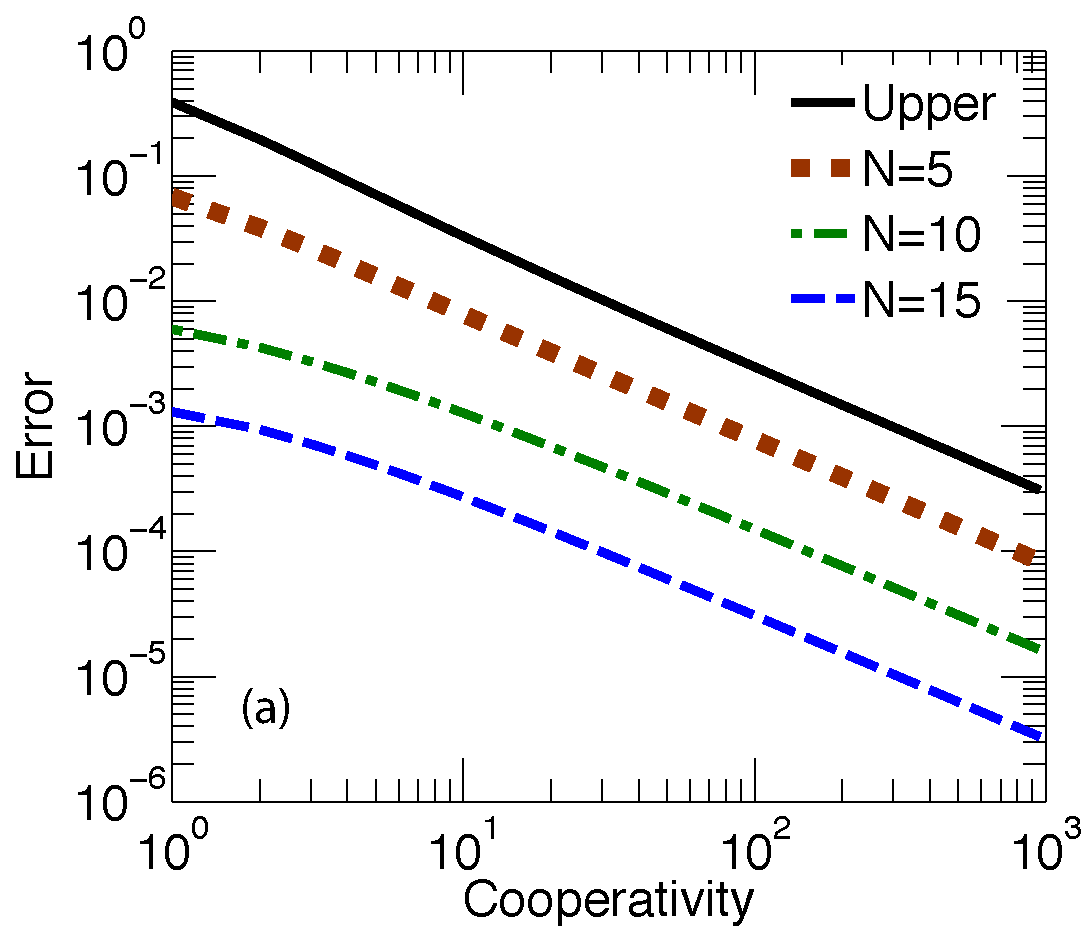
\includegraphics[width=0.46\textwidth]{./figs_Borregaard_PRL2015/figure2a}
\quad\quad
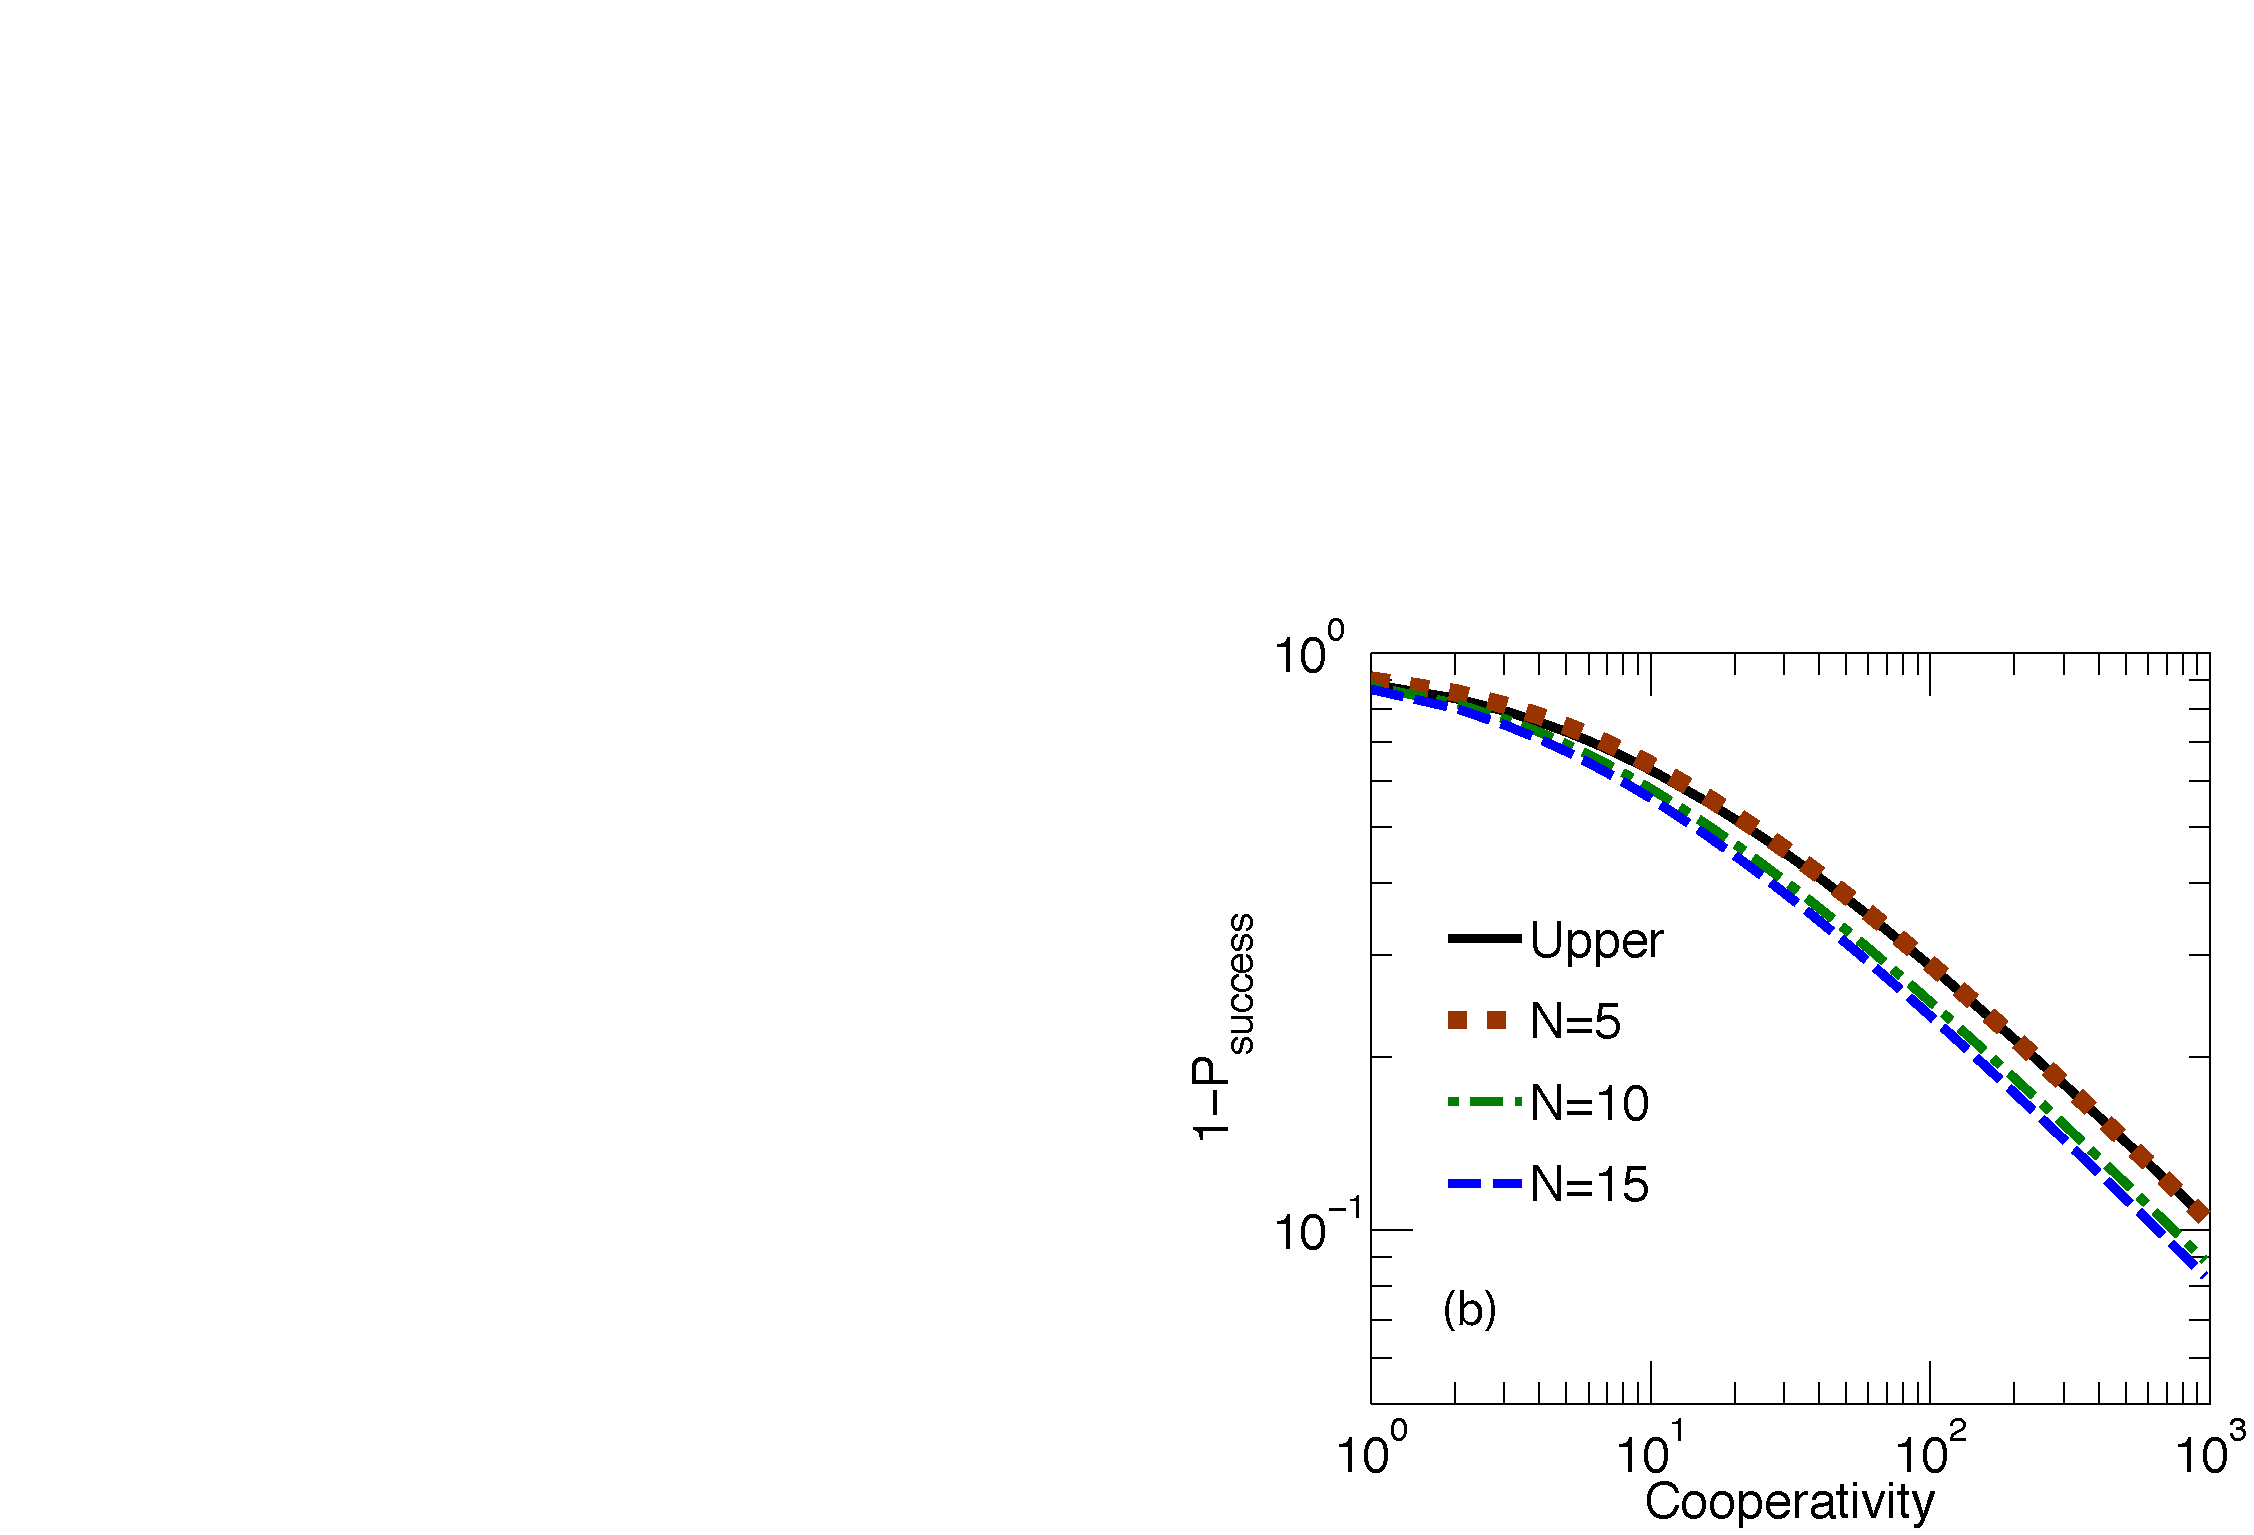
\includegraphics[width=0.46\textwidth]{./figs_Borregaard_PRL2015/figure2b}
\caption
[Error and success probability vs cooperativity]
{(a) Gate error of the Toffoli for different initial states as a
function of cooperativity. We have plotted the generic error for $N=5,10$, and 15 and the upper bound of the error. Note that the generic error decreases as $N$ increases. We have fixed $\Delta$ such that $\Gamma_{0}=\Gamma_{1}$ and have assumed that $\alpha=\beta=1$. (b) The failure probabilities $1-P_{\text{success,up}}$ and  $1-P_{\text{success,gen}}$ as a function of cooperativity. $1-P_{\text{success,gen}}$ is plotted for $N=5,10,15$. We have used the same assumptions as in (a). In general, the failure probability only have a weak dependence on $N$. Note that the line for $1-P_{\text{success, gen}},N=5$ coincides with  $1-P_{\text{success,up}}$.}
\label{fig:toffoli}
\end{figure}
As $N$ increases we obtain higher generic fidelity, whereas the success
probability is almost independent of $N$.

\subsection{CZ-gate}

In the special case of only two qubits the Toffoli gate is referred to as a
control-phase (CZ) gate. As shown in the article, we can, in this case,
completely remove the errors from the gate by choosing the detunings
$\Delta_{E}$ and $\Delta_{e}$ such that $\Gamma_{0}=\Gamma_{1}=\Gamma_{2}$ and
combining it with single qubit rotations we can ensure the right phase
evolution. In the general case where $\alpha,\beta\neq1$, the detunings
$\Delta_{e}$ and $\Delta_{E}$ are
\begin{eqnarray}
\Delta_{E}&=&\frac{\gamma}{2}\sqrt{\beta}\sqrt{4\alpha C+\beta} \\
\Delta_{e}&=&\frac{\alpha C\gamma^{2}}{2\Delta_{E}}. 
\end{eqnarray}
The success probability of the gate is then
\begin{equation}
P_{\text{success}}\simeq1-\pi\frac{8\beta^{2}+6\beta\alpha+\alpha^{2}}{8\beta^{3/2}\sqrt{\alpha}}\frac{1}{\sqrt{C}},
\end{equation} 
and we find that the gate time is
$t_{\text{CZ}}\simeq\frac{\gamma\pi\sqrt{\alpha}(\alpha+2\beta)(\alpha+4\beta)}{2\beta^{3/2}\Omega^{2}}\sqrt{C}$
in the limit $C\gg1$.
\subsection{Two-photon driving}

We now describe the details of the implementation where the auxiliary atoms is
driven by a two-photon process as shown in \reffig{fig:figureS2} (reproduced
from Fig. 4(a) in the article) in order to suppress the dominant undetectable
error caused by spontaneous decay of the auxilliary atom into the state
$\ket{g}$ ($\hat{L}_{g}$).

\begin{figure}
\centering
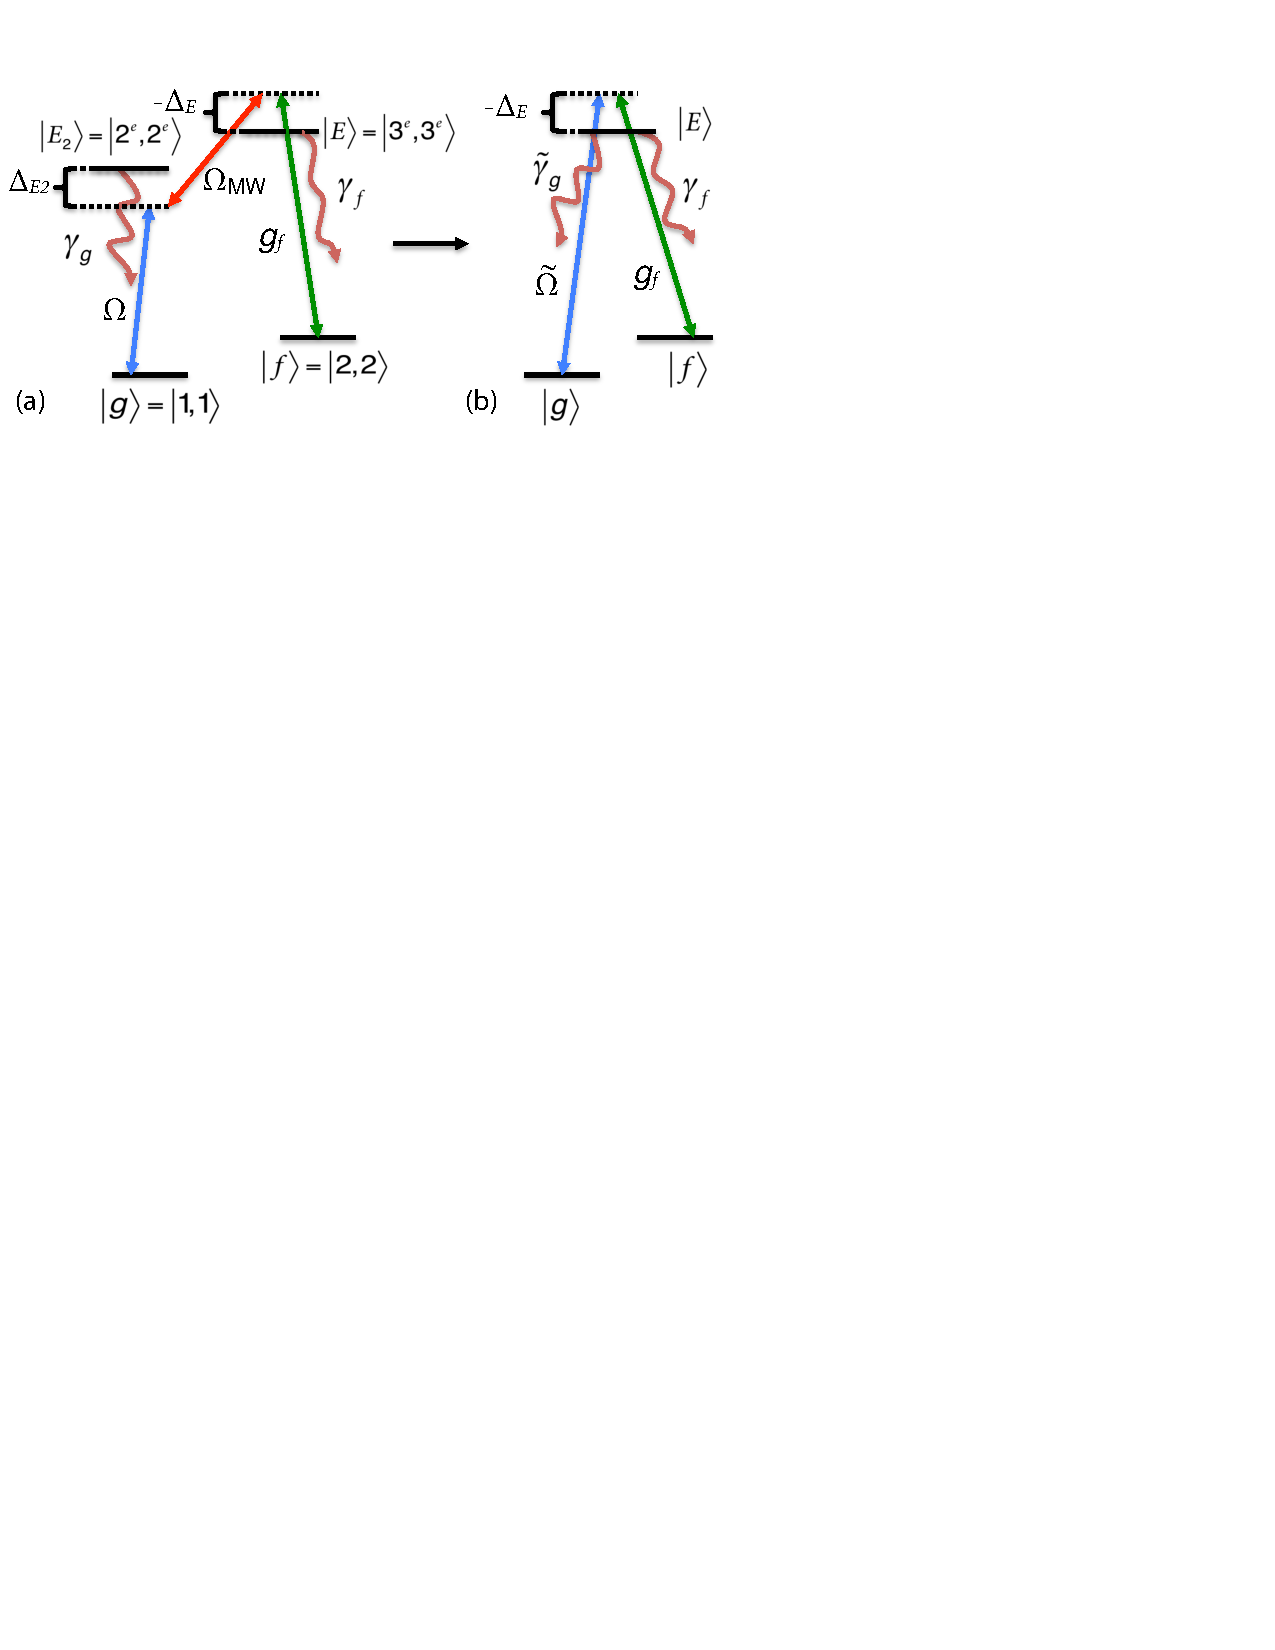
\includegraphics[width=0.7\textwidth]{./figs_Borregaard_PRL2015/figureS2} 
\caption 
[Level structure of auxiliary atom]
{(a) Level structure of the auxiliary atom and the transitions driven by
a weak laser ($\Omega$), a microwave field ($\Omega_{\text{MW}}$) and the cavity
($g_{f}$). We assume that $\ket{E}\leftrightarrow\ket{f}$ is a closed transition
and for simplicity we also assume that $\ket{E_{2}}\leftrightarrow\ket{g}$ is a
closed transition but this is not a necessity. The figure also indicates how the
levels could be realized in ${}^{87}$Rb. Here $\ket{r^{(e)},r^{(e)}}$ with
$r=1,2,3$ refers to state $\ket{\text{F}^{(e)}=r,\text{m}_{\text{F}}^{(e)}=r}$
in $5^{2}S_{1/2}$ $(5^{2}P_{3/2})$. (b) Effective three level atom realized by
mapping the two-photon drive to an effective decay rate $\tilde{\gamma}_{g}$ and
an effective drive $\tilde{\Omega}$}
\label{fig:figureS2}
\end{figure} 

The Hamiltonian in a proper rotating frame is
\begin{eqnarray} \label{eq:supphamil2}
\hat{H}&=&\hat{H}_{e}+\hat{V}+\hat{V}^{\dagger}, \\
\hat{H}_{e}&=&\Delta_{E}\ket{E}\bra{E}+\Delta_{E2}\ket{E_{2}}\bra{E_{2}}+g_{f}(\hat{a}\ket{E}\bra{f}+H.c)
\nonumber \\
&&+\frac{\Omega_{\text{MW}}}{2}(\ket{E}\bra{E_{2}}+H.c.) \nonumber \\
&&+\sum_{k}\Delta_{e}\ket{e}_{k}\bra{e}+g(\hat{a}\ket{e}_{k}\bra{1}+H.c.), \\
\hat{V}&=&\frac{\Omega}{2}\ket{E_{2}}\bra{g},
\end{eqnarray}  
where we have now defined
$\Delta_{E}=\omega_{E}-\omega_{g}-\omega_{laser}-\omega_{\text{MW}}$, 
$\Delta_{E2}=\omega_{E2}-\omega_{g}-\omega_{laser}$ and
$\Delta_{e}=\omega_{e}-\omega_{g}-\omega_{laser}-\omega_{\text{MW}}+\omega_{f}-\omega_{1}$.
Here $\omega_{laser}$ is the frequency of the laser drive ($\Omega$),
$\omega_{\text{MW}}$ is the frequency of the microwave field
($\Omega_{\text{MW}}$) and otherwise $\omega_{x}$ is the frequency associated
with level $x$. We assume that the frequency of the cavity is
$\omega_{c}=\omega_{laser}+\omega_{\text{MW}}+\omega_{g}-\omega_{f}$ such that
the three photon Raman transition from $\ket{g}\to\ket{f}$ is resonant. We have
assumed that $\Delta_{E2}$ is large and positive such that the rotating wave
approximation is valid for the microwave field.
The Lindblad operators describing the system are the same as described below
Eq.~\eqref{eq:hamil1} except that
$\hat{L}_{g}\to\sqrt{\gamma_{g}}\ket{g}\bra{E_{2}}$. Assuming a weak drive
$\Omega$, we can follow the same recipe as before to find the following
effective operators describing the dynamics of the system.
\bal
&&\hat{H}^{(2)}_{\text{eff}}
= \sum_{n=0}^{N}\Delta^{(2)}_{n}\ket{g}\bra{g} \otimes \hat{P}_{n}
\label{eq:supham3}\\
&&\qquad \Delta^{(2)}_{n} = \frac{-\Omega^{2}}{4\gamma}\mathrm{Re}
\left[\frac{\tilde{\Delta}_{e}(i\tilde{\Delta}_{E}/2+C_{f})+n
\tilde{\Delta}_{E}C}{\tilde{\Delta}_{E2}\tilde{\Delta}_{e}
(i\tilde{\Delta}_{E}/2+C_{f})+n\tilde{\Delta}_{E}\tilde{\Delta}_{E2}
C-i\tilde{\Delta}_{e}\tilde{\Omega}_{\text{MW}}^{2}/8-n
\tilde{\Omega}_{\text{MW}}^{2}C/4}\right]\nonumber
\\
&&\hat{L}_{0}^{\text{eff}(2)}=\sum_{n=0}^{N}r_{0,n}^{\text{eff}(2)}\ket{f}\bra{g}\otimes
\hat{P}_{n}
\label{eq:subleff3}\\
&&\qquad r_{0,n}^{\text{eff}(2)} =
\frac{-1}{4\sqrt{\gamma}}\frac{\sqrt{C_{f}}\tilde{\Delta}_{e}\Omega\tilde{\Omega}_{\text{MW}}}{\tilde{\Delta}_{E2}\tilde{\Delta}_{e}(i\tilde{\Delta}_{E}/2+C_{f})+n\tilde{\Delta}_{E2}\tilde{\Delta}_{E}C-i\tilde{\Delta}_{e}\tilde{\Omega}_{\text{MW}}^{2}/8-n\tilde{\Omega}_{\text{MW}}^{2}C/4}
\nonumber
\\
&&\hat{L}_{g}^{\text{eff}(2)}=\sum_{n=0}^{N}r_{g,n}^{\text{eff}(2)}\ket{g}\bra{g}\otimes
\hat{P}_{n}\\
&&\qquad r_{g,n}^{\text{eff}(2)} =
\frac{\Omega}{2}\frac{\tilde{\Delta}_{e}(i\tilde{\Delta}_{E}/2+C_{f})+n\tilde{\Delta}_{E}C}{\tilde{\Delta}_{E2}\tilde{\Delta}_{e}(i\tilde{\Delta}_{E}/2+C_{f})+n\tilde{\Delta}_{E2}\tilde{\Delta}_{E}C-i\tilde{\Delta}_{e}\tilde{\Omega}_{\text{MW}}^{2}/8-n\tilde{\Omega}_{\text{MW}}^{2}C/4}\frac{\sqrt{\gamma_{g}}}{\gamma}
\nonumber
\\
&&\hat{L}_{f}^{\text{eff}(2)} =
\sum_{n=0}^{N}r_{f,n}^{\text{eff}(2)}\ket{f}\bra{g} \otimes \hat{P}_{n}\\
&&\qquad r_{f,n}^{\text{eff}(2)} = 
-\frac{\Omega}{4}\frac{(i\tilde{\Delta}_{e}/2+nC)\tilde{\Omega}_{\text{MW}}}{\tilde{\Delta}_{E2}\tilde{\Delta}_{e}(i\tilde{\Delta}_{E}/2+C_{f})+n\tilde{\Delta}_{E2}\tilde{\Delta}_{E}C-i\tilde{\Delta}_{e}\tilde{\Omega}_{\text{MW}}^{2}/8-n\tilde{\Omega}_{\text{MW}}^{2}C/4}\frac{\sqrt{\gamma_{f}}}{\gamma}
\nonumber
\eal
\bal
&&\hat{L}_{k}^{\text{eff}(2)} =
\sum_{n=0}^{N-1}r_{n}^{\text{eff}(2)}\ket{f}\bra{g}\otimes\ket{\tilde{o}}_{k}\bra{1}\otimes
\hat{P}_{n}, \label{eq:subleff4} \\
&&\qquad r_{n}^{\text{eff}(2)} = 
\frac{1}{4\sqrt{\gamma}}\frac{\sqrt{C_{f}}\sqrt{C}\tilde{\Omega}_{\text{MW}}\Omega}{\tilde{\Delta}_{E2}\tilde{\Delta}_{e}(i\tilde{\Delta}_{E}/2+C_{f})+n\tilde{\Delta}_{E2}\tilde{\Delta}_{E}C-i\tilde{\Delta}_{e}\tilde{\Omega}_{\text{MW}}^{2}/8-n\tilde{\Omega}_{\text{MW}}^{2}C/4}
\nonumber
\eal
where we have defined the complex detuning
$\tilde{\Delta}_{E2}\gamma=\Delta_{E2}-i\gamma_{g}/2$ and the parameters
$r_{0,n}^{\text{eff}(2)},r_{g,n}^{\text{eff}(2)},r_{f,n}^{\text{eff}(2)}$ and
$r_{n}^{\text{eff}(2)}$ to characterize the decay described by the Lindblad
operators.

We are interested in the limit of large detuning $\Delta_{E2}$ and large
cooperativity $C$. In this limit, we find that the dynamics of the system can be
mapped to a simple three level atom with effective driving
$\tilde{\Omega}\sim\Omega\Omega_{\text{MW}}/(2\Delta_{E2})$ and an effective
decay $\tilde{\gamma}_{g}\sim\gamma_{g}\Omega_{\text{MW}}^{2}/\Delta_{E2}^{2}$
as shown in \reffig{fig:figureS2}. In principle, the effective operator
$\hat{L}_{0}^{\text{eff}(2)}$ leads to an effective decay rate of
$\tilde{\gamma}=\gamma_{g}\Omega^{2}/\Delta_{E2}^{2}$ to lowest order in $C$ 
but we find that this first order term do not destroy the coherence between the
qubit states since it is independent of $n$. There is, therefore, no effect of
these scattering events and the performance of the gate behaves as if there is
an effective decay rate of
$\tilde{\gamma}_{g}\sim\gamma_{g}\Omega_{\text{MW}}^{2}/\Delta_{E2}^{2}$. Note
that we also have an AC stark shift imposed on the level $\ket{g}$ by the laser
characterized by $\Omega$. This will give an overall phase to the system,
$\sim\Omega^{2}/(4\Delta_{E2})t$, which we can neglect since it does not
influence the gates.
Since we can do the mapping to the simple three level atom, we find similar
results for the performance of the gates for the two-photon scheme as for the
simple three level scheme only with effective decay $\tilde{\gamma}_{g}$ and
drive $\tilde{\Omega}$ given by the two-photon process. Note, however, that we
now assume $\gamma_{g}>0$, which introduces an undetectable error as previously
mentioned. We find that this introduces an error in the fidelity of both gates
of roughly
\begin{eqnarray}
&\sim&\frac{(\alpha^{2}-4\alpha\beta-6\beta^{2})\pi^{2}}{128\beta^{2}}\frac{\gamma_{g}^{4}}{\gamma^{4}\Delta_{E2}^{4}}+\frac{(\alpha^{2}+4\alpha\beta+6\beta^{2})\pi}{16\sqrt{\alpha\beta}(\alpha+2\beta)(\alpha+5\beta))}\frac{\gamma_{g}\Omega_{\text{MW}}^{2}}{\gamma\Delta_{E2}^{2}}\frac{1}{\sqrt{C}}\qquad.
\end{eqnarray}  
Nonetheless, this error can be suppressed arbitrarily much be increasing
$\Delta_{E2}$, which enable us to have a heralded CZ-gate with arbitrarily small
error in a realistic atomic setup using the two-photon drive.

\section{Gate time}
Here we address the question of how strongly we can drive the system and still
maintain the validity of perturbation theory. We need to adress this question
since the gate time depends inversely on the driving strength as shown in the
article and hence this limits the achievable gate time. A necessary criterion
for our pertubation theory to be valid is that the energy shifts $\Delta_{n}$
(see Eq.~\eqref{eq:supham2} and Eq.~\eqref{eq:supham3}) are small compared to
the driving, i.e. $\sim\Delta_{n}^{2}/\Omega^{2}\ll1$. From
Eq.~\eqref{eq:supham2} we find that
$\Delta_{n}^{2}/\Omega^{2}\sim\Omega^{2}/(16\Delta_{E}^{2})$ to leading order in
the cooperativity $C$ and this criterion is therefore met for
$\Omega\ll4\Delta_{E}$. Similarly, for the two-photon process, we find from
Eq.~\eqref{eq:supham3} that
$(\Delta_{n}^{(2)})^{2}/\Omega^{2}\sim\Omega^{2}/(16\Delta_{E2}^{2})$, to
leading order in $C$. Here we thus need $\Omega\ll4\Delta_{E2}$.

Another criterion need to be meet in order for our perturbative theory to be
valid. If none of the qubits couple, we are effectively driving the auxiliary
atom/cavity system into a dark state of the form
$\cos(\theta)\ket{0,g}-\sin(\theta)\ket{1,f}$, where the mixing angle is
$\theta\sim\Omega/g$. Here the number refers to the number of cavity photons. To
adiabatically eliminate the state $\ket{f,1}$ from the Hamiltonian as we have
done in the effective Hamiltonian requires that $\Omega/g\ll1$. Mapping this
criterion to the effective three level scheme realized in the two-photon scheme
gives $\Omega\Omega_{\text{MW}}/(2\Delta_{E2}g)\ll1$.

Finally, we need to consider the scattering of photons from the level $\ket{E2}$
in the two-photon scheme. If the number of scattering events, $n_{scat}$ is
large compared to $\Omega^{2}/(16\Delta_{E2}^{2})$, the perturbation theory is
not valid even though the other criterions are met. We find that
$n_{scat}\sim\frac{12\sqrt{C}\gamma^{2}}{\Omega_{\text{MW}}^{2}}$ for the
CZ-gate and we thus need to have 
$\frac{3\sqrt{C}\gamma^{2}\Omega^{2}}{\Delta_{E2}^{2}\Omega_{\text{MW}}^{2}}\ll1$

The different criterions for the validity of the perturbation theory are
summarized in \tabref{tab:tableS1}.
\begin{table} [H]
\centering
\begin{tabular}{|c|c|}
\hline
Simple scheme & Two-photon scheme  \\ \hline
$\Omega/(4\Delta_{E})\ll1$ & $\Omega/(4\Delta_{E2})\ll1$ \\ \hline
$\Omega/g\ll1$ & $\Omega\Omega_{\text{MW}}/(\Delta_{E2}g)\ll1$ \\ \hline
- & $3\sqrt{C}\gamma^{2}\Omega^{2}/(\Delta_{E2}^{2}\Omega_{\text{MW}}^{2})\ll1$  \\ \hline
\end{tabular}
\caption
[Perturbation validity criteria]
{The criterions for our perturbation theory to be valid. }
\label{tab:tableS1}
\end{table}
For all the gate schemes, we have assumed that
$\Delta_{E}\propto\sqrt{C}\gamma$. The first criterion for the simple scheme
(see \tabref{tab:tableS1}) can thus be met with a driving of
$\Omega=a\gamma\sqrt{C}$ where $a/4\ll1$. This driving results in a gate time
that decreases as $1/\sqrt{C}$. The value of $a$ will determine the size of the
non-adiabatic error. The second criterion is also fulfilled for this driving as
long as $\sqrt{\gamma/\kappa}\ll1$. In realistic systems such as the nanocavity
system described in Ref.~\cite{thompson, Tiecke}, the ratio $\kappa/\gamma$ can
be on the order of 100-1000.
For the two-photon scheme, we find from \tabref{tab:tableS1} that we can choose
$\Omega=a_{2}\Delta_{E2}, \Omega_{\text{MW}}=b\gamma C^{1/4}$ where the
constants $a_{2},b$ will determine the size of the non-adiabatic errors as
before. Similar to the situation in the simple scheme we assume that
$\sqrt{\gamma/\kappa}\ll1$.

\section{Numerical simulation}
In order to confirm our results, we numerically integrated the full Master
equation, defined by the Hamiltonian $\hat H$ and the Lindblad operators,
$\hat L_j \in \{\hat L_0, \hat L_g, \hat L_f, \hat L_1, \hat L_2\}$, 
\bel
\label{eq:full Master eq}
	\frac{d}{dt}\rho(t) = -\frac{i}{\hbar}[\hat H,\rho(t)]+\sum_j \frac{1}{2}
	\left[2 \hat L_j \rho(t) \hat L_j^{\dag} - \rho(t) \hat L_j^{\dag} \hat L_j -
	\hat L_j^{\dag} \hat L_j \rho(t)\right]
\eel
We used the QuTiP 2
package \cite{Johansson20131234}, for Python, to set up the problem and used its
12th-order numerical integration algorithm to find the solution $\rho(t)$ as a
time series.
Then, we used the routines of the same package to analyze the results. 

For each time series $\rho(t)$, we determined the gate time $t_{\text{gate}}$,
the success probability $P_{\text{success}}$, and the fidelity $F$.
We picked $\ket{\psi_0}_{12} =
\frac{1}{\sqrt{2}}\big(\ket{0} +
\ket{1}\big)_1\otimes\frac{1}{\sqrt{2}}\big(\ket{0}+ \ket{1}\big)_2$ as the
initial state of the two qubits, $\ket{g}$ for the control atom, and zero
photons in the cavity. Starting from here, we let the system evolve under the
Master equation Eq.~(\ref{eq:full Master eq}), and determined $P_g(t)$, the
conditional state $\rho_g(t)$ and $F(t)$ as a function of time:
\bal
	P_g(t) &=& \text{Tr}	\Big[\rho(t)\ket{g}\bra{g}\Big],
	\\
	\rho_g(t) &=& \frac{\ket{g}\bra{g}\rho(t)
	\ket{g}\bra{g}}{P_g(t)},
	\\
	F(t) &=& \max_{\phi_1, \phi_2}\Ev{\left.\psi_t^{\phi_1, \phi_2}\right|
	\text{Tr}_{\text{c, c}}\big(\rho_g(t)\big) \left| \psi_t^{\phi_1,
	\phi_2}\right.}
% 	E(t) &=& \text{Ent}\big(\;P_{\text{logical}}\;
% 	\text{Tr}_\text{control, cav}\big(\rho_g(t)\big)\;P_{\text{logical}}
% 	/\mathcal{N}\;\big),
\eal
where $\text{Tr}_{\text{c, c}}$ is the partial trace operation over
the control atom and the cavity, and $\ket{\psi_t^{\phi_1, \phi2}}$ is the
target state transformed with two single qubit $z$-rotations:
\bel
	\Ket{\psi_t^{\phi_1, \phi_2}} = \hat U_1(\phi_1) \hat U_2(\phi_2)
	\frac{1}{2}\Big(\ket{00} + \ket{01} + \ket{10} - \ket{11}\Big),
\eel
where $\hat U_{k}(\phi_k) = \exp\left[i \ket{1}_k\bra{1}_k \phi_k\right]$ is the
$z$-rotation of qubit $k$ ($= 1,2$) by the angle $\phi_k$.
% $P_\text{logical} =
% \ket{00}\bra{00} + \ket{01}\bra{01} + \ket{10}\bra{10} + \ket{11}\bra{11}$
% is the projector onto the logical subspace of the qubits, and $\mathcal{N}$ is a
% normalization constant.
% $\text{Ent}(\rho)$ of a two-qubit density matrix $\rho$
% is defined, according to \cite{Wootters1998}, as
% $
% 	\text{Ent}(\rho) = h\Big[\Big(1 + \sqrt{1-c^2(\rho)}\Big) /2\Big],
% $
% where $h(x) = -x\log_2 (x) - (1-x)\log_2(1-x)$, and $c(\rho)$ is the
% concurrence of $\rho$. We then determined the gate time $t_\text{gate}$ by
% finding the timepoint where $E(t)$ is maximal. 
From these time series, we determined the gate time $t_{\text{gate}}$ by
finding the timepoint where $F(t)$ is maximal,
\bel
	t_{\text{gate}} = \underset{t}{\text{argmax}}\;F(t)
\eel
 The fidelity and the success
probability of the gate is then defined as $F = F(t_{\text{gate}})$,
$P_{\text{success}} = P_g(t_{\text{gate}})$. 
% We chose to evaluate the fidelity
% through entanglement $E$, since it can be determined without the knowledge of
% the exact single-qubit rotations required to complete the gate, which are
% always easier to perform than two-qubit operations.

Plots of Fig.~\ref{fig:t_gate,P_success} show the gate time ($t_{\text{gate}}$)
and the success probability ($P_{\text{success}}$) as a function of $a$, for
$\gamma_g = 0$, $\gamma = 0.01\kappa$, $\Omega=a\gamma\sqrt{C}$ with
$C\in\{10,30,100,300,1000\}$. The detunings, $\Delta_E$ and $\Delta_e$ were
chosen to be close to their optimal value, determined from the adiabatic theory,
and numerically optimized to result in identical effective $\ket{g}\rightarrow
\ket{f}$ transition rates  $\Gamma_0 = \Gamma_1 = \Gamma_2$ for the qubit
sectors $\ket{00}, \ket{01}, \ket{11}$. The rates $\Gamma_j$ were found by
numerically diagonalizing the master equation for the qubit sectors separately,
and finding the eigenvalue with the smallest (but non-zero) absolute real part.
This numerical optimization yielded the maximal fidelity. The symbols correspond
to the numerical result, whereas the solid lines show the theoretical values.
The agreement of the results confirms the validity of the adiabatic theory for a
driving $\Omega=a\gamma\sqrt{C}$ for $C\lesssim 1000$ and $a\lesssim0.25$. Note,
however, that Fig.~\ref{fig:t_gate,P_success} shows how the success probability
deviates from the adiabatic result for $a\gtrsim0.25$. A weak increase of this
deviation with the cooperativity is seen but from simulations at high C, we
believe that this can be removed by gradually ramping $\Omega$ up and down to
maintain adiabaticity at the beginning and end of the driving pulse. This was
not included in the simulations behind Fig.~\ref{fig:t_gate,P_success} for
simplicity.
 \begin{figure}[h]
\centering
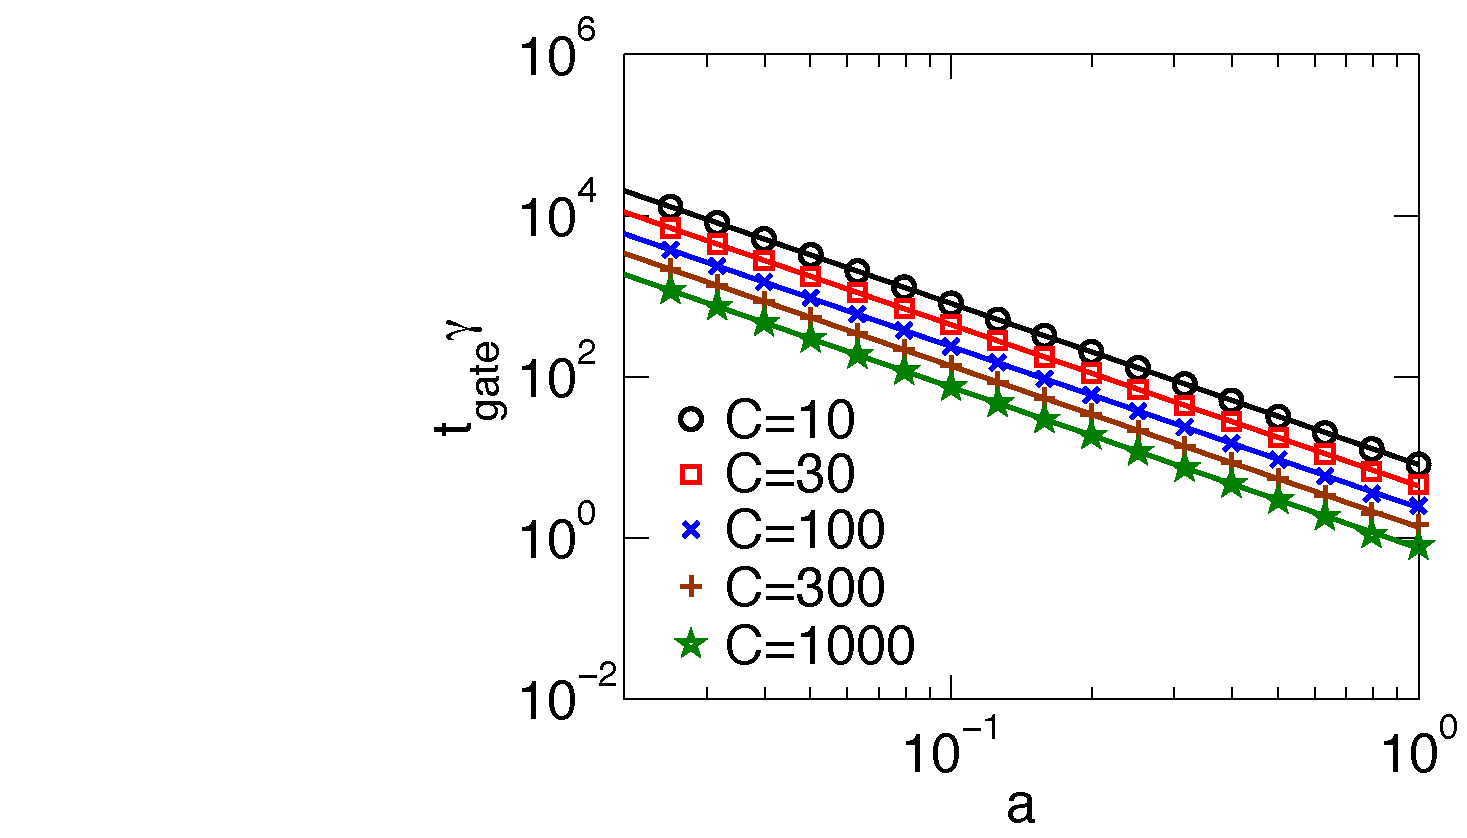
\includegraphics[width=0.48\textwidth]{./figs_Borregaard_PRL2015/figureSN1}\quad 
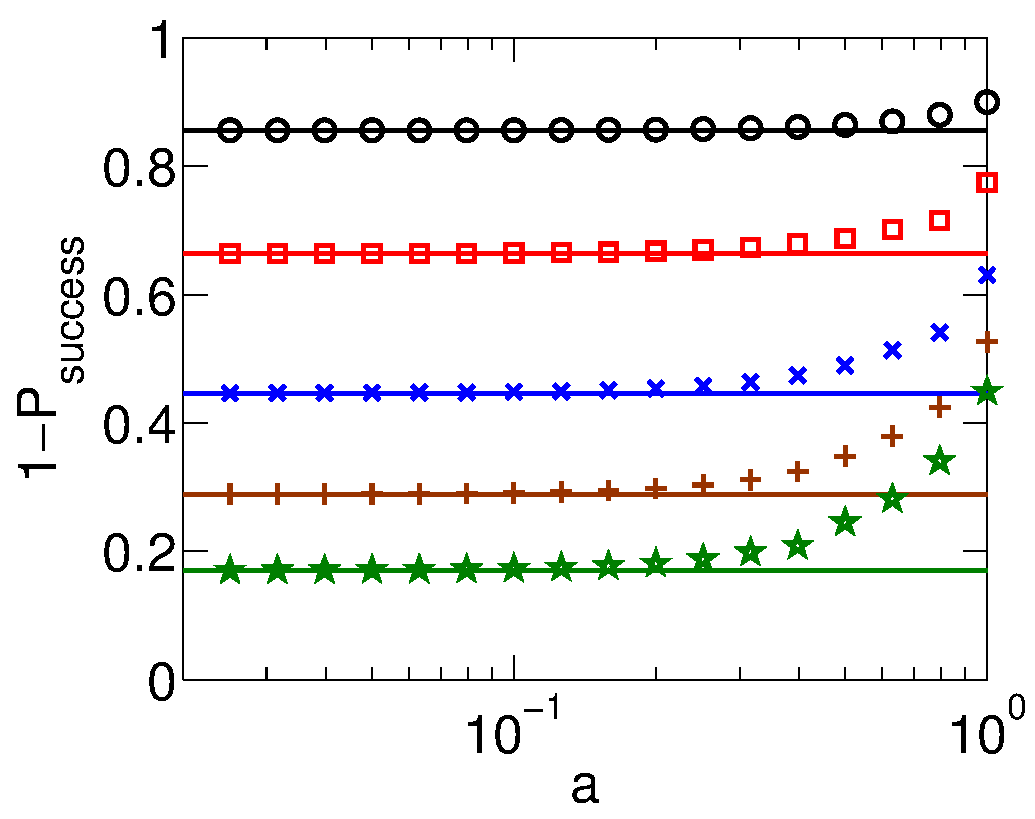
\includegraphics[width=0.48\textwidth]{./figs_Borregaard_PRL2015/figureSN2}
\caption
[Gate time and success probability vs driving strength]
{
\label{fig:t_gate,P_success}
Gate time (left) and failure probability (right) as a function of driving
strength ($a$) for $\gamma/\kappa = 0.01$, $\gamma_g = 0$, and
$C\in\{10,30,100,300,1000\}$. The driving strength was assumed to be
$\Omega=a\gamma\sqrt{C}$.}
\end{figure} 
 
Fig.~\ref{fig:F} shows the conditional \emph{in}fidelity of the gate as a
function of $a$ for the same parameters. The simulation confirms that using $a =
0.25$ is enough to push the (conditional) infidelity of the gate below
$4\cdot10^{-5}$. The fidelity is limited by non-adiabatic effects, which can be
suppressed by decreasing $\Omega$ as shown in the figure. Adiabatically ramping
Ω up and down at the beginning and end of the gate will also improve the
adiabaticity but, for simplicity, we have not included this in the simulations
described here. Note, however that for high $C$ ($C>1000$), we find that this
gradual ramping of $\Omega$ significantly decreases the non-adiabatic error.
\begin{figure}[h] 
\centering
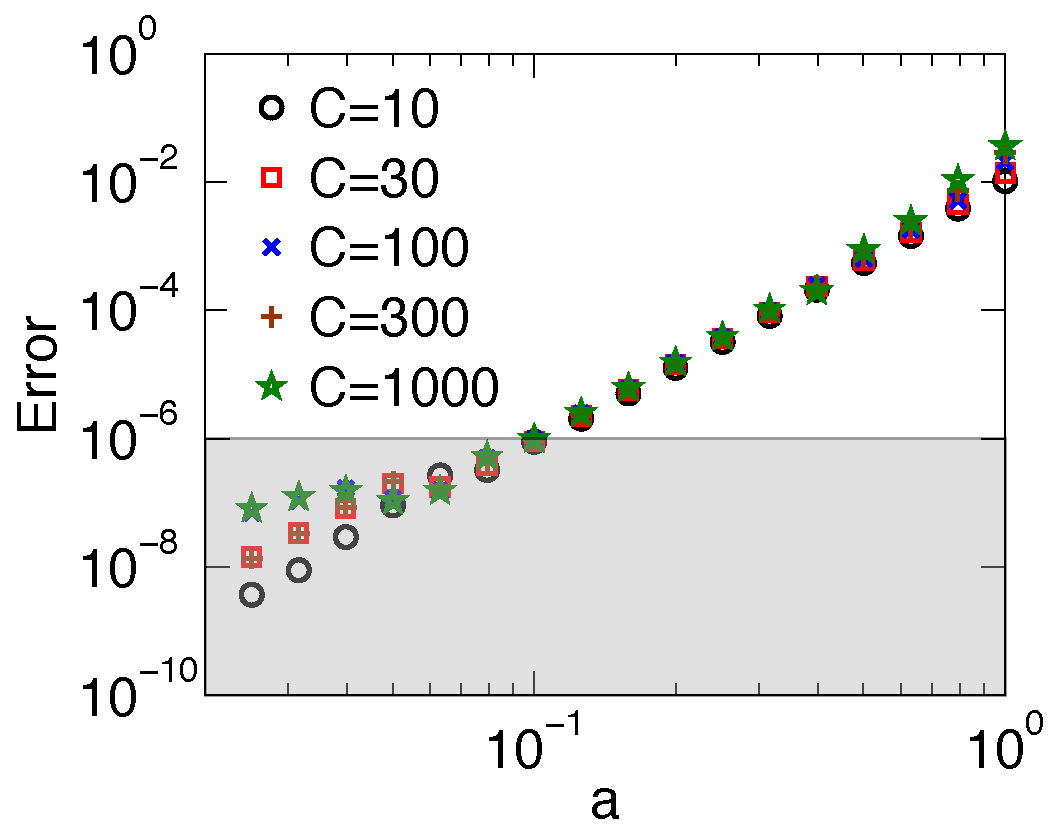
\includegraphics[width=0.5\textwidth]{./figs_Borregaard_PRL2015/figureSN3} 
\caption
[Conditional fidelity]
{ 
\label{fig:F}
Conditional infidelity of the gate as a function of the driving strength $(a)$
for $\gamma/\kappa = 0.01$, $\gamma_g = 0$, and $C\in\{10,30,100,300,1000\}$.
The shaded region (at $\sim 10^{-6}$) shows the limit of numerical accuracy. The
driving strength was assumed to be $\Omega=a\gamma\sqrt{C}$.}
\end{figure} 

We repeated the above analysis for the two-photon-driving Hamiltonian in
Eq.~\eqref{eq:supphamil2}. We chose $ \gamma = \gamma_g = \gamma_f =
0.01\,\kappa$,  $\Omega = \frac{\Delta_{E2}}{8 C^{1/4}}$, and
$\Omega_{\text{MW}} = 4\gamma C^{1/4}$, and chose $\Delta_E$ and $\Delta_e$
detunings again close to their adiabatic optimum, but numerically optimized them
with the same procedure as previously.
Plots of Fig.\ref{fig:t,P 2} show the gate time and the success probability as a
function of $\Delta_{E2}$ for $C\in\{10, 20, 50,100\}$. Symbols indicate the
numerical results while solid lines show the theoretical values.
 \begin{figure}[h]
\centering
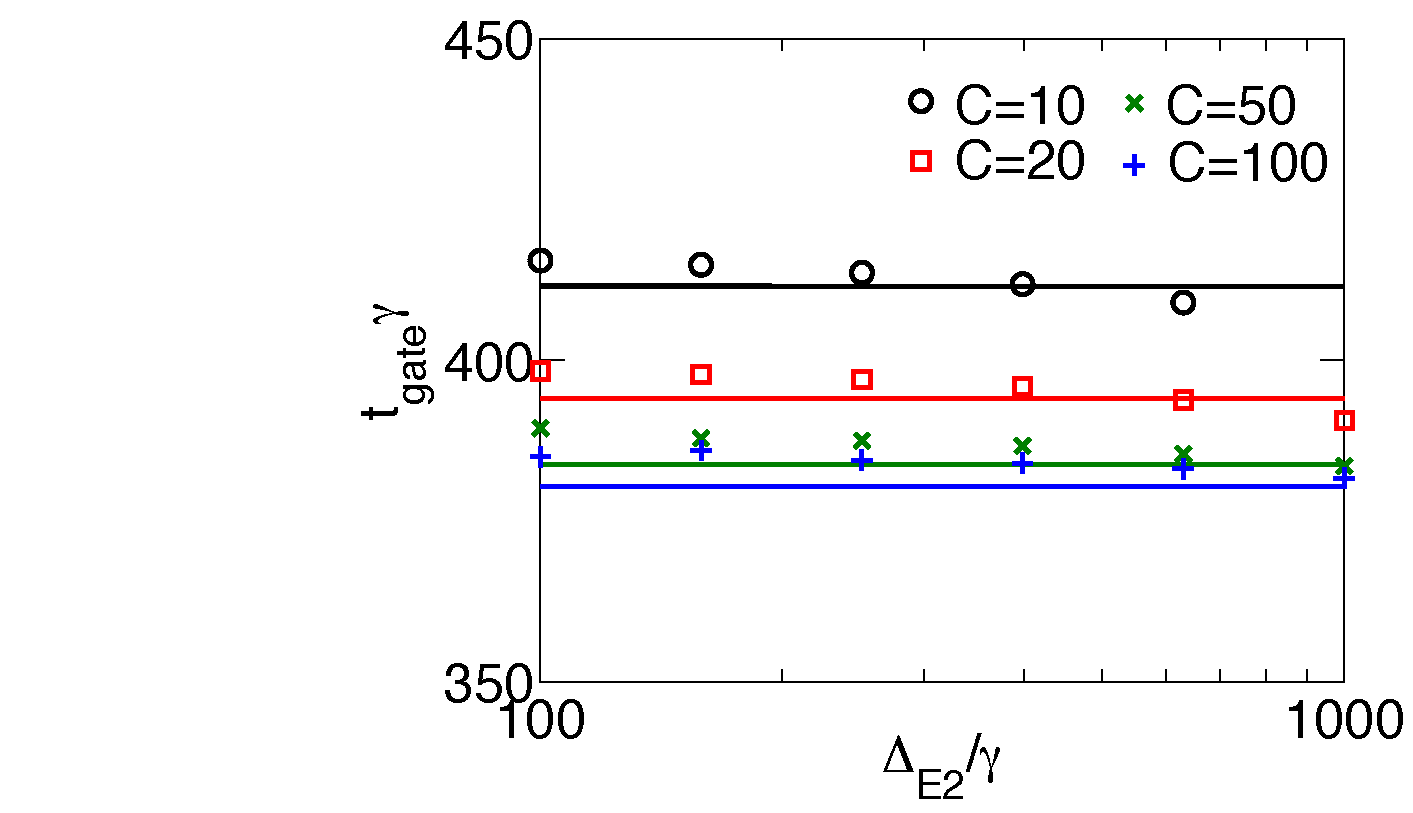
\includegraphics[width=0.48\textwidth]{./figs_Borregaard_PRL2015/figureSN4}\quad 
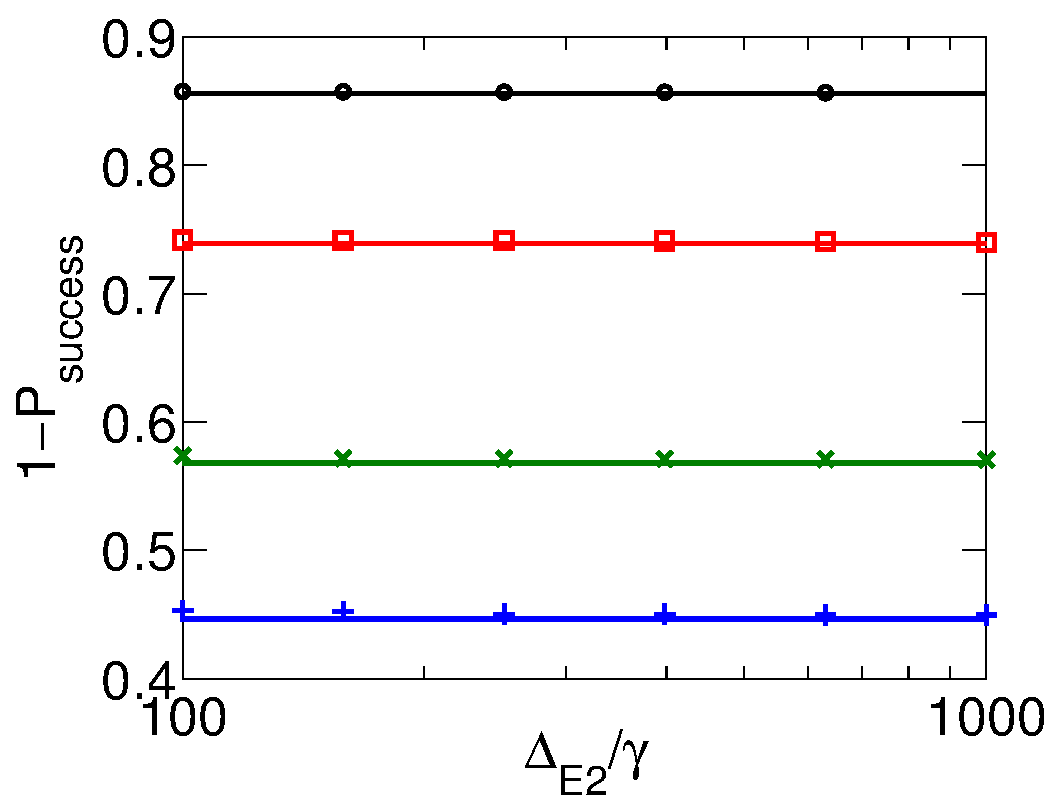
\includegraphics[width=0.48\textwidth]{./figs_Borregaard_PRL2015/figureSN5}
\caption
[Gate time and success probability vs detuning]
{
\label{fig:t,P 2} 
Gate time (left) and failure probability (right) as a function of $\Delta_{E2}$
for $\gamma = \gamma_g = \gamma_f = 0.01\kappa$, $\Omega = \frac{\Delta_{E2}}{8
C^{1/4}}$, $\Omega_{\text{MW}} = 4\gamma C^{1/4}$, $C = \{10,20,50,100\}$.
	}
\end{figure} 
Fig.~2b in the article shows the conditional \emph{in}fidelity of the
two-photon-driven gate as a function of $C$ for the same choice of parameters.
With these results, we confirm that by increasing $\Delta_{E2}$ we can lower the
infidelity error to an arbitrary small level. The gate time is a constant of the
cooperativity since we have increased $\Omega_{MW}$ as $C^{1/4}$ in the
simulations. We do see some deviation from the analytical results due to
non-adiabatic effects, which could be suppressed by decreasing $\Omega$ at the
expense of an increase in the gate time. Finally a gradual ramping of $\Omega$
could also decrease the non-adiabatic errors but for simplicity, we have not
included this in the simulations.

\section{Additional errors} 

There are some additional errors in a realistic atomic setup that we have not
treated in detail so far. Here we estimate the dominant errors and determine
under which conditions, they can be sufficiently suppressed such that they do
not limit the performance of the gates. We assume a realistic atomic setup where
${}^{87}$Rb atoms are used both for the auxiliary atom and the qubit atoms. In
the ${}^{87}$Rb atoms, we assume that $\ket{g}=\ket{1,1}, \ket{f}=\ket{2,2}$ and
$\ket{E_{2}}=\ket{2^{e},2^{e}}, \ket{E}=\ket{3^{e},3^{e}}$ where
$\ket{r^{(e)},r^{(e)}}$ with $r=1,2,3$ refers to state
$\ket{\text{F}^{(e)}=r,\text{m}_{\text{F}}^{(e)}=r}$ in $5^{2}S_{1/2}$
$(5^{2}P_{3/2})$. In this case, we estimate that the dominant errors are:
\begin{itemize}
\item In our perturbative theory, we have assumed that the laser field ($\Omega$) only couple $\ket{g}\to\ket{E2}$ in the auxiliary atom. However, for a large detuning $\Delta_{E2}$ it may also couple $\ket{f}\to\ket{E}$, which could lead to an undetectable error where the auxiliary atom is pumped back to $\ket{E2}$ from, which it decays to $\ket{g}$. This error is, however, suppressed by the large frequency separation, $\Delta_{g}$ of $\ket{g}$ and $\ket{f}$, which is $\Delta_{g}\sim1000\gamma$ for ${}^{87}$ Rb. We estimate the error using effective operators to find the decay rate back to $\ket{g}$, assuming that the auxiliary atom starts in $\ket{E2}$ and treating the drive $\Omega$ as a perturbation while neglecting the cavity coupling. This is valid as long as $\Delta_{g}\gg\Delta_{E}$, which is fulfilled for $C\lesssim10000$ since $\Delta_{E}\sim\sqrt{C}$. The error increases with $\Delta_{E2}$ but even for $\Delta_{E2}\approx400\gamma$ we find that for $\Omega_{\text{MW}}=4\gamma C^{1/4}$, $\Omega=\Delta_{E2}/8$ the error is $\lesssim10^{-4}$.     

\item The microwave might also couple the ground states $\ket{0}-\ket{1}$ of the
qubit atoms and the ground states $\ket{g}-\ket{f}$ of the auxiliary atom. The
coupling of $\ket{0}-\ket{1}$ means that the qubit atoms also couple to the
cavity even though they are in state $\ket{0}$. We estimate the error from this
to be on the order of
$\Omega_{\text{MW}}^{2}/(\Delta_{g}-(\Delta_{E2}-\Delta_{E}+\Delta_{2\to3}))^2$
where $\Delta_{2\to3}$ is the splitting between $\ket{E_{2}}$ and $\ket{E}$. For
${}^{87}$Rb, $\Delta_{2\to3}\approx44\gamma$. Below we argue that we need
$\Delta_{E}<0$. Since $\Delta_{E}\approx-\sqrt{C}\gamma$ this error will
increase slowly with cooperativity but it is suppressed by $\Delta_{g}$. For
$\Omega_{\text{MW}}=4\gamma C^{1/4}$, we find that the error is
$\lesssim10^{-4}$ for $C\lesssim1000$ even for $\Delta_{E2}\approx400\gamma$.
The errors from the coupling of the states $\ket{g}-\ket{f}$ in the auxiliary
atom will likewise be suppressed by the large energy splitting $\Delta_{g}$.
These errors can also be further suppressed by decreasing $\Omega_{\text{MW}}$
at the cost of a larger gate time.
\end{itemize}

The above errors can be highly suppressed using e.g.${}^{88}$Sr,
${}^{138}$Ba${}^{+}$ or ${}^{40}$Ca${}^{+}$ instead of ${}^{87}$Rb. For these
atoms, the ground states can be encoded in the $S_{0}$ and $P_{0}$ manifoldes
for ${}^{88}$Sr and the $S_{1/2}$ and $D_{3/5}$ manifolds for
${}^{138}$Ba${}^{+}$ and ${}^{40}$Ca${}^{+}$, which have separations at optical
frequencies between the stable states.

A final error that we will consider is that the transition
$\ket{E}\leftrightarrow\ket{f}$ will not be completely closed if the cavity is
linearly polarized. This will, e.g. be the case for the system in Ref.
\cite{thompson}. Such a cavity also couples $\ket{f}$ to the states
$\ket{1^{e},1^{e}},\ket{2^{e},1^{e}}$ and $\ket{3^{e},1^{e}}$. From
$\ket{1^{e},1^{e}}$ and $\ket{2^{e},1^{e}}$ there might be an undetectable decay
back to $\ket{g}$, which will introduce an error $\propto1/\sqrt{C}$ in the
gates. The probability of an undetectable decay from these states should be
compared to the probability of the detectable decays where the cavity photon is
scattered of the qubit atoms instead. For ${}^{87}$Rb, we estimate this error by
compairing the strengths of the effective couplings from $\ket{f}$ to
$\ket{1^{e},1^{e}}$ and $\ket{2^{e},1^{e}}$ with a subsequent decay to $\ket{g}$
with the strength of the effective coupling from $\ket{1}$ to $\ket{e}$ in the
qubit atoms with a subsequent decay back to $\ket{1}$. The latter process has a
detuning of $\Delta_{E}$ while the first two are additional detuned by the
energy gaps between $\ket{3^{e},3^{e}}$ and $\ket{1^{e},1^{e}}$ and
$\ket{3^{e},3^{e}}$ and $\ket{2^{e},1^{e}}$ respectively, assuming that
$\Delta_{E}<0$. We find that since $\abs{\Delta_{E}}$ grows as $\sqrt{C}$ the
error increases from $\sim5\cdot10^{-5}$ at $C=1$  to a maximum value of
$\sim2\cdot10^{-3}$ for $C\sim3000$ for which $\Delta_{E}$ is comparable to the
extra detunings of the $\ket{1^{e},1^{e}}$ and $\ket{2^{e},1^{e}}$ transitions
compared to the $\ket{e}$ transition. For $C>3000$ the error decreases as
$1/\sqrt{C}$.
Note that this error could be removed  by making a 4 photon drive from $\ket{g}$
to $\ket{E}$ by letting $\ket{g}=\ket{1,-1}$. Another approach is to consider
other atoms such as ${}^{40}$Ca${}^{+}$, with more favorable levelstructures.
The state $\ket{g}$ could be encoded in the $3^{2}D_{5/2}$ subspace while the
state $\ket{f}$ could be encoded in the $4^{2}S_{1/2}$ subspace and similarly
for the qubit states $\ket{0}$ and $\ket{1}$. In such a setup, we will have
separations of optical frequencies between the qubit states and we can remove
the decay from the excited state back to $\ket{g}$ by, e.g. driving from
$3^{2}D_{5/2}$ to $4^{2}P_{1/2}$ through $3^{2}D_{3/2}$.

\chapter{Appendices for Chapter \ref{ch:Borregaard_PRA2015}}
\label{app:Borregaard_PRA2015}

\section{Error analysis of the single-photon scheme} \label{single}

The setup of the single-photon scheme is described in Sec. \ref{sec:1phot}. The
single photon detectors are assumed to have a dark count probability of
$P_{\text{dark}}$ and an efficiency of $\eta_{\text{d}}$ while the transmission
efficiency of the fibers is denoted $\eta_{\text{f}}$.  As described in Sec.
\ref{sec:generation}, the probability of an emitter to go from the excited
state, $\ket{e}$ to the ground state $\ket{1}$ is $P_{\text{phot}}$ while the
excitation probability is $\epsilon^{2}$. The scheme is conditioned on a single
click at the central station. Depending on which detector gave the click, a
single qubit rotation can be employed such that ideally the state
$\ket{\Psi^{+}}$ is created. Going through all the possibilities of obtaining a
single click at the central station, we find that the density matrix following a
single click, and possible subsequent single qubit rotations, is
\begin{eqnarray}
\rho_{1click}&=&F_{1}\ket{\Psi^{+}}\bra{\Psi^{+}}+
\alpha_{1}\ket{\Phi^{+}}\bra{\Phi^{+}}+\alpha_{1}
\ket{\Phi^{-}}\bra{\Phi^{-}}\qquad\nonumber
\\
&&+\beta_{1}\ket{\Psi^{-}}\bra{\Psi^{-}}+
\tilde{\alpha}_{1}\ket{00}\bra{00}+ \tilde{\beta}_{1}\ket{11}\bra{11},
\end{eqnarray}
with coefficients
\begin{eqnarray}
&&F_{1}=\frac{1}{P_{\text{1click}}}
\Big[2\eta_{\text{d}}\eta_{\text{f}}P_p
\epsilon^{2}(1-\epsilon^{2})(1-P_d)
+2\eta_{\text{f}}(1-\eta_{\text{d}})P_p
\epsilon^{2}(1-\epsilon^{2})P_d(1-P_d)\nonumber
\\
&&\qquad+\frac{1}{2}\eta_{\text{d}}\eta_{\text{f}}P_p
\epsilon^{4}(1-P_p(1-P_d)+2(1-\eta_{\text{f}})P_p\epsilon^{2}(1-
\epsilon^{2})P_d(1-P_d) \nonumber \\
&&\qquad+(1-\eta_{\text{d}}\eta_{\text{f}})P_p
\epsilon^{4}(1-P_p)P_d(1-P_d)+(1-\epsilon^{2})\epsilon^{2}(1-P_p)
P_d(1-P_d)\nonumber
\\
&&\qquad+\frac{1}{2}\epsilon^{2}(1-P_p)^{2}
P_d(1-P_d)\Big] 
\\
&&\alpha_{1}=\frac{1}{P_{\text{1click}}}\Big[\frac{1}{2}
\epsilon^{2}(1-P_p)^{2}P_d (1-P_d)\Big]
\\
&&\beta_{1}=\frac{1}{P_{\text{1click}}}\Big[\frac{1}{2}\eta_{\text{d}}
\eta_{\text{f}}P_p\epsilon^{4}(1-P_p)
(1-P_d) +2(1-\eta_{\text{f}})P_p\epsilon^{2}
(1-\epsilon^{2})P_d(1-P_d) \nonumber \\
&&\qquad+(1-\eta_{\text{d}}\eta_{\text{f}})P_p
\epsilon^{4}(1-P_p)P_d(1-P_d)
+(1-\epsilon^{2})\epsilon^{2}(1-P_p)
P_d(1-P_d) \nonumber \\
&&\qquad+\frac{1}{2}\epsilon^{2}(1-P_p)^{2}
P_d(1-P_d) 
+2\eta_{\text{f}}(1-\eta_{\text{d}})P_p
\epsilon^{2}(1-\epsilon^{2})P_d(1-P_d)\Big] 
\\
&&\tilde{\alpha}_{1}=\frac{1}{P_{\text{1click}}}
\Big[2(1-\epsilon^{2})^{2}P_d(1-P_d)
+2(1-\epsilon^{2})\epsilon^{2}(1-P_p)
P_d(1-P_d)\Big] 
\\
&&\tilde{\beta}_{1}=\frac{1}{P_{\text{1click}}}
\Big[\eta_{\text{d}}\eta_{\text{f}}P_p
\epsilon^{4}(1-P_p)(1-P_d)
+2(1-\eta_{\text{d}}\eta_{\text{f}})P_p
\epsilon^{4}(1-P_p)P_d(1-P_d) \nonumber \\
&&\qquad +2(1-\eta_{\text{d}}\eta_{\text{f}})^{2}
P_p^{2}\epsilon^{4}P_d(1-P_d)
+2(1-\eta_{\text{d}}\eta_{\text{f}})
\eta_{\text{d}}\eta_{\text{f}}P_p^{2}
\epsilon^{4}(1-P_d)^{2}\Big],
\end{eqnarray}
where $P_d = P_{\text{dark}}$ and $P_p = P_{\text{phot}}$.
Here we have assumed that with probability $\epsilon^{2}(1-P_{\text{phot}})$, an
emitter is excited but spontaneously decay to the ground states instead of
emitting a cavity photon. Furthermore, we have assumed that the decay rates to
the two ground states are equal such that the emitter ends up in
$\frac{1}{2}(\ket{0}\bra{0}+\ket{1}\bra{1})$. Note that the detectors are not
assumed to be number resolving.  $P_{\text{1click}}$ is the total success
probability given by
\begin{eqnarray}
P_{\text{1click}}&=&2\eta_{\text{d}}
\eta_{\text{f}}P_{\text{phot}}\epsilon^{2}
(1-P_{\text{phot}}\epsilon^{2})(1-P_{\text{dark}})
+(2\eta_{\text{f}}\eta_{\text{d}}-
\eta_{\text{f}}^{2}\eta_{\text{d}}^{2}) P_{\text{phot}}^{2}\epsilon^{4}
\nonumber \\
&&+2(1-\epsilon^{2}P_{\text{phot}})^{2}
P_{\text{dark}}(1-P_{\text{dark}}) +2(1-\eta_{\text{d}}\eta_{\text{f}})^{2}
P_{\text{phot}}^{2}\epsilon^{4}P_{\text{dark}}(1-P_{\text{dark}})\nonumber \\
&&+4(1\!-\!\eta_{\text{d}}\eta_{\text{f}}) P_{\text{phot}}\epsilon^{2}
(1\!-\!\epsilon^{2}P_{\text{phot}}) P_{\text{dark}}(1\!-\!P_{\text{dark}}).
\end{eqnarray}
Assuming $P_{\text{dark}}\ll1$, the dominant error is where both qubits are
excited but only a single click is detected at the central station. This leaves
the qubits in the state $\ket{11}\bra{11}$ and this error is efficiently
detected by the purification scheme described in Ref. \cite{bennett}.

\section{Error analysis of the two-photon scheme} \label{two}

For the two photon scheme described in Sec. \ref{sec:generation}, we condition
on a click in two detectors. Once again we assume that appropriate single qubit
rotations are employed depending on which detector combination clicked such that
ideally the state $\ket{\Phi^{+}}$ is created. We find that the density matrix
describing the qubit state after a successful event is
\begin{eqnarray}
\rho_{2click}&=&F_{2}\ket{\Phi^{+}}\bra{\Phi^{+}}+\alpha_{2}\ket{\Psi^{+}}
\bra{\Psi^{+}}+\alpha_{2}\ket{\Psi^{-}}\bra{\Psi^{-}}+\beta_{2}\ket{\Phi^{-}}\bra{\Phi^{-}},
\end{eqnarray} 
where we have defined
\begin{eqnarray}
F_{2}&=&\frac{(1-P_{\text{dark}})^{2}}{P_{\text{2click}}}
\Big[\frac{1}{2}\eta_{d}^{2}\eta_{\text{f}}^{2}P_{\text{phot}}^{2} 
+\eta_{\text{d}}(1-\eta_{\text{d}})\eta_{\text{f}}^{2}
P_{\text{dark}}P_{\text{phot}}^{2}
+\eta_{\text{f}}^{2}(1-\eta_{\text{d}})^{2}P_{\text{phot}}^{2}
P_{\text{dark}}^{2}\nonumber \\
&&+P_{\text{dark}}^{2}(1-P_{\text{phot}})^{2}+\eta_{\text{d}}
(1-\eta_{\text{f}})\eta_{\text{f}}P_{\text{dark}}P_{\text{phot}}^{2}
+\eta_{\text{d}}\eta_{\text{f}}P_{\text{dark}}P_{\text{phot}}
(1-P_{\text{phot}})\nonumber \\
&&+(1-\eta_{\text{f}})^{2}P_{\text{phot}}^{2}P_{\text{dark}}^{2}
 +2\eta_{\text{f}}(1-\eta_{\text{d}})(1-\eta_{\text{f}})
P_{\text{phot}}^{2}P_{\text{dark}}^{2}\nonumber \\
&&+2(1-\eta_{\text{d}}\eta_{\text{f}})P_{\text{phot}}
(1-P_{\text{phot}})P_{\text{dark}}^{2}\Big]  
\\
\alpha_{2}&=&\frac{(1-P_{\text{dark}})^{2}}{P_{\text{2click}}}
\Big[\eta_{d}(1-\eta_{\text{f}})\eta_{\text{f}}P_{\text{dark}}
P_{\text{phot}}^{2} +P_{\text{dark}}^{2}(1-P_{\text{phot}})^{2}+\nonumber \\
&&\eta_{\text{d}}
\eta_{\text{f}}P_{\text{dark}}P_{\text{phot}}(1-P_{\text{phot}})
+(1-\eta_{\text{f}})^{2}P_{\text{phot}}^{2}P_{\text{dark}}^{2}\nonumber \\
&&+2\eta_{\text{f}}(1-\eta_{\text{d}})(1-\eta_{\text{f}})
P_{\text{phot}}^{2}P_{\text{dark}}^{2}
 +2(1-\eta_{\text{d}}\eta_{\text{f}})P_{\text{phot}}
(1-P_{\text{phot}})P_{\text{dark}}^{2}\nonumber \\
&&+\eta_{\text{d}}(1-\eta_{\text{d}})\eta_{\text{f}}^{2}
P_{\text{dark}}P_{\text{phot}}^{2}
 +\eta_{\text{f}}^{2}(1-\eta_{\text{d}})^{2}P_{\text{phot}}^{2}
P_{\text{dark}}^{2}\Big]  
\\
\beta_{2}&=&\alpha_{2}+\frac{(1-P_{\text{dark}})^{2}}
{P_{\text{2click}}}\Big[\eta_{\text{d}}(1-\eta_{\text{d}})
\eta_{\text{f}}^{2}P_{\text{dark}}P_{\text{phot}}^{2}
+\eta_{\text{f}}^{2}(1-\eta_{\text{d}})^{2}P_{\text{phot}}^{2}
P_{\text{dark}}^{2}\Big].
\end{eqnarray}
The success probability $P_{\text{2click}}$ is 
\begin{eqnarray}
P_{\text{2click}}&=&(1-P_{\text{dark}})^{2}\Big[\frac{1}{2}
\eta_{\text{d}}^{2}\eta_{\text{f}}^{2}P_{\text{phot}}^{2} 
 +4\eta_{\text{d}}\eta_{\text{f}}(1-\eta_{\text{d}}\eta_{\text{f}})
P_{\text{dark}}P_{\text{phot}}^{2}
+4P_{\text{dark}}^{2}(1-P_{\text{dark}})^{2} \nonumber \\
&&+4\eta_{\text{d}}\eta_{\text{f}}P_{\text{dark}}P_{\text{phot}}
(1-P_{\text{phot}})+4(1-\eta_{\text{d}}\eta_{\text{f}})^{2}P_{\text{phot}}^{2}
P_{\text{dark}}^{2} 
\nonumber \\
&&+8(1-\eta_{\text{d}}\eta_{\text{f}})P_{\text{phot}}
(1-P_{\text{phot}})P_{\text{dark}}^{2}\Big]
\end{eqnarray}
As in the single-photon scheme, we have not assumed number resolving detectors
and we have assumed that with probability ($1-P_{\text{phot}}$), an emitter
spontaneously decay to one of the ground states resulting in the state
$\frac{1}{2}(\ket{0}\bra{0}+\ket{1}\bra{1})$.

\section{Deterministic CNOT gate} \label{app:cnot}

Here we describe the local entanglement generation scheme presented in
Ref.~\cite{Anders1prl}, which can be used to make a deterministic CNOT gate as
described in Section \ref{sec:CNOTgate}. We assume that weak coherent light
is continuously shined onto the cavity such that at most one photon is in the
cavity at all times. A single-photon detector continuously monitors if any
photons are reflected from the cavity and the coherent light is blocked if a
click is recorded before $n_{max}$ photons on average have been sent onto the
cavity. If no click was recorded during this time, both atoms are interpreted as
being in the $g$ levels. The steps of the entangling scheme are the following.
\begin{enumerate}
\item  Both atoms are initially prepared in the superposition $\ket{g}+\ket{f}$
by e.g. a $\pi/2$-pulse.
\item Coherent light is sent onto the cavity.  If a click is recorded before on
average $n_{\text{max}}$ photons have been sent onto the cavity, the levels of
the atoms are flipped ($\ket{g}\leftrightarrow\ket{f}$). If no click is
recorded, the atoms are interpreted as being in $\ket{gg}$ and the procedure is
repeated from step 1.
\item Conditioned on the first click, another coherent light pulse is sent onto
the cavity after the levels of the atoms have been flipped. If a click is
recorded before $n=n_{\text{max}}-n_{1}$ photons on average have been sent onto
the cavity, the entangling scheme is considered to be a success. Here $n_{1}$ is
the average number of photons that had been sent onto the cavity before the
first click. If no click is recorded, the atoms are interpreted as being in
$\ket{gg}$ and the procedure is repeated from step 1.
\end{enumerate}
As described above, the entangling scheme is repeated until it is successful leading to a deterministic creation of entanglement in the end. As described in Ref. \cite{Anders2prl} a series of non-destructive measurements of the atoms together with single qubit rotations can be used to make a CNOT operation after the entanglement has been created. The non-destructive measurements can be performed using the same technique of monitoring reflected light as in the entangling scheme and we assume that we can effectively tune the couplings to the cavity such that possibly only a single atom couples.

\section{Rate analysis} \label{app:rate}

Here we analyse the rate of entanglement distribution for the different repeater
architectures considered in the main text. The total rate of the repeater is set
by the average time of entanglement creation, initial purification and
entanglement swapping. Assuming that entanglement generation has a success
probability, $P_{0}$, we estimate the average time $\tau_{\text{pair},l;m}$ it
takes to generate $l$ entangled pairs in one elementary link using $m$ qubits,
which can be operated in parallel, as
\begin{equation}
\tau_{\text{pair},l;m}=\mathcal{Z}_{l;m}(P_{0})(L_{0}/c+\tau_{\text{local}}).
\end{equation}
Here $c$ is the speed of light in the fibers and $\tau_{\text{local}}$ is the
time of local operations such as initialization of the qubits. The factor
$\mathcal{Z}_{l;m}(P_{0})$ can be thought of as the average number of coin
tosses needed to get at least $l$ tails if we have access to $m$ coins, which we
can flip simultaneously and the probability of tail is $P_{0}$ for each coin
\cite{bernardes}. It is furthermore assumed that coins showing tail after a toss
are kept and only the coins showing head are tossed again until $l$ tails are
obtained. In the repeater context, the coins are entanglement generation
attempts and tail is successful entanglement generation. The time it takes per
"toss" is $L_{0}/c+\tau_{\text{local}}$. To calculate the expressions for
$Z_{l;m}(P_{0})$, we follow the lines of Ref. \cite{bernardes} where similar
factors are derived. The expression for $\mathcal{Z}_{m;m}(p)$ is already
derived in Ref. \cite{bernardes} and their result is stated below
\begin{equation}
\mathcal{Z}_{m;m}=\sum_{k=1}^{m}\binom{m}{k}\frac{(-1)^{k+1}}{1-(1-p)^{k}}. 
\end{equation}
For $\mathcal{Z}_{l;m}$ where $l\neq m$, we only need to find expressions for
$\mathcal{Z}_{1;m}$ with $m=1,2,3,4$, $\mathcal{Z}_{2;m}$ with $m=3,4$ and
$\mathcal{Z}_{3;4}$ since we have a maximum of 4 qubits pr. repeater station.
For $\mathcal{Z}_{2;3}$, we have that
\begin{eqnarray} \label{eq:suppf}
\mathcal{Z}_{2:3}&=&\binom{3}{3}\sum_{k=1}^{\infty}
k(q^{3})^{k-1}p^{3}+\binom{3}{2}\sum_{k=1}^{\infty} k(q^{3})^{k-1}p^{2}q \qquad
\nonumber \\
&&+\binom{3}{1}\binom{2}{1}\sum_{k=1}^{\infty}
\sum_{l=1}^{\infty}(k+l)[(q^{3})^{k-1}pq^{2}][(q^{2})^{l-1}pq] \nonumber \\
&&+\binom{3}{1}\binom{2}{2}\sum_{k=1}^{\infty}
\sum_{l=1}^{\infty}(k+l)[(q^{3})^{k-1}pq^{2}][(q^{2})^{l-1}p^{2}],
\end{eqnarray}
where $q=1-p$. 
The first term in Eq.~\eqref{eq:suppf} describes the situations where three
tails are obtained in a single toss after a given number of tosses, where all
coins showed head.  We will refer tosses where all coins show tail as failed
tosses. The second term describes the situation where we get two tails in the
same toss after a given number of failed tosses. The third and fourth terms are
where we get a single tail after a given number of failed tosses. The coin
showing tail is then kept and the two remaining coins are tossed until we obtain
another tail (third term) or two tails simultaneously (fourth term). The
geometric series in Eq.~\eqref{eq:suppf} can be solved to give
\begin{equation}
\mathcal{Z}_{2;3}=\frac{5-(7-3p)}{(2-p)p(3+(p-3)p)} \approx\frac{5}{6p},
\end{equation} 
where the approximate expression is for $p\ll1$. Note that the factor of
$\frac{5}{6}$ corresponds to a simple picture where it on average takes
$\frac{1}{3}\frac{1}{p}$ attempts to get the first 'tail' using 3 coins and
$\frac{1}{2}\frac{1}{p}$ attempts to get the second using the remaining $2$
coins. In a similar manner, we find that
\begin{eqnarray}
\mathcal{Z}_{1;2}&=&\frac{1}{2p-p^{2}}\approx\frac{1}{2p} \\
\mathcal{Z}_{1;3}&=&\frac{1}{3p-3p^{2}+p^{3}}\approx\frac{1}{3p} \\
\mathcal{Z}_{1;4}&=&\frac{1}{4p-6p^{2}+4p^{3}-p^{4}}\approx\frac{1}{4p} \\
\mathcal{Z}_{2;4}&=&\frac{-7+p(15+p(4p-13))}{(p-2)p(3+(p-3)p)(2+(p-2)p)}
\approx\frac{7}{12p} \\
\mathcal{Z}_{3;4}&=&\frac{-13+p(33+p(22p-6p^{2}-37))}
{(p-2)p(3+(p-3)p)(2+(p-2)p)}
\approx\frac{13}{12p}. 
\end{eqnarray}
Here the approximate expressions are all for $p\ll1$ and they correspond to the
expressions one would get using simple pictures similar to the one described
above in the discussion of $\mathcal{Z}_{2;3}$.

After creating a number of entangled pairs in an elementary link of the
repeater, they may be combined to create a purified pair of higher fidelity. As
previously mentioned, we assume an entanglement pumping scheme since this
requires less qubit resources than a cascading scheme. Let
$P_{\text{pur}}(F_{0},F_{0})$ denote the success probability of the purification
operation, which depends on the fidelity of the two initial pairs ($F_{0}$) and
the fidelity of the CNOT gate used in the purification operation. Note that
$P_{\text{pur}}$ also contains the success probability of the CNOT gate used in
the purification for the heralded gate. We estimate the average time
$\tau_{\text{pur},1}$, it takes to make one purified pair from two initial pairs
of fidelity $F_{0}$, using $m$ qubits in parallel in the entanglement generation
step, as
\begin{equation}
\tau_{\text{pur},1}=\frac{\tau_{\text{pair},2;m}+\tau_{\text{pur}}}
{P_{\text{pur}}(F_{0},F_{0})},
\end{equation}     
where $\tau_{\text{pur}}\sim L_{0}/c+\tau_{\text{c}}$ is the time of the
purification operation including the classical comunication time required to
compare results. Here $\tau_{\text{c}}$ is the time of the CNOT operation and
$L_{0}/c$  is the communication time between the two repeater stations sharing
the entangled pairs. To further pump the entanglement of the purified pair, a
new entangled pair is subsequently created using $m-1$ qubits operated in
parallel. The average time it takes to make $j$ rounds of purification is thus
estimated as
\begin{equation} \label{eq:pur1}
\tau_{\text{pur},j}=\frac{\tau_{\text{pur},j-1}+
\tau_{pur}+\tau_{\text{pair},1:m-1}}{P_{\text{pur}}(F_{j-1},F_{0})},
\end{equation}
with $\tau_{\text{pur},0}=\tau_{\text{pair},2;m}- \tau_{\text{pair},1:m-1}$.
Here $F_{j-1}$ is the fidelity of the purified pair after $j-1$ purifications.
The total rate of a repeater, consisting both of purification and entanglement
swapping, depends on the specific repeater achitecture. We will first consider
the case of both a parallel and sequential repeater operated with deterministic
gates and afterwards the same situations with probabilistic gates.

\subsection{Deterministic gates}

For a parallel repeater with $n$ swap levels and deterministic gates, we first
estimate the average time it takes to generate $2^{n}$ purified pairs, i.e. a
purified pair in each elementary link. We assume that each pair is purified $j$
times such that the time to generate one purified pair is
\begin{eqnarray} \label{eq:pur2}
\tau_{\text{pur},j}&=&\frac{\mathcal{Z}_{2;m}(P_{0})
(L_{0}/c+\tau_{\text{local}})}{P_{\text{pur}}(F_{0},F_{0}) \cdots
P_{\text{pur}}(F_{j-1},F_{0})}+\sum_{i=0}^{j-1}\frac{\tau_{\text{pur}}}{P_{\text{pur}} (F_{i},F_{0})\cdots
P_{\text{pur}}(F_{j-1},F_{0})} 
\nonumber \\
&&+\sum_{i=1}^{j-1}\frac{\mathcal{Z}_{1;m-1}(P_{0})(L_{0}/c+ \tau_{\text{local}})}{P_{\text{pur}}(F_{i},F_{0})\cdots 
P_{\text{pur}}(F_{j-1},F_{0})},
\end{eqnarray}
where we have solved the recurrence in Eq.~\eqref{eq:pur1}. We now wish to
estimate the total time, $\tau_{\text{link},2^{n}}$ it takes to make
purification in every elementary link, i.e. the time it takes to make $2^{n}$
pairs. A lower limit of $\tau_{\text{link},2^{n}}$ is simply
$\tau_{\text{pur},j}$ but this is a very crude estimate if the purification have
a limited success probability since the time is not determined by the average
time but by the average time for the last link to succeed. We therefore make
another estimate of the average time by treating $\tau_{\text{pur},j}$ as
consisting of $2j$ independent binomial events with probabilities
\begin{eqnarray}
P_{1}&=&\frac{P_{\text{pur}}(F_{0},F_{0})\cdots P_{\text{pur}}
(F_{j-1},F_{0})}{\mathcal{Z}_{2;m}(P_{0})} \\
P_{2}^{(i)}&=&P_{\text{pur}}(F_{i},F_{0})\cdots P_{\text{pur}} (F_{j-1},F_{0})
\\
P_{3}^{(i)}&=&\frac{P_{\text{pur}}(F_{i},F_{0})\cdots P_{\text{pur}}
(F_{j-1},F_{0})}{\mathcal{Z}_{1;m-1}(P_{0})}.
\end{eqnarray}
We then estimate the average time, $\tau_{link,2^{n}}$ it takes to make $2^{n}$
purified pairs as
\begin{eqnarray} \label{eq:purnlink}
\tau_{\text{link},2^{n}}&=&\mathcal{Z}_{2^{n};2^{n}}(P_{1})
(L_{0}/c+\tau_{\text{local}}) 
 +\sum_{i=0}^{j-1}\mathcal{Z}_{2^{n},2^{n}}(P_{2}^{(i)}) \tau_{\text{pur}}
\nonumber \\
&&+\sum_{i=1}^{j-1}\mathcal{Z}_{2^{n},2^{n}}(P_{3}^{(i)})
(L_{0}/c+\tau_{\text{local}}).
\end{eqnarray}
Eq.~\eqref{eq:purnlink} is a better estimate for the average time than
$\tau_{\text{pur},j}$ in the limit of small success probabilities since it takes
into account that we need success in all links. This is contained in the factors
$\mathcal{Z}_{2^{n};2^{n}}$. However, it overestimates the average distribution
time when the purification has a large success probability. How much it
overestimates depends on $n$ and $j$. Comparing  $\tau_{\text{pur},j}$ to
Eq.~\eqref{eq:purnlink} we find numerically that for $n\leq5$ and $j\leq2$ there
is a factor $\lesssim2$ between the two estimates, in the limit of large success
probability for the purification operation. As discussed in Sec.~\ref{sec:optim}
we never consider more than 5 swap levels in our optimization and since we have
a limited number of qubits pr. repeater station, we will never have to consider
more than 2 rounds of purification. We can therefore use the estimate for
$\tau_{\text{link},2^{n}}$ given in Eq.~\eqref{eq:purnlink}.

To get the average time it takes to distribute one entangled pair over the total
distance, $L_{tot}$, of the repeater, we need to add the time of the
entanglement swapping, $\tau_{\text{swap},nd}$ to $\tau_{\text{link},2^{n}}$. We
estimate $\tau_{\text{swap},n}$ as
\begin{equation}
\tau_{\text{swap},n}=(2^{n}-1)L_{0}/c+n\tau_{\text{c}},
\end{equation} 
where the first term is the time of the classical communication and
$\tau_{\text{c}}$ is the time of the CNOT operation involved in the swap
procedure. The average distribution rate, of a parallel repeater with
deterministic gates, is thus
$r=1/(\tau_{\text{link},2^{n}}+/\tau_{\text{swap},n})$.

For a repeater using sequential entanglement creation with deterministic gates,
we estimate the time it takes to generate purified pairs in all $2^{n}$ pairs as
\begin{equation}
\tau^{(s)}_{\text{link},2^{n}}=\left(\tau_{\text{link},2^{n-1}}\right)\vline_{m\to2m}+\left(\tau_{\text{link},2^{n-1}}\right)\vline_{m\to2m-1}.
\end{equation}
Here we have indicated that the number of qubits, which can be operated in
parallel is $2m$ for the first $2^{n-1}$ pairs and $2m-1$ for the next $2^{n-1}$
pair compared to the parallel repeater, where only $m$ qubits can be used in all
$2^{n}$ pairs. Note, that we have assumed that first entanglement is established
in half of the links and only when this is completed, entanglement is created in
the remaining half of the links. This is clearly not the fastest way of
operating the repeater but it gives an upper limit of the average distribution
time and hence a lower limit on the rate. The entanglement swapping of the
sequential repeater is exactly the same as for the parallel repeater and the
average total rate, of the sequential repeater with deterministic gates, is thus
$r=1/(\tau^{(s)}_{\text{link},2^{n}}+t_{\text{swap},n})$.

\subsection{Probabilistic gates}

To estimate the total, average distribution time of a repeater using parallel
entanglement creation with $n$ swap levels and probabilistic gates, we will
again treat $\tau_{\text{pur},j}$ as consisting of $2j$ independent binomial
events, as we did for the deterministic gates. The time it takes to make a
single swap can be estimated as
\begin{eqnarray} \label{eq:swap1}
\tau_{\text{swap},1}&=&\frac{\mathcal{Z}_{2;2}
(P_{1})(L_{0}/c+\tau_{\text{local}})}{P_{\text{swap}}}+
\frac{L_{0}/c}{P_{\text{swap}}}+\frac{\tau_{\text{c}}}{P_{\text{swap}}} \nonumber \\
&&+\sum_{i=0}^{j-1}\frac{\mathcal{Z}_{2;2}
(P_{2}^{(i)})\tau_{\text{pur}}}{P_{\text{swap}}} +\sum_{i=1}^{j}\frac{\mathcal{Z}_{2;2}(P_{3}^{(i)})
(L_{0}/c+\tau_{\text{local}})}{P_{\text{swap}}},
\end{eqnarray}
where $P_{\text{swap}}$ is the probability of the swap operation, i.e. the
probability of the CNOT gate. Eq.~\eqref{eq:swap1} can be iterated such that the
average time it takes to make $n$ swap levels is estimated as
\begin{eqnarray} \label{eq:swap2}
\tau_{\text{swap},n}&=&\frac{\tilde{\mathcal{Z}}_{n;1}
(P_{\text{swap}},P_{1})(L_{0}/c+\tau_{\text{local}})}{P_{\text{swap}}} +\sum_{i=1}^{n}\frac{\tilde{\mathcal{Z}}_{n;i}
(P_{\text{swap}},P_{\text{swap}})(2^{i-1}L_{0}/c+\tau_{\text{c}})}
{P_{\text{swap}}} \nonumber \\
&&+\sum_{i=0}^{j-1}\frac{\tilde{\mathcal{Z}}_{n;1}
(P_{\text{swap}},P_{2}^{(i)})\tau_{\text{pur}}}{P_{\text{swap}}} +\sum_{i=1}^{j-1}\frac{\tilde{\mathcal{Z}}_{n;1}
(P_{\text{swap}},P_{3}^{(i)})(L_{0}/c+\tau_{\text{local}})}{P_{\text{swap}}}, \qquad
\end{eqnarray}
where 
\begin{eqnarray}
\tilde{\mathcal{Z}}_{n;i}(P_{\text{swap}},P)
&=&\mathcal{Z}_{2;2}\left(\frac{P_{\text{swap}}}
{\tilde{\mathcal{Z}}_{n-1;i}(P_{\text{swap}},P)}\right), \\ 
\tilde{\mathcal{Z}}_{i;i}(P_{\text{swap}},P)&=&\mathcal{Z}_{2;2}(P) \\
\tilde{\mathcal{Z}}_{i;i}(P_{\text{swap}},P_{\text{swap}})&=&1.
\end{eqnarray}
Here $P$ is either $P_{1}, P_{2}^{(i)}$ or $P_{3}^{(i)}$. In the limit of
$P_{0},P_{\text{swap}}\ll1$ and assuming no initial purification,
Eq.~\eqref{eq:swap2} reduces to the well-known fomula
\cite{sangouard3,sangouard2}
\begin{equation}
\tau_{\text{swap},n}=\frac{\left(3/2\right)^{n}
\left(L_{0}/c+\tau_{\text{local}}\right)}{P_{0}P_{swap}^{n}},
\end{equation}
since $\mathcal{Z}_{2;2}(P\ll1)\approx3/(2P)$ and the time of local operations
in the swaps can be neglected in this limit. However, for higher success
probabilities, Eq.~\eqref{eq:swap2} more accurately estimates the average
distribution time. The average rate of a parallel repeater with probabilistic
gates and $n$ swap levels is then $r=1/\tau_{\text{swap},n}$. From a numerical
study, we again find that for $P_{\text{swap}}\approx1$ and $P_{0}\ll1$,
Eq.~\eqref{eq:swap2} underestimates the average distribution rate with a factor
that increases with the number of swap levels, $n$. However, for $n\leq 5$ and
$j\leq2$, we find that this factor is $\lesssim2$.

The operation of a sequential repeater with probabilistic gates is not
straightforward since it is unclear how the sequential generation of
entanglement should take place after a failed swap operation. We therefore
choose to assume that initially, entanglement is generated in all $2^{n}$ links
sequentially. When this is completed the first round of entanglement swapping is
performed. If a swap fails, entanglement is restored in a parallel manner in
this section, i.e. the sequential operation is only employed in the initial
generation of entanglement. Thus if $i$'th swaps fail in the first swap level an
extra waiting time of
\begin{eqnarray} \label{eq:swap01}
&&\mathcal{Z}_{i;i}\left(\frac{P_{\text{swap}}}
{\mathcal{Z}_{2;2}(P_{1})}\right)(L_{0}/c+\tau_{\text{local}}) 
+\mathcal{Z}_{i;i}(P_{\text{swap}})(L_{0}/c+\tau_{\text{c}}) \nonumber \\
&&+\sum_{k=0}^{j-1}\mathcal{Z}_{i;i}
\left(\frac{P_{\text{swap}}}{\mathcal{Z}_{2;2}(P_{2}^{(k)})}
\right)\tau_{\text{pur}} 
+\sum_{k=1}^{j-1}\mathcal{Z}_{i;i}
\left(\frac{P_{\text{swap}}}{\mathcal{Z}_{2;2}(P_{3}^{(k)})}
\right)(L_{0}/c+\tau_{\text{local}})
\end{eqnarray}
is needed to restore entanglement in the $2i$'th links in a parallel manner and
swap them successfully. Eq.~\eqref{eq:swap01} is very similar to
Eq.~\eqref{eq:swap1}, which estimates the time needed for a single swap at the
first swap level. Nonetheless, the functions $\mathcal{Z}_{i;i}$, which appears
in Eq.~\eqref{eq:swap01} takes into account that we need $i$ successful swaps
instead of only a single swap.
Furthermore, we assume that the swap operations of a swap level is only
initiated when all swap operations in the preceeding level have been successful.
The average time, it takes for all swap operations in the first level to
succeed, is then estimated as
\begin{eqnarray} \label{eq:seq1}
\tau^{(s)}_{\text{swap},1}&=&\sum_{i=0}^{2^{n-1}}
P_{\text{swap}}^{2^{n-1}-i}(1-P_{\text{swap}})^{i}\Bigg[ 
 \mathcal{Z}_{i;i}\left(\frac{P_{\text{swap}}}
{\mathcal{Z}_{2;2}(P_{1})}\right)(L_{0}/c+\tau_{\text{local}}) \nonumber \\
&&+\mathcal{Z}_{i;i}(P_{\text{swap}})(L_{0}/c+\tau_{\text{c}}) 
+\sum_{k=0}^{j-1}\mathcal{Z}_{i;i} \left(\frac{P_{\text{swap}}}
{\mathcal{Z}_{2;2}(P_{2}^{(k)})} \right)\tau_{\text{pur}} \nonumber \\
&&+\sum_{k=1}^{j-1}\mathcal{Z}_{i;i}
\left(\frac{P_{\text{swap}}}{\mathcal{Z}_{2;2}(P_{3}^{(k)})}
\right)(L_{0}/c+\tau_{\text{local}})  +(L_{0}/c+\tau_{\text{c}})\delta_{i,0}
\Bigg],
\end{eqnarray}
where $\delta_{i,0}$ is the Kronecker delta symbol and $\mathcal{Z}_{0;0}=0$. It
is seen that in the limit $P_{\text{swap}}\to1$, Eq.~\eqref{eq:seq1} correctly
reduces to $\tau^{(s)}_{\text{swap},1}=L_{0}/c+\tau_{\text{c}}$, which simply is
the time of the classical communication of the results of the bell measurements
and the time of the local operations. Eq.~\eqref{eq:seq1} can be generalized
such that the time it takes to perform the $l$'th swap level is
\begin{eqnarray}
\tau^{(s)}_{\text{swap},l}&=&\sum_{i=0}^{2^{n-l}}
P_{\text{swap}}^{2^{n-l}-i}(1-P_{\text{swap}})^{i}\Bigg[ 
\mathcal{Z}_{i;i}\left(\!\frac{
P_{\text{swap}}}{\tilde{\mathcal{Z}}_{l;1}(
P_{\text{swap}},P_{1})\!}\right)(L_{0}/c+\tau_{\text{local}}) \nonumber \\
&&+\sum_{k=1}^{l}\mathcal{Z}_{i;i}\!\left(\frac{
P_{\text{swap}}}{\tilde{\mathcal{Z}}_{l;k}(P_{\text{swap}},
P_{\text{swap}})}\right)\!(2^{k\!-\!1}L_{0}/c+\tau_{\text{c}}) \nonumber \\
&&+\sum_{k=0}^{j-1}\mathcal{Z}_{i;i}\left(\frac{
P_{\text{swap}}}{\tilde{\mathcal{Z}}_{l;1}(P_{\text{swap}},
P_{2}^{(k)})}\right)\tau_{\text{pur}} \nonumber \\
&&+\sum_{k=1}^{j-1}\mathcal{Z}_{i;i}\left(\frac{
P_{\text{swap}}}{\tilde{\mathcal{Z}}_{l;1}(P_{\text{swap}},
P_{3}^{(k)})}\right)(L_{0}/c+\tau_{\text{local}}) \nonumber \\
&&+(2^{l-1}L_{0}/c+\tau_{\text{c}})\delta_{i,0} \Bigg],
\end{eqnarray} 
which can be compared to Eq.~\eqref{eq:swap2} which estimates the time to make a
successful swap at the $n$'th level (let $n\to l$ for comparison). Once again
the functions $\mathcal{Z}_{i;i}$ takes into account that we need $i$'th
successful swaps instead of just a single successful swap. The total rate of a
sequential repeater with probabilistic gates and $n$ swap levels can then be
estimated as
$r=1/(\tau^{(s)}_{\text{link},2^{n}}+\tau^{(s)}_{\text{swap},1}
+\cdots+\tau^{(s)}_{\text{swap},n})$.

\chapter{Appendices for Chapter \ref{ch:Kessler2014}}
\label{app:Kessler2014}

\section{Figure of merit: Allan-variance}
\label{app:Allan_variance}
% Quantum clocks provide an highly stabilized local oscillator signal by
% subjecting a LO to a feedback mechanism driven by measurement result from
% interrogating multiples of a certain type of qubit as the chosen frequency
% reference.
Provided $N$ qubits, we aim to devise an efficient interrogation scheme that
provides input for the feedback mechanism, using Ramsey spectroscopy. After the
$k$th Ramsey cycle, of length $T$, an estimate $\Phi^\mathrm{est}_\mathrm{LO}(t_k)$
is obtained for the accumulated phase of the LO, $\Phi_\mathrm{LO}(t_k) =
\intop_{t_k-T}^{t_k}\d{t}\delta\omega(t)$, ($t_k = kT$, $k=1,2\dots$, and
$\delta\omega(t) =\omega(t)- \omega_0$), which differs from the real value by
$\Delta\Phi_\mathrm{LO}(t_k) = \Phi^\mathrm{est}_\mathrm{LO}(t_k) -
\Phi^\mathrm{real}_\mathrm{LO}(t_k)$.
Using the obtained estimate, the feedback mechanism corrects the phase or
frequency of the LO after every cycle, and thus creates a LO signal with better
stability.
% The stability of the clock is set by the
% average uncertainty of this random process, $\Delta\Phi_\mathrm{LO}$,
% which depends on $N$, $T$, the (non-stabilized) linewidth of the local
% oscillator, $\gamma_\mathrm{LO}$, and the details of the applied measurement scheme.
The figure of merit for stability is the Allan-variance,
$ 
	\sigma_y^2(\tau) = \frac{1}{\omega_0^2}
	\ev{\delta\bar\omega^2(t_0)}_{t_0}
$
where $\delta\bar\omega(t_0)$ denotes the time-average of $\delta\omega(t_0 +
t)$ over $t\in[0,\tau]$, where $\tau$ is the available averaging time,
$\ev{\;}_{t_0}$ stands for time-average over $t_0$, which is much longer than
 $\tau$, $\omega_0$ is the frequency of the chosen
clock transition. Consequently, one readily shows that the Allan variance can be written as,
\bel
	\sigma_y^2(\tau) = \frac{1}{\omega_0^2\tau^2}
	\sum_{i=1}^{\tau/T}\sum_{j=1}^{\tau/T} \Big\langle\Delta\Phi_\mathrm{LO}(t_0 +
	iT)\Delta\Phi_\mathrm{LO}(t_0 + jT)\Big\rangle_{t_0}.
\eel
By assuming that $\Delta\Phi_\mathrm{LO}$ is a stationary random process, we
substitute the average over $t_0$ with the average over many realizations. With the notation
$\Delta\Phi_\mathrm{LO}(t_0 + jT) = \Delta\Phi_{\mathrm{LO},j}$, we can write this
average as
\bel
	\label{eq:DeltaPhi}
	\ev{\Delta\Phi_{\mathrm{LO},i}\Delta\Phi_{\mathrm{LO},j}} \approx
	\ev{\Delta\Phi^2_\mathrm{LO}} \delta_{ij},
\eel
where we further used a white noise assumption, such that phase accumulations in consecutive Ramsey cycle are approximately
uncorrelated. Also for realistic $1/f$ laser noise spectra, numerical studies show that this factorization assumption leads to only negligible corrections. Earlier
results show that this is the case for initial LO frequency noise spectra,
$S_\nu(f)$ that are less divergent than $1/f^2$ at low frequencies
\cite{Andre2005}. As a result, the Allan-variance simplifies to,
\bel
\label{eq:Allan-var}
	\sigma_y^2(\tau) = \frac{1}{\omega_0^2\tau T} \ev{\Delta\Phi^2_\mathrm{LO}},
\eel
linking the achieving stability directly to the frequency measurement uncertainty during the interrogation.
\refeq{eq:Allan-var} serves as our starting point in finding the optimal
measurement protocol that minimizes $\sigma_y^2(\tau)$ for fixed $N$ and $\tau$. In the following, we investigate and compare different classical and quantum mechanical strategies for the interrogation of the (from cycle to cycle fluctuating) quantity $\Phi_\mathrm{LO}$, and we demonstrate that the proposed interrogation protocol using cascaded GHZ states is optimal up to a logarithmic correction.


\section{Single-step Uncorrelated ensemble}
\label{sec:P1}
First, we consider the case of naive interrogation using a Ramsey protocol with $N$
 uncorrelated  atoms. 

\subsection{Sub-ensembles and projection noise}
Single ensemble Ramsey spectroscopy is limited to estimating
either the real or the imaginary part of $e^{i\Phi_\mathrm{LO}}$. However, by
dividing the available qubits into two sub-ensembles, $X$ and $Y$, preparing
their individual qubits in different states,
\bal
	\label{eq:X_ensemble_uncorr}
	X &:\quad& [\ket{0} + \ket{1}]/\sqrt{2},\\
	\label{eq:Y_ensemble_uncorr}
	Y &:\quad& [\ket{0} + i\ket{1}]/\sqrt{2},
\eal
and performing the same Ramsey measurement on them, we can get
 estimates on both the real and imaginary parts of $e^{i\Phi_\mathrm{LO}}$ and
deduce the value of $\Phi_\mathrm{LO}$ up to $2\pi$ shifts, instead of $\pi$.
% In the basis
% $\{\ket{0}, \ket{1}\}$ denoting the ground and excited state of a single
% clock qubit, 
% \bal
% 	\pi/2 (\mathbf{y}-\mathrm{rotation}) &\mathrm{ acts as }& 
% 	\hat R_{y,\pi/2} = \frac{1}{\sqrt{2}}
% 	\twobytwomatrix {1}{-1} {1}{1},
% 	\\
% 	\pi/2 (\mathbf{x}-\mathrm{rotation}) &\mathrm{ acts as } &
% 	\hat R_{x,\pi/2} = \frac{1}{\sqrt{2}}
% 	\twobytwomatrix {1}{i} {i}{1},
% 	\\
% 	\mathrm{waiting time}(T) &\mathrm{ acts as } &
% 	\hat T = \twobytwomatrix {1}{0} {0}{e^{i\Phi_\mathrm{LO}}}.
% \eal
At the end of the free evolution time, each qubit in ensemble $X$ ($Y$) is
measured in the $x$-basis ($\ket{\pm} = [\ket{0}\pm\ket{1}]/\sqrt{2}$) and yields the
'+' outcome with probability $p_x = [1-\cos\Phi_\mathrm{LO}]/2$ ($p_y =
[1-\sin\Phi_\mathrm{LO}]/2$).
% By introducing the notation $\phi_x = \arcsin(\cos
% \Phi_\mathrm{LO})$ and $\phi_y = \arcsin(\sin \Phi_\mathrm{LO})$, we can write the
% corresponding probabilities as \bel p_\nu = \frac{1}{2}[1-\sin\phi_\nu], \qquad
% \mathrm{where } \nu \in \{x,y\}.
% \eel
% 
% The collective spin vectors of the two sub-ensembles, each of which is obtained
% after interrogating $N/2$ uncorrelated qubits, can be viewed as a single
% realization of a binomial random variable $k_\nu$ (the number of qubits
% measured in $\ket{0}$), obeying the distribution
% \bel
% 	\PP(k_\nu) = {N/2 \choose k_\nu} p_\nu ^{k_\nu} (1-p_\nu)^{N/2 - k_\nu}. 
% \eel
% From a single realization of $(k_x,k_y)$ we extract the estimate for
% $(\phi_x,\phi_y)$ and their uncertainties, $\Delta\phi_x$ and $\Delta\phi_y$.
% The maximum likelihood estimate of $\phi_\nu$ and $\Delta\phi_\nu$ are
% \bel
% 	\phi_\nu^\mathrm{est} = \arcsin\left[\frac{N/2- 2k_\nu}{N/2}\right],\qquad
% 	\Delta\phi_\nu = \frac{1}{\sqrt{N/2}}.
% \eel
% We note that the uncertainty $\Delta \phi_\nu$ is independent of the estimate
% $\phi_\nu^\mathrm{est}$. 

After performing the measurement with $N$ total qubits, we obtain
$\Phi_\mathrm{LO}^\mathrm{est}$ from the estimates of $p_x$ and $p_y$. Since both
provide information on
$\Phi_\mathrm{LO}^\mathrm{est}$ equivalent of $N/2$ measurement bits, this results
in a total information of $N$ measurement bits, which gives an uncertainty of
% The conditional
% probability distribution of finding $(\phi_x^\mathrm{est},\phi_y^\mathrm{est})$,
% while the real value of $\Phi_\mathrm{LO}$ is $\Phi_\mathrm{LO}^\mathrm{real}$, can
% be approximated with a product of normal distributions,
% \bel
% 	\label{eq:P(phix,phiy)}
% 	\PP(\phi_x^\mathrm{est}\,|\,\Phi_\mathrm{LO}^\mathrm{real})
% 	\PP(\phi_y^\mathrm{est}\,|\,\Phi_\mathrm{LO}^\mathrm{real}) 
% 	\approx
% 	\mathcal{N}_{\phi_x^\mathrm{est}}(\arcsin(\cos\Phi_\mathrm{LO}^\mathrm{real}),
% 	(N/2)^{-1})\,
% 	\mathcal{N}_{\phi_y^\mathrm{est}}(\arcsin(\sin\Phi_\mathrm{LO}^\mathrm{real}),
% 	(N/2)^{-1}),
% \eel
% where $\mathcal{N}_\phi(c, v)$ is a one-dimensional normal distribution of
% variable $\phi$ centered at $c$, with variance $v$. The domain of
% $(\phi_x^\mathrm{est}, \phi_y^\mathrm{est})$ is $[-\pi, \pi]\times [-\pi, \pi]$, but
% the domain of $(\arcsin(\cos\Phi_\mathrm{LO}^\mathrm{real},
% \arcsin(\sin\Phi_\mathrm{LO}^\mathrm{real})$ is only the path, $S =
% \{(\phi_x,\phi_y)\,:\,|\phi_x| + |\phi_y|=\pi\}$. By projecting the distribution
% of \refeq{eq:P(phix,phiy)} onto $S$ (according to the principle of maximum
% likelihood) and assuming that $1/\sqrt{N/2} \ll \pi$, so that the part of $S$
% that is relevantly close to the Gaussian is a straight line, we can obtain the
% distribution of $\Phi_\mathrm{LO}^\mathrm{est}$. To carry out the projection, we
% write \refeq{eq:P(phix,phiy)} in rotated coordinates, $\phi_\perp$
% and $\phi_\parallel$, perpendicular to and parallel with the closest segment of
% $S$, respectively. (E.g. if the Gaussian is positioned in the first quadrant,
% then $\phi_\perp = (\phi_x + \phi_y)/\sqrt{2}$ and $\phi_\parallel = (\phi_x -
% \phi_y)/\sqrt{2} = \Phi_\mathrm{LO}^{\mathrm{est}}/\sqrt{2}$). Since the Gaussian is
% invariant under such rotations, the variances of the new coordinates are still $N/2$. After projecting out
% $\phi_\perp$, the probability distribution of $\phi_\parallel$ becomes
% \bel
% 	\PP(\phi_\parallel\,|\, \Phi_\mathrm{LO}^\mathrm{real}) \approx
% 	\mathcal{N}_{\phi_\parallel}(\sqrt{2}(\Phi_\mathrm{LO}^\mathrm{real}\mod [-\pi,
% 	\pi]), (N/2)^{-1}),
% \eel
% where $\phi \mod [-\pi, \pi] = \phi - 2\pi\mathrm{Round}[\phi/(2\pi)]$. Expressed
% with the original variable $\Phi_\mathrm{LO}^\mathrm{est}$, the distribution
% becomes
% \bel
% 	\PP(\Phi_\mathrm{LO}^\mathrm{est}\,|\,\Phi_\mathrm{LO}^\mathrm{real}) \approx
% 	\mathcal{N}_{\Phi_\mathrm{LO}^\mathrm{est}}(\Phi_\mathrm{LO}^\mathrm{real}\mod [-\pi,
% 	\pi],\, N^{-1}),
% \eel
\bel
	\label{eq:Projection}
	\ev{\Delta\Phi^2_\mathrm{LO}}_\mathrm{pr} = \frac{1}{N},
\eel
up to $2\pi$ phase shifts, that are fundamentally undetectable.
% This result shows that by dividing the available $N$ number of qubits into two
% sub-ensembles, we can obtain estimates of the accumulated phase $\Phi_\mathrm{LO}$
% up to $2\pi$ shifts with the same $1/\sqrt{N}$ precision. This
% statistical uncertainty is called the quantum projection noise:
This method is identical to the one described in \cite{Rosenband2013}.


\subsection{Effects of laser fluctuations: Phase slip errors}
% On top of the $1/\sqrt{N}$ statistical uncertainty, we have to take the
% occasional phase slips into account. 
Random fluctuations in the laser frequency (characterized by the laser spectrum noise spectrum $S_\nu(f) = {2\gamma_\mathrm{LO}}/{f}$) result in the fact that the laser phase itself has to be considered as a random variable after each cycle. 
 Whenever in a given cycle the phase $\Phi_\mathrm{LO}(t_k)$ falls outside the
 interval $[-\pi,\pi]$, the aforementioned technique leads to an estimate deviating from the true value by $\sim2\pi$. As the variance $s^2$ of the prior distribution of  $\Phi_\mathrm{LO}$ grows with the interrogation time $T$ (one finds $s^2= \gamma_\mathrm{LO}T$ ($s^2= (\gamma_\mathrm{LO}T)^2$) for a white ($1/f$) noise frequency spectrum, where $\gamma_\mathrm{LO}$ denotes the laser linewidth of the free-running
(non-stabilized) LO) these undetected \textit{phase slips} pose a fundamental limitation on the allowed Ramsey time $T$, and thus on the overall achievable laser stability.

If we assume a constant rate of phase diffusion, resulting in a Gaussian
prior distribution of  $\Phi_\mathrm{LO}$,
the probability of a phase slip single cycle of length
$T$ can be estimated as
\bal
	\label{eq:Pslip in T}
	\PP_\mathrm{slip} &=&  2\intop_\pi
	^{\infty}\d{\Phi_\mathrm{LO}^\mathrm{real}}
	\frac{1}{\sqrt{2\pi s^2}}
	\exp\left[-\frac{(\Phi_\mathrm{LO}^\mathrm{real})^2}{2s^2}\right] \\
	&=& 1-\mathrm{erf}\left(\frac{\pi}{\sqrt 2 s}\right) =
	\label{eq:Pslip in T2}
	\left(\frac{\sqrt{2}s}{\pi^{3/2}} +
	\mathcal{O}(s^2)\right)\exp\left[-\frac{\pi^2}{2s^2}\right],
\eal
where erf denotes the error function.
% For realistic regimes of operation, $s \ll 1$ in order to
% make this probability as small as possible. Since $\gamma_\mathrm{LO}$ is usually give,
% the only possibility to decrease the probability of phase slips is decreasing
% $T$.
% However, choosing $T$ to be too small will unreasonably increase the resulting
% Allan-variance, as suggested by \refeq{eq:Allan-var}. 
% The optimal value of $T$
% should be chosen by comparing the errors introduced by the possible phase slips
% to the contribution of the projection noise.
% Before moving further, we have to make a small adjustment to the stationarity
% assumption of $\Delta\Phi_\mathrm{LO}$, in \refeq{eq:DeltaPhi}. There, we assumed
% that $\ev{\Delta\Phi_{\mathrm{LO},j}}$ is independent of the time, $t_j = jT$.
% This is a reasonable assumption, if the feedback mechanism corrects all noise
% contributions that have been accumulated during a cycle. However this is not the
% case for phase slips. 
 As a phase slip in an early Ramsey cycle will remain undetected in the following
cycles, its error contribution will accumulate over the total averaging time
$\tau$, in the worst case by a factor $\tau/T$.
%We can can bound the probability that at
%east one phase slip has happened until the time $t_j = jT$ is
% \bel
% 	\PP(\mathrm{slip in }jT) = 1-[1-\PP(\mathrm{slip in }T)]^{j} \approx
% 	k\PP(\mathrm{slip in }T).
% \eel
% Although this probability is always very small, it increases with $j$, and
% therefore makes $\Delta\Phi_\mathrm{LO}$ non-stationary. To bypass this
% complication, we will substitute the probability with its upper bound,
%\bel
%	\PP(\mathrm{slip in }jT) \leq \PP(\mathrm{slip in }\tau) \approx
%	\frac{\tau}{T}\PP_\mathrm{slip}.
%\eel
Using this upper bound, and assuming $\PP_\mathrm{slip  }\ll1$ we write the variance contribution of phase slips as
\bel
	\label{eq:Phase slip}
	\ev{\Delta\Phi^2_\mathrm{LO}}_\mathrm{slip} = (2\pi)^2 \frac{\tau}{T} \PP_\mathrm{slip  }
	\approx(2\pi)^2\frac{\tau}{T}\frac{\sqrt{2}}{\pi^{3/2}}\sqrt{\gamma_\mathrm{LO} T}
	\exp\left[-\frac{\pi^2}{2\gamma_\mathrm{LO}T}\right],
\eel
where the $(2\pi)^2$ prefactor sets the absolute contribution of a manifested
slip event to $\pm 2\pi$, and in the second step we approximated $\PP_\mathrm{slip}$ with the
first term of its asymptotic series from \refeq{eq:Pslip in T2}.



\subsection{Optimal Ramsey time}
While \eqref{eq:Allan-var} suggests increasing Ramsey times improve the laser stability, we have seen in the previous section that they also lead to an increased occurrence of phase slips yielding a significant contribution to the measurement uncertainty.

In order to find the optimal Ramsey time
we add the contributions from quantum projection noise
[\refeq{eq:Projection}] and phase slip noise [\refeq{eq:Phase slip}] under the assumption that the
probability of phase slips is small, and obtain an expression for the
Allan-variance, 
\bel
\label{eq:EK9}
\sigma_y^2(\tau) = \frac{1}{\omega_0^2 \tau}\Gamma,
\eel
 where
\bel
\label{eq:abc}
	\Gamma = \frac{1}{TN} +
	\sqrt{32\pi}
	\frac{\tau\gamma_\mathrm{LO}^{1/2}}{T^{3/2}}
	\exp\left[-\frac{\pi^2}{2\gamma_\mathrm{LO}T}\right].
	\eel
In order to find the optimal Ramsey time $T_\mathrm{opt}$, that minimizes
$\Gamma$, we introduce the new variable $x = \frac{2}{\pi^2}\gamma_\mathrm{LO}T$,
and write
\bel
	\Gamma = \frac{2}{\pi^2}\frac{\gamma_\mathrm{LO}}{Nx} + \frac{16}{\pi^{5/2}}
	\frac{\tau\gamma_\mathrm{LO}^2}{x^{3/2}} e^{-1/x}.
\eel
Taking the derivative with respect to $x$ results in
\bel
	\frac{d}{dx}\Gamma = -\frac{2}{\pi^2}\frac{\gamma_\mathrm{LO}}{Nx^2} +
	\frac{16}{\pi^{5/2}}
	\tau\gamma_\mathrm{LO}^2\left(-\frac{3}{2}\frac{1}{x^{3/2}} +
	\frac{1}{x^{7/2}}\right) e^{-1/x},
\eel
which, after using the (self-consistent) assumption $x_\mathrm{opt} \ll 1$, results in the following
transcendental equation for $x_\mathrm{opt}$,
\bel
	x_\mathrm{opt}^{3/2} = ((8/\sqrt{\pi}) \gamma_\mathrm{LO}\tau N)
	e^{-1/x_\mathrm{opt}}.
\eel
In Section \ref{sec:Transcendental eq},
 we provide the derivation of the asymptotic solution,
\bal
	x_\mathrm{opt} &=& [\log((8/\sqrt{\pi}) \gamma_\mathrm{LO}\tau N)]^{-1} \approx
	[\log(\gamma_\mathrm{LO}\tau N)]^{-1},
\eal
yielding directly
\bal
\label{eq:T_opt}
	T_\mathrm{opt} &\approx& \gamma_\mathrm{LO}^{-1}\frac{\pi^2}{2}
	[\log(\gamma_\mathrm{LO}\tau N)]^{-1}.
\eal
%in the realistic case of $\gamma_\mathrm{LO}\tau N\gg 1$. a
Self-consistently we confirm that already for values $\gamma_\mathrm{LO}\tau N\geq 10^4$, the approximation 
in \refeq{eq:Phase slip} is well justified, so that the above value represents a true local minimum. 
For larger values of $T$ the phase slip errors grow rapidly, and numerical studies confirm that \refeq{eq:T_opt} indeed represents a global minimum.
%[Together with the strict monotonicity of the two contributions this confirms that the value $T_\mathrm{opt}$ is optimal.]

The optimal interrogation time is mainly set by the LO coherence time
$\gamma_\mathrm{LO}^{-1}$, and shows a weak dependence on the total number of qubits
$N$, and the averaging time $\tau$ (Note, that
if we model the LO with a $1/f$ frequency noise spectrum, only the
exponent of the $\log$ term changes to $-1/2$ in this result). Using this optimized Ramsey time we find for the 
minimal value of $\Gamma$ is
\bal
	\Gamma_\mathrm{min} &=&
	\frac{2}{\pi^2}\frac{\gamma_\mathrm{LO}}{Nx_\mathrm{opt}}
	+
	\frac{16}{\pi^{5/2}}
	\frac{\tau\gamma_\mathrm{LO}^2}{x_\mathrm{opt}^{3/2}} e^{-1/x_\mathrm{opt}} 	\\
	&=&
	\frac{2}{\pi^2}\frac{\gamma_\mathrm{LO}}{N}
	\left(\frac{1}{x_\mathrm{opt}} + 1\right) 
	\\
	&\approx& 
	\label{eq:gamma_eff}
	\frac{2}{\pi^2}
	\frac{\gamma_\mathrm{LO}\log(\gamma_\mathrm{LO}\tau N)}{N}.
\eal

This result is valid as long as the averaging time $\tau$ is longer than the
proposed $T_\mathrm{opt}$ from \refeq{eq:T_opt}. If this is not the case, then
$T_\mathrm{opt} = \tau$, the phase slip noise becomes
negligible, and we end up with
\bel
	\label{eq:gamma_eff_short_tau}
	\Gamma_\mathrm{min} = 
	\frac{1}{\tau N}.
\eel

We approximate the
crossover region (around $\tau\sim \gamma_\mathrm{LO}^{-1}$) by adding leading
terms from \refeq{eq:gamma_eff} \& (\ref{eq:gamma_eff_short_tau}) and obtain
\bel
	\label{eq:sigma_y^2 boxed}
	[\sigma_y(\tau)]_\mathrm{min}
	\approx \frac{1}{\omega_0 \sqrt{N\tau}} \sqrt{\frac{1}{\tau}
	+ \frac{2}{\pi^2}\gamma_\mathrm{LO}\log(\gamma_\mathrm{LO}\tau
	N)}.
\eel

In summary, in the region $\tau<T_\mathrm{opt}$, the LO noise is negligible leading to a linear scaling of the ADEV with the total averaging time $\tau$. For large averaging times $\tau>T_\mathrm{opt}$, phase slips of the laser phase pose a limitation to the maximal possible Ramsey time which results in a $1/\sqrt \tau$ scaling of the laser stability. Since we employ uncorrelated atoms, the ADEV displays in both regimes the $1/\sqrt{N}$ scaling of the standard quantum limit (SQL).
As modern atomic clocks typically are laser noise limited, $\gamma_\mathrm{LO}\gg \gamma_\mathrm{ind}$ (where $\gamma_\mathrm{ind}$ represents the clock atom linewidth), we neglected the effects of individual atomic dephasing in the above considerations.

%\subsection{Individual qubit noise}
% Although in most clock protocols, the LO has a much bigger linewidth than the
% linewidth of the clock transition, the individual qubit noise could become
% relevant, once the effective LO linewidth is decreased, as will happen in the
% next main section. For this reason, we include the effect of individual qubit
% noise. 

%Furthermore, the clock atoms are subject to individual decoherence processes
 %characterized by the atomic linewidth
%$\gamma_\mathrm{ind}$ ($\ll \gamma_\mathrm{LO}$). Such a noise introduces a phase
%diffusion on every qubit $\ev{\Delta\phi_i^2} = \gamma_\mathrm{ind}T$
%($\Phi_\mathrm{LO}^\mathrm{est} = \sum_{i=1}^N\phi_i/N$), where $\phi_i$ is the
%accumulated phase of qubit $i$. This results in the variance contribution,
%\bel
%	\label{eq:individual noise}
%	\ev{\Delta\Phi^2_\mathrm{LO}}_\mathrm{ind} =
%	\sum_{i=1}^N\frac{\ev{\Delta\phi_i}^2}{N^2} = \frac{\gamma_\mathrm{ind}T}{N},
%\eel
%which can be understood as the statistical uncertainty of the center of mass of
%the $N$ independent phases, which have been subject to Brownian motion for
%time $T$.


%\section{Protocol \#2:\\ Multi-step Uncorrelated ensembles}
%\label{sec:multi-step_uncorrelated}
%
%The LO frequency fluctuations discussed in the previous section affect all clock qubits in identical manner. 
%It therefore represents a \textit{collective} noise, and as such (unlike, e.g., the individual dephasing of the clock qubits), does not represent a fundamental limitation for the LO phase estimation. 
%The constrains for the Ramsey time arising from the corresponding slips of the laser phase can be circumvented by a
%sequential classical interrogation with
%variable Ramsey times \cite{Rosenband2013, Borregaard2013}.
%In the first step, we imagine using only $n$ of the total $N$ qubits, as
%described in the previous section, and keep the rest aside for the moment. By
%doing so, the feedback mechanism will provide correction to the LO after every
%cycle time of length $T_1$, whose length is optimized according to the argument
%in the previous section to be
%$
%	T_1 = \gamma_\mathrm{LO}^{-1} \frac{\pi^2}{2}[\log(\gamma_\mathrm{LO}\tau N)]^{-1}.
%$
%As a result, the local oscillator with this feedback mechanism will become an
%effective LO with narrower linewidth, 
%$
%	\gamma_1 
%	:= \sigma_y^2 \omega_0^2\tau 
%	= \frac{2}{\pi^2}{\gamma_\mathrm{LO} \log(\gamma_\mathrm{LO}\tau
%	n)}/{n},
%$
%from \refeq{eq:gamma_eff}.
%
%Now we can regard the emerging situation as if we had been be provided with
%$N-n$ qubits and a local oscillator with linewidth $\gamma_1$. Repeating the
%same construction multiple times will result in a scheme where in each of the steps the optimal Ramsey time grows exponentially according to the recursive equation
%\bel
%	T_{j} = \gamma_j^{-1}\frac{\pi^2}{2} [\log(\gamma_{j-1} \tau n)]^{-1},
%\eel
%where the achieved effective linewidth is
%\bel
%	\label{eq:gamma_eff recursion}
%	\gamma_{j} = \frac{2}{\pi^2}\frac{\gamma_{j-1} \log(\gamma_{j-1} \tau n)}{n},
%\eel
%where $j=0,1,2,\dots$, and $\gamma_0 \equiv \gamma_\mathrm{LO}$.
%
%As soon as the effective linewidth  for a certain step $j=m-1$ ($m\in \mathbf N$) is narrow enough, such that the  (formal) optimal Ramsey time exceeds the given averaging time $T_{m} \geq \tau$ the effective laser fluctuations have been reduced to a negligible value, and the laser operates effectively noise free (indicated by a linear scaling with $\tau$).
%
%\subsection{Pre-narrowing the linewidth}
%\label{sec:Protocol2 pre-narrowing}
%% At this point it is not clear weather it is best to allocate all qubits on
%% this step-by-step narrowing of the linewidth (ie. $N\s = N$), or spare some of
%% them for one final uncorrelated unsemble and take advetange of the narrowed
%% linewidth with increased weight (ie. $N\s < N$). 
%To get a hold on the
%recursion in \refeq{eq:gamma_eff recursion}, we consider the following upper
%bound,
%\bel
%	\gamma_{j} \leq \frac{2}{\pi^2}\frac{\gamma_{j-1} \log(\gamma_\mathrm{LO}\tau
%	n)}{n},
%\eel
%for which we can obtain a closed form,
%\bal	
%	\gamma_{m-1}  \leq  \gamma_\mathrm{LO}q^{-(m-1)},
%\eal
%where $q = \frac{\pi^2}{2}\frac{n}{\log(\gamma_\mathrm{LO}\tau
%n)}$.
%The condition  $T_{m} \geq \tau$ can readily be rewritten in terms of the effective laser linewidth
%\bel
%\label{eq:conddd}
%\tau \cond T_m = \gamma_{m-1}^{-1} \frac{q}{n} \leq \frac{q^m}{n\gamma_\mathrm{LO}},
%\eel
%and we find after solving for  $m$
%\bel
%m\approx \frac{\log(n\gamma_\mathrm{LO}\tau)}{\log(q)}.
%\eel
%Since we want to minimize the total number of required atoms $N^*=nm$ we choose $n$ such that $q=2$.
%This yields $n\approx 4\log({\gamma_\mathrm{LO}\tau})/\pi^2$. With this choice, we find that this scheme efficiently narrows the laser linewidth to a value where the fluctuations become negligible (and thus enables to extend the Ramsey time to the maximum value $T\rightarrow\tau$) by employing only 
%\bel
%N^* \sim \log(\gamma_\mathrm{LO}\tau) ^2
%\eel
%atoms.
%
%\subsection{Laser stability and single particle decoherence}
%Now, let us get back to the original problem, where $N$ qubits are provided.
%Once we allocate $N\s$ of them for the pre-narrowing, we end up having a LO with
%effective linewidth that fulfills  \refeq{eq:conddd}, reducing the laser fluctuations to a negligible level, and $N-N\s$ free qubits.
%The latter can now be employed in a standard Ramsey scheme as described in Section~\ref{sec:P1} to further stabilize this pre-narrowed laser, yielding the final stability
%\bel
%\label{eq:EK1}
%	[\sigma_y(\tau)]_\mathrm{min} \approx
%	\frac{1}{\omega_0\tau\sqrt{N-N\s}} \approx \frac{1}{\omega_0\tau\sqrt{N}},
%\eel
%where in the second step we assumed $N\gg N\s$. This classical multistep scheme allows to exited the Ramsey time to values $T\sim \tau$, despite the limitations originating from the laser frequency fluctuations, and thus extend the region of linear $\tau$ scaling of the ADEV (compare \refeq{eq:gamma_eff_short_tau}) to arbitrary value at low cost in particle numbers.
%
%Up to this point we have neglected the effect of the finite linewidth of the clock atoms $\gamma_\mathrm{ind}$. Other than the laser fluctuations the corresponding decoherence processes cause an irreversible loss of information. This poses an fundamental limit to the optimal Ramsey time \cite{givanetti,Escher}, $T\lesssim \gamma_\mathrm{ind}^{-1}$. Therefore, in the regime where these processes become relevant ($\tau\geq\gamma_\mathrm{ind}^{-1}$), the optimal strategy employs $N^*=\log(\gamma_\mathrm{LO}/\gamma_\mathrm{ind})$ in the above described scheme atoms to narrow the laser linewidth enough to extend the Ramsey time to the maximal value allowed by the individual particle noise. As before, the remaining $N-N^*$ atoms are used to further stabilized the pre-narrowed LO, yielding 
%\bel
%\label{eq:EK2}
%	[\sigma_y(\tau)]_\mathrm{min} \approx
%	\frac{\sqrt{\gamma_\mathrm{ind}}}{\omega_0\sqrt{\tau(N-N\s)}} \approx \frac{1}{\omega_0}\sqrt{\frac{\gamma_\mathrm{ind}}{\tau N}}.
%\eel
%
%As before, we approximate the crossover region between the two regimes ($\tau \lessgtr \gamma_\mathrm{ind}^{-1}$) by adding the squares of the \eqref{eq:EK1} and \eqref{eq:EK2} resulting in 
%\bel
%\label{eq:EK3}
%	[\sigma_y(\tau)]_\mathrm{min} \approx \frac{1}{\omega_0 \sqrt{\tau N }}\sqrt{\frac{1}{\tau} + \gamma_\mathrm{ind}}
%\eel
%
%% This result shows that,
%% with the current protocol, we are able to extend the $1/\tau^2$ scaling up to
%% $\tau_\mathrm{crossover}\sim \gamma_\mathrm{ind}^{-1}$. This means a
%% $\gamma_\mathrm{LO}/\gamma_\mathrm{ind}$ factor of enhancement in long-term
%% stability compared to the single-step uncorrelated protocol, (See
%% \refeq{eq:sigma_y^2 boxed}).
%This scheme represents an optimal classical strategy achieving a linear (i.e. noise free) scaling with $\tau$ up to the fundamental limit resulting from single particle decoherence processes.
%It has first been presented in \cite{Rosenband2013,
%Borregaard2013}. 

\section{Cascaded interrogation using GHZ states}
\label{app:GHZ_cascade}
In this Section, we discuss the possibility of using quantum correlated
states, namely GHZ states of the form
\bel
	[\ket{\mathbf{0}} + e^{i\chi} \ket{\mathbf{1}}]/\sqrt{2},
\eel
where $\ket{\mathbf{0}}$ and $\ket{\mathbf{1}}$ are product states of all qubits
being in $\ket{0}$ or $\ket{1}$, respectively, and $\chi$ will be referred to as
the phase of the GHZ state. Such a state, once prepared, is more sensitive to
the accumulated phase of the LO, $\Phi_\mathrm{LO}$, by a factor of $N'$, the
number of qubits entangled:
\bel
	\left(\prod_{j=1}^N \hat U_j\right) \left[\ket{\mathbf{0}} + e^{i\chi}
	\ket{\mathbf{1}}\right]/\sqrt{2} 
	= [\ket{\mathbf{0}} + e^{i(\chi + N'\Phi_\mathrm{LO})}
	\ket{\mathbf{1}}]/\sqrt{2},
\eel
where $\hat U_j = \ket{0}\bra{0} + e^{i\Phi_\mathrm{LO}}\ket{1}\bra{1}$ is the
time propagation operator for the interrogation time acting on the $j$th qubit. This property promises an
enhancement in phase resolution, and therefore a better stability for quantum clocks.

\subsection{Parity measurement}
% In order to exploit the quantum enhancement, we need to prepare the entangled
% states with the LO field, let them evolve, and measure an observable that is
% sensitive to the phase of the GHZ state. 
Using the idea with the two
sub-ensembles [see \refeq{eq:X_ensemble_uncorr} and
(\ref{eq:Y_ensemble_uncorr})], we imagine dividing the qubits into two equal
groups, and preparing two separate GHZ states:
\bal
	\ket{X} &:=& [\ket{\mathbf{0}} + \ket{\mathbf{1}}]/\sqrt{2},\\
	\ket{Y} &:=& [\ket{\mathbf{0}} + i\ket{\mathbf{1}}]/\sqrt{2},
\eal
each entangling $N'$ qubits.
After the free evolution time, we imagine measuring each qubits in
the $x$-basis ($\ket{\pm} = [\ket{0} \mp \ket{1}]/\sqrt{2}$) separately. In this
basis, the above states are written as
\bel
	\left[\left(\frac{\ket{+} - \ket{-}}{\sqrt{2}}\right)^{\otimes N'}
	+  e^{i\phi_\nu}\left(\frac{\ket{+} +\ket{-}}{\sqrt{2}}\right)^{\otimes
	N'}\right]/\sqrt{2},
\eel
where $\phi_\nu = \chi_\nu + N'\Phi_\mathrm{LO}$, for $\nu\in\{x,y\}$ and
$\chi_x = 0$, while $\chi_y = \pi/2$ for the two groups, respectively. The above
state can be written as
\bel
	\frac{1}{2^{(N'+1)/2}}\sum_{\mathbf{q}\in\{+,-\}^{\times N'}}
	\left[ \left(\prod_{j=1}^{N'} q_j \right) + e^{i\phi_\nu}\right]
	\ket{q_1,q_2,\dots q_{N'}}.
\eel
Once
the qubits are measured one by one, the probability to measure a certain outcome
$\mathbf{q} = (q_1, q_2, \dots q_{N'})$, ($q_j \in \{+,-\}$) is
\bel
	\PP(\mathbf{q}) = \frac{1}{2^{N' +1}} |1+ p(\mathbf{q})e^{i\phi_\nu}|^2,
\eel
where $p(\mathbf{q}) = \prod_{j=1}^{N'} q_j$ is the parity of the sum of all
measurement bits. This parity is the observable that is sensitive to the
accumulated phase, since its distribution is
\bel
	\PP(p=\pm 1) = \frac{1\pm \cos(\phi_\nu)}{2}.
\eel
This is identical to the parity measurement scheme described in
\cite{Bollinger1996}.
By interrogating $n_0/2$ instances of $\ket{X}$ and $\ket{Y}$, respectively, we
can measure the phase of the GHZ state, $N' \Phi_\mathrm{LO}$, with uncertainty
$1/\sqrt{n_0}$, since each instance provides a single measurement bit, which can
be combined the same way as we described in the case of uncorrelated ensembles.
The resulting measurement uncertainty, $\Delta\Phi_\mathrm{LO}$, is
\bel
	\label{eq:projection_GHZ_1}
	\ev{\Delta\Phi^2_\mathrm{LO}}_\mathrm{pr} = \frac{1}{(N')^2 n_0} =
	\frac{n_0}{N^2},
\eel
which is a factor of $N/n_0$ smaller than the
variance contribution of projection noise for the uncorrelated ensemble
protocol, ($N = n_0 N'$).

\subsection{Failure of the maximally entangled GHZ}
Motivated by the increased phase resolution provided by the interrogation of GHZ
states, we evaluate the stability of such a protocol. We find that it fails to
provide improvement compared to the single-step uncorrelated protocol due to an
increased phase slip rate. This is in agreement with earlier results
\cite{Wineland1998,Rosenband2012_numerical}.

% First, let us determine the effect of possible phase slips. 
The probability, that the phase accumulated by $\ket{X}$ ($\ket{Y}$) during the
interrogation time $T$, $N'\Phi_\mathrm{LO}$ lies outside the interval
$[-\pi,\pi]$, is
\bel
	\PP_\mathrm{slip} = 2\intop_{\pi/N'}^\infty \d{\Phi_\mathrm{LO}^\mathrm{real}}
	\frac{1}{\sqrt{2\pi \gamma_\mathrm{LO}T}}
	\exp\left[-\frac{(\Phi_\mathrm{LO}^\mathrm{real})^2}{2\gamma_\mathrm{LO}T}\right],
\eel 
which, due to the much lower slipping threshold of $\pi/N'$ [instead of $\pi$
in the uncorrelated case, compare \refeq{eq:Pslip in T}] will become significant
for much shorter $T$ cycle times.
The resulting variance contribution (following the same argument as before) is
\bel
	\label{eq:slip_GHZ_1}
	\ev{\Delta\Phi^2_\mathrm{LO}}_\mathrm{slip} = \sqrt{32\pi}\frac{\tau}{T}
	\sqrt{\gamma_\mathrm{LO}T}N'
	\exp\left[-\frac{\pi^2 }{2\gamma_\mathrm{LO}T(N')^2}\right].
\eel
Neglecting the individual qubit noise by the same argument as before, we simply add the contributions
from \refeq{eq:projection_GHZ_1} and \refeq{eq:slip_GHZ_1} to obtain the
Allan-variance, $\sigma_y^2(\tau) = \frac{1}{\omega_0^2\tau} \Gamma$, where
\bel
	\Gamma =  \frac{1}{NN' T} +
	\sqrt{32\pi} \frac{\tau \gamma_\mathrm{LO}^{1/2}}{T^{3/2}}N' 
	\exp\left[-\frac{\pi^2 }{2\gamma_\mathrm{LO}T(N')^2}\right].
\eel
After 
% introducing the new variable $x =
% \frac{2}{\pi^2}\gamma_\mathrm{LO}T(N')^2$ and 
optimizing $T$, we find
\bel
	T_\mathrm{opt} \approx \frac{\pi^2}{2}\frac{1}{\gamma_\mathrm{LO} (N')^2}
	\frac{1}{\log[\gamma_\mathrm{LO}\tau N (N')^3]},
\eel
which results in the minimal Allan-variance,
\bel
	[\sigma_y(\tau)]_\mathrm{min} \approx
	\frac{1}{\omega_0}\frac{\sqrt{2}}{\pi}\sqrt{\frac{\gamma_\mathrm{LO}N' 
	\log[\gamma_\mathrm{LO}\tau N (N')^3]}{\tau N}},
\eel
which is at least a factor of $\sqrt{N'}$ \emph{bigger} than the smallest obtainable
Allan-variance with the single-step uncorrelated protocol [\refeq{eq:gamma_eff}].
In case of a $1/f$ LO frequency noise spectrum, $T_\mathrm{opt} \propto
\frac{1}{N}$ (up to logarithmic terms), and the resulting Allan-variance is
equal to \refeq{eq:gamma_eff}, up to logarithmic corrections, yielding
effectively no advantage over the uncorrelated scheme.
% Consequently if all atoms are used in highly entangled GHZ states, then the fast evolution of the
% phase of the GHZ state requires a proportionally small optimal Ramsey time to
% avoid slipping its phase.
% Once the protocol is run with this optimal cycle time, $T_\mathrm{opt}$, the
% promised stability enhancement diminishes.

\subsection{Cascaded GHZ scheme}
\label{sec:casGHZ}
As demonstrated in the previous Section, single GHZ states fail to improve clock
stability because the increase in sensitivity to the laser detuning, at the
same time, leads to a
drastic increase of phase slip errors originating from laser frequency fluctuations. 
These fluctuations, however, affect all clock qubits in identical manner, and
therefore represents a \textit{collective noise}. As such (and unlike, e.g., the individual dephasing of the clock qubits),
they do not represent a fundamental limitation for the
phase estimation.
In the following, we show that this
problem can be efficiently addressed using a cascade of GHZ states of varying
sizes (and classical states with varying interrogation times) in an incoherent version of the phase estimation algorithm
\cite{Nielsen_Chuang}. 
To this end, we
reformulate the problem of estimating $\Phi_\mathrm{LO}$ in a more suitable
language.

The laser phase after a given Ramsey cycle can be expressed in a base-$D$
numeral system as
\bel
	\label{eq:D-digits}
	(\Phi_\mathrm{LO} + \pi)/2\pi= \sum^\infty_{j=-\infty} Z_j / D^{j},
\eel
with base-$D$ digits $Z_j \in\{0,1, \hdots, D-1\}$.
Let us for the moment assume that the laser phase $\Phi_\mathrm{LO}\in
[-\pi,\pi]$, such that $(\Phi_\mathrm{LO} + \pi)/2\pi= \sum^\infty_{j=1} Z_j /
D^{j}\equiv 0.Z_1Z_2Z_3\hdots$.

Provided with $N$ qubits, we imagine dividing them into $M$
different groups, the $j$th group ($j=0,1,\dots M-1$) contains $n_0$
instances of GHZ states with $D^j$ number of entangled qubits.
One readily shows that a GHZ state consisting of $D^{M-1}$ particles picks up
the phase
\begin{align}
	\Phi_{M-1}&= D^{M-1} \Phi_\mathrm{LO} \mod [-\pi,\pi] \\
	 &= 2\pi (0.Z_{M}Z_{M+1}Z_{M+2}\hdots)-\pi,
\end{align}
which depend only on digits $Z_{M}$ and higher of the laser phase to be
measured.
This insensitivity of the GHZ state with regard to the lower digits $Z_1$ to
$Z_{M-1}$ restates the problems of phase slips. Only if the latter are known, a
measurement of the phase of the GHZ state $\Phi_{M-1}$ yields useful information
to determine $\Phi_\mathrm{LO}$. In other words, the natural number $Z_1Z_2\hdots
Z_{M-1}$ represents the number of phase slips of the largest group of GHZ states
($j=M-1$).
These lower digits can be determined one by one from the accumulated phases
$\Phi_j = D^{j} \Phi_\mathrm{LO} \mod [-\pi,\pi]$ of the smaller GHZ ensembles $j=0, \hdots, M-2$ by using the relation
\bel
	\label{eq:Z_j_measuring}
	 [D(\Phi_{j-1} + \pi) - (\Phi_j +
	\pi)]/(2\pi)=(Z_j.Z_{j+1}Z_{j+2}\hdots) - (0.Z_{j+1}Z_{j+2}\hdots) = Z_j.
\eel


Combining all measurement results we find that the best estimate for
$\Phi_\mathrm{LO}$ is given by
\bel
\Phi_\mathrm{LO}^\mathrm{est} = 2\pi\sum_{j=1}^{M-1} Z^\mathrm{est}_j /D^{j} +
\Phi^\mathrm{est}_{M-1}/D^{M-1},
\eel
the precision of which is mostly determined by the uncertainty of the phase of
the last group ($j=M-1$), which contains the GHZ states with the most entangled
qubits. Since there are $n_0$ independent instances of these GHZ states, their
phase is known up to the uncertainty,
$
	\ev{\Delta\Phi^2_{M-1}}_\mathrm{pr} = \frac{1}{n_0} \approx \frac{\delta
	D^{M-1}}{N }
$
, where $\delta = \frac{D}{D-1}$, and therefore we find
\bel
	\label{eq:projection_GHZ 2}
	\ev{\Delta\Phi^2_\mathrm{LO}}_\mathrm{pr} =
	\frac{\ev{\Delta\Phi^2_{M-1}}_\mathrm{pr}} {D^{2(M-1)}}  =
	\frac{n_0\delta^2}{N^2}.
\eel
% not counting the contribution of phase slips that might have happened on lower
% levels of the cascade.
This would be the total uncertainty if we could tell with certainty that all
phase slips of the lower levels had been detected correctly. However, the occurrence of an error in the estimation of any $Z_j$ (in the following referred to as \textit{rounding error}) has non-zero probability. 

\subsection{Rounding errors: finding the optimal $n_0$}
\label{sec:RE}
If $\Phi_j$ is determined
with poor precision, the estimate of $Z_{j+1}$ will have a significant uncertainty,
causing the final estimate of $\Phi_\mathrm{LO}$ to be uncertain as well. Whenever
$|\Phi_j^\mathrm{est} - \Phi_j^\mathrm{real}| > \pi/D$, we make a mistake by under-
or overestimating the digit $Z_{j+1}$. To minimize the effect of
this error, we need to optimize how the qubits are distributed on  various
levels of the cascade. In other words, for a given total particle number $N$ and basis $D$
we need to find the optimal value of $n_0$, the number of copies of GHZ states in each step 
\footnote{In principle, the clock stability can further be improved by employing different numbers of copies in each step of the Cascade. However, this possibility will not be pursuit in this work.}.

The probability that a rounding error occurs during the estimation of
$Z_{j}$ is
\bal
	\PP_\mathrm{re} &=& 2\intop_{\pi/D}^\infty \d{\phi}
	\rho(\phi - \Phi_j^\mathrm{real}) \leq 2\intop_{\pi/D}^\infty \d{\phi} n_0^{3/2}
	\exp\left[-\frac{n_0\phi^2}{2}\right] \nonumber\\
	&\approx  &
	\frac{2}{\pi} n_0^{1/2} D \exp\left[-\frac{n_0\pi^2}{2D^2}\right]
	,
\eal
where $\phi = \Phi_{j-1}^{\mathrm{est}} - \Phi_{j-1}^\mathrm{real}$, and $\rho$ is
the conditional distribution of $\Phi_{j-1}^\mathrm{est}$ for given
$\Phi_{j-1}^\mathrm{real}$.
The employed upper bound is obtained in section \ref{sec:UpperBound}, with the
assumption $\gamma_\mathrm{LO}/\gamma_\mathrm{ind} \gg N/n_0$ ($\gamma_\mathrm{ind}$
is the individual qubit dephasing rate), so that the projection noise is the
dominant noise term.
Due to the fixed value of $n_0$ accross different levels of the cascade, this
probability is independent of $j$, however the phase shift imposed on
$\Phi_\mathrm{LO}$ by a manifested rounding error of $Z_{j}$ is $2\pi D^{-j}$ ($j=1,\dots M-1$), as rounding errors early in the cascade are more harmful than later ones.
This results in the total variance contribution,
\bel
	\label{eq:Rounding_GHZ 2}
	\ev{\Delta\Phi^2_\mathrm{LO}}_\mathrm{re}  =
	\PP_\mathrm{re} \sum_{j=1}^{M-1}(2\pi
	D^{-j})^2
\approx 8\pi
	\sqrt{\frac{N}{\delta}} D^{-\frac{M-3}{2}}
	\exp\left[-\frac{n_0\pi^2}{2D^2}\right]
	\frac{1}{D^2-1}.
\eel

%\subsection{Optimization}
By adding the two error contributions from \refeq{eq:projection_GHZ 2}
and \refeq{eq:Rounding_GHZ 2},
we obtain the total uncertainty, $\ev{\Delta\Phi^2_\mathrm{LO}}$ and the
corresponding Allan-variance [according to \refeq{eq:Allan-var}]
\bal
	\sigma_y^2(\tau) &=& \frac{1}{\omega_0^2\tau}\left[\frac{\delta}{N T
	D^{M-1}}
	+
	\frac{8\pi}{T}
	\sqrt{\frac{N}{\delta}} D^{-\frac{M-3}{2}}
	\exp\left[-\frac{n_0\pi^2}{2D^2}\right]\frac{1}{D^2-1}
	\right]\nonumber
	\\
	\label{eq:4 Gamma}
	&=:& \frac{1}{\omega_0^2\tau}\left[\Gamma_1 + \Gamma_2\right]
\eal

We find the optimal value of $n_0$ by minimizing this quantity. Introducing the new variable $x \equiv \frac{2D^2}{n_0\pi^2}$, and using $ n_0 \approx N/(\delta D^{M-1})$ we write
\bel
	\Gamma_1 + \Gamma_2 = \frac{2}{\pi^2}\frac{\delta^2 D^2}{N^2 T  x} +
	\frac{\sqrt{128} D^2}{T(D^2-1)} \frac{1}{x^{1/2}}
	\exp\left[-\frac{1}{x}\right]
\eel
Taking the derivative with respect to $x$ and equating it with 0, while using
the (self-consistent) assumption $x_\mathrm{opt} \ll 1$, results in the condition $\Gamma_2 \approx
x_\mathrm{opt} \Gamma_1  \ll \Gamma_1$ and the transcendental equation
\bel
	x_\mathrm{opt}^{1/2} \approx \frac{\sqrt{32} \pi^2 N^2}{\delta^2
	(D^2-1)} \exp\left[-\frac{1}{x_\mathrm{opt}}\right]
\eel
for $x_\mathrm{opt}$.
The asymptotic solution in the case of $x_\mathrm{opt} \ll 1$ is provided by
section \ref{sec:Transcendental eq}:
\bal
	x_\mathrm{opt} &\approx& \left[\log\left(\frac{\sqrt{32} \pi^2
	N^2}{\delta^2 
	(D^2-1)}\right)\right]^{-1}\sim\left[\log\left(N^2\right)\right]^{-1},
	%\\
%	M_\mathrm{opt} &=& \log\left(\frac{\pi^2}{2}\frac{N
%	x_\mathrm{opt}}{\delta}\right)/\log (D) -1 \sim \frac{\log N}{\log D}
%	-1,\quad\quad
\eal
yielding directly the optimal number of instances of GHZ states per level
\bal
\label{eq:EK6}
	n_0^\mathrm{opt} \sim \frac{2}{\pi^2} D^2 \log\left(N^2\right).
	%\\
%	M_\mathrm{opt} &=& \log\left(\frac{\pi^2}{2}\frac{N
%	x_\mathrm{opt}}{\delta}\right)/\log (D) -1 \sim \frac{\log N}{\log D}
%	-1,\quad\quad
\eal
This choice guarantees rounding errors yield a negligible contribution to the total measurement uncertainty, and we find
for the corresponding value of $\Gamma_1 + \Gamma_2$ 
\bel
	\label{eq:Gamma1_Gamma2}
	[\Gamma_1 + \Gamma_2]_\mathrm{min} \approx \Gamma_1(x_\mathrm{opt}) 
	=\frac{n_0^\mathrm{opt}\delta^2}{N^2T}
	\sim
	\frac{2}{\pi^2}\frac{\delta^2 D^2}{N^2 T} 
	\log\left(N^2\right),
\eel
where the factor $\delta=D/(D-1) \in (1,2]$.
Obviously, the use of a binary basis  ($D=2$) is optimal, and the effect of rounding errors lead to a logarithmic correction to the Heisenberg limit.

\subsection{Phase slip errors: limitations to the Ramsey time $T$ from laser noise}
\label{sec:PSE}
Although the cascade is designed to detect phase slips at levels $j=1,2\dots
M-1$, when we relax the condition $\Phi_\mathrm{LO}\in [-\pi,\pi]$, and allow
$\Phi_\mathrm{LO} \in (-\infty, + \infty)$, the possible phase slips of level
$j=0$ ($Z_0$) remains undetected.
Once this happens, it introduces a $2\pi$ phase shift in $\Phi_\mathrm{LO}$, and
therefore contributes to its overall uncertainty with
\bel
	\label{eq:Slip_GHZ 2}
	\ev{\Delta\Phi^2_\mathrm{LO}}_\mathrm{slip} = (2\pi)^2\frac{\tau}{T}
	\PP_\mathrm{slip} = 
	\sqrt{32\pi} \frac{\tau \gamma_\mathrm{LO}^{1/2}}{T^{1/2}}
	\exp\left[-\frac{\pi^2}{2\gamma_\mathrm{LO}T}\right],
\eel
where we
assumed $\gamma_\mathrm{LO}T \ll 1$.
This adds an extra noise term $\Gamma_3 := 
\ev{\Delta\Phi_\mathrm{LO}^2}_\mathrm{slip}/T$ to the already optimized $[\Gamma_1 +
\Gamma_2]_\mathrm{min}$ expression, yielding
\bel
	[\Gamma_1 + \Gamma_2]_\mathrm{min} + \Gamma_3 = 
	\frac{2}{\pi^2}\frac{\delta^2n_0^\mathrm{opt}}{N^2y} +  \frac{16}{\pi^{5/2}}\tau
	\gamma_\mathrm{LO}^2 \frac{1}{y^{3/2}}\exp\left[-\frac{1}{y}\right],
\eel
where $y = \frac{2}{\pi^2}\gamma_\mathrm{LO}T$. After taking the derivative
with respect to $y$ and equating it with zero, the assumption $y_\mathrm{opt}\ll
1$ results in the condition $\Gamma_3 \approx y_\mathrm{opt} [\Gamma_1 +
\Gamma_2]_\mathrm{min} \ll [\Gamma_1 + \Gamma_2]_\mathrm{min}$ and the following
transcendental equation,
\bel
	y_\mathrm{opt}^{3/2} \approx \frac{8\gamma_\mathrm{LO}\tau N^2}{\sqrt \pi\delta^2
	n_0^\mathrm{opt}} \exp\left[-\frac{1}{y_\mathrm{opt}}\right],
\eel
for $y_\mathrm{opt}$.
The asymptotic solution is given again by section \ref{sec:Transcendental eq}:
\bal
	y_\mathrm{opt} &=& \left[\log\left(\frac{8\gamma_\mathrm{LO}\tau N^2}{\sqrt \pi\delta^2
	n_0^\mathrm{opt}}\right)\right]^{-1}\!\!\!\!\!\! \sim
	\left[\log\left(\gamma_\mathrm{LO}\tau N^2\right)\right]^{-1}\quad
	\\
	\label{eq:T_op_GHZ 2}
	T_\mathrm{opt} &=& \frac{\pi^2}{2}\frac{y_\mathrm{opt}}{\gamma_\mathrm{LO}} \sim
	\frac{\pi^2}{2}\frac{[\log(\gamma_\mathrm{LO}\tau N^2)]^{-1}}{\gamma_\mathrm{LO}}
\eal
in the realistic limit of $\gamma_\mathrm{LO}\tau N^2 \gg 1$. The corresponding
minimal value of $\Gamma_1 + \Gamma_2 + \Gamma_3$ is
\begin{align}% 	[\Gamma_1 + \Gamma_2]_\mathrm{min}(y_\mathrm{opt}) =
% 	\\
% 	&&\qquad =
	\Big[[\Gamma_1 + &\Gamma_2]_\mathrm{min} + \Gamma_3\Big]_\mathrm{min} \approx \Gamma_1(x_\mathrm{opt},y_\mathrm{opt}) =\frac{n_0^\mathrm{opt}\delta^2}{N^2T_\mathrm{opt}} \\\label{eq:EK4}
	&\sim
	 \gamma_\mathrm{LO}\frac{4\delta^2
	D^2}{\pi^4}\frac{\log(\gamma_\mathrm{LO}\tau N^2)\log(N^2)}{N^2}.
\end{align}

Since $\Gamma_3$ grows exponentially with $T$, interrogation times exceeding $T_\mathrm{opt}$ drastically reduce the resulting laser stability. For averaging times $\tau>T_\mathrm{opt}$ this limit on the maximal interrogation time imposed by phase slip errors, leads to sub-optimal values of the ADEV $\sigma_y(\tau)\propto 1/\sqrt \tau$ according to \refeq{eq:EK9} \& (\ref{eq:EK4}).
However, this limitation can be overcome as we demonstrate in the following section.


If the averaging time $\tau$ is shorter than the
interrogation time suggested by \refeq{eq:T_op_GHZ 2}, $\Gamma_3$
is negligible compared to $\Gamma_1$, and the corresponding effective
linewidth is 
\bel
\label{eq:EK7}
	[\Gamma_1 + \Gamma_2]_\mathrm{min} + \Gamma_3 \approx\frac{n_0^\mathrm{opt}\delta^2}{N^2T} =  \frac{2}{\pi^2}\frac{\delta^2
	D^2}{N^2 T} \log\left(N^2\right),
\eel
and the real optimum is at
$T = \tau$.
The resulting $\tau^{-1}$ scaling indicates that this is the noise-free measurement
regime, and results in a Heisenberg-limited ADEV (up to the logarithmic correction arising from $n_0^\mathrm{opt}$).


\subsection{Extending the Ramsey time beyond the laser noise limit}
\label{sec:BLNL}

As we have seen in the previous Section, for long $\tau>T_\mathrm{opt}$, the
cascaded GHZ scheme is limited by the LO linewidth $\gamma_\mathrm{LO}$ yielding
a sub-optimal laser stability [\refeq{eq:EK4}]. In the following we demonstrate
a method to efficiently circumvent this problem, by employing additional
classical interrogations with varying (effective) interrogation times
\cite{Rosenband2013, Borregaard2013}. This allows us to directly assess the
digits $Z_0, Z_{-1}, Z_{-2} \dots$, thus effectively countering the problem of
phase slips on this level. As such it represents a direct extension of the
cascaded GHZ states scheme in the classical domain.

We assume we have additional $M^*$ groups of $n_0^*$ particles at our disposal.
Using dynamical decoupling techniques \cite{ddc}, we realize that each ensemble
($j=-1,-2\hdots,-M^*$) during the interrogation picks up a phase $\Phi_{j}=
D^{j} \Phi_\mathrm{LO} \mod [-\pi,\pi]$ (alternatively, this can be achieved by
choosing varying interrogation times for each ensemble according to $T_{j} =
D^jT$, for $j<0$ \cite{Rosenband2013}).
This implies that these ensembles evolve successively slower for decreasing $j$,
and thus, in the spirit of Section~\ref{sec:casGHZ}, directly assess the digits
left from the point in the D-numeral representation of $\Phi_\mathrm{LO}$
[compare \refeq{eq:D-digits}] according to \refeq{eq:Z_j_measuring}, where we
now allow negative values of $j$.

If all digits are correctly estimated, this accounts for all phase slips up to
the last ensemble $j=-M^*$. One readily shows in an analogous calculation to the
one  in Section~\ref{sec:PSE} that for such a procedure with $M^*$ classical
stages the optimal Ramsey time (i.e., the optimized interrogation time of the
GHZ states) is exponentially prolonged
\bel
\label{eq:EK5}
T^{(M^*)}_\mathrm{opt} = D^{M^*} T_\mathrm{opt}.
\eel
Note, that here we assumed that the total number of particles employed in the classical part of the scheme is negligible with regard to the total number of particles, $N^*=M^* n_0^* \ll N$. This is a well justified assumption, as in order to 
prolong the optimal Ramsey time by a factor of $k$ from the original optimum $T_\mathrm{opt}$ 
 we need a logarithmic number of groups only, $M^*\approx\log_D(k$), as implied by \refeq{eq:EK5}. 
Furthermore, following the argumentation outlined in Section~\ref{sec:RE}, we find that only
\bel
 n_0^* \geq \frac{2}{\pi^2} D^2 \log\left(k N^2\right),
\eel
particles per level are sufficient to ensure that the rounding errors induced by the classical part of the cascade ($j<0$) are negligible. 

 As seen in the previous Section, when the optimal Ramsey time exceeds the
 averaging time, $T^{(M^*)}_\mathrm{opt} \geq \tau$ the effective linewidth is
 given by \refeq{eq:EK7} (assuming $N^*\ll N$), as we can neglect the phase
 slips contribution to the measurement uncertainty ($\Gamma_3$). Extending the
 Ramsey time to its then optimal (i.e., maximal)  value $T\sim\tau$ we find the
 ADEV [compare \refeq{eq:EK9}]
\bel
	\label{eq:sigma_y^2 boxed}
	[\sigma_y(\tau)]_\mathrm{min}\approx \frac{1}{\omega_0} \frac{\delta\sqrt{ n_0^\mathrm{opt}} }{N\tau}
	\approx \frac{\sqrt 2}{\sqrt \pi\omega_0} \frac{ D\delta}{N\tau} \sqrt{\log\left(N^2\right)}.
\eel
This result illustrates that the presented clock protocol achieves Heisenberg-limited clock stability up to a logarithmic correction arising from the number of atoms necessary to compensate for rounding and phase slip errors. The number of particles needed for the extension of the Ramsey time beyond the laser noise limit $T_\mathrm{opt}\approx\gamma_\mathrm{LO}^{-1}$ is given as $N^{*}\approx \frac{2}{\pi^2} D^2 \log\left(k N^2\right)\log_D(k)$ and thus negligible compared to the total particle number $N$. For the optimal choice of basis $D=2$ the constant factor reduces to $ D\delta = 4$. 

The above procedure of interrogation with varying Ramsey times (for the groups $j<0$)  can be understood as a classical pre-narrowing of the laser linewidth \cite{Rosenband2013} to a value that eliminates the threat of phase slips,  before application of the quantum protocol. 

\subsection{Individual qubit noise and final result}
Up to this point we have neglected individual particle dephasing. 
However, as we increase the Ramsey time beyond the laser noise limit $T > \gamma_\mathrm{LO}^{-1}$ we need to consider their effect.

In general, the clock atoms are subject to individual decoherence processes
 characterized by the atomic linewidth
$\gamma_\mathrm{ind}$ ($\ll \gamma_\mathrm{LO}$). 
For  the group with the largest GHZ states in our scheme this leads to an uncertainty contribution of $\ev{\Delta\Phi^2_{M-1}}_\mathrm{dephasing} =
D^{M-1}\gamma_\mathrm{ind}T/n_0$ which results in the measurement uncertainty
\bel
	\label{eq:Dephasing_GHZ 2}
	\ev{\Delta\Phi^2_\mathrm{LO}}_\mathrm{dephasing} =
	\frac{\gamma_\mathrm{ind}T}{n_0 D^{M-1}} \approx
	\frac{\delta\gamma_\mathrm{ind}T}{N},
\eel
which represents a fundamental noise floor in the form of the effective
linewidth contribution $\Gamma_4 =
\ev{\Delta\Phi_\mathrm{LO}^2}_\mathrm{dephasing}/T$.

By adding \refeq{eq:EK7} and $\Gamma_4$, we obtain an approximation of the total
ADEV under single particle noise,
\bal
\label{eq:EK8}
	&&[\sigma_y(\tau)]_\mathrm{min} \approx
	\frac{\delta}{\omega_0 \sqrt{\tau N}}
	\left[
	\frac{1}{T D^{M-1}}
	 +  \gamma_\mathrm{ind}\right]^{1/2}
	 \label{eq:sigma_y boxed GHZ 2},
\eal
where we used $n_0=N/\delta D^{M-1}$.
This equation suggests that the quantum gain in the estimation becomes lost if
$T\sim(\gamma_\mathrm{ind}D^{M-1} )^{-1}$. This is a well known result
\cite{Huelga1997}, and in fact represents a fundamental limitation of the
maximal Ramsey time allowed in the presence of single particle noise
\cite{Escher:2011fn}.
We approximate the crossover between the regimes
$\tau<(\gamma_\mathrm{ind}D^{M-1} )^{-1}$ ($\tau>(\gamma_\mathrm{ind}D^{M-1}
)^{-1}$), where \refeq{eq:EK8} is dominated by the first (second term) by taking
$T=\tau$, and rewrite $D^{M-1}$ in terms of the total particle number $N$ to
arrive at the final equation characterizing the stability of the cascaded GHZ
scheme
\bel
	[\sigma_y(\tau)]_\mathrm{min}
	\approx
	\frac{1}{\omega_0 \sqrt{\tau N}}
	\left[
	\frac{1}{\tau N}\frac{2\delta^2 D^2}{\pi^2}  \log( N^2) +
	  \delta \gamma_\mathrm{ind}\right]^{1/2}.
	 \label{eq:sigma_y boxed GHZ 3}
\eel
Again, for the choice of a binary basis $D=2$ the constant factor is given as
$\delta D=4$.

In summary, we find that the cascaded GHZ scheme enables an optimal,
Heisenberg-limited laser stability for short averaging times $\tau$ up to a
logarithmic correction. This stability reaches the fundamental noise floor given
by the single particle dephasing for averaging times $\tau_0 \approx
(\gamma_\mathrm{ind}D^{M-1} )^{-1}$. Note, that in the limit $N\rightarrow
\infty$ this crossover value goes to zero, and the clock stability is given by
the best possible stability allowed by quantum mechanics for all $\tau$. In
comparison, classical protocols reach this fundamental limit in the best case
\cite{Rosenband2013} at the fixed time $\tau \approx \gamma_\mathrm{ind}^{-1}$.
For averaging times larger than this value $\tau\geq \gamma_\mathrm{ind}^{-1}$
the quantum protocol does not offer an advantage over an optimal classical
protocol due to fundamental quantum metrological bounds \cite{Escher:2011fn}.

%%%%%%%%%%%%%%%%%%%%%%%%%%%%%%%%%%%%%%%%%%%%%%%%%%%%%%%%%%%%%%%%%%%%%%%%%%%%%%%%%
%%%%%%%%%%%%%%%%%%%%%%%%%%%%%%%%%%%%%%%%%%%%%%%%%%%%%%%%%%%%%%%%%%%%%%%%%%%%%%%%%
% APPENDIX
%%%%%%%%%%%%%%%%%%%%%%%%%%%%%%%%%%%%%%%%%%%%%%%%%%%%%%%%%%%%%%%%%%%%%%%%%%%%%%%%%
%%%%%%%%%%%%%%%%%%%%%%%%%%%%%%%%%%%%%%%%%%%%%%%%%%%%%%%%%%%%%%%%%%%%%%%%%%%%%%%%%
\section{Analytic solution of $x^n = A\exp[-1/x]$}
\label{sec:Transcendental eq}
To carry out direct optimization of the Allan variance, we need to be able to
solve transcendental equations of the following form
\bel
	\label{eq:Transcendental_eq}
	x^n = A\exp\left[-\frac{1}{x}\right].
\eel
In this Section we obtain an analytic formula for the solution of this equation
over the domain $x\in [0,\infty)$, in the limiting case of $A \gg 1$, where $n$
is real. The sign of $n$ determines the number of solutions: In case of $n>0$,
there are three solutions: $x_{s,0} = 0$, $x_{s,1}\ll 1$ and $x_{s,2}\gg 1$. In
case of $n\leq 0$, there is always a single solution, $x_{s,1} \ll 1$. We are
going to focus on the $x_{s,1} =: x_s$ solution, and give upper and lower
bounds, such that $x_l \leq x_s \leq x_u$, and $x_u/x_l \rightarrow 1$ as $A\rightarrow
\infty$.

The general method of Taylor-expanding the
right side of \refeq{eq:Transcendental_eq}  around $x=0$ fails due to the
non-analytic property of $e^{-1/x}$ function at zero, and forces us to choose an
alternate route. Here, we use a recursion formula, and prove its stability
around $x_s$. Rearranging \refeq{eq:Transcendental_eq} and turning it into
a recursion $f$ yields
\bel
	\label{eq:recursion}
	x_{k} =
	\frac{1}{\log A - n\log x_{k-1}} =: f(x_{k-1}),
\eel 
The iteration of $f$ is stable around the
fixed point ($f(x_s) = x_s$), if and only if $1 > |f'(x_s)| = x_s |n|$,
% \bel
% 	1 > |f'(x_s)| = \left|\frac{n}{x_s(\log A - n\log x_s)^2}\right| = x_s |n|,
% \eel
which is true in the limit $x_s \ll 1$. Stability implies that the fix point can
be obtained as the limit
\bel
	x_s = \lim_{k\rightarrow \infty}x_k = \lim_{k\rightarrow \infty} f^{[k]}(x_0),
\eel
if the $x_0$ starting point is sufficiently close to $x_s$,  where $f^{[k]}$
denotes $k$ iterations of $f$.

In case of $n\leq 0$, $f'(x_s) = n x_s \leq 0$ therefore  $[f^{[k]}(x_0)
- f^{[k-1]}(x_0)]$ is an alternating sequence and we can quickly obtain
upper ($x_u$) and lower ($x_l$) bounds by applying the
recursion $f$ twice on $x_0 = 1$:
\bel
	x_l = x_1 = \frac{1}{\log A} ,\qquad x_u = x_2 = \frac{1}{\log A +
	n\log\log A} ,
\eel
% \bel
% 	\frac{1}{\log A} < x_s < \frac{1}{\log A +
% 	n\log\log A}.
% \eel
% In the limit of $A\rightarrow \infty$, the solution is $x_s = [\log A]^{-1}$,
% which is indeed $\ll 1$.

In case of $n>0$ and $x_0 = 1$,  $f^{[k]}(x_s)$
% the same $x_0$ starting point
% results in
% \bel
% 	x_0 = 1,\qquad x_1 = \frac{1}{\log A}, \qquad x_2 = \frac{1}{\log A +
% 	n\log\log A},\qquad \dots
% \eel
is monotonically decreasing (since $f'(x_s) > 0$), and we can safely
choose the upper bound $x_u = x_2$. To obtain a lower bound, we introduce a new
variable $\xi = - \log x$, and write \refeq{eq:recursion} as
\bal
	\xi_{k} &=& \log\log A + \log\left(1+ \frac{n}{\log A}\xi_{k-1}\right)
	\\
	&\leq&
	\log\log A + \frac{n}{\log A}\xi_{k-1} =: g(\xi_{k-1}),
\eal
where we used that $\log (1+y) \leq y, \; \forall y\in \mathbb{R}^+$ and $g$ is
a new recursion.
Since $g$ is a monotonically increasing function, the  inequality holds for 
multiple iterations, $\xi_{k} \leq g^{[k]}(\xi_0)$, and eventually give the 
upper bound, $-\log x_s = \xi_s \leq \lim_{k\rightarrow \infty}g^{[k]}(\xi_0)$.
% $\xi_s \leq \lim_{k\rightarrow \infty}g^{[k]}(\xi_0)$.
% % 	=:
% % 	\tilde\xi_{k+1}.
% % \bel
% % 	\xi_{k+1} \leq g(\xi_k) \leq g(g(\xi_{k-1}))\leq  \dots \leq g^{[k+1]}(\xi_0)
% % 	=:
% % 	\tilde\xi_{k+1}.
% % \eel
% Starting from $\xi_0$,  $\lim_{k\rightarrow \infty}
% g^{[k]}(\xi_0)$ gives an upper bound on $\xi_s = -\log x_s$. The recursion for
% the upper bounds results in a simple explicit expression for $\tilde \xi_k$,
% \bel
% 	\tilde\xi_{k+1} = \log\log A + \frac{n}{\log A} \tilde \xi_k\qquad \rightarrow
% 	\qquad \tilde \xi_k = (\log\log A) 
% 	\left[\frac{\left(\frac{n}{\log A}\right)^{k} - 1}{\frac{n}{\log
% 	A}-1}\right],\qquad \mathrm{for }\; \tilde \xi_0 = 0.
% \eel	
In the limit of $A\ll 1$, we can assume $\frac{n}{\log A} < 1$, and the
sequence of iterations of $g$ becomes convergent. Due to its simple form,
we can evaluate its limit in a closed form,  which results in the following
upper bound for $\xi_s$ and the corresponding lower bound for $x_s$.
\bel
	\xi_s < \frac{\log \log A}{1 - \frac{n}{\log
	A}},\qquad\rightarrow \qquad x_s >  \left(\frac{1}{\log
	A}\right)^{\frac{1}{1-\frac{n}{\log A}}}.
\eel
We can obtain an even better (and more conventional) lower bound by applying $f$
once more:
\bel
	x_l = f\left[\left(\frac{1}{\log
	A}\right)^{\frac{1}{1-\frac{n}{\log A}}}\right]	= \frac{1}{\log A +
	\frac{1}{1-\frac{n}{\log A}} n \log\log A}
\eel

For both signs of $n$, $x_l \log A 
\rightarrow 1$, $x_u \log A
\rightarrow 1$, and $x_u/x_l\rightarrow 1$ as $A\rightarrow \infty$, from which
we conclude that
\bel
	\lim_{A\rightarrow \infty}(x_s \log A) = 1.
\eel
For large enough $A$, we can approximate $x_s$ with $[\log A]^{-1}$, and the
relative error is bounded by $|n|\frac{\log\log A}{\log A}$.


\section{Upper bound on the tail of the distribution of the estimated phase}
\label{sec:UpperBound}
The probability of rounding errors is given an upper bound in order to obtain a
more tractable form for optimization. 

\subsection{Upper bound on the tail of the binomial distribution}
\label{sec:Binomial} 
Here we derive an upper bound for the binomial distribution
\bel
	\label{eq:binomial}
	\PP(k) = {n \choose k} p^{k} (1-p)^{n-k}.
\eel
Central limit theorem implies that for large enough $n$, $\PP(k)$ can be
approximated with the normal distribution, $\mathcal{N}(np, np(1-p))$,
however, one can be concerned with the fact that this underestimates the tail of
$\PP(k)$. Here we give $F(k)$ as a strict upper bound on
$\PP(k)$,
\bel
	\label{eq:Upper bound}
	\PP(k) < F(k) = \exp\left[-2(n-1)\left(\frac{k}{n}-p\right)^2\right].
\eel
% After transforming it with $k/n =
% [1+\sin\tilde\Phi_j^\mathrm{estimated}]/2$ and $p =
% [1+\sin\tilde\Phi_j^\mathrm{real}]/2$, and Taylor expanding the sine, we get
% \bel
% 	\rho\left(\left|\tilde\Phi_j^\mathrm{estimated} - \tilde\Phi_j^\mathrm{real}\right|
% 	= y\right) < n \exp\left[-2(n-1)y^2\right] < n e^{-ny^2}
% \eel
% 
% 
% 

To see that $F(k)$ is indeed an upper bound of $\PP(k)$ for all $n,p$ and $k$,
let us examine the logarithm of the binomial distribution $\PP(k=ny)$,
\bel
	L(y) = \log{n \choose ny} + ny\log p + n(1-y)\log(1-p),
\eel
where $0\leq y \leq 1$. The properties, we are interested in, are
\begin{itemize}
  \item $L(y)< 0$ for all $y$, since $\PP(k)<1$,
  \item $\left.\frac{\partial}{\partial y}L(y)\right|_{y=p} = 0$,  and positive
  for $y<p$ and negative for $y>p$, since $L(y)=\mathrm{max}$ at $y=p$.
  \item $\frac{\partial^2}{\partial y^2}L(y) = \frac{\partial^2}{\partial
  y^2}{ n \choose ny} = -n^2\Big(\psi_1[1+n(1-y)] + \psi_1[1+ny]\Big)$, where
  $\psi_1(x) = \frac{d}{dx}\log\Gamma(x)$, the first polygamma function.
\end{itemize}
By analyzing the series expansion of $\psi_1(1+\eta)$ for large and small $\eta$
arguments,
\bal
	\psi_1(1+\eta) &=& \frac{1}{\eta} - \frac{1}{2\eta^2} +
	\mathcal{O}(\eta^{-3})\qquad \eta \gg 1\\
	\psi_1(1+\eta) &=& \frac{\pi^2}{6} -2.404\eta + \frac{\pi^4}{30}\eta^2 +
	\mathcal{O}(\eta^3)\qquad \eta \ll 1,
\eal
one can show that $\frac{\partial^2}{\partial y^2}L(y)$ is always
negative and has a global maximum at $y=1/2$, where it takes the value
\bel
	\left.\frac{\partial^2}{\partial y^2}L(y)\right|_{y=1/2} =
% 	\left.\left[-\frac{n}{y(1-y)} -
% 	\frac{1}{2}\left(\frac{1}{(1-y)^2} +
% 	\frac{1}{y^2}\right) +
% 	\mathcal{O}(n^{-1})\right]\right|_{y=1/2} = 
	-4(n-1) -
	\mathcal{O}(n^{-1}).
\eel
Therefore the constant function $f''(y) = -4(n-1)$ is an upper bound of $L'' =
\frac{\partial^2}{\partial y^2}L$. Now, let us integrate both
$L''$ and $f''$ twice, and choose the integration constants, so that $L(y) < f(y)$. Since $L'(y=p) = 0$,
\bel
	L'(y) < \intop_p^y\d{\zeta} f''(\zeta) =
	-4(n-1)(y-p),
\eel
which is chosen to be $f'(y)$, and since $L(p) < 0$,
\bel
	L(y) < \intop_p^y \d{\zeta} L'(\zeta) <
	\intop_p^y \d{\zeta} f'(\zeta) = -2(n-1)(y-p)^2,
\eel
which is chosen to be $f(y)$. 
Consequently
\bel
	\PP(ny) = \exp [L(y)]  < \exp [f(y)] = F(ny).
\eel
% The upper panel of \reffig{fig:Gaussian_bound} shows $L''(y)$ (blue) and
% $f''(y)$ (red) on the same plot for $n=100$. The lower panel shows $L(y)$
% (blue), the upper bound $f(y)$ (red) and the Gaussian approximation $\log G(k)$
% (black dashed) for $n=100$, $p=0.3$.
% \begin{figure}[h]
% \centering
% \includegraphics[width=0.45\textwidth]{./Gaussian_bound.pdf}
% \includegraphics[width=0.48\textwidth]{./Gaussian_distr.pdf}
% \caption{
% \label{fig:Gaussian_bound}
% Right: $L''(y)$ and its upper bound, $f''(y)$ for $n=100$. Left: The logarithm
% of corresponding binomial distribution, $L(y)$ and its upper bound $f(y)$
% for $n=100$ and $p=0.3$. The dashed curve $\log G(k)$ is the Gaussian
% approximation around the peak ($y=p$).}
% \end{figure}


\subsection{Upper bound on the distribution of the estimated phase}
\label{sec:Phase_estimation}
% In a Ramsey measurement, the phase $\Phi$ is estimated from the measurement
% bits. We can estimate $\Phi$ within $[-\pi, \pi]$ by measuring $\cos\Phi$ and
% $\sin\Phi$ from two separate, differently prepared groups of states].

Here we give an upper bound on the distribution of the Ramsey phase $\Phi$, as
determined by estimating $\cos\Phi$ and $\sin\Phi$ from two sub-groups of
GHZ states ($X,Y$), each providing $n/2$ measurement (parity) bits.
Qubits in group $X$ are prepared in $[\ket{\mathbf{0}} +
\ket{\mathbf{1}}]/\sqrt{2} =:
\ket{+}$, and measured in $\ket{+}$ with probability $p_x = [1+\cos\Phi]/2$
 after time $T$, while qubits in ensemble $Y$ are prepared in $[\ket{\mathbf{0}} +
 i\ket{\mathbf{1}}]/\sqrt{2}$, and measured in $\ket{+}$  with probability $p_y
 = [1+\sin\Phi]/2$ after time $T$. The number of $\ket{+}$ outcomes $k_x$ and
 $k_y$ from groups $X$ and $Y$, respectively are binomial random variables
 with the distribution
 \bel
 	\PP(k_\nu) = {n/2 \choose k_\nu} p_\nu^{k_\nu} (1-p_\nu)^{n/2-k_\nu},
 \eel
where $\nu \in\{ x,y\}$. Using the upper bound from \refeq{eq:Upper bound},
and noting that $n/2 > 1$ we can give the following upper bound on the joint
distribution of $k_x$ and $k_y$,
\bel
	\PP(k_x,k_y) < \exp\left[-\frac{n}{2}\left(\frac{2k_x}{n} - p_x\right)^2
	-\frac{n}{2}\left(\frac{2k_y}{n} - p_y\right)^2\right].
\eel
Let us introduce the polar coordinates $r,\varphi$: $r\cos\varphi =
\frac{2k_x}{n} - \frac{1}{2}$ and $r\sin\varphi = \frac{2k_y}{n} -
\frac{1}{2}$, and smear the distribution into a continuous  density
function $\rho(r,\varphi)$, and its upper bound accordingly:
\bel
	\rho(r,\varphi) < \frac{n^2}{4} r \exp\left[-\frac{n}{2}\left(r^2 -
	2r\cos(\varphi-\Phi^\mathrm{real}) + 1\right)\right].
\eel
The marginal distribution of $r$ is independent of $\Phi^\mathrm{real}$, which
means that $r$ does not hold any information about $\Phi^\mathrm{real}$. The upper
bound on the marginal distribution of $\varphi$ can be written as
\bal
	\rho(\varphi) &<&  \left(\frac{n}{4} +
	\frac{n^{3/2}\sqrt{\pi}}{\sqrt{32}}\right)\exp\left[-\frac{n}{2}\sin^2(\varphi
	- \Phi^\mathrm{real})\right]
	\\
	\label{eq:Tail}
	& \sim &
	n^{3/2} \exp\left[-\frac{n}{2}(\varphi - \Phi^\mathrm{real})^2\right],
\eal
where in the second line we assumed $|\varphi - \Phi^\mathrm{real}| \ll 1$, and
$n\gg 1$. This result is an upper bound on the distribution of $\varphi$, which
we are going to use to give an upper bound on the rounding error probability,
\bel 
	P_\mathrm{re} = 2\intop_{\pi/D}^{\infty}\d{\varphi} \rho(\varphi +
	\Phi^\mathrm{real}).
\eel
The rigorous upper bound on the tail of $\rho$ is provided by \refeq{eq:Tail},
as long as $\pi/D \ll 1$, and $n \gg 1$.


\section{Threshold fidelity} 
\label{app:Threshold_fidelity}
In this section we estimate the fidelity of the pairwise entangling operations
required to keep the benefit of quantum enhancement. (Following closely the
analysis in the supplementary of \cite{Komar2014}) In the GHZ state generation step of
every cycle, $n$ copies of the cascade are initialized. 
This requires $N/n$ pairwise entangling operations per copy.
Among other unitary operations, this is likely to be the bottleneck. If one
 entangling operation can be
performed with fidelity $F = \exp[-\epsilon]$ $(\epsilon \ll 1)$, then $N/n$
repetitions succeed with fidelity $F_\mathrm{total} = F^{N/n}= \exp[-N\epsilon/n
]$.

Whenever a copy fails on level $i$ of the cascade, its measurement result
$\phi_i$ becomes completely random. This happens with probability
$(1-F_\mathrm{total})$.
In the meantime, with probability $F_\mathrm{total}$, the result is consistent with
$\phi_i = \phi_\mathrm{real}$, where $\phi_\mathrm{real}$ is the actual value of
$\phi_i $. Out of the $n$ copies $nF_\mathrm{total}$ contributes to a peak
centered at $\phi_\mathrm{real}$, with width of $1/\sqrt{F_\mathrm{total}n}$ and
weight $F_\mathrm{total}$, while the rest contributes to a uniform distribution
with weight $(1-F_\mathrm{total})$:
The expectation value of $\phi_i$ is still
\bel
 	\ev{\phi_i} = \phi_\mathrm{real},
\eel
but the variance is
 \bel
 	\mathrm{Var}(\phi_i) \approx \frac{1}{n} +
 	\frac{\pi^2}{3}(1-F_\mathrm{total}).
 \eel 
The threshold fidelity $F_\mathrm{th}$ is defined by the criteria that if $F \geq
F_\mathrm{th}$, then $\mathrm{Var}(\phi_i) \approx 1/n$. If this is satisfied, then
losing the information from some of the copies does not deteriorate
 the precision significantly.

This requires $1-F_\mathrm{total} < \frac{3}{\pi^2 n}$, while
$F_\mathrm{total}= \exp[-\epsilon N/n]$ from above. From these, we conclude that
$F_\mathrm{th} = \exp[-\epsilon_\mathrm{th}]$, where
\bel
	\epsilon_\mathrm{th} \approx \frac{3}{\pi^2 N} \sim \frac{1}{N}.
\eel
In the case $N=50$ qubits, we require
 $F_\mathrm{th} \approx 0.99$ fidelity level for the pairwise entangling
 operations. A more feasible approach is entangling multiple
 qubits at once with a collective gate, such as in \cite{Monz2011},
 currently reaching 0.6 fidelity for up to 14 qubits. However, the resulting
 infidelities  increase with the number of entangled qubits making the
 creation of large entangled states still challenging.
  


% bibliography:
% if it does not compile automatically, move it out of the \ssp brackets,
% compile, then move it back
{\ssp % single-spacing
\bibliography{bibs}
}


\end{document}
